\documentclass[a4paper,11pt,oneside]{book}
%\documentclass[a4paper,twoside,11pt,titlepage]{book}
\usepackage{listings}
\usepackage[utf8]{inputenc}
\usepackage[spanish,es-tabla]{babel}
\usepackage{xspace}
\usepackage[
  a4paper,
  left=4.2cm,
  right=4.2cm,
  top=4.5cm,
  bottom=4.5cm
]{geometry}
% Mantiene el estilo clásico de memoria: párrafos con sangría y sin
% separación vertical excesiva entre ellos.
\setlength{\parindent}{1.5em}
\setlength{\parskip}{4pt}

% \usepackage[style=list, number=none]{glossary} %
%\usepackage{titlesec}
%\usepackage{pailatino}

\decimalpoint
\usepackage{dcolumn}
\newcolumntype{.}{D{.}{\esperiod}{-1}}
\makeatletter
\addto\shorthandsspanish{\let\esperiod\es@period@code}
\makeatother

\usepackage{tikz}
\usetikzlibrary{arrows.meta,positioning,babel,fit,matrix,calc}
\usepackage{subcaption}
\usepackage{siunitx}
\sisetup{group-separator={\,},group-minimum-digits=4,detect-weight=true,detect-family=true}
\usepackage[ruled]{algorithm}
\usepackage{algpseudocode}
\usepackage{adjustbox}
\usepackage{booktabs}
\usepackage{multirow}
\usepackage{makecell}
\RequirePackage{verbatim}
%\RequirePackage[Glenn]{fncychap}
\usepackage{fancyhdr}
\usepackage{graphicx}
\usepackage{afterpage}

\usepackage{longtable}
\usepackage{colortbl}
\usepackage{amsmath,amssymb,amsthm}

\usepackage{hyperref}
\definecolor{verdefosforito}{RGB}{0,255,0}

% ********************************************************************
% Re-usable information
% ********************************************************************
\newcommand{\myTitle}{Utilización de Técnicas de Machine Learning para la Hibridación de Metaheurísticas\xspace}
\newcommand{\myDegree}{Grado en Ingeniería Informática\xspace}
\newcommand{\myName}{Marino Fernández Pérez\xspace}
\newcommand{\myProf}{Daniel Molina Cabrera\xspace}
\newcommand{\myFaculty}{Escuela Técnica Superior de Ingenierías Informática y de
Telecomunicación\xspace}
\newcommand{\myFacultyShort}{E.T.S. de Ingenierías Informática y de
Telecomunicación\xspace}
\newcommand{\myDepartment}{Departamento de Ciencias de la Computación y Sistemas Inteligentes\xspace}
\newcommand{\myUni}{\protect{Universidad de Granada}\xspace}
\newcommand{\myLocation}{Granada\xspace}
\newcommand{\myTime}{\today\xspace}
\newcommand{\myVersion}{Version 0.1\xspace}


\hypersetup{
colorlinks = true,
linkcolor = verdefosforito,
citecolor = verdefosforito,
urlcolor = blue!55!black,
pdfborder = {0 0 0},
pdfauthor = {\myName (email (en) ugr (punto) es)},
pdftitle = {\myTitle},
pdfsubject = {},
pdfkeywords = {palabra_clave1, palabra_clave2, palabra_clave3, ...},
pdfcreator = {LaTeX con el paquete ....},
pdfproducer = {pdflatex}
}

%\hyphenation{}


%\usepackage{doxygen/doxygen}
%\usepackage{pdfpages}
\usepackage{url}
\usepackage[stable]{footmisc}
%\usepackage{index}

%\makeindex
%\usepackage[style=long, cols=2,border=plain,toc=true,number=none]{glossary}
% \makeglossary

% Definición de comandos que me son tiles:
%\renewcommand{\indexname}{Índice alfabético}
%\renewcommand{\glossaryname}{Glosario}

\pagestyle{fancy}
\fancyhf{}
\fancyhead[LO]{\leftmark}
\fancyhead[RE]{\rightmark}
\fancyhead[RO,LE]{\textbf{\thepage}}
\renewcommand{\chaptermark}[1]{\markboth{\textbf{#1}}{}}
\renewcommand{\sectionmark}[1]{\markright{\textbf{\thesection. #1}}}
\addto\captionsspanish{%
  \renewcommand{\tablename}{Tabla}%
  \renewcommand{\listtablename}{Índice de Tablas}%
}

\setlength{\headheight}{1.5\headheight}

\newcommand{\HRule}{\rule{\linewidth}{0.5mm}}
%Definimos los tipos teorema, ejemplo y definición podremos usar estos tipos
%simplemente poniendo \begin{teorema} \end{teorema} ...
\newtheorem{teorema}{Teorema}[chapter]
\newtheorem{ejemplo}{Ejemplo}[chapter]
\newtheorem{definicion}{Definición}[chapter]

\definecolor{gray97}{gray}{.97}
\definecolor{gray75}{gray}{.75}
\definecolor{gray45}{gray}{.45}
\definecolor{gray30}{gray}{.94}

\lstset{ frame=Ltb,
     framerule=0.5pt,
     aboveskip=0.5cm,
     framextopmargin=3pt,
     framexbottommargin=3pt,
     framexleftmargin=0.1cm,
     framesep=0pt,
     rulesep=.4pt,
     backgroundcolor=\color{gray97},
     rulesepcolor=\color{black},
     %
     stringstyle=\ttfamily,
     showstringspaces = false,
     basicstyle=\scriptsize\ttfamily,
     commentstyle=\color{gray45},
     keywordstyle=\bfseries,
     %
     numbers=left,
     numbersep=6pt,
     numberstyle=\tiny,
     numberfirstline = false,
     breaklines=true,
   }
 
% minimizar fragmentado de listados
\lstnewenvironment{listing}[1][]
   {\lstset{#1}\pagebreak[0]}{\pagebreak[0]}

\lstdefinestyle{CodigoC}
   {
	basicstyle=\scriptsize,
	frame=single,
	language=C,
	numbers=left
   }
\lstdefinestyle{CodigoC++}
   {
	basicstyle=\small,
	frame=single,
	backgroundcolor=\color{gray30},
	language=C++,
	numbers=left
   }

 
\lstdefinestyle{Consola}
   {basicstyle=\scriptsize\bf\ttfamily,
    backgroundcolor=\color{gray30},
    frame=single,
    numbers=none
   }


\newcommand{\bigrule}{\titlerule[0.5mm]}


%Para conseguir que en las páginas en blanco no ponga cabecerass
\makeatletter
\def\clearpage{%
  \ifvmode
    \ifnum \@dbltopnum =\m@ne
      \ifdim \pagetotal <\topskip
        \hbox{}
      \fi
    \fi
  \fi
  \newpage
  \thispagestyle{empty}
  \write\m@ne{}
  \vbox{}
  \penalty -\@Mi
}
\makeatother

\usepackage{pdfpages}
\begin{document}
\input{portada/portada}
\chapter*{}
\thispagestyle{empty}

\begin{center}
       {\large\bfseries \myTitle}\\
\end{center}
\begin{center}
       \myName\\
\end{center}

\vspace{0.7cm}
\noindent{\textbf{Palabras clave}: metaheurísticas, modelos subrogados,\\
       aprendizaje automático, hibridación, optimización continua, optimización costosa.}\\

\vspace{0.7cm}
\noindent{\textbf{Resumen}}\\

La optimización mediante metaheurísticas permite abordar problemas complejos
para los que los métodos exactos no resultan viables. Sin embargo, estos
algoritmos suelen requerir numerosas evaluaciones de la función objetivo.
Cuando estas implican ejecutar simulaciones o procesos costosos, su
aplicabilidad práctica queda limitada.

Los modelos subrogados permiten reducir este coste al aproximar la función
objetivo a partir de las soluciones evaluadas durante la búsqueda. Su integración no es inmediata, ya que la distribución de estas soluciones cambia conforme evoluciona la población y puede verse condicionada por fases de estancamiento. Antes de incorporar un modelo al bucle de optimización, resulta necesario analizar qué datos generan las metaheurísticas y cuándo conservan información útil para orientar la búsqueda.

Este trabajo estudia el uso de modelos de aprendizaje automático como técnicas
subrogadas para su integración en metaheurísticas evolutivas. Se analizan las
trayectorias generadas por AGE, DE y SHADE sobre CEC2017 y se evalúa un
mecanismo de reinicio elitista destinado a reactivar la exploración. A partir
de las muestras obtenidas, se comparan diferentes familias de modelos mediante
estrategias \textit{offline} que respetan la estructura temporal de la búsqueda.
El estudio considera su capacidad para preservar el orden relativo entre
soluciones y su coste computacional, con el fin de identificar las
configuraciones más adecuadas para una posterior integración \textit{online}.

\cleardoublepage

\thispagestyle{empty}

\begin{center}
       {\large\bfseries Use of Machine Learning Techniques for the Hybridization of Metaheuristics}\\
\end{center}
\begin{center}
       \myName\\
\end{center}

\vspace{0.7cm}
\noindent{\textbf{Keywords}: metaheuristics, surrogate models,\\
       machine learning, hybridization, continuous optimization, expensive optimization.}\\

\vspace{0.7cm}
\noindent{\textbf{Abstract}}\\

Optimization through metaheuristics makes it possible to address complex
problems for which exact methods are not feasible. However, these algorithms
usually require numerous objective function evaluations. When these involve
running simulations or costly processes, their practical applicability
becomes limited.

Surrogate models can reduce this cost by approximating the objective function
from the solutions evaluated during the search. Their integration is not straightforward, as the distribution of these solutions changes as the population evolves and may be affected by stagnation phases. Before incorporating a model
into the optimization loop, it is therefore necessary to analyse the data
generated by the metaheuristics and determine when they retain useful
information for guiding the search.

This work studies the use of machine learning models as surrogate techniques
for their integration into evolutionary metaheuristics. The trajectories
generated by AGE, DE and SHADE on CEC2017 are analysed, and an elitist restart
mechanism designed to reactivate exploration is evaluated. Based on the
resulting samples, different families of models are compared using
\textit{offline} strategies that preserve the temporal structure of the search
process. The study considers their ability to preserve the relative ordering
of solutions and their computational cost in order to identify the most
suitable configurations for subsequent \textit{online} integration.

\chapter*{}
\thispagestyle{empty}

\noindent\rule[-1ex]{\textwidth}{2pt}\\[4.5ex]

Yo, \textbf{\myName}, alumno de la titulación \myDegree de la \textbf{\myFaculty de la \myUni}, con DNI 75941131F, autorizo la ubicación de la siguiente copia de mi Trabajo Fin de Grado en la biblioteca del centro para que pueda ser consultada por las personas que lo deseen.

\vspace{6cm}

\noindent Fdo: \myName

\vspace{2cm}

\begin{flushright}
       Granada, a 22 de junio de 2026.
\end{flushright}

\chapter*{}
\thispagestyle{empty}

\noindent\rule[-1ex]{\textwidth}{2pt}\\[4.5ex]

D. \textbf{\myProf}, Profesor del \textbf{\myDepartment} de la \textbf{\myUni}.

\vspace{0.5cm}

\textbf{Informa:}

\vspace{0.5cm}

Que el presente trabajo, titulado \textit{\textbf{\myTitle}}, ha sido realizado bajo su supervisión por \textbf{\myName}, y autoriza la defensa de dicho trabajo ante el tribunal que corresponda.

\vspace{0.5cm}

Y para que conste, expide y firma el presente informe en Granada, 22 de junio de 2026.

\vspace{1cm}

\textbf{El director:}

\vspace{5cm}

\noindent \textbf{\myProf}

\chapter*{Agradecimientos}
\thispagestyle{empty}

\vspace{1cm}

% En primer lugar, quiero agradecer y dedicar este proyecto a mis padres, ya que gracias a ellos he podido aprender y formarme en aquello que siempre me había gustado. Gracias por apoyarme en todo momento cuando lo he necesitado, por educarme para ser una persona trabajadora y esforzada, capaz de dar siempre lo máximo para conseguir todo aquello que se propone, y por las incontables horas de llamada a lo largo de estos cuatro años, mientras me quejaba, me quejaba y me quejaba.

% Gracias también a mi pareja, presente en todo momento, tanto en los buenos como en los malos, incluso en aquellos en los que el esfuerzo no llega a verse recompensado como uno esperaba, y capaz de animarme con muy pocas palabras.

% También quiero agradecer a todos los amigos que he hecho en la universidad, que han sido y seguirán siendo un pilar muy importante durante estos años. Gracias por todo el apoyo y la ayuda que siempre nos hemos querido dar sin esperar nada a cambio, por todas las risas y, por supuesto, por haber conseguido que una relación de compañeros de carrera llegase a convertirse en una gran amistad. Pero, sobre todo, quiero agradecer a Francesc Oliver Catany, Juan Carlos Mora Díaz, Jorge López Molina y Mehdi Iabouten que, a pesar de la distancia, nunca ha perdido el interés por nuestra relación.


%\frontmatter
%\tableofcontents
%\listoffigures
%\listoftables

\frontmatter
\hypersetup{linkcolor=black}
\tableofcontents
\listoffigures
\listoftables
\hypersetup{linkcolor=verdefosforito}

%
%\mainmatter
%\setlength{\parskip}{5pt}

\mainmatter
\setlength{\parindent}{1.5em}
\setlength{\parskip}{4pt}

% capitulos 
% ------------------

% contexto del problema,
% motivación,
% hipótesis o idea general del trabajo,
% objetivos generales y específicos,
% metodología general del trabajo,
% estructura de la memoria.

\chapter{Introducción}
\label{chap:introduccion}

La optimización de problemas complejos continuos constituye un área de alta relevancia dentro de la informática y, en particular, dentro del marco de la inteligencia artificial y la computación evolutiva. En un gran número de aplicaciones reales, el objetivo consiste en encontrar configuraciones de alta calidad dentro de espacios de búsqueda de gran dimensión y, normalmente, difíciles de abordar mediante métodos exactos o deterministas. La dificultad no reside únicamente en el tamaño del espacio de búsqueda, sino también en la complejidad del propio problema de optimización.

En este contexto, las metaheurísticas han adquirido un papel relevante debido a su capacidad para explorar espacios de búsqueda complejos. A diferencia de otros métodos de optimización, estas técnicas permiten trabajar con problemas multimodales, no lineales o de estructura desconocida, lo que explica su utilización cuando no existen métodos exactos adecuados o cuando su aplicación no es óptima computacionalmente. Entre ellas, los algoritmos evolutivos destacan por combinar mecanismos de exploración y explotación para aproximar soluciones de alta calidad en problemas de muy diversa naturaleza.

Sin embargo, esta versatilidad tiene un coste importante: las metaheurísticas suelen necesitar muchas evaluaciones de la función objetivo para obtener soluciones competitivas. En la mayoría de algoritmos evolutivos, cada solución candidata debe evaluarse para estimar su calidad y orientar el proceso de búsqueda. Cuando dicha evaluación es sencilla, este proceso no supone un problema computacional. No obstante, en problemas reales donde la función objetivo representa simulaciones complejas, procesos físicos o procedimientos numéricos de alta carga computacional, el tiempo total de ejecución queda dominado por el coste acumulado de esas evaluaciones. En estos casos, incluso metaheurísticas bien diseñadas resultan inviables si no se dispone de mecanismos que reduzcan dicho esfuerzo computacional.

Esta limitación ha impulsado el interés por investigar estrategias que permitan
mantener la capacidad exploratoria de las metaheurísticas reduciendo el número
de evaluaciones reales. Entre las alternativas más utilizadas se encuentran las
técnicas subrogadas, capaces de estimar el comportamiento de la función objetivo
a partir de los datos observados durante el propio proceso de optimización. De
este modo, la información obtenida por la metaheurística puede utilizarse no
solo para actualizar la población, sino también para construir un modelo
auxiliar capaz de orientar la búsqueda de forma más eficiente. En este tipo de
integración, la utilidad del subrogado no depende únicamente de aproximar con
precisión el valor numérico de la función objetivo, sino también de preservar
correctamente las relaciones de calidad entre soluciones candidatas, ya que
muchas decisiones evolutivas se basan en comparar individuos más que en conocer
su valor exacto.

\section{Motivación}
\label{sec:motivacion}

Debido a que el aprendizaje automático y la computación evolutiva se han desarrollado tradicionalmente como dos comunidades científicas independientes, existe una falta de retroalimentación mutua en el diseño de algoritmos híbridos. La oportunidad de conectar ambas disciplinas motiva y define el objetivo de esta investigación. Sin embargo, integrar un modelo de aproximación en un procedimiento evolutivo plantea dificultades, ya que la distribución de las soluciones evaluadas  cambian conforme la población evoluciona y dependen de la naturaleza de la propia metaheurística. Esta característica hace que no baste con entrenar un modelo de forma aislada, sino que sea necesario fundamentar la hibridación en un análisis de los datos generados por la metaheurística y cómo pueden aprovecharse.

Con el objetivo de conectar estas dos comunidades, en este Trabajo de Fin de Grado vamos a estudiar y mejorar el proceso de cómo se pueden utilizar los algoritmos de aprendizaje automático a partir del histórico de soluciones de los distintos algoritmos evolutivos para aplicarlas como técnicas de subrogado, y vamos a demostrar experimentalmente cómo se comportan.
Para ello, evaluaremos el rendimiento de las metaheurísticas sobre un banco de problemas continuos a través de un enfoque metodológico dividido en dos etapas. En primer lugar, analizaremos el histórico de datos recolectado por los algoritmos para determinar con precisión qué técnicas y bajo qué configuraciones de hiperparámetros muestran mayor utilidad para ordenar soluciones candidatas. En segundo lugar, utilizaremos las conclusiones extraídas para integrar los mejores modelos detectados dentro de los algoritmos evolutivos, validando de manera dinámica su capacidad real para guiar eficazmente el proceso de optimización.

\section{Objetivos}

El objetivo principal de este Trabajo de Fin de Grado consiste en estudiar, implementar y evaluar el uso de modelos de aproximación como técnicas de subrogado para asistir a algoritmos evolutivos en problemas de optimización continua.

En resumen, los objetivos de este trabajo son:

\begin{enumerate}
    \item Evaluar el comportamiento de las metaheurísticas seleccionadas sobre el banco de problemas considerado, incorporando estrategias de reinicio orientadas a mitigar la convergencia prematura y a favorecer la obtención de datos de búsqueda más informativos.

    \item Construir y evaluar estrategias de entrenamiento y validación que respeten la estructura temporal de las muestras, con el fin de comparar distintas familias de modelos subrogados, incluyendo algoritmos de aprendizaje automático y aproximadores clásicos. Esta comparación se centra principalmente en la capacidad de ordenación de los modelos, considerando también su coste computacional.

    \item Diseñar, implementar y evaluar la integración de los modelos más prometedores dentro de los algoritmos evolutivos, comparando su impacto final sobre la calidad de las soluciones, la dinámica de convergencia y el ahorro efectivo en el uso de evaluaciones reales, frente a las metaheurísticas originales.
\end{enumerate}

\section{Estructura de la memoria}

El presente trabajo se organiza en varios capítulos que recogen de forma
progresiva el contexto del problema, la planificación del proyecto, los
fundamentos teóricos necesarios, la revisión de la literatura, el diseño
experimental, el análisis de resultados y las conclusiones derivadas del
estudio realizado.

En primer lugar, el Capítulo~\ref{chap:introduccion} introduce el problema
abordado, expone la motivación del trabajo y formula los objetivos perseguidos.
A continuación, el Capítulo~\ref{chap:planificacion} describe la planificación
seguida durante el desarrollo del proyecto, así como la estimación del coste
asociado a su realización.

El Capítulo~\ref{chap:fundamentos_teoricos} desarrolla los fundamentos
teóricos necesarios para situar el trabajo, incluyendo los conceptos básicos de
optimización, metaheurísticas, aprendizaje automático y modelos subrogados. El
Capítulo~\ref{chap:estado_arte} recoge el estado del arte, revisando los principales enfoques existentes en la literatura sobre la integración de modelos subrogados en procesos de optimización evolutiva.

Seguidamente, el Capítulo~\ref{chap:algo_tecnicas_ref} presenta las
metaheurísticas, los modelos subrogados y las estrategias de referencia
utilizadas durante el estudio. El
Capítulo~\ref{chap:metodologia_experimental} describe el diseño experimental
aplicado sobre dichas componentes, incluyendo el benchmark, las métricas, las
estrategias de evaluación, el ajuste de configuraciones y los detalles
principales de implementación.

El Capítulo~\ref{chap:experimentacion} recoge los resultados experimentales
obtenidos y analiza el comportamiento de las metaheurísticas, la evaluación de
los modelos subrogados y su posterior integración en el proceso de
optimización.

Por último, el Capítulo~\ref{chap:conclusion} resume las principales
conclusiones alcanzadas y plantea las líneas de trabajo futuro. La memoria se
completa con apéndices que recogen tablas complementarias utilizadas para
apoyar el análisis experimental, así como los parámetros necesarios para
reproducir las ejecuciones principales.


\chapter{Planificación y presupuesto}
\label{chap:planificacion}

En este capítulo se formaliza la organización temporal y metodológica adoptada para el desarrollo de este Trabajo de Fin de Grado, así como el desglose económico y la estimación del presupuesto financiero asociado a su ejecución real.

% presenta una estimación del coste asociado al desarrollo del Trabajo de Fin de Grado. Para ello, se tienen en cuenta los principales recursos utilizados durante el proyecto, incluyendo el trabajo realizado por el alumno, el equipamiento hardware empleado, las herramientas software utilizadas y el coste asociado a la ejecución de los experimentos computacionales.

% A diferencia de otros proyectos con una planificación temporal cerrada desde el inicio, este trabajo ha tenido una naturaleza principalmente experimental e iterativa. El desarrollo ha estado condicionado por el análisis progresivo de resultados, la comparación entre distintas metaheurísticas, la evaluación de modelos \textit{surrogate} y el diseño posterior de una estrategia de hibridación. Por este motivo, el presupuesto se plantea como una estimación global del coste del proyecto, más que como una planificación detallada por fases temporales.

\section{Metodología de desarrollo}
\label{sec:metodologia}

Debido a la naturaleza experimental e iterativa de este trabajo, donde el análisis progresivo de los resultados de una fase condiciona de manera directa el diseño de la siguiente, se descartó el uso de metodologías de gestión tradicionales en cascada (\textit{Waterfall}). En su lugar, se adoptó un marco de trabajo de desarrollo ágil basado en enfoques iterativos e incrementales.

Esta metodología permitió estructurar el proyecto en ciclos de retroalimentación acotados. Por ejemplo, el análisis \textit{offline} de los modelos de aprendizaje automático operó como un filtro de calidad indispensable antes de proceder con su integración e hibridación \textit{online} en tiempo de ejecución.

\section{Tareas realizadas y planificación temporal}
\label{sec:tareas_planificacion}

El proyecto se divide en distintas tareas, desarrolladas en su mayoría de forma iterativa a lo largo de un periodo de trabajo cuya carga temporal, considerando únicamente la mano de obra del alumno, se estima en 387 horas. En la Tabla~\ref{tab:desglose_tareas} se detalla la planificación y la distribución de dicha carga de trabajo junto al tiempo de ejecución computacional.

\begin{table}[H]
    \centering
    \footnotesize
    \setlength{\tabcolsep}{5pt} % Más espacio para mejor legibilidad
    \renewcommand{\arraystretch}{1.1} % Múltiplo para aumentar altura de filas
    \begin{tabular}{p{0.45\linewidth} >{\raggedleft}p{0.18\linewidth} >{\raggedleft\arraybackslash}p{0.25\linewidth}}
        \toprule
        \textbf{Tarea}                                                       & \textbf{Mano de obra} & \textbf{Ejecución computacional} \\
        \midrule
        Comprensión del problema                                             & 10 h                  & --                               \\
        Revisión bibliográfica                                               & 22 h                  & --                               \\
        Implementación y adaptación de algoritmos                            & 40 h                  & --                               \\
        Ejecución base y definición de la estructura de resultados           & 10 h                  & 5 h                              \\
        Diseño, ejecución y evaluación del reinicio elitista                 & 25 h                  & 35 h                             \\
        Implementación de técnicas subrogadas y estrategias \textit{offline} & 40 h                  & --                               \\
        Evaluación \textit{offline} de modelos subrogados                    & 35 h                  & 40 h                             \\
        Selección de estrategias e hibridación \textit{online}               & 70 h                  & 25 h                             \\
        Análisis final y redacción de la memoria                             & 120 h                 & --                               \\
        Reuniones con el tutor                                               & 15 h                  & --                               \\
        \midrule
        \textbf{Total}                                                       & \textbf{387 h}        & \textbf{105 h}                   \\
        \bottomrule
    \end{tabular}
    \caption{Desglose de mano de obra y tiempo de ejecución computacional del proyecto.}
    \label{tab:desglose_tareas}
\end{table}

A continuación, se detallan las tareas operativas consideradas:

\begin{itemize}
    \item \textbf{Comprensión del problema}: Análisis inicial de los objetivos del proyecto y búsqueda selectiva de información orientada a asimilar las bases de la optimización costosa.

    \item \textbf{Revisión bibliográfica}: Estudio profundo de trabajos relevantes en computación evolutiva asistida por modelos subrogados y protocolos de comparación experimental.

    \item \textbf{Implementación y adaptación de algoritmos}: Codificación y acoplamiento de las metaheurísticas AGE, DE y SHADE, integración del benchmark CEC2017 en el entorno de \textit{Python}, parametrización inicial y desarrollo de \textit{scripts} automatizados para la extracción y graficado de datos.

    \item \textbf{Ejecución base y definición de la estructura de resultados}: Ejecución de las metaheurísticas base y construcción de los distintos ficheros (CSV y JSON) de resultados para distintos usos (por ejemplo, el dataset para el posterior entrenamiento de las técnicas \textit{subrogadas}) y comprobación de que los datos registrados eran suficientes para construir posteriormente los datasets y las gráficas de análisis.

    \item \textbf{Diseño, ejecución y evaluación del reinicio elitista}:
          Implementación del criterio de reinicio, evaluación de distintas ventanas de paciencia y comparación de configuraciones mediante TACOLAB. Esta fase incluyó también la evaluación de variantes preliminares que fueron descartadas al observar comportamientos no deseados.

    \item \textbf{Implementación de técnicas \textit{subrogadas} y estrategias \textit{offline}}: Implementación de los modelos subrogados, construcción de las estrategias de entrenamiento acumulativa y no acumulativa, definición de los bloques temporales de evaluación y estudio detenido e implementación de las métricas de error y ranking.

    \item \textbf{Evaluación \textit{offline} de modelos subrogados}: Entrenamiento de los modelos sobre las trayectorias generadas, comparación entre modelos y estrategias, análisis por bloques temporales, agregación de resultados y generación de tablas y ficheros de métricas.

    \item \textbf{Selección de estrategias e hibridación \textit{online}}: Selección de las configuraciones más prometedoras a partir del análisis \textit{offline}, integración de los modelos seleccionados dentro del bucle de las metaheurísticas, definición del momento de activación del subrogado y validación experimental de las variantes híbridas.

    \item \textbf{Análisis final y redacción de la memoria}: Interpretación de los resultados, elaboración de tablas y figuras definitivas y redacción y revisión de la memoria.

    \item \textbf{Reuniones con el tutor}: Preparación de reuniones de seguimiento, toma de decisiones metodológicas, contraste de resultados experimentales y reajuste de la planificación en función de las indicaciones recibidas.
\end{itemize}


%% falta el diagrama de gant 

% \section{Recursos utilizados}

% Para el desarrollo del proyecto se han utilizado principalmente recursos propios del alumno y recursos software de libre acceso. Las tareas de documentación, revisión bibliográfica, implementación, análisis de resultados y redacción de la memoria se han llevado a cabo utilizando un ordenador personal.

% Desde el punto de vista software, se han empleado herramientas de programación, análisis de datos y elaboración de documentación científica. En particular, el desarrollo experimental se ha realizado en Python, utilizando bibliotecas orientadas al cálculo científico, aprendizaje automático y tratamiento de datos. La memoria se ha redactado utilizando \LaTeX, por tratarse de una herramienta ampliamente utilizada en la elaboración de documentos académicos y científicos.

% Además, ha sido necesario consultar documentación científica, artículos de investigación y recursos bibliográficos relacionados con metaheurísticas, optimización evolutiva y técnicas \textit{surrogate}. El acceso a parte de esta bibliografía se ha realizado mediante los recursos proporcionados por la Universidad de Granada.

% En cuanto a los experimentos computacionales, el proyecto requiere la ejecución de distintas metaheurísticas sobre varios problemas de referencia, así como el entrenamiento y validación de múltiples modelos de aprendizaje automático. Aunque estas ejecuciones se han realizado con los recursos disponibles durante el desarrollo del trabajo, puede estimarse su coste equivalente considerando el uso de infraestructura de cómputo externa.

\section{Estimación del coste del proyecto}

Para estimar el presupuesto financiero real del proyecto se consideran tres grandes bloques de coste: costes de personal (mano de obra), costes de infraestructura física (equipamiento hardware junto a su amortización) y costes de computación externa equivalentes. Todas las herramientas y librerías empleadas se rigen bajo licencias de \textbf{Software Libre}, por lo que el coste imputable a licencias de software es de 0.00~€.


\subsection{Coste de la mano de obra}

El coste estimado de la mano de obra se calcula a partir del total de horas reales dedicadas al proyecto, que ascienden a 387 horas según el desglose presentado en la tabla~\ref{tab:desglose_tareas}. Considerando una tarifa de mercado para un perfil de Ingeniero de Software o Científico de Datos Junior orientado hacia la investigación aplicada, fijada en 20.00~€/h, el coste total de la mano de obra es:

\[
    C_{\text{trabajo}} = 387 \text{ h} \cdot 20.00 \frac{\text{€}}{\text{h}} = 7\,740.00 \text{ €}.
\]

\subsection{Coste de equipamiento}

El equipo empleado durante el desarrollo del proyecto se corresponde con un Apple MacBook Air de 13 pulgadas (chip Apple M4, 16 GB de memoria unificada y 512 GB de almacenamiento SSD) con un valor de adquisición aproximado en el mercado de de 1200.00~€. No obstante, se asume una vida útil estandar para el equipamiento informático de 5 años (60 meses) y un periodo de uso intensivo para el desarrollo de este TFG de 3 meses. Aplicando el criterio de amortización, el coste es:

\[
    C_{\text{equipo}} = \frac{1200.00 \text{ €}}{60 \text{ meses}} \cdot 3 \text{ meses} = 60 \text{ €}.
\]

\subsection{Coste computacional equivalente}

Aunque las simulaciones y el entrenamiento de los modelos se completaron de forma local aprovechando la arquitectura ARM del procesador del equipo, se calcula el coste equivalente utilizando una infraestructura en la nube y de pago. Se toma como referencia una instancia optimizada para computación en Amazon Web Services (AWS EC2), concretamente el modelo \texttt{c7g.2xlarge} (8 vCPU, 16 GiB RAM, arquitectura ARM Graviton).

La tarifa bajo demanda es de 0.2900~\$/h. Aplicando una tasa de cambio estimada de 1~\$ = 0.86~€ e incrementando el 21\% en concepto de IVA aplicable en España, el precio final por hora es de 0.302~€/h. Para un cómputo acumulado de 105 horas de ejecución experimental, el coste computacional derivado es:

\[
    C_{\text{computo}} = 105 \text{ h} \cdot 0.302 \frac{\text{€}}{\text{h}} = 31.71 \text{ €}.
\]

\subsection{Presupuesto global}

El coste total del proyecto ($T$) se calcula mediante la suma de los tres bloques analizados:
\[
    T = C_{\text{trabajo}} + C_{\text{equipo}} + C_{\text{computo}}
\]
\[
    T = 7740.00 \text{ €} + 60.00 \text{ €} + 31.71 \text{ €} = 7\,831.71 \text{ €}.
\]

En la Tabla~\ref{tab:presupuesto} se presenta el desglose del presupuesto total estimado para la realización del Trabajo de Fin de Grado.

\begin{table}[H]
    \centering
    \renewcommand{\arraystretch}{1.3}
    \begin{tabular}{p{2.4cm} p{2.1cm} p{2.1cm} p{2.1cm}}
        \hline
        \textbf{Concepto} & \textbf{Precio}      & \textbf{Cant./Dur.} & \textbf{Coste} \\
        \hline

        Mano de obra
                          & 20.00 €/h
                          & 387 h
                          & 7\,740.00 €                                                 \\

        Equipo informático
                          & (1200 €/60m)
                          & 3 m
                          & 60.00 €                                                     \\

        Tiempo computacional
                          & 0.302 €/h
                          & 105 h
                          & 31.71 €                                                     \\

        Herramientas
                          & 0.00 €/h
                          & --
                          & 0.00 €                                                      \\
        \hline

        \textbf{Total}
                          & --
                          & --
                          & \textbf{7\,831.71 €}                                        \\
        \hline
    \end{tabular}
    \caption{Resumen del presupuesto estimado del proyecto.}
    \label{tab:presupuesto}
\end{table}

% optimización continua y metaheurísticas,
% algoritmo genético estacionario (AGE),
% Differential Evolution (DE),
% técnicas surrogate,
% hibridación online entre metaheurísticas y modelos surrogate,
% problemas sobre los que evaluar el comportamiento de las mhs y modelos (funciones benchmark CEC2017, QAP)
% métricas de regresión y ranking usadas.

\chapter{Fundamentos teóricos}
\label{chap:fundamentos_teoricos}

%% hay que cambiarlo

El diseño y validación de la optimización híbrida y \textit{online} requieren la comprensión detallada de los componentes teóricos que interactúan entre sí. Por ello, en este capítulo se construye el marco teórico del proyecto a través de tres ejes fundamentales: la definición formal del espacio de búsqueda continuo y multimodal, los mecanismos fundamentales de la computación evolutiva y las taxonomías de los modelos de regresión y técnicas surrogate utilizadas para la aproximación de funciones costosas.

\section{Problemas de Optimización continua}


% Definición formal matemática (minimización, restricciones, espacio de búsqueda).
% La problemática del alto coste computacional en problemas reales (aquí justificas la necesidad del TFG).


La optimización, entendida de forma general, consiste en buscar la mejor manera de realizar una actividad o, de forma equivalente, la mejor solución posible entre un conjunto de alternativas disponibles. Esta idea está presente de manera natural en la toma de decisiones cotidiana, desde la elección de la ruta más breve en un desplazamiento hasta la organización eficiente del tiempo personal, donde se persigue el mejor resultado posible bajo unas condiciones dadas. En ámbitos como la ingeniería, la economía o la industria, esta necesidad adquiere una relevancia aún mayor, ya que permite mejorar la asignación de recursos, apoyar la automatización de procesos complejos y aumentar la eficiencia de los sistemas. A medida que los problemas crecen en tamaño y complejidad, la intuición humana deja de ser suficiente, lo que hace necesaria la construcción de modelos matemáticos y el uso de algoritmos capaces de explorar grandes espacios de soluciones. Desde esta perspectiva, optimizar puede entenderse como la búsqueda sistemática de valores para un conjunto de variables de decisión que satisfacen determinadas restricciones y permiten alcanzar el mejor valor posible de un criterio de calidad.

Siguiendo la formulación abstracta comúnmente utilizada en la literatura \cite{hussain2018metaheuristicresearch, talbi2009metaheuristics, blum2003metaheuristics, liu2014search}, un problema de optimización puede representarse formalmente mediante la siguiente definición:

\begin{definicion}
    Un problema de optimización \(P\) es la combinación de un espacio de búsqueda \(S\), un conjunto de restricciones \(\Omega\) y una función objetivo \(f\).

    \begin{equation}
        P = (S, \Omega, f)
    \end{equation}
\end{definicion}

Los componentes anteriores se definen de la siguiente manera:

\begin{itemize}
    \item \(S\) es el espacio de búsqueda, definido sobre un conjunto de variables de decisión cuyos valores deben ajustarse para encontrar la mejor solución posible. Representa el conjunto de todas las soluciones posibles para el problema.
    \item \(\Omega\) es el conjunto de restricciones, que define las condiciones que deben cumplir las soluciones para ser consideradas válidas. Se dice que una solución \(s\) es \textbf{factible} si cumple las restricciones definidas en \(\Omega\), definiéndose el espacio factible como:
          \begin{equation}
              F = \{ s \in S \mid s \text{ satisface } \Omega \}
          \end{equation}
    \item \(f: S \rightarrow \mathbb{R}\) es la función objetivo, que asigna un valor numérico a cada solución candidata \(s \in S\), representando la calidad de dicha solución.
\end{itemize}

El objetivo de la optimización consiste en hallar una solución factible \(s^* \in F\) que optimice el valor de \(f\). En un problema de minimización, esta condición se expresa formalmente como:

\begin{equation}
    f(s^*) \leq f(s), \qquad \forall s \in F.
\end{equation}

\noindent mientras que, en un problema de maximización, la relación se invierte:

\begin{equation}
    f(s^*) \geq f(s), \qquad \forall s \in F.
\end{equation}

Se dice que \(s^*\) es un \textbf{óptimo global} si cumple la condición de optimalidad para todo el conjunto factible, mientras que se considera un \textbf{óptimo local} si dicha condición solo se verifica dentro de una vecindad de \(s^*\).

\subsection{Taxonomía y acotación del espacio de trabajo}

Los problemas de optimización pueden describirse atendiendo a distintos criterios complementarios, como la naturaleza de las variables, la presencia de restricciones, la convexidad del problema o el número de objetivos considerados. La Figura~\ref{fig:problems_classification} recoge una taxonomía general de estas categorías.

\begin{figure}[htbp]
    \centering
    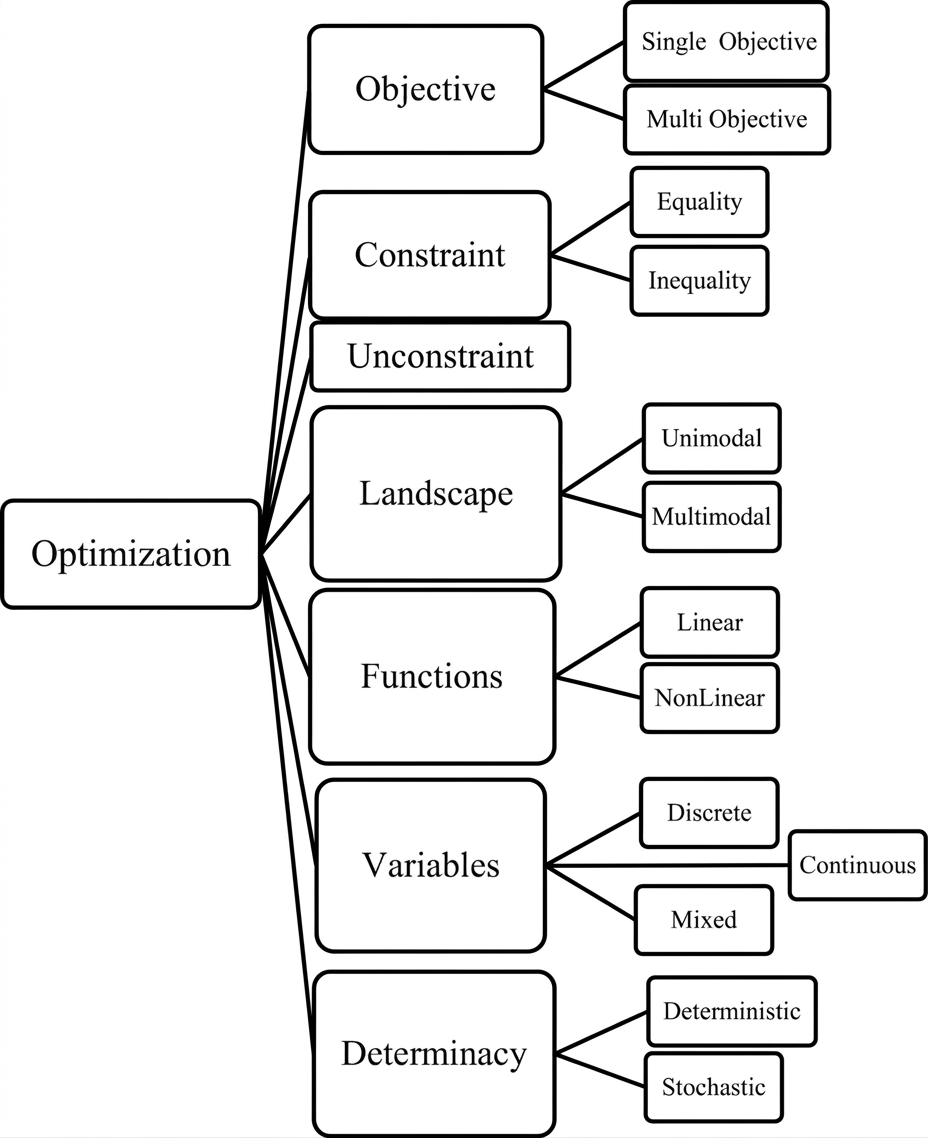
\includegraphics[width=0.48\textwidth]{./figuras/02_fundamentos_teoricos/problems_clasification.png}
    \caption{Taxonomía general de los problemas de optimización tomada de \cite{ahirwal2021swarm}.}
    \label{fig:problems_classification}
\end{figure}

Dentro de esta clasificación general, el presente trabajo se centra en problemas de \textbf{optimización continua monoobjetivo bajo restricciones de caja} (\textit{box constraints}). En este escenario, cada solución candidata deja de ser un elemento abstracto y se representa formalmente mediante un vector de variables reales \(\mathbf{x} = (x_1, x_2, \ldots, x_D)\), donde \(D\) denota la dimensión del problema y cada variable de decisión \(x_i\) toma valores dentro de un intervalo permitido.

De este modo, el marco matemático del problema de minimización considerado en esta investigación se plantea como:
\begin{equation}
    \min_{\mathbf{x} \in S} f(\mathbf{x}),
    \qquad
    S = \prod_{i=1}^{D} [l_i, u_i] \subset \mathbb{R}^{D}
\end{equation}
\noindent donde \(f:S \rightarrow \mathbb{R}\) es la función objetivo escalar, y \(l_i\) y \(u_i\) representan los límites inferior y superior que confinan el intervalo permitido para cada variable de decisión.

Adicionalmente, el alcance de este trabajo se restringe a entornos operativos de \textbf{caja negra} (\textit{black-box optimization}). Esto implica que los algoritmos de búsqueda carezcan de la capacidad de explotar información analítica y derivativa, debiendo guiar su comportamiento únicamente a través del valor escalar obtenido mediante la evaluación directa de soluciones.

En problemas no convexos o multimodales, la presencia de múltiples óptimos locales, mesetas y regiones irregulares dificulta el uso de métodos puramente locales o basados en gradiente. Por ello, resulta necesario recurrir a estrategias de búsqueda capaces de explorar el espacio de soluciones sin depender de información derivativa. Las principales familias de métodos utilizadas con este propósito se presentan en las secciones siguientes.


% Este escenario técnico adquiere su máxima complejidad cuando la superficie de búsqueda es \textbf{no convexa y multimodal}. En este tipo de paisajes, la aparición de múltiples óptimos locales, mesetas y regiones irregulares invalida los métodos de descenso tradicionales, exigiendo el uso de técnicas  ¡de optimización capaces de explorar eficientemente el espacio. Sin embargo, como se introdujo en el Capítulo~\ref{ref:introduccion}, la viabilidad de estos esquemas de búsqueda se ve muy comprometida en escenarios donde la evaluación de la función objetivo conlleva un alto coste computacional o se dispone de un presupuesto estrictamente restringido de evaluaciones. Es precisamente esta limitación fundamental la que restringe el uso de las principales técnicas de optimización y justifica, en última instancia, el desarrollo de las familias algorítmicas y los modelos de sustitución o \textit{surrogates} que se fundamentan en las siguientes secciones de este marco teórico.


% \subsubsection{Según la naturaleza de las variables}

% %% discreta vs continua

% La naturaleza de las variables de decisión determina en gran medida la estructura del problema de optimización. Cuando estas pueden tomar cualquier valor dentro de un intervalo, el problema es continuo. Cuando solo pueden asumir valores aislados o pertenecientes a conjuntos finitos, como ocurre en problemas de selección, asignación o permutación, el problema es discreto. Dentro de esta última categoría ocupan un lugar especialmente relevante los problemas \textbf{combinatorios}, en los que la solución implica seleccionar, asignar u ordenar elementos de entre un conjunto finito de posibilidades.

% Esta distinción resulta especialmente relevante porque influye tanto en la estructura del espacio de búsqueda como en los métodos que pueden emplearse para explorarlo. Mientras que los problemas continuos suelen admitir una modelización matemática más regular, los problemas discretos presentan con frecuencia una mayor complejidad combinatoria, lo que puede dificultar tanto su formulación como su resolución.

% \subsubsection{Según la linealidad del problema}

% % lineal vs no lineal

% La relación que mantienen las variables de decisión con la función objetivo y las restricciones no siempre presenta la misma complejidad. Cuando ambas pueden expresarse mediante relaciones lineales, el problema presenta una estructura más regular y, en general, más fácil de analizar y resolver. Cuando la función objetivo, alguna de las restricciones o ambas incorporan dependencias no lineales, la complejidad del problema aumenta y su resolución suele exigir estrategias más flexibles.

% \subsubsection{Según la convexidad del problema}

% %% convexos vs no convexos

% Una función es convexa si, para cualquier par de puntos en su dominio, el valor que toma sobre cualquier punto del segmento que los une es menor o igual que la combinación convexa de los valores de la función en dichos puntos \cite{boyd2004convex}. En el ámbito de la optimización, esta propiedad resulta especialmente relevante, ya que implica que todo óptimo local es también un óptimo global, lo que facilita la búsqueda de soluciones óptimas.

% Cuando esta condición no se cumple, el problema se considera no convexo. En estos casos, habituales en aplicaciones reales, la superficie de la función objetivo puede presentar múltiples óptimos locales, puntos de silla o regiones irregulares que dificultan el proceso de búsqueda y exige el uso de algoritmos con mayor capacidad de exploración, como las metaheurísticas.


% \subsubsection{Según el número de objetivos}

% En algunos problemas de optimización, la calidad de una solución viene determinada por una única función objetivo, lo que permite comparar directamente las alternativas mediante un solo valor. En otros casos intervienen múltiples objetivos \cite{hakanen2021multiobjective}, cuya optimización conjunta suele resultar más compleja, especialmente cuando entran en conflicto.

% En este contexto, la comparación entre soluciones deja de basarse en un orden total y se apoya habitualmente en el concepto de dominancia de Pareto. Una solución domina a otra si no es peor en ninguno de los objetivos y es mejor en al menos uno de ellos. Por ello, en optimización multiobjetivo no se busca normalmente una única solución óptima, sino un conjunto de soluciones no dominadas, denominado conjunto de Pareto, cuya imagen en el espacio de objetivos recibe el nombre de frente de Pareto \cite{deb2001multiobjective}.

% \subsubsection{Según las restricciones}

% %% con restricciones vs sin restricciones

% La presencia de restricciones \(\Omega\) delimita el conjunto de soluciones factibles y condiciona de forma directa la naturaleza del problema de optimización. En los problemas con restricciones, el objetivo consiste en optimizar la función \(f\) dentro del subconjunto de soluciones que satisfacen dichas condiciones, lo que suele requerir mecanismos específicos para garantizar la factibilidad y, en consecuencia, aumenta la dificultad de resolución. En los problemas sin restricciones, por el contrario, la búsqueda no está limitada por condiciones adicionales y se desarrolla sobre todo el espacio de búsqueda considerado.

\section{Estrategias de resolución: Metaheurísticas}

%% algoritmo aproximado frente a las exactas


%% Dinámicas de búsqueda: Exploración frente a explotación


%% Fenómenos críticos en computación evolutiva: Diversidad, estancamiento y convergencia prematura.

%% (Aquí se inserta el gráfico de Scopus para demostrar el auge del campo).


Debido a la relevancia práctica y teórica de los problemas de optimización en la ingeniería y las ciencias aplicadas, a lo largo del tiempo se ha desarrollado una amplia variedad de metodologías de resolución. Como se esquematiza en la Figura~\ref{fig:clasificacion_tecnicas_optimizacion}, estos enfoques abarcan desde procedimientos exactos, orientados a garantizar matemáticamente el hallazgo del óptimo global sacrificando la viabilidad temporal ante problemas complejos, hasta técnicas aproximadas.

Al trabajar sobre paisajes multimodales, no convexos y bajo condiciones de caja negra (\textit{black-box optimization}), el uso de métodos exactos resulta completamente inviable. Por ello, este trabajo se apoya en el marco operativo de las \textbf{metaheurísticas}, definidas como estrategias de aproximación de propósito general, a menudo no deterministas, que guían de forma eficiente a operadores de búsqueda abstractos con el fin de hallar soluciones de alta calidad en tiempos de cómputo razonables, renunciando a la garantía matemática de optimalidad global \cite{glover1986future, talbi2009metaheuristics, boussaid2013survey, marti2025fifty}.

\begin{figure}[H]
    \centering
    \begin{tikzpicture}[
            scale=0.88,
            transform shape,
            level distance=1.9cm,
            sibling distance=4.3cm,
            every node/.style={
                    rectangle,
                    rounded corners,
                    draw=black,
                    align=center,
                    minimum width=3.0cm,
                    minimum height=0.7cm,
                    font=\small
                },
            root/.style={
                    fill=blue!20,
                    font=\small\bfseries
                },
            levelone/.style={
                    fill=green!20,
                    font=\small\bfseries
                },
            leveltwo/.style={
                    fill=orange!25,
                    font=\small\bfseries
                },
            edge from parent/.style={
                    draw=black,
                    thick
                }
        ]

        \node[root] {Técnicas de\\optimización}
        child { node[levelone] {Técnicas\\exactas} }
        child { node[levelone] {Técnicas\\aproximadas}
                child { node[leveltwo] {Heurísticas} }
                child { node[leveltwo] {Metaheurísticas} }
            };

    \end{tikzpicture}
    \caption{Clasificación general de las técnicas para la resolución de problemas de optimización.}
    \label{fig:clasificacion_tecnicas_optimizacion}
\end{figure}

A diferencia de otras técnicas de aproximación, las metaheurísticas proporcionan un marco más general de búsqueda que puede adaptarse a distintas formulaciones mediante la incorporación de operadores, reglas o mecanismos dependientes del contexto \cite{talbi2009metaheuristics,gendreau2010handbook}. Su propósito no es recorrer exhaustivamente todas las soluciones posibles, sino explorar el espacio de búsqueda de manera eficiente, favoreciendo aquellas regiones que parecen prometedoras y reduciendo el esfuerzo invertido en zonas poco rentables.

Para justificar el impacto y el interés científico de estas metodologías, la Figura~\ref{fig:numero_papers_mh} ilustra la evolución bibliométrica del número de publicaciones indexadas en la base de datos Scopus bajo el término \textit{"metaheuristic"}. El crecimiento exponencial observado a lo largo de las últimas décadas evidencia la consolidación de este campo como una herramienta imprescindible para abordar problemas del mundo real donde los métodos tradicionales fallan.

\begin{figure}[H]
    \centering
    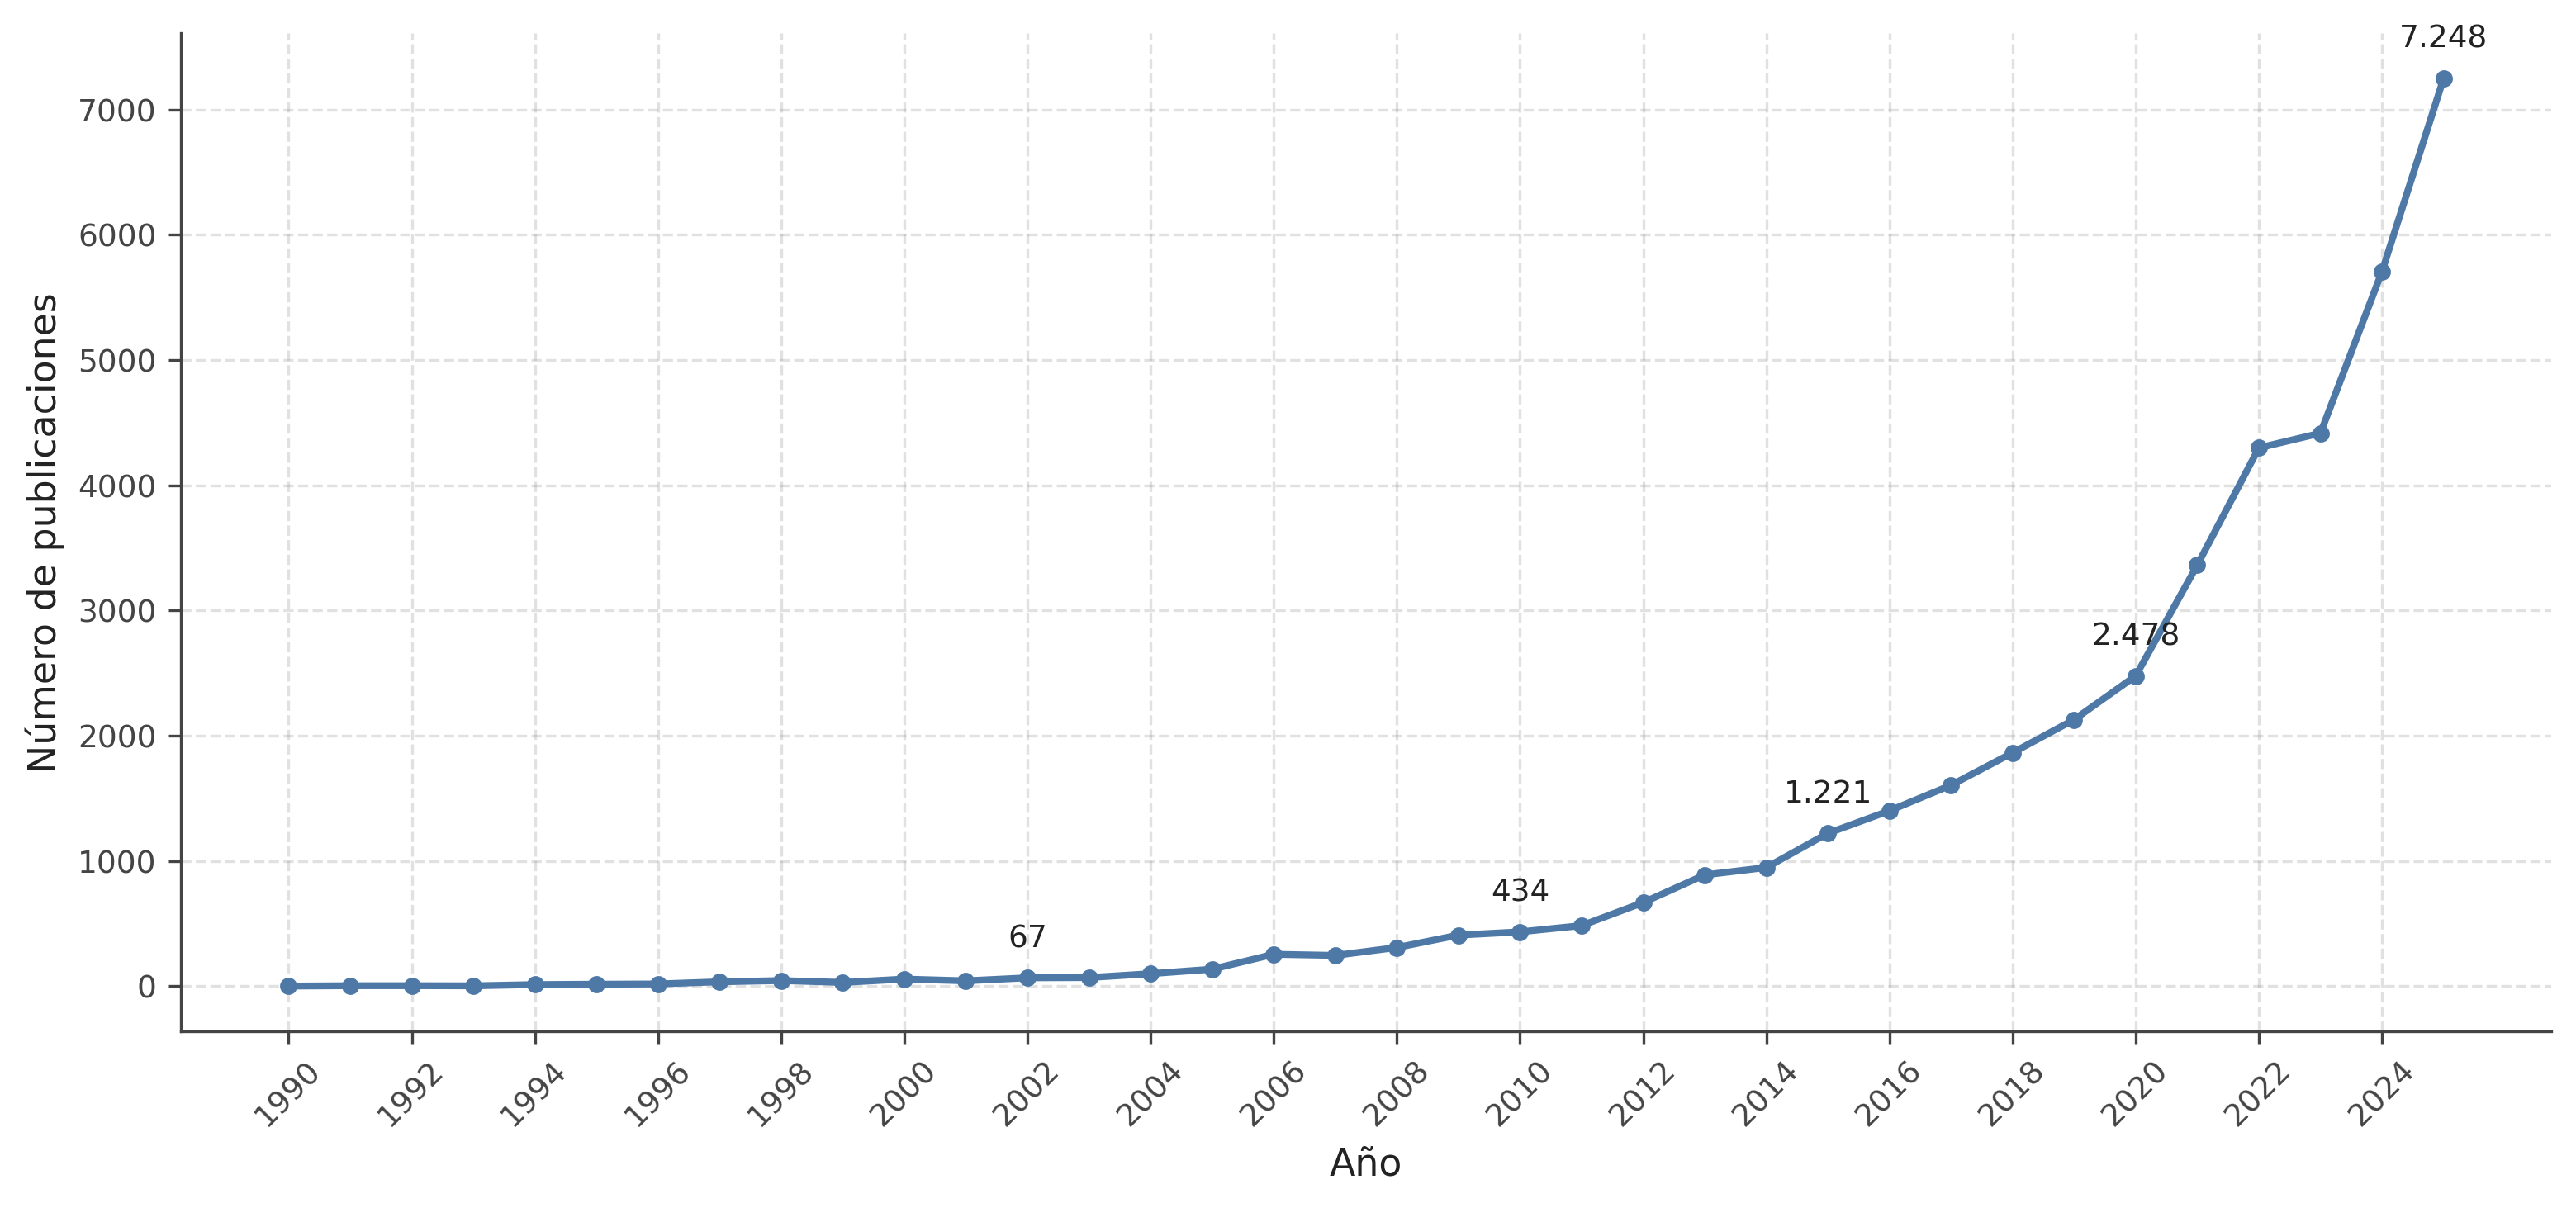
\includegraphics[width=1.0\textwidth]{./figuras/estado_del_arte/metaheuristicas_num_papers.png}
    \caption{Evolución anual del número de publicaciones sobre metaheurísticas en Scopus (1990--2025).}
    \label{fig:numero_papers_mh}
\end{figure}

Desde un punto de vista más abstracto, una metaheurística puede interpretarse como un esquema iterativo general parametrizable. Adaptando la formalización de \cite{luque2006resolucion}, denotamos el método como una tupla:

\begin{equation}
    \mathcal{M}=\langle \Theta,\Phi,\sigma,\mu,\lambda,\Xi,\tau\rangle
\end{equation}
\noindent donde $\Theta$ representa el conjunto de estructuras de trabajo, $\Phi$ el operador que genera nuevas candidatas, $\sigma$ la función que selecciona las estructuras que continúan en la siguiente iteración, $\mu$ y $\lambda$ el número de estructuras mantenidas y generadas, $\Xi$ el conjunto de variables de estado y $\tau$ el criterio de parada.

A partir de estas características generales, las metaheurísticas pueden organizarse según distintos criterios, entre ellos el tipo de estructura sobre la que articulan la búsqueda. Si bien se dividen taxonómicamente entre aquellas \textbf{basadas en trayectoria} ($\mu = 1$, orientadas a la explotación local mediante vecindarios) y las \textbf{basadas en poblaciones} ($\mu > 1$), este proyecto se enfoca exclusivamente en estas últimas.

\subsection{Dinámicas de búsqueda: Exploración, explotación y estancamiento}
\label{subsec:dinamicas_criticas}

Independientemente de la taxonomía o del diseño algorítmico de la metaheurística utilizada, el éxito en la resolución de problemas continuos complejos depende críticamente del balance dinámico entre dos conceptos totalmente opuestos presentes en sus operadores matemáticos:

\begin{definicion}
    La \textbf{exploración} amplía la búsqueda hacia regiones no visitadas del espacio de soluciones $S$ ayudando a evitar óptimos locales, mientras que la \textbf{explotación} intensifica la búsqueda alrededor de las mejores soluciones encontradas hasta el momento para su refinación.
\end{definicion}

\begin{figure}[H]
    \centering
    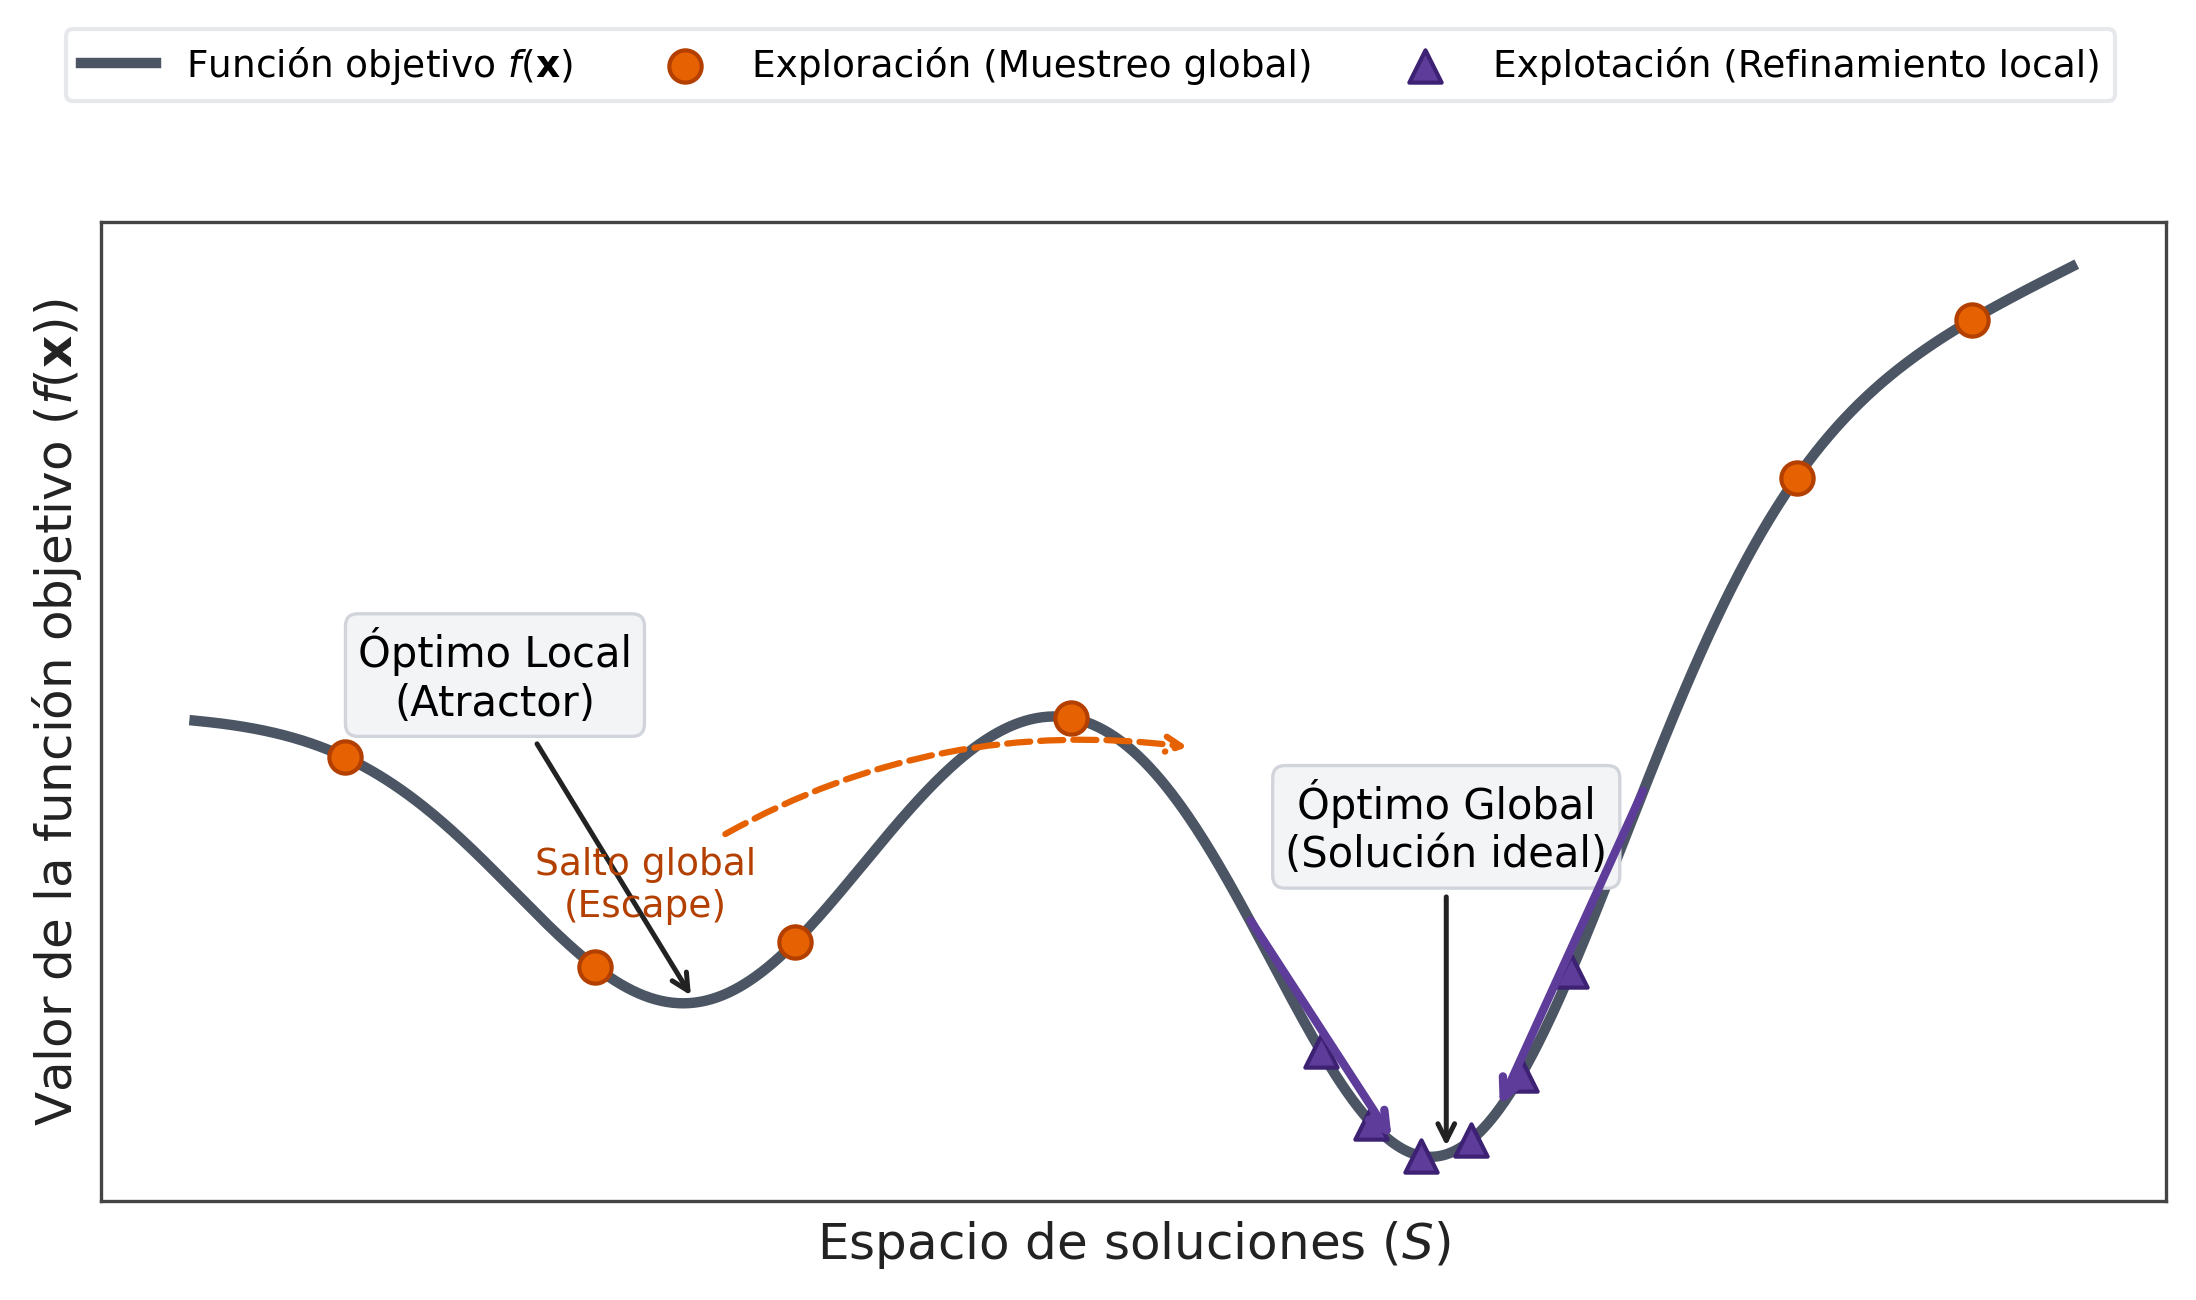
\includegraphics[width=0.8\textwidth]{figuras/02_fundamentos_teoricos/exploracion_explotacion_conceptual.png}
    \caption[Ilustración conceptual de la exploración y la explotación en un paisaje multimodal.]{Ilustración conceptual de la exploración y la explotación en un paisaje multimodal. La exploración distribuye muestras en distintas regiones del espacio de búsqueda, mientras que la explotación concentra la búsqueda alrededor de una zona prometedora para refinar la solución.}
    \label{fig:exploracion_explotacion}
\end{figure}

Durante el proceso iterativo de optimización, debe existir un equilibrio entre ambas fases. No obstante, también puede conducir a una intensificación excesiva o prematura bajo la cual la metaheurística sufre el fenómeno de la \textbf{convergencia prematura} \cite{pandey2014premature}. Este comportamiento ocurre cuando el algoritmo queda atrapado en un óptimo local, perdiendo la capacidad de escapar hacia otras zonas más prometedoras.

Como consecuencia directa de la convergencia prematura o de la caída en mesetas de gradiente nulo, se manifiesta el \textbf{estancamiento} \cite{squillero2016divergence}. Puede decirse que un algoritmo entra en dicha fase cuando, aun continuando con su ejecución, deja de producir mejoras significativas en la calidad de las soluciones durante un número prolongado de iteraciones o evaluaciones. Este comportamiento suele aparecer cuando los operadores quedan confinados en una región cuya explotación adicional apenas genera progreso. Si esta concentración ocurre demasiado pronto, la explotación pasa a dominar de forma excesiva sobre la exploración y el radio de búsqueda útil se colapsa antes de que el método haya revisado de forma suficientemente amplia otras zonas potencialmente prometedoras. En consecuencia, la convergencia prematura puede interpretarse como uno de los principales mecanismos que conducen al estancamiento en los procesos de optimización aproximada.

La mitigación del estancamiento motiva el diseño de estructuras más complejas, como las metaheurísticas poblacionales, así como la introducción de mecanismos de rescate dinámicos.

\subsection{Metaheurísticas basadas en poblaciones}
\label{subsec:mh_poblacion}

Las metaheurísticas basadas en poblaciones se caracterizan por trabajar simultáneamente con un conjunto de soluciones candidatas, a diferencia de los enfoques basados en trayectoria \cite{blum2003metaheuristics,boussaid2013survey}. Esta propiedad les permite mantener activas distintas regiones del espacio de búsqueda $S$ al mismo tiempo y aprovechar la información contenida en la distribución relativa de los individuos para orientar la dinámica del proceso de optimización \cite{talbi2009metaheuristics}.

En términos generales, su funcionamiento parte de una población inicial de soluciones por el espacio continuo $S$ que es evaluada, alterada mediante operadores estocásticos y actualizada aplicando cirerios de selección o reemplazo.

La principal ventaja de esta familia es su elevada capacidad exploratoria al muestrear distintas zonas del espacio de búsqueda e identificar regiones prometedoras, lo que reduce el riesgo de convergencia prematura. Sin embargo, esta ventaja conlleva un mayor coste computacional por ciclo, ya que en cada generación deben evaluarse multiples candidatos.

La propiedad fundamental que permite representar la dinámica de estas soluciones concurrentes y que determina la transición entre la exploración global y la explotación local es la \textbf{diversidad poblacional}:

\begin{definicion}
    La \textbf{diversidad poblacional} hace referencia a la variedad y heterogeneidad de las soluciones candidatas presentes en la población de una metaheurística. Mantener una diversidad adecuada es crucial para evitar el estancamiento y favorecer la exploración efectiva del espacio de búsqueda.
\end{definicion}

A medida que el algoritmo selecciona las regiones de mayor rendimiento, los individuos tienden a agruparse, contrayendo de forma natural la diversidad. No obstante, si esta pérdida de variabilidad ocurre de manera descontrolada, la población colapsa hacia la homogeneidad absoluta, volviendo a los individuos indistinguibles en el espacio continuo y dando lugar al estancamiento.

En el marco de este trabajo, este fenómeno es crítico. Al colapsar la diversidad, la heterogeneidad de las muestras recolectadas disminuye notablemente, provocando que los modelos de regresión y aprendizaje automático pierdan la capacidad estadística para entrenarse eficazmente y discriminar la calidad de nuevos candidatos \cite{omidvar2022review}.

Para mitigar este tipo de situaciones y evitar que el colapso de la diversidad limite tanto la búsqueda como la asistencia del modelo subrogado, pueden incorporarse \textbf{mecanismos de reinicio} encargados de reactivar la exploración cuando se detecta una ausencia prolongada de mejora \cite{fukunaga1998restart,lozano2008replacement}. El mecanismo concreto adoptado en este trabajo se describe en el Capítulo~\ref{chap:algo_tecnicas_ref}.

\subsection{Metaheurísticas evolutivas y operadores de la Computación Evolutiva}
\label{subsec:mh_evolutivas}

Dentro del paradigma de los métodos basados en poblaciones, las  \textbf{metaheurísticas evolutivas} constituyen una de las familias más robustas y ampliamente utilizadas en la literatura para la optimizacion continua  \cite{boussaid2013survey}.

Inspiradas en los mecanismos de adaptación y evolución observados en la naturaleza, estas técnicas hacen evolucionar un conjunto de soluciones candidatas llamado población a lo largo de ciclos iterativos denominados generaciones. Cada individuo se formaliza como un vector de variables reales $\mathbf{x} = (x_1, \dots, x_D) \in \mathbb{R}^D$, cuya adaptación cuantitativa al medio se califica a través de una función de aptitud o \textit{fitness} ($f(\mathbf{x})$) que mide la la calidad de la solución y guía el proceso de búsqueda \cite{talbi2009metaheuristics}.

La dinámica de búsqueda de una metaheurística evolutiva general, desde su inicialización hasta el cumplimiento de los criterios de parada, está determinado por la aplicación de cuatro operadores universales \cite{luke2013essentials}:

\begin{enumerate}
    \item \textbf{Selección de progenitores (o de padres):} Mecanismo encargado de elegir qué individuos de la población actual tendrán prioridad para reproducirse, asegurando que las soluciones con mejor rendimiento (\textit{fitness} más óptimo) transmitan su información a las siguientes iteraciones.
    \item \textbf{Operadores de variación (Cruce y Mutación):} Constituyen el motor de generación de diversidad y exploración del algoritmo:
          \begin{itemize}
              \item \textit{Cruce:} Operador que toma dos o más soluciones seleccionadas como padres e intercambia o combina sus componentes vectoriales para dar lugar a nuevos individuos descendientes (\textit{offspring}). Su papel es explotar y comunicar regiones prometedoras ya descubiertas.
              \item \textit{Mutación:} Operador unario que altera aleatoriamente uno o varios componentes de un vector descendiente. Su papel es puramente exploratorio, introduciendo diversidad para evitar el estancamiento en óptimos locales.
          \end{itemize}
    \item \textbf{Evaluación de soluciones:} Fase en la que se calcula el valor de $f(\mathbf{x})$ para cada nuevo descendiente generado. Si el cálculo de $f(\mathbf{x})$ exige una coste computacional elevado, el coste de evaluar poblaciones enteras de forma recurrente vuelve inviable la optimización evolutiva.
    \item \textbf{Reemplazo (Selección de supervivientes):} Mecanismo encargado de decidir qué elementos, entre la población original y el conjunto de nuevos descendientes, conformarán la población que sobrevive y pasa a la siguiente generación.
\end{enumerate}

De esta manera, la dinámica de un algoritmo evolutivo puede resumirse en el Algoritmo~\ref{alg:ea_general}.

\begin{algorithm}[H]
    \caption{Esquema general de un algoritmo evolutivo}
    \label{alg:ea_general}
    \begin{algorithmic}[1]
        \State $P \gets \textsc{GenerarPoblacionInicial}()$
        \State $\textsc{Evaluar}(P)$
        \While{no se cumpla el criterio de parada}
        \State $P' \gets \textsc{SeleccionarPadres}(P)$
        \State $P' \gets \textsc{Cruzar}(P')$
        \State $P' \gets \textsc{Mutar}(P')$
        \State $\textsc{Evaluar}(P')$
        \State $P \gets \textsc{SeleccionarNuevaPoblacion}(P, P')$
        \EndWhile
        \State \Return mejor solución encontrada
    \end{algorithmic}
\end{algorithm}

Dentro de esta familia se incluyen distintas líneas metodológicas, entre ellas los algoritmos genéticos o las estrategias evolutivas, que comparten el enfoque poblacional y evolutivo, aunque difieren en la forma en que generan nueva descendencia y en los operadores que emplean.


% %% tecnicas de optimizacion

% \begin{figure}[htbp]
%     \centering
%     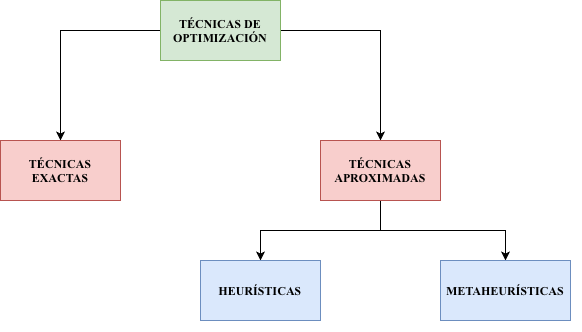
\includegraphics[width=0.85\textwidth]{./figuras/clasificacion_tecnicas_optimizacion/clasificacion_tecnicas_optimizacion.drawio.png}
%     \caption{Clasificación general de las técnicas de optimización.}
%     \label{fig:optimization_methods}
% \end{figure}
%% tecnicas exactas: garantia del optimo

% \subsection{Técnicas exactas}

% Las técnicas exactas constituyen aquellos métodos de optimización que, bajo una formulación adecuada del problema y con un presupuesto de cómputo suficiente, garantizan la obtención de la solución óptima. En este grupo se incluyen, por ejemplo, la programación lineal, la programación entera, la programación dinámica y otros procedimientos matemáticos basados en propiedades estructurales del problema.

% Su principal ventaja reside en que proporcionan garantías teóricas sobre la optimalidad de la solución obtenida. Sin embargo, esta característica suele ir acompañada de una fuerte dependencia de la formulación del problema y de un crecimiento significativo del coste computacional a medida que aumenta la complejidad del espacio de búsqueda. Por ello, cuando el problema es grande, no convexo o carece de una estructura explotable de forma directa, estas técnicas pueden resultar poco adecuadas o incluso inviables en escenarios reales.


% %% tecnicas aproximadas: sacrificio de la garantia del optimo por tiempo

% \subsection{Técnicas aproximadas}

% Aunque las técnicas exactas componen el marco de referencia desde el punto de vista teórico, en la práctica numerosos problemas de optimización deben abordarse mediante métodos aproximados capaces de proporcionar soluciones de calidad aceptable dentro de un presupuesto computacional razonable. Estas técnicas no aseguran, en general, la obtención del óptimo global, pero permiten afrontar problemas de gran escala o elevada complejidad en los que los procedimientos exactos resultan inviables por su coste o por la ausencia de una estructura suficientemente explotable \cite{boussaid2013survey}.

% El interés por este tipo de enfoques se debe a su capacidad para equilibrar calidad de solución y eficiencia temporal. Dentro de esta categoría se distinguen, de forma general, las \textbf{heurísticas} y las \textbf{metaheurísticas}, que constituyen dos de los marcos más utilizados en la optimización moderna. Aunque ambas persiguen soluciones de buena calidad en tiempos razonables, difieren en su alcance, grado de generalidad y capacidad para adaptarse a distintos problemas de optimización.

% %% heuristicas

% \subsubsection{Heurísticas}

% Generalmente, el término \textit{heurística} se utiliza para designar estrategias prácticas de resolución de problemas que permiten orientar la búsqueda de soluciones cuando no resulta viable, o no es necesario, aplicar un procedimiento exacto o exhaustivo \cite{handbookheuristics2018}. En optimización, esta idea se traduce en métodos capaces de explotar de forma eficiente la estructura del problema para obtener soluciones de calidad aceptable.

% \begin{definicion}
%     Las heurísticas son procedimientos de búsqueda orientados a obtener soluciones de buena calidad en un tiempo de cómputo reducido, sin garantizar la optimalidad de la solución obtenida.
% \end{definicion}

% Su interés radica en que permiten abordar problemas complejos en los que la resolución exacta resulta poco práctica debido al elevado coste computacional o al tamaño del espacio de búsqueda \cite{springer2024heuristics}.

% Según la forma en que generan o refinan las soluciones, las heurísticas suelen agruparse en distintas familias \cite{franca1999adaptive}. \textbf{Las heurísticas constructivas} construyen una solución desde cero, incorporando decisiones de manera progresiva hasta completar una solución factible. \textbf{Las heurísticas de mejora} parten de una solución inicial y la refinan mediante modificaciones locales orientadas a incrementar su calidad. \textbf{Las heurísticas híbridas} combinan ambos enfoques o integran estrategias adicionales de búsqueda con el objetivo de aprovechar las ventajas de cada una de ellas \cite{moreira2013hybrid}.

% %% metaheuristicas

% % - son métodos no exactos y, por lo general, no deterministas
% % - guían el proceso de búsqueda
% % - realizan una exploración eficiente del espacio de búsqueda
% % - tienen una estructura básica predefinida
% % - pueden incorporar heurísticos específicos dependientes del problema
% % - usan mecanismos para evitar regiones poco prometedoras
% % - son iterativos y disponen de criterios de parada
% % - persiguen soluciones cuasi óptimas

% % - idea: la armonización entre exploración y explotación como uno de los rasgos clave de la eficiencia de una metaheurística

% \subsubsection{Metaheurísticas}

% Las metaheurísticas constituyen una familia de métodos de optimización no exactos, diseñados para obtener soluciones de alta calidad en tiempos de cómputo razonables, especialmente en problemas complejos para los que los métodos exactos resultan inviables desde un punto de vista práctico \cite{glover1986future,talbi2009metaheuristics,boussaid2013survey}. En términos generales, se trata de procedimientos, a menudo no deterministas, concebidos para guiar de forma eficiente el proceso de búsqueda a través del espacio de soluciones \cite{talbi2009metaheuristics,luke2013essentials,marti2025fifty}.

% A diferencia de las heurísticas específicas de problema, las metaheurísticas proporcionan un marco más general de búsqueda que puede adaptarse a distintas formulaciones mediante la incorporación de operadores, reglas o mecanismos dependientes del contexto \cite{talbi2009metaheuristics,gendreau2010handbook}. Su propósito no es recorrer exhaustivamente todas las soluciones posibles, sino explorar el espacio de búsqueda de manera eficiente, favoreciendo aquellas regiones que parecen prometedoras y reduciendo el esfuerzo invertido en zonas poco rentables.

% En la mayoría de los casos, su funcionamiento se apoya en una estructura básica predefinida sobre la que se construyen mecanismos de generación, evaluación y actualización de soluciones. Este proceso se repite hasta que se satisface algún criterio de parada, como un número máximo de iteraciones, un límite temporal o una condición de convergencia \cite{luke2013essentials}. Como resultado, las metaheurísticas persiguen soluciones de calidad suficientemente alta para numerosos problemas reales, aunque sin garantizar optimalidad global \cite{glover1986future,talbi2009metaheuristics,boussaid2013survey}.

% Uno de los principios fundamentales en el diseño de metaheurísticas es el equilibrio entre exploración y explotación \cite{talbi2009metaheuristics,luke2013essentials,boussaid2013survey}. La exploración permite recorrer distintas regiones del espacio de búsqueda y reducir el riesgo de convergencia prematura, mientras que la explotación concentra el esfuerzo computacional en refinar aquellas zonas que ya han mostrado soluciones prometedoras. La capacidad para armonizar ambos comportamientos constituye uno de los elementos que más influye en la eficacia y robustez de estos métodos.

% Desde un punto de vista más abstracto, una metaheurística puede interpretarse como un esquema iterativo general compuesto por un conjunto de soluciones o estructuras de trabajo, un operador de generación de nuevas candidatas, un mecanismo de selección o reemplazo, un conjunto de variables de estado y un criterio de parada. Esta formalización, adaptada de \cite{luque2006resolucion}, permite describir bajo un mismo marco metaheurísticas de naturaleza muy distinta:
% \[
%     \mathcal{M}=\langle \Theta,\Phi,\sigma,\mu,\lambda,\Xi,\tau\rangle,
% \]
% donde \(\Theta\) es el conjunto de estructuras con las que trabaja el método, \(\Phi\) el operador que genera nuevas candidatas, \(\sigma\) la función que selecciona las estructuras que continúan en la siguiente iteración, \(\mu\) y \(\lambda\) el número de estructuras mantenidas y generadas, \(\Xi\) el conjunto de variables de estado del algoritmo y \(\tau\) el criterio de parada.

% A partir de estas características generales, las metaheurísticas pueden organizarse según distintos criterios, entre ellos el tipo de estructura sobre la que articulan la búsqueda. Esta distinción permite introducir las principales familias de métodos que se describen a continuación.

% \begin{figure}[H]
%     \centering
%     \begin{tikzpicture}[
%         node distance=0.8cm and 2.3cm,
%         every node/.style={font=\scriptsize},
%         box/.style={
%                 draw,
%                 rounded corners,
%                 align=center,
%                 minimum height=0.6cm,
%                 minimum width=2.4cm
%             },
%         rootbox/.style={
%                 box,
%                 fill=gray!15,
%                 text width=2.6cm
%             },
%         childbox/.style={
%                 box,
%                 fill=blue!8,
%                 text width=2.3cm
%             },
%         subclass/.style={
%                 box,
%                 fill=gray!3,
%                 text width=2.1cm
%             },
%         arrow/.style={
%         -{Latex[length=2mm]},
%         thick
%         }
%         ]

%         \node[rootbox] (root) {Metaheurísticas};
%         \node[childbox, below left=1.1cm and 1.5cm of root] (pop) {Basadas en\\población};
%         \node[childbox, below right=1.1cm and 0.8cm of root] (tray) {Basadas en\\trayectoria};

%         \matrix (subpops) [below=2.0cm of pop, column sep=1.8cm, row sep=0cm] {
%             \node[subclass] (enjambre) {Basadas en\\inteligencia de enjambre}; &
%             \node[subclass] (hibridas) {Híbridas};                             &
%             \node[subclass] (evolutivas) {Evolutivas};                           \\
%         };

%         \draw[arrow] (root) -- (pop);
%         \draw[arrow] (root) -- (tray);

%         \draw[arrow] (pop) -- (enjambre);
%         \draw[arrow] (pop) -- (hibridas);
%         \draw[arrow] (pop) -- (evolutivas);

%     \end{tikzpicture}
%     \caption{Clasificación general de las metaheurísticas según el tipo de estructura de búsqueda.}
%     \label{fig:clasificacion_metaheuristicas}
% \end{figure}

% \paragraph{Metaheurísticas basadas en trayectoria}

% Las metaheurísticas basadas en trayectoria se caracterizan por trabajar, en cada iteración, sobre una única solución actual o sobre un número muy reducido de soluciones estrechamente relacionadas \cite{blum2003metaheuristics,boussaid2013survey}. A partir de esa solución, el algoritmo genera nuevas candidatas mediante movimientos definidos sobre su vecindario, de modo que la búsqueda va construyendo una trayectoria a través del espacio de soluciones \cite{talbi2009metaheuristics}.

% En muchos casos, estos métodos se consideran extensiones de los procedimientos clásicos de búsqueda local. Mientras que una búsqueda local simple suele detenerse al alcanzar un óptimo local, las metaheurísticas basadas en trayectoria incorporan mecanismos adicionales para escapar de esas regiones y continuar explorando otras zonas del espacio de búsqueda \cite{gendreau2010handbook,luke2013essentials}. Entre dichos mecanismos pueden encontrarse la aceptación controlada de soluciones peores, el uso de memoria o la modificación del vecindario.

% Su principal ventaja reside en que permiten intensificar la búsqueda de manera muy eficiente alrededor de soluciones prometedoras. Sin embargo, esta misma concentración sobre una única trayectoria puede reducir la diversidad explorada y aumentar el riesgo de convergencia prematura si no se incorporan mecanismos adecuados de diversificación \cite{blum2003metaheuristics,boussaid2013survey}. Dentro de esta familia se incluyen metaheurísticas como \textit{Simulated Annealing} \cite{kirkpatrick1983optimization,vanderbilt1984monte,pedamallu2008investigating}, \textit{Tabu Search} \cite{glover1989tabu,rachid2000tabu} o \textit{Variable Neighborhood Search}. Desde la formalización abstracta introducida anteriormente, este comportamiento se corresponde típicamente con el uso de una única estructura activa por iteración, de modo que \(\mu = 1\), y con la generación de un número reducido de nuevas estructuras, por lo que \(\lambda\) suele ser pequeño.

% \paragraph{Metaheurísticas basadas en poblaciones}

% Las metaheurísticas basadas en poblaciones se caracterizan por trabajar simultáneamente con un conjunto de soluciones candidatas, en lugar de guiar la búsqueda a partir de una única solución actual \cite{blum2003metaheuristics,boussaid2013survey}. Esta característica les permite mantener activas distintas regiones del espacio de búsqueda al mismo tiempo y aprovechar la información contenida en la distribución relativa de los individuos para orientar la evolución del proceso de optimización \cite{talbi2009metaheuristics,luke2013essentials}.

% En términos generales, su funcionamiento parte de una población inicial de soluciones, a partir de la cual se generan nuevas candidatas utilizando la información disponible en los individuos ya presentes. Posteriormente, dichas soluciones se evalúan y la población se actualiza según algún criterio de selección o reemplazo \cite{talbi2009metaheuristics,boussaid2013survey}. El intercambio de información entre soluciones puede modelarse de distintas maneras, como la recombinación entre individuos, el uso de diferencias entre soluciones o la atracción hacia posiciones prometedoras.

% Una de las principales ventajas de esta familia es su elevada capacidad exploratoria. Al mantener múltiples soluciones simultáneamente, las metaheurísticas poblacionales pueden muestrear distintas zonas del espacio de búsqueda, identificar regiones prometedoras y reducir el riesgo de convergencia prematura asociado a la concentración temprana en una sola trayectoria \cite{blum2003metaheuristics,boussaid2013survey,omidvar2022review}. No obstante, esta ventaja suele ir acompañada de un mayor coste computacional por iteración, ya que en cada ciclo deben evaluarse varias soluciones candidatas. Esta observación resulta especialmente relevante en problemas con funciones objetivo costosas, donde el uso de grandes poblaciones puede hacer necesario recurrir a estrategias de aceleración, paralelización o modelado \textit{surrogate} \cite{omidvar2022review}.

% Desde la formalización abstracta introducida anteriormente, las metaheurísticas basadas en poblaciones se caracterizan por operar con varias estructuras activas en cada iteración, por lo que \(\mu > 1\). Del mismo modo, el número de nuevas estructuras generadas en cada ciclo también suele ser superior al de los métodos basados en trayectoria, de manera que \(\lambda > 1\).

% \subparagraph{Metaheurísticas poblacionales basadas en inteligencia de enjambre}

% Las metaheurísticas basadas en inteligencia de enjambre modelan comportamientos colectivos descentralizados, en los que múltiples agentes interactúan entre sí y con el entorno para orientar la búsqueda. En esta familia se sitúan, entre otros, \textit{Particle Swarm Optimization} \cite{kennedy1995pso} o \textit{Ant Colony Optimization} \cite{socha2008aco}.

% \subparagraph{Metaheurísticas poblacionales híbridas}

% Las metaheurísticas híbridas poblacionales combinan mecanismos de búsqueda poblacional con procedimientos adicionales de intensificación, como búsqueda local o estrategias meméticas, con el objetivo de combinar exploración global y refinamiento local \cite{lozano2004memetic,ong2004metalamarckian,renders1996hybrid,hart1994adaptive}. Dentro de este panorama también pueden situarse enfoques basados en modelado probabilístico, como los \textit{Estimation of Distribution Algorithms} \cite{ahn2008eda}.

% \subparagraph{Metaheurísticas poblacionales evolutivas}

% Los algoritmos evolutivos (EA) constituyen una familia de metaheurísticas poblacionales inspiradas en los mecanismos de adaptación y evolución observados en la naturaleza. De forma general, operan sobre una población de individuos que representan soluciones candidatas al problema. A lo largo del proceso de búsqueda, dicha población evoluciona mediante operadores de selección, variación y reemplazo \cite{holland1975adaptation,mitchell1998introduction,reeves2003genetic,affenzeller2009genetic}. Cada individuo recibe una valoración cuantitativa a través de una función de aptitud o \textit{fitness}, que mide la calidad de la solución representada y guía el proceso de búsqueda.

% De forma abstracta, la dinámica de un algoritmo evolutivo puede resumirse en el Algoritmo~\ref{alg:ea_general}. En primer lugar, se genera una población inicial y se evalúa su calidad. A continuación, mientras no se satisfaga el criterio de parada, se seleccionan progenitores, se aplican operadores de recombinación y mutación para generar descendencia, se evalúan los nuevos individuos y se actualiza la población mediante algún mecanismo de reemplazo. El proceso iterativo finaliza devolviendo la mejor solución encontrada.

% \begin{algorithm}[H]
%     \caption{Esquema general de un algoritmo evolutivo}
%     \label{alg:ea_general}
%     \begin{algorithmic}[1]
%         \State $P \gets \textsc{GenerarPoblacionInicial}()$
%         \State $\textsc{Evaluar}(P)$
%         \While{no se cumpla el criterio de parada}
%         \State $P' \gets \textsc{SeleccionarPadres}(P)$
%         \State $P' \gets \textsc{Recombinar}(P')$
%         \State $P' \gets \textsc{Mutar}(P')$
%         \State $\textsc{Evaluar}(P')$
%         \State $P \gets \textsc{SeleccionarNuevaPoblacion}(P, P')$
%         \EndWhile
%         \State \Return mejor solución encontrada
%     \end{algorithmic}
% \end{algorithm}

% Dentro de esta familia se incluyen distintas líneas metodológicas, entre ellas los algoritmos genéticos, las estrategias evolutivas y métodos posteriores como \textit{Differential Evolution}, que comparten el enfoque poblacional y evolutivo, aunque difieren en la forma en que generan nueva descendencia y en los operadores que emplean.


\section{Aprendizaje Automático Orientado a la Regresión}
\label{sec:aprendizaje_automatico}

Si bien el campo de la optimización metaheurística se centra en el diseño de estrategias eficientes para explorar espacios de búsqueda complejos, la computación moderna ofrece otro gran paradigma para abordar problemas de caja negra: el \textbf{Aprendizaje Automático} (\textit{Machine Learning}). Aunque históricamente ambas disciplinas han evolucionado como comunidades científicas independientes y con objetivos diferenciados, su convergencia metodológica proporciona hoy en día un marco robusto para la resolución de problemas de alta complejidad computacional.

A diferencia de los enfoques algorítmicos tradicionales, el Aprendizaje Automático es un subcampo de la inteligencia artificial que no pretende codificar instrucciones explícitas para resolver una tarea, sino que dota a los sistemas informáticos de la capacidad de aprender y extraer patrones de los datos sin necesidad de ser programados explícitamente \cite{mitchell1997machine, bishop2006pattern}.


\subsection{Formalización de los conjuntos de datos en el aprendizaje}

Para comprender cómo un sistema computacional extrae conocimiento, es necesario formalizar matemáticamente los componentes informacionales que se requieren. Desde una perspectiva formal, la información disponible se estructura a partir de un conjunto global de observaciones realizadas a partir del conjunto de datos denotado como:

\begin{equation}
    \mathcal{D} = \{(\mathbf{x}_1, y_1), (\mathbf{x}_2, y_2), \dots, (\mathbf{x}_N, y_N)\} = \{(\mathbf{x}_i, y_i)\}_{i=1}^N
\end{equation}

\noindent donde $\mathbf{x}_i \in \mathbb{R}^D$ representa el vector de características (que en el contexto de este proyecto se corresponderá con las variables de decisión de un candidato) e $y_i$ constituye la etiqueta o respuesta real asociada (la evaluación real del problema).

Con el fin de garantizar un aprendizaje correcto y evitar estimaciones sesgadas u optimistas basadas en la mera memorización de datos (\textbf{sobreajuste}), la metodología del Aprendizaje Automático exige la partición estricta de $\mathcal{D}$ en subconjuntos disjuntos y especializados con propósitos bien definidos \cite{bishop2006pattern}:

\begin{itemize}
    \item \textbf{Conjunto de entrenamiento ($\mathcal{D}_{\text{train}}$):} Subconjunto de datos utilizado para ajustar los parámetros del modelo mediante el algoritmo de aprendizaje.
    \item \textbf{Conjunto de validación ($\mathcal{D}_{\text{val}}$):} Subconjunto independiente que no interviene en el entrenamiento que se emplea para evaluar el rendimiento del modelo durante el proceso de desarrollo y para ajustar sus hiperparámetros. Su objetivo es proporcionar una estimación no sesgada del rendimiento del modelo y ayudar a prevenir el sobreajuste, guiando la selección del modelo y su configuración final.
\end{itemize}

\begin{figure}[htbp]
    \centering
    \begin{tikzpicture}[
            node distance = 0.8cm and 1.5cm,
            block/.style = {rectangle, draw, fill=blue!10, minimum width=3.5cm, minimum height=1.2cm, align=center, rounded corners, font=\small},
            trainblock/.style = {rectangle, draw, fill=green!10, minimum width=4cm, minimum height=1.2cm, align=center, rounded corners, font=\small},
            valblock/.style = {rectangle, draw, fill=orange!10, minimum width=4cm, minimum height=1.2cm, align=center, rounded corners, font=\small}
        ]
        % Nodo principal
        \node [block] (dataset) {Conjunto Global $\mathcal{D}$\\ (Histórico de Evaluaciones)};

        % Nodos de partición (Entrenamiento y Validación)
        \node [trainblock, above right=of dataset] (train) {Conjunto de Entrenamiento $\mathcal{D}_{\text{train}}$\\ ($\approx 70-80\%$)};
        \node [valblock, below right=of dataset] (val) {Conjunto de Validación $\mathcal{D}_{\text{val}}$\\ ($\approx 20-30\%$)};

        % Flechas de flujo
        \draw [->, thick] (dataset.east) -- ++(0.5,0) |- (train.west);
        \draw [->, thick] (dataset.east) -- ++(0.5,0) |- (val.west);

        % Indicador de exclusión mutiva (Conjuntos disjuntos)
        \path (train) -- node[font=\scriptsize\color{red!80!black}, fill=white, inner sep=2pt] (disjoint) {$\mathcal{D}_{\text{train}} \cap \mathcal{D}_{\text{val}} = \emptyset$} (val);
        \draw [dashed, red!50] (train.south) -- (val.north);

    \end{tikzpicture}
    \caption{Esquema metodológico de la partición del conjunto global $\mathcal{D}$ en los subconjuntos disjuntos de entrenamiento ($\mathcal{D}_{\text{train}}$) y validación ($\mathcal{D}_{\text{val}}$).}
    \label{fig:particion_datos}
\end{figure}

\subsection{Paradigmas de aprendizaje y el enfoque supervisado}

Una vez definidos estos bloques fundamentales de información, la naturaleza y la disponibilidad de $\mathcal{D}_{\text{train}}$ y $\mathcal{D}_{\text{val}}$ permiten delimitar formalmente los cuatro grandes paradigmas del Aprendizaje Automático \cite{russell2020artificial}:

\begin{itemize}
    \item \textbf{Aprendizaje supervisado:} El conjunto de entrenamiento con el que se alimenta al algoritmo incluye las soluciones deseadas, denominadas etiquetas. El objetivo del algoritmo es aprender un mapeo generalizable que asocie nuevas entradas con sus salidas correspondientes.
    \item \textbf{Aprendizaje semi-supervisado:} Etiquetar los datos suele llevar mucho tiempo y ser costoso, por lo que el conjunto de entrenamiento tiene a muchos casos sin etiquetar y pocos casos etiquetados.
    \item \textbf{Aprendizaje no supervisado:} El algoritmo recibe un conjunto de datos sin etiquetas ni respuestas asociadas, siendo su objetivo descubrir patrones dentro del espacio de características.
    \item \textbf{Aprendizaje por refuerzo:} A diferencia de los enfoques anteriores, el algoritmo no aprende a partir de un conjunto de datos estático con etiquetas, sino que interactúa con un entorno dinámico y aprende una política de decisión que maximiza una recompensa acumulada.
\end{itemize}

Este trabajo se apoya estrictamente en el marco del \textbf{aprendizaje supervisado}.

%% evaluar si aqui hay que explicar los distainos problemas regrsion clasifiacjon
\subsection{El problema de la regresión continua}

%% esta bien definida la regresion o no

Dentro del aprendizaje supervisado, la naturaleza de la variable de salida \(y\) determina el tipo de problema a resolver. Cuando la respuesta pertenece a un conjunto discreto o categórico, el escenario se define como un problema de \textit{clasificación}. Por el contrario, cuando la variable de salida es numérica y continua, \(y \in \mathbb{R}\), se trata de un problema de \textbf{regresión}.

\begin{figure}[H]
    \centering
    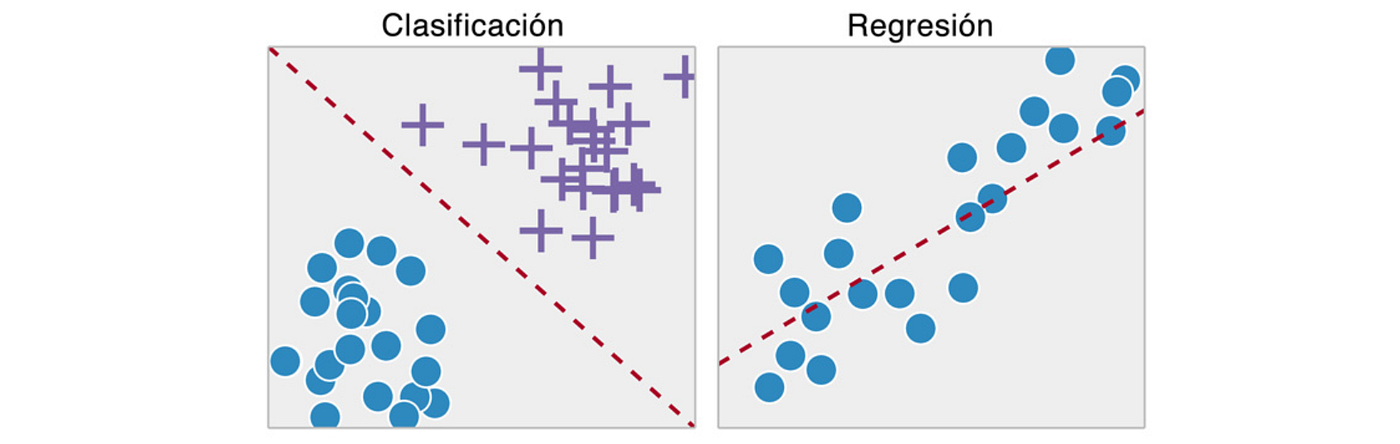
\includegraphics[width=0.7\textwidth]{figuras/02_fundamentos_teoricos/diferencia_clasificacion_regresion.png}
    \caption{Ilustración comparativa entre problemas de clasificación y regresión.}
    \label{fig:regresion_vs_clasificacion}
\end{figure}

Este trabajo se enmarca en el ámbito de la regresión, ya que en optimización continua cada vector de decisión \(\mathbf{x}_i\) tiene asociado un valor real de calidad dado por la función objetivo \(f(\mathbf{x}_i)\). El propósito del modelo supervisado consiste, por tanto, en aprender una aproximación de la relación entre las soluciones candidatas y sus valores de \textit{fitness} a partir de las muestras recolectadas en el conjunto \(\mathcal{D}_{\text{train}}\).

% En este contexto, los modelos de aprendizaje automático actúan como aproximadores predictivos basados en datos. A partir de un conjunto finito de evaluaciones previas, tratan de estimar el valor de la función objetivo en nuevas soluciones candidatas para que la función objetivo real únicamente evalúe las mejores, proporcionando un sustituto computacionalmente más ligero que la evaluación directa del problema original.

\subsection{Taxonomía general de los modelos de regresión}

Para abordar la aproximación predictiva de la función de aptitud a partir de las muestras de $\mathcal{D}_{\text{train}}$, la literatura científica ofrece una amplia diversidad de enfoques algorítmicos en función de cómo modelan la relación entre las variables de entrada (en este contexto, variables de decisión) y el espacio de salida.

A continuación, se describen las cinco grandes filosofías de modelado predictivo para tareas de regresión continua, sentando las bases teóricas de los paradigmas que se compararán en este trabajo.

\subsubsection{Modelos lineales}

Esta familia constituye el pilar histórico de la estadística descriptiva y el aprendizaje supervisado. Su principio operativo asume que la variable de salida se puede aproximar mediante una combinación lineal ponderada de las variables de entrada, donde cada característica es ponderada por un coeficiente numérico que el algoritmo debe optimizar.


% Aunque su capacidad para capturar interacciones no lineales de alta complejidad o paisajes de \textit{fitness} extremadamente rugosos es intrínsecamente limitada (bajo sesgo y alta varianza en escenarios complejos), su velocidad de cómputo es prácticamente instantánea y ofrecen una interpretabilidad absoluta. En el contexto de los modelos subrogados, su uso es altamente valioso como línea base descriptiva (\textit{baseline}) y para aproximar tendencias globales en regiones locales del espacio de búsqueda.

Aunque su capacidad para capturar interacciones no lineales complejas es limitada, su velocidad de cómputo es prácticamente instantánea, no requieren configuraciones complejas y ofrecen una interpretabilidad matemática directa sobre la contribución global de cada variable en el modelo predictivo. Dentro de esta familia se encuentran, por ejemplo, la regresión lineal ordinaria o las variantes regularizadas como Ridge, LASSO o Elastic Net, las cuales introducen penalizaciones matemáticas para controlar la varianza y la complejidad del modelo.

\subsubsection{Modelos basados en árboles y ensambles}

Estos enfoques sustituyen la búsqueda de una función matemática global por una estrategia de particionado recursivo del espacio de características. El modelo base segmenta el dominio de manera jerárquica mediante umbrales lógicos, aislando las muestras en regiones disjuntas denominadas hojas, donde la predicción se establece como el valor promedio de los datos locales de entrenamiento (como se ilustra en la Figura \ref{fig:arbol_decision_regresion}).

\begin{figure}[H]
    \centering
    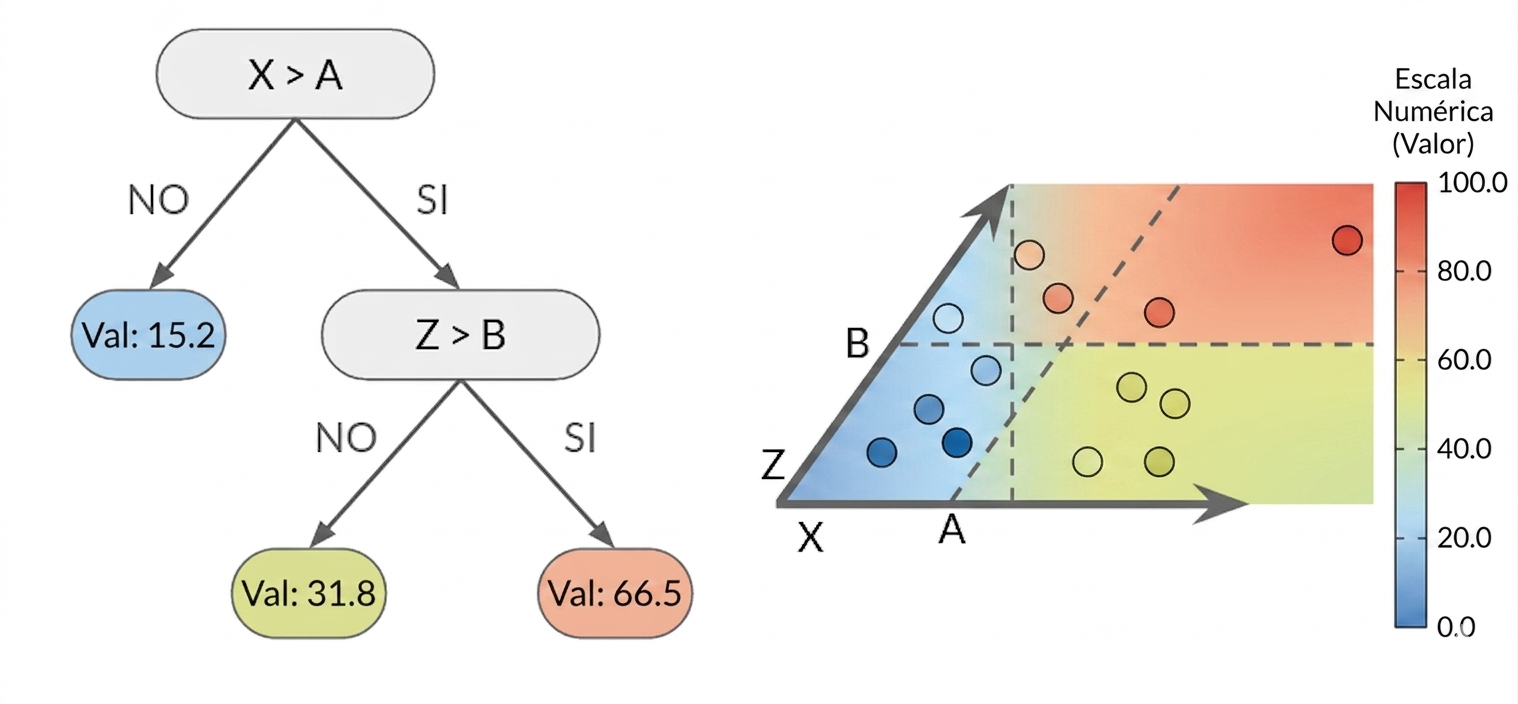
\includegraphics[width=0.7\textwidth]{figuras/02_fundamentos_teoricos/arbol_decision_regresion.png}
    \caption[Ejemplo conceptual de un árbol de decisión aplicado a regresión.]{Ejemplo conceptual de un árbol de decisión aplicado a regresión, donde el espacio de entrada se divide mediante reglas sucesivas hasta asignar una predicción numérica en cada región terminal.}
    \label{fig:arbol_decision_regresion}
\end{figure}

Para suavizar las predicciones escalonadas características de un único árbol de regresión y mitigar su tendencia al sobreajuste, las técnicas modernas recurren a los métodos de ensamble. Estos enfoques combinan las predicciones de múltiples árboles mediante estrategias de agregación en paralelo a través de remuestreo (\textit{bagging}, como en \textit{Random Forest}) o mediante la corrección secuencial y aditiva de los errores residuales de los estimadores previos (\textit{boosting}, como en los algoritmos de \textit{Gradient Boosting} o XGBoost), adaptándose con gran precisión y robustez a las discontinuidades del espacio.

\subsubsection{Modelos basados en vectores de soporte y aprendizaje estadístico}

%% deberiamos citar que es eso del aprendizaje estadistico

Nacidos de la teoría del aprendizaje estadístico, estos modelos abordan la regresión desde una perspectiva geométrica y de optimización convexa.

Su principio básico consiste en buscar una función aproximadora con buena capacidad de generalización, evitando ajustar de forma exacta todas las observaciones del conjunto de entrenamiento. Esta idea se formaliza mediante un margen de tolerancia alrededor de la función predicha. Los errores que quedan dentro de dicho margen no se penalizan, mientras que solo las muestras que lo exceden influyen de forma efectiva en el ajuste del modelo. Estas muestras relevantes reciben el nombre de \textbf{vectores de soporte}, ya que determinan la forma final de la función aprendida.

Una característica relevante de esta familia es el uso de funciones \textit{kernel}, que permiten trabajar de forma implícita en espacios de mayor dimensión sin construir explícitamente dicha transformación, siendo la técnica de Regresión por Vectores de Soporte (\textit{Support Vector Regression}, SVR) el máximo exponente de esta filosofía predictiva en problemas de salida continua.

\subsubsection{Métodos de vecindad y funciones de base}

Esta familia predictiva se basa en la similitud y localidad de los datos: aquellas observaciones que se encuentren a una distancia espacial reducida dentro del dominio de entrada deben presentar valores de salida similares.

Estos métodos computan la predicción de una nueva instancia calculando una interpolación o promedio ponderado de los puntos conocidos más cercanos de $\mathcal{D}_{\text{train}}$, donde la influencia de cada muestra disminuye a medida que aumenta su distancia geométrica respecto al punto a predecir. En esta categoría pueden situarse métodos como \(k\)-Nearest Neighbors para regresión, aproximadores basados en funciones de base radial (RBF) o técnicas de interpolación local.

\subsubsection{Redes neuronales artificiales (\textit{Deep Learning})}

Inspiradas en las dinámicas de transmisión de información de los sistemas biológicos, las redes neuronales estructuran el aprendizaje mediante el encadenamiento jerárquico y masivo de capas de unidades elementales de procesamiento (neuronas artificiales), tal y como se detalla en la Figura \ref{fig:redes_neuronales}, capaces de capturar patrones y relaciones altamente complejas y no lineales.

\begin{figure}[H]
    \centering
    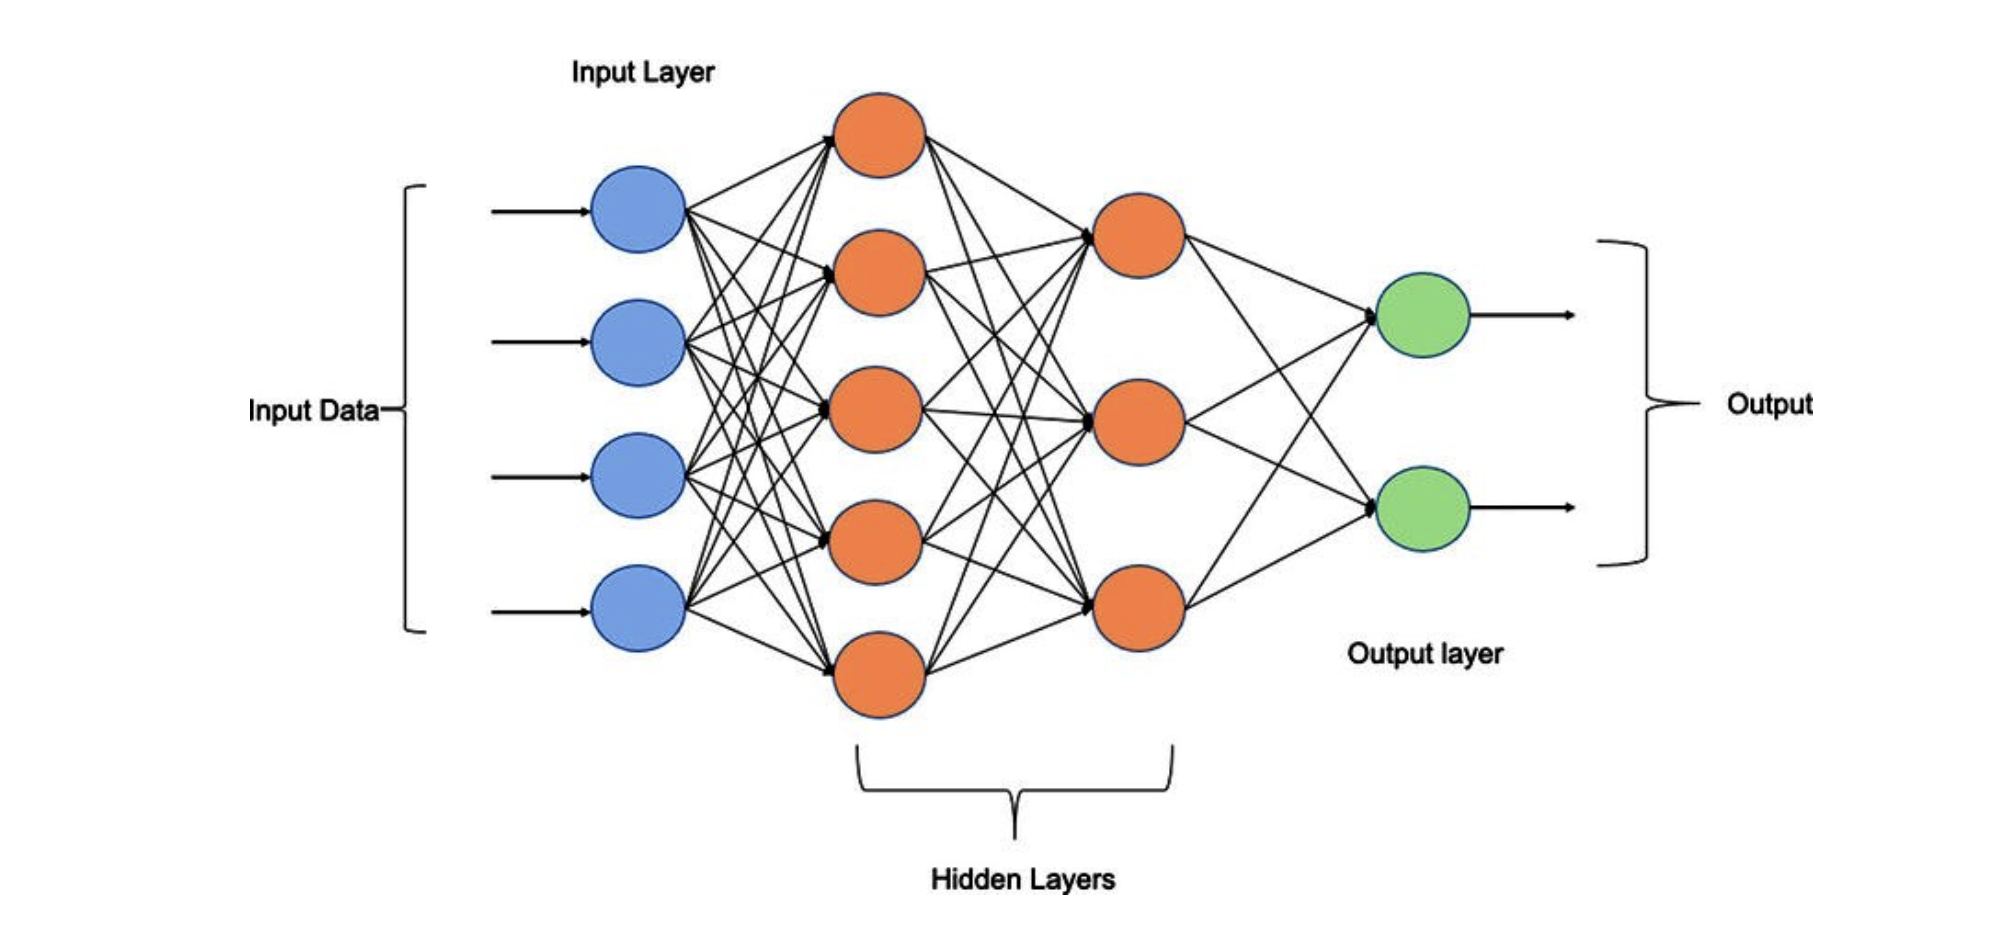
\includegraphics[width=0.65\textwidth]{figuras/02_fundamentos_teoricos/redes_neuronales.png}
    \caption{Esquema conceptual de una red neuronal artificial organizada en capas de entrada, capas ocultas y capa de salida.}
    \label{fig:redes_neuronales}
\end{figure}

Este entrelazado sucesivo de transformaciones les capacita para inducir automáticamente representaciones abstractas de los datos de entrada a lo largo de sus capas, lo que les permite modelar interacciones continuas de extrema complejidad matemática a costa de una mayor demanda de recursos computacionales para su ajuste. El Perceptrón Multicapa (\textit{Multilayer Perceptron}, MLP) asenta las bases clásicas de esta familia en tareas de regresión, asumiendo como contrapartida una alta demanda de recursos computacionales y un volumen de datos elevado para su correcto ajuste.

%% Fundamentos del aprendizaje supervisado y la regresión técnica
%% Taxonomía general de modelos basados en datos: Modelos lineales, basados en árboles (ensamblados) y redes neuronales (Deep Learning) a nivel conceptual.

%% definir los distintos tipos de aprendizaje, destacandno el supervisoda, que es donde se encuentra la regresion.

\section{Técnicas Subrogadas}
\label{sec:tecnicas_subrogadas}

En problemas de optimización continua, una de las principales limitaciones prácticas aparece cuando la evaluación de la función objetivo requiere un coste computacional elevado. Esta situación es habitual en problemas de caja negra basados en simulaciones, modelos físicos, análisis numéricos complejos o procesos experimentales, donde cada evaluación puede implicar un tiempo de cálculo elevado o incluso prohibitivo \cite{queipo2005surrogate,forrester2009recent}. En estos escenarios, una metaheurística poblacional puede necesitar miles de evaluaciones para explorar adecuadamente el espacio de búsqueda, haciendo que el coste total del proceso resulte difícilmente asumible.

Las \textbf{técnicas subrogadas} surgen como una estrategia para reducir este coste. Su idea fundamental consiste en construir un modelo aproximado de la función objetivo a partir de un conjunto limitado de soluciones ya evaluadas. Dicho modelo, denominado modelo subrogado, permite estimar de forma rápida la calidad de nuevas soluciones candidatas sin recurrir siempre a la evaluación real del problema \cite{queipo2005surrogate,forrester2009recent,jin2011surrogate}.

Sea \(f:\mathcal{X}\rightarrow\mathbb{R}\) una función objetivo costosa de evaluar, un modelo subrogado es una aproximación construida a partir de un conjunto finito de muestras evaluadas
\[
    \mathcal{D}=\{(\mathbf{x}_i,f(\mathbf{x}_i))\}_{i=1}^{n},
\]
cuyo propósito es proporcionar información útil sobre el comportamiento de \(f\) con un coste computacional significativamente menor que el de la evaluación directa. Habitualmente, esta información se materializa en una función predictiva \(\hat{f}:\mathcal{X}\rightarrow\mathbb{R}\), aunque también puede adoptar otras formas abstractas orientadas a comparar, clasificar o priorizar soluciones.

Desde esta perspectiva, los modelos subrogados no constituyen una familia independiente de algoritmos de optimización, sino una forma específica de utilizar modelos predictivos dentro del proceso de búsqueda.

Históricamente, esta función ha sido desempeñada tanto por aproximaciones estadísticas y matemáticas clásicas, como \textit{Kriging}, procesos gaussianos o expansiones de caos polinómico (\textit{Polynomial Chaos Expansion}, PCE), como por modelos modernos de aprendizaje automático. Estos últimos pueden actuar como subrogados cuando se entrenan con pares \((\mathbf{x}, f(\mathbf{x}))\) y se emplean, bajo un enfoque de regresión supervisada, para aproximar la relación entre una solución candidata y su valor de \textit{fitness}. Por tanto, la diferencia no reside únicamente en el modelo empleado, sino en el papel que este desempeña: sustituir, apoyar o guiar parcialmente las evaluaciones reales de la función objetivo.

Aunque los modelos subrogados suelen plantearse como aproximaciones directas de la función objetivo, su utilidad en optimización no se limita necesariamente a predecir con total precisión el valor numérico de \(f\). En muchos casos, resulta suficiente con que proporcionen información útil para orientar la búsqueda, por ejemplo preservando el orden relativo entre soluciones, discriminando entre candidatas prometedoras y no prometedoras o apoyando decisiones de selección sin necesidad de reproducir exactamente la función original. Esta distinción permite clasificar las técnicas subrogadas en función del tipo de información que intentan predecir como modelos orientados al \textbf{fitness absoluto} o modelos orientados al \textbf{fitness relativo} \cite{tong2021surrogate}.

\subsection{Clasificación según el tipo de predicción}
\label{subsec:clasificacion_surrogates_prediccion}

La clasificación propuesta en la Figura \ref{fig:clasificacion_sgs} resulta especialmente útil en el contexto de la optimización evolutiva, ya que separa los modelos en función de la información que proporcionan al algoritmo de búsqueda.

\begin{figure}[H]
    \centering
    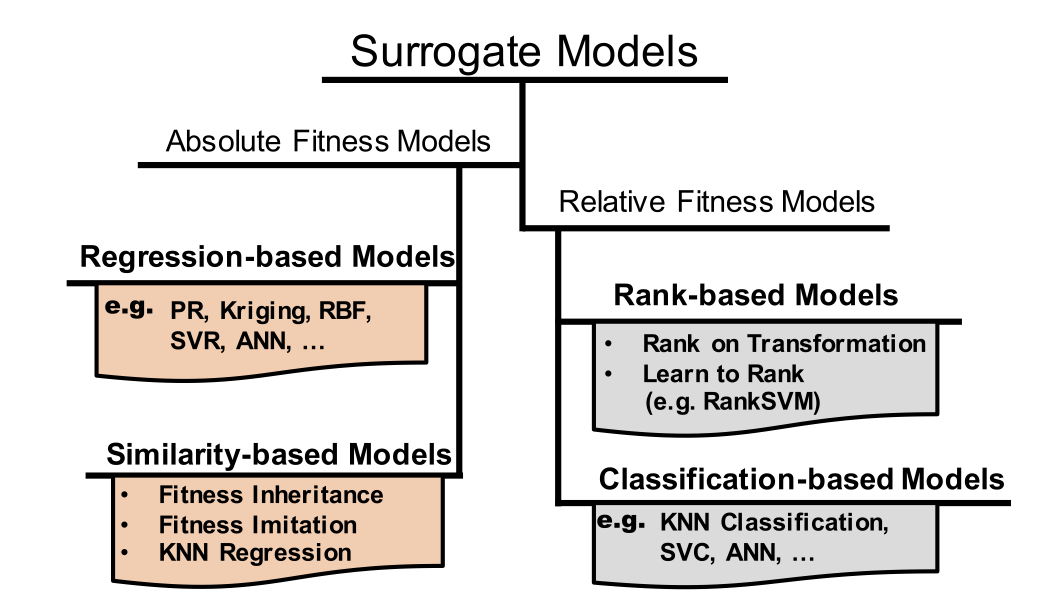
\includegraphics[width=0.7\textwidth]{./figuras/clasificacion_surrogates/clasificacion_sgs.png}
    \caption{Clasificación de las técnicas subrogadas según el tipo de predicción, adaptada de \cite{tong2021surrogate}.}
    \label{fig:clasificacion_sgs}
\end{figure}

Los modelos de \textbf{fitness absoluto} intentan estimar el valor numérico exacto de la función objetivo para una solución candidata. Bajo este enfoque, el subrogado se utiliza como una función aproximada \(\hat{f}\) capaz de asignar una predicción escalar a cada punto del espacio de búsqueda. Esta formulación coincide con el uso más clásico de los modelos subrogados, ya que permite sustituir una evaluación costosa por una predicción directa del \textit{fitness}. Dentro de esta categoría se sitúan, entre otros, los modelos basados en regresión y los métodos basados en similitud local, que estiman la calidad de una solución a partir de su relación con muestras previamente evaluadas.

Por el contrario, los modelos de \textbf{fitness relativo} no buscan reproducir el valor real de la función objetivo, sino inferir relaciones comparativas entre soluciones. En este caso, el subrogado se utiliza para estimar qué candidato es preferible, qué soluciones deberían ocupar posiciones superiores en un ranking o qué individuos pertenecen a una región prometedora del espacio de búsqueda. Este enfoque resulta especialmente relevante cuando el objetivo del optimizador no es conocer la magnitud cuantitativa de cada solución o este es difícil de estimar, sino tomar decisiones de selección, reemplazo o priorización entre candidatos, tareas que a menudo resultan menos exigentes estadísticamente que ajustar con precisión sus valores absolutos \cite{yuxue2024effective}.

Esta segunda perspectiva conecta directamente con el planteamiento experimental del presente trabajo. En una metaheurística poblacional, muchas decisiones estratégicas, como la selección de progenitores o el reemplazo de individuos, dependen del orden relativo entre soluciones más que de la magnitud exacta de sus valores de \textit{fitness}. Por ello, en el estudio de modelos orientados al fitness relativo, es de especial relevancia evaluar si el subrogado es capaz de conservar correctamente dicha estructura ordinal a lo largo de las distintas etapas de la búsqueda, lo que justifica teóricamente el uso de métricas basadas en la correlación de rangos para valorar la fidelidad cualitativa de las aproximaciones.

\subsection{Clasificación según el modo de integración}

No obstante, la utilización de técnicas subrogadas también plantea limitaciones importantes. Si el modelo aproximado no está correctamente ajustado, puede inducir al algoritmo de optimización a explorar regiones poco prometedoras del espacio, establecer un orden incorrecto entre soluciones o descartar prematuramente candidatas óptimas. Asimismo, muchos modelos presentan dificultades para generalizar fuera de las zonas en las que han sido entrenados, lo que restringe su utilidad en espacios de búsqueda amplios o con una estructura altamente no lineal \cite{forrester2009recent,bhosekar2018advances}. Por ello, la eficacia final de estos métodos depende tanto de la calidad de los datos empleados para su entrenamiento como del modo en que se integran dentro del proceso de optimización.

En función de dicha integración, la literatura distingue distintos esquemas de uso. En estrategias \textit{offline}, el modelo se entrena previamente con un conjunto de datos disponible y posteriormente se evalúa su capacidad para reproducir o anticipar el comportamiento de la función objetivo. En estrategias \textit{online}, en cambio, el subrogado se actualiza durante la propia ejecución de la metaheurística, incorporando nuevas evaluaciones reales conforme avanza la búsqueda. Dentro de esta segunda familia se sitúan enfoques como \textit{Sequential Model-Based Optimization} (SMBO), donde el modelo y la función real interactúan de forma iterativa. Por otro lado, esquemas como \textit{Predict-then-Optimise} (PtO) plantean una separación más clara entre la fase de entrenamiento del modelo y la posterior optimización sobre la aproximación construida \cite{bliek2022sustainableSBO}.

\subsubsection{Sequential Model-Based Optimization (SMBO)}
\label{subsec:smbo}

El enfoque \textit{Sequential Model-Based Optimization} se caracteriza por la alternancia iterativa entre el subrogado y la función objetivo costosa. En una primera fase se evalúa un conjunto inicial de soluciones reales con el fin de construir un conjunto de entrenamiento. A partir de esos datos se ajusta un modelo sustituto, que posteriormente se utiliza para proponer o priorizar nuevas soluciones prometedoras. Dichas soluciones son evaluadas de nuevo sobre la función real y la información obtenida se incorpora al conjunto disponible para actualizar el subrogado.

La característica distintiva de este esquema es que el modelo no sustituye definitivamente a la función objetivo, sino que se refina progresivamente a medida que avanza la búsqueda. Por ello, este tipo de integración suele asociarse a estrategias \textit{online}, en las que el subrogado actúa como un mecanismo auxiliar que orienta la exploración y reduce el número de evaluaciones reales necesarias.

\begin{figure}[H]
    \centering
    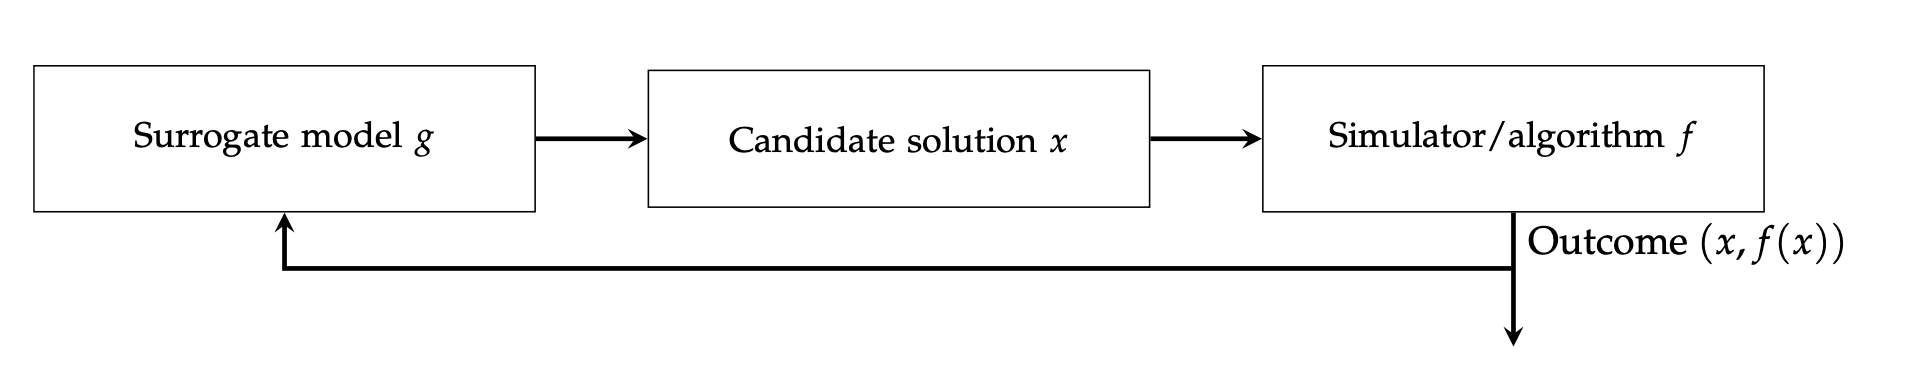
\includegraphics[width=0.95\textwidth]{./figuras/clasificacion_surrogates/smbo.png}
    \caption{Framework simplificado de un algoritmo SMBO típico obtenido de \cite{bliek2022sustainableSBO}.}
    \label{fig:smbo}
\end{figure}

La Figura~\ref{fig:smbo} muestra este ciclo de realimentación continua entre subrogado, optimización y evaluación real, donde cada nueva evaluación contribuye a mejorar la calidad del modelo.

\subsubsection{Predict-then-Optimise (PtO)}

En el enfoque \textit{Predict-then-Optimise}, el subrogado se entrena previamente a partir de un conjunto de muestras evaluadas sobre la función real y, una vez construido, pasa a utilizarse como aproximación sobre la que opera el algoritmo de búsqueda. En este caso, la fase de construcción del modelo y la fase de optimización quedan más separadas que en SMBO, ya que el modelo no se actualiza necesariamente de forma iterativa durante la búsqueda.

La principal ventaja de este esquema es que, tras el entrenamiento inicial, la optimización puede desarrollarse con un coste de evaluación mucho menor. Sin embargo, la calidad del resultado depende de la fidelidad del subrogado, ya que cualquier sesgo o error acumulado en la aproximación puede trasladarse directamente a las decisiones del optimizador. Por este motivo, PtO suele asociarse a estrategias \textit{offline} o a escenarios donde se desea estudiar previamente la capacidad del modelo para reproducir el comportamiento de la función objetivo.

\begin{figure}[H]
    \centering
    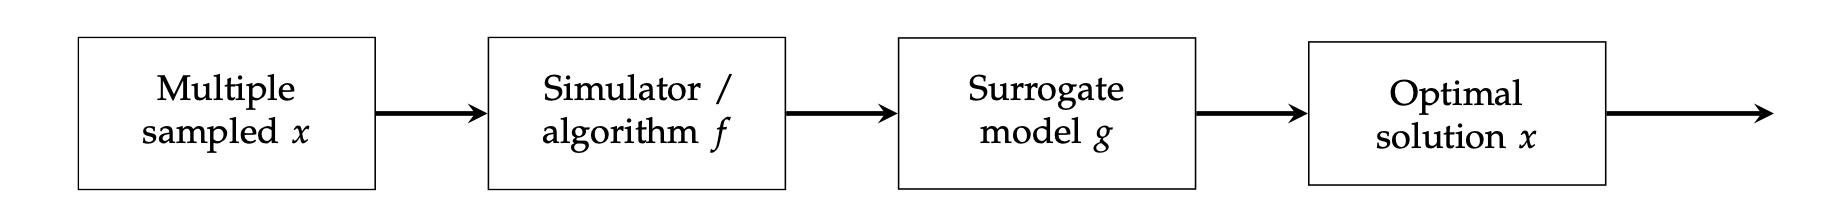
\includegraphics[width=1.00\textwidth]{./figuras/clasificacion_surrogates/pto.png}
    \caption{Framework de Predict-then-Optimise (PtO) típico obtenido de \cite{bliek2022sustainableSBO}.}
    \label{fig:pto}
\end{figure}

La Figura~\ref{fig:pto} ilustra esta separación entre la fase de construcción del subrogado y la fase posterior de optimización, sin actualización iterativa del modelo durante la búsqueda.

\subsubsection{Otras formas de integración}

Además de SMBO y PtO, existen otras formas de integración del subrogado dentro del proceso de optimización \cite{bliek2022sustainableSBO}. Algunas estrategias reutilizan información obtenida en optimizaciones previas para construir modelos aplicables a problemas futuros similares. Otras emplean el subrogado como herramienta de apoyo a la interacción humana o como aproximación de subproblemas internos en esquemas de optimización jerárquica. También pueden plantearse enfoques híbridos o mixtos, en los que el papel del modelo cambia según la fase de búsqueda o se combina con otros mecanismos de decisión.

Aunque estas variantes amplían el panorama de integración posible, en este trabajo los esquemas SMBO y PtO resultan especialmente útiles como marcos conceptuales para contextualizar los enfoques \textit{online} y \textit{offline} considerados posteriormente.





%% Concepto y taxonomía de los modelos "Surrogate" (Sustitutos)
%% Aproximaciones matemáticas y estadísticas clásicas (Kriging, RBF, RSM).
%% Diferencia operativa entre el acoplamiento offline (entrenamiento estático) y online (gestión evolutiva interactiva).

%% previamente definimos el aprendizaje automatico pero realmente queremos considerar modelos de ml como tecnicas de surrogado. deberian explicarse

%% optimización, importancia, aplicaciones...


% \section{Técnicas para la resolución de problemas de optimización}

% Debido a la relevancia práctica y teórica de los problemas de optimización, a lo largo del tiempo se ha desarrollado una amplia variedad de métodos orientados a su resolución. Estos enfoques abarcan desde procedimientos exactos y métodos matemáticos clásicos hasta técnicas aproximadas, heurísticas y metaheurísticas diseñadas para abordar problemas de elevada complejidad.

% La Figura~\ref{fig:clasificacion_tecnicas_optimizacion} resume de forma esquemática esta clasificación general.

% \begin{figure}[H]
%     \centering
%     \begin{tikzpicture}[
%             scale=0.88,
%             transform shape,
%             level distance=1.9cm,
%             sibling distance=4.3cm,
%             every node/.style={
%                     rectangle,
%                     rounded corners,
%                     draw=black,
%                     align=center,
%                     minimum width=3.0cm,
%                     minimum height=0.7cm,
%                     font=\small
%                 },
%             root/.style={
%                     fill=blue!20,
%                     font=\small\bfseries
%                 },
%             levelone/.style={
%                     fill=green!20,
%                     font=\small\bfseries
%                 },
%             leveltwo/.style={
%                     fill=orange!25,
%                     font=\small\bfseries
%                 },
%             edge from parent/.style={
%                     draw=black,
%                     thick
%                 }
%         ]

%         \node[root] {Técnicas de\\optimización}
%         child { node[levelone] {Técnicas\\exactas} }
%         child { node[levelone] {Técnicas\\aproximadas}
%                 child { node[leveltwo] {Heurísticas} }
%                 child { node[leveltwo] {Metaheurísticas} }
%             };

%     \end{tikzpicture}
%     \caption{Clasificación general de las técnicas para la resolución de problemas de optimización.}
%     \label{fig:clasificacion_tecnicas_optimizacion}
% \end{figure}


% % %% tecnicas de optimizacion

% % \begin{figure}[htbp]
% %     \centering
% %     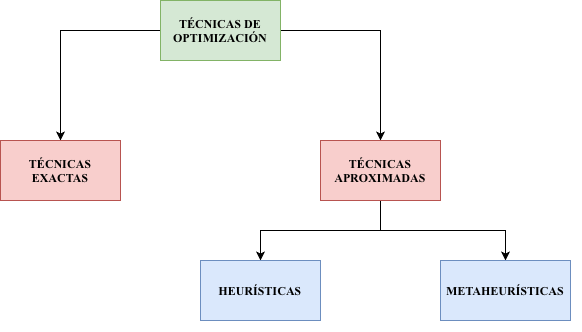
\includegraphics[width=0.85\textwidth]{./figuras/clasificacion_tecnicas_optimizacion/clasificacion_tecnicas_optimizacion.drawio.png}
% %     \caption{Clasificación general de las técnicas de optimización.}
% %     \label{fig:optimization_methods}
% % \end{figure}
% %% tecnicas exactas: garantia del optimo

% \subsection{Técnicas exactas}

% Las técnicas exactas constituyen aquellos métodos de optimización que, bajo una formulación adecuada del problema y con un presupuesto de cómputo suficiente, garantizan la obtención de la solución óptima. En este grupo se incluyen, por ejemplo, la programación lineal, la programación entera, la programación dinámica y otros procedimientos matemáticos basados en propiedades estructurales del problema.

% Su principal ventaja reside en que proporcionan garantías teóricas sobre la optimalidad de la solución obtenida. Sin embargo, esta característica suele ir acompañada de una fuerte dependencia de la formulación del problema y de un crecimiento significativo del coste computacional a medida que aumenta la complejidad del espacio de búsqueda. Por ello, cuando el problema es grande, no convexo o carece de una estructura explotable de forma directa, estas técnicas pueden resultar poco adecuadas o incluso inviables en escenarios reales.


% %% tecnicas aproximadas: sacrificio de la garantia del optimo por tiempo

% \subsection{Técnicas aproximadas}

% Aunque las técnicas exactas componen el marco de referencia desde el punto de vista teórico, en la práctica numerosos problemas de optimización deben abordarse mediante métodos aproximados capaces de proporcionar soluciones de calidad aceptable dentro de un presupuesto computacional razonable. Estas técnicas no aseguran, en general, la obtención del óptimo global, pero permiten afrontar problemas de gran escala o elevada complejidad en los que los procedimientos exactos resultan inviables por su coste o por la ausencia de una estructura suficientemente explotable \cite{boussaid2013survey}.

% El interés por este tipo de enfoques se debe a su capacidad para equilibrar calidad de solución y eficiencia temporal. Dentro de esta categoría se distinguen, de forma general, las \textbf{heurísticas} y las \textbf{metaheurísticas}, que constituyen dos de los marcos más utilizados en la optimización moderna. Aunque ambas persiguen soluciones de buena calidad en tiempos razonables, difieren en su alcance, grado de generalidad y capacidad para adaptarse a distintos problemas de optimización.

% %% heuristicas

% \subsubsection{Heurísticas}

% Generalmente, el término \textit{heurística} se utiliza para designar estrategias prácticas de resolución de problemas que permiten orientar la búsqueda de soluciones cuando no resulta viable, o no es necesario, aplicar un procedimiento exacto o exhaustivo \cite{handbookheuristics2018}. En optimización, esta idea se traduce en métodos capaces de explotar de forma eficiente la estructura del problema para obtener soluciones de calidad aceptable.

% \begin{definicion}
%     Las heurísticas son procedimientos de búsqueda orientados a obtener soluciones de buena calidad en un tiempo de cómputo reducido, sin garantizar la optimalidad de la solución obtenida.
% \end{definicion}

% Su interés radica en que permiten abordar problemas complejos en los que la resolución exacta resulta poco práctica debido al elevado coste computacional o al tamaño del espacio de búsqueda \cite{springer2024heuristics}.

% Según la forma en que generan o refinan las soluciones, las heurísticas suelen agruparse en distintas familias \cite{franca1999adaptive}. \textbf{Las heurísticas constructivas} construyen una solución desde cero, incorporando decisiones de manera progresiva hasta completar una solución factible. \textbf{Las heurísticas de mejora} parten de una solución inicial y la refinan mediante modificaciones locales orientadas a incrementar su calidad. \textbf{Las heurísticas híbridas} combinan ambos enfoques o integran estrategias adicionales de búsqueda con el objetivo de aprovechar las ventajas de cada una de ellas \cite{moreira2013hybrid}.

% %% metaheuristicas

% % - son métodos no exactos y, por lo general, no deterministas
% % - guían el proceso de búsqueda
% % - realizan una exploración eficiente del espacio de búsqueda
% % - tienen una estructura básica predefinida
% % - pueden incorporar heurísticos específicos dependientes del problema
% % - usan mecanismos para evitar regiones poco prometedoras
% % - son iterativos y disponen de criterios de parada
% % - persiguen soluciones cuasi óptimas

% % - idea: la armonización entre exploración y explotación como uno de los rasgos clave de la eficiencia de una metaheurística

% \subsubsection{Metaheurísticas}

% Las metaheurísticas constituyen una familia de métodos de optimización no exactos, diseñados para obtener soluciones de alta calidad en tiempos de cómputo razonables, especialmente en problemas complejos para los que los métodos exactos resultan inviables desde un punto de vista práctico \cite{glover1986future,talbi2009metaheuristics,boussaid2013survey}. En términos generales, se trata de procedimientos, a menudo no deterministas, concebidos para guiar de forma eficiente el proceso de búsqueda a través del espacio de soluciones \cite{talbi2009metaheuristics,luke2013essentials,marti2025fifty}.

% A diferencia de las heurísticas específicas de problema, las metaheurísticas proporcionan un marco más general de búsqueda que puede adaptarse a distintas formulaciones mediante la incorporación de operadores, reglas o mecanismos dependientes del contexto \cite{talbi2009metaheuristics,gendreau2010handbook}. Su propósito no es recorrer exhaustivamente todas las soluciones posibles, sino explorar el espacio de búsqueda de manera eficiente, favoreciendo aquellas regiones que parecen prometedoras y reduciendo el esfuerzo invertido en zonas poco rentables.

% En la mayoría de los casos, su funcionamiento se apoya en una estructura básica predefinida sobre la que se construyen mecanismos de generación, evaluación y actualización de soluciones. Este proceso se repite hasta que se satisface algún criterio de parada, como un número máximo de iteraciones, un límite temporal o una condición de convergencia \cite{luke2013essentials}. Como resultado, las metaheurísticas persiguen soluciones de calidad suficientemente alta para numerosos problemas reales, aunque sin garantizar optimalidad global \cite{glover1986future,talbi2009metaheuristics,boussaid2013survey}.

% Uno de los principios fundamentales en el diseño de metaheurísticas es el equilibrio entre exploración y explotación \cite{talbi2009metaheuristics,luke2013essentials,boussaid2013survey}. La exploración permite recorrer distintas regiones del espacio de búsqueda y reducir el riesgo de convergencia prematura, mientras que la explotación concentra el esfuerzo computacional en refinar aquellas zonas que ya han mostrado soluciones prometedoras. La capacidad para armonizar ambos comportamientos constituye uno de los elementos que más influye en la eficacia y robustez de estos métodos.


% Desde un punto de vista más abstracto, una metaheurística puede interpretarse como un esquema iterativo general compuesto por un conjunto de soluciones o estructuras de trabajo, un operador de generación de nuevas candidatas, un mecanismo de selección o reemplazo, un conjunto de variables de estado y un criterio de parada. Esta formalización, adaptada de \cite{luque2006resolucion}, permite describir bajo un mismo marco metaheurísticas de naturaleza muy distinta:
% \[
%     \mathcal{M}=\langle \Theta,\Phi,\sigma,\mu,\lambda,\Xi,\tau\rangle,
% \]
% donde \(\Theta\) es el conjunto de estructuras con las que trabaja el método, \(\Phi\) el operador que genera nuevas candidatas, \(\sigma\) la función que selecciona las estructuras que continúan en la siguiente iteración, \(\mu\) y \(\lambda\) el número de estructuras mantenidas y generadas, \(\Xi\) el conjunto de variables de estado del algoritmo y \(\tau\) el criterio de parada.

% A partir de estas características generales, las metaheurísticas pueden organizarse según distintos criterios, entre ellos el tipo de estructura sobre la que articulan la búsqueda. Esta distinción permite introducir las principales familias de métodos que se describen a continuación.

% \begin{figure}[H]
%     \centering
%     \begin{tikzpicture}[
%         node distance=0.8cm and 2.3cm,
%         every node/.style={font=\scriptsize},
%         box/.style={
%                 draw,
%                 rounded corners,
%                 align=center,
%                 minimum height=0.6cm,
%                 minimum width=2.4cm
%             },
%         rootbox/.style={
%                 box,
%                 fill=gray!15,
%                 text width=2.6cm
%             },
%         childbox/.style={
%                 box,
%                 fill=blue!8,
%                 text width=2.3cm
%             },
%         subclass/.style={
%                 box,
%                 fill=gray!3,
%                 text width=2.1cm
%             },
%         arrow/.style={
%         -{Latex[length=2mm]},
%         thick
%         }
%         ]

%         \node[rootbox] (root) {Metaheurísticas};
%         \node[childbox, below left=1.1cm and 1.5cm of root] (pop) {Basadas en\\población};
%         \node[childbox, below right=1.1cm and 0.8cm of root] (tray) {Basadas en\\trayectoria};

%         \matrix (subpops) [below=2.0cm of pop, column sep=1.8cm, row sep=0cm] {
%             \node[subclass] (enjambre) {Basadas en\\inteligencia de enjambre}; &
%             \node[subclass] (hibridas) {Híbridas};                             &
%             \node[subclass] (evolutivas) {Evolutivas};                           \\
%         };

%         \draw[arrow] (root) -- (pop);
%         \draw[arrow] (root) -- (tray);

%         \draw[arrow] (pop) -- (enjambre);
%         \draw[arrow] (pop) -- (hibridas);
%         \draw[arrow] (pop) -- (evolutivas);

%     \end{tikzpicture}
%     \caption{Clasificación general de las metaheurísticas según el tipo de estructura de búsqueda.}
%     \label{fig:clasificacion_metaheuristicas}
% \end{figure}

% \paragraph{Metaheurísticas basadas en trayectoria}

% Las metaheurísticas basadas en trayectoria se caracterizan por trabajar, en cada iteración, sobre una única solución actual o sobre un número muy reducido de soluciones estrechamente relacionadas \cite{blum2003metaheuristics,boussaid2013survey}. A partir de esa solución, el algoritmo genera nuevas candidatas mediante movimientos definidos sobre su vecindario, de modo que la búsqueda va construyendo una trayectoria a través del espacio de soluciones \cite{talbi2009metaheuristics}.

% En muchos casos, estos métodos se consideran extensiones de los procedimientos clásicos de búsqueda local. Mientras que una búsqueda local simple suele detenerse al alcanzar un óptimo local, las metaheurísticas basadas en trayectoria incorporan mecanismos adicionales para escapar de esas regiones y continuar explorando otras zonas del espacio de búsqueda \cite{gendreau2010handbook,luke2013essentials}. Entre dichos mecanismos pueden encontrarse la aceptación controlada de soluciones peores, el uso de memoria o la modificación del vecindario.

% Su principal ventaja reside en que permiten intensificar la búsqueda de manera muy eficiente alrededor de soluciones prometedoras. Sin embargo, esta misma concentración sobre una única trayectoria puede reducir la diversidad explorada y aumentar el riesgo de convergencia prematura si no se incorporan mecanismos adecuados de diversificación \cite{blum2003metaheuristics,boussaid2013survey}. Dentro de esta familia se incluyen metaheurísticas como \textit{Simulated Annealing} \cite{kirkpatrick1983optimization,vanderbilt1984monte,pedamallu2008investigating}, \textit{Tabu Search} \cite{glover1989tabu,rachid2000tabu} o \textit{Variable Neighborhood Search}. Desde la formalización abstracta introducida anteriormente, este comportamiento se corresponde típicamente con el uso de una única estructura activa por iteración, de modo que \(\mu = 1\), y con la generación de un número reducido de nuevas estructuras, por lo que \(\lambda\) suele ser pequeño.

% \paragraph{Metaheurísticas basadas en poblaciones}

% Las metaheurísticas basadas en poblaciones se caracterizan por trabajar simultáneamente con un conjunto de soluciones candidatas, en lugar de guiar la búsqueda a partir de una única solución actual \cite{blum2003metaheuristics,boussaid2013survey}. Esta característica les permite mantener activas distintas regiones del espacio de búsqueda al mismo tiempo y aprovechar la información contenida en la distribución relativa de los individuos para orientar la evolución del proceso de optimización \cite{talbi2009metaheuristics,luke2013essentials}.

% En términos generales, su funcionamiento parte de una población inicial de soluciones, a partir de la cual se generan nuevas candidatas utilizando la información disponible en los individuos ya presentes. Posteriormente, dichas soluciones se evalúan y la población se actualiza según algún criterio de selección o reemplazo \cite{talbi2009metaheuristics,boussaid2013survey}. El intercambio de información entre soluciones puede modelarse de distintas maneras, como la recombinación entre individuos, el uso de diferencias entre soluciones o la atracción hacia posiciones prometedoras.

% Una de las principales ventajas de esta familia es su elevada capacidad exploratoria. Al mantener múltiples soluciones simultáneamente, las metaheurísticas poblacionales pueden muestrear distintas zonas del espacio de búsqueda, identificar regiones prometedoras y reducir el riesgo de convergencia prematura asociado a la concentración temprana en una sola trayectoria \cite{blum2003metaheuristics,boussaid2013survey,omidvar2022review}. No obstante, esta ventaja suele ir acompañada de un mayor coste computacional por iteración, ya que en cada ciclo deben evaluarse varias soluciones candidatas. Esta observación resulta especialmente relevante en problemas con funciones objetivo costosas, donde el uso de grandes poblaciones puede hacer necesario recurrir a estrategias de aceleración, paralelización o modelado \textit{surrogate} \cite{omidvar2022review}.

% Desde la formalización abstracta introducida anteriormente, las metaheurísticas basadas en poblaciones se caracterizan por operar con varias estructuras activas en cada iteración, por lo que \(\mu > 1\). Del mismo modo, el número de nuevas estructuras generadas en cada ciclo también suele ser superior al de los métodos basados en trayectoria, de manera que \(\lambda > 1\).

% \subparagraph{Metaheurísticas poblacionales basadas en inteligencia de enjambre}

% Las metaheurísticas basadas en inteligencia de enjambre modelan comportamientos colectivos descentralizados, en los que múltiples agentes interactúan entre sí y con el entorno para orientar la búsqueda. En esta familia se sitúan, entre otros, \textit{Particle Swarm Optimization} \cite{kennedy1995pso} o \textit{Ant Colony Optimization} \cite{socha2008aco}.

% \subparagraph{Metaheurísticas poblacionales híbridas}

% Las metaheurísticas híbridas poblacionales combinan mecanismos de búsqueda poblacional con procedimientos adicionales de intensificación, como búsqueda local o estrategias meméticas, con el objetivo de combinar exploración global y refinamiento local \cite{lozano2004memetic,ong2004metalamarckian,renders1996hybrid,hart1994adaptive}. Dentro de este panorama también pueden situarse enfoques basados en modelado probabilístico, como los \textit{Estimation of Distribution Algorithms} \cite{ahn2008eda}.

% \subparagraph{Metaheurísticas poblacionales evolutivas}

% Los algoritmos evolutivos (EA) constituyen una familia de metaheurísticas poblacionales inspiradas en los mecanismos de adaptación y evolución observados en la naturaleza. De forma general, operan sobre una población de individuos que representan soluciones candidatas al problema. A lo largo del proceso de búsqueda, dicha población evoluciona mediante operadores de selección, variación y reemplazo \cite{holland1975adaptation,mitchell1998introduction,reeves2003genetic,affenzeller2009genetic}. Cada individuo recibe una valoración cuantitativa a través de una función de aptitud o \textit{fitness}, que mide la calidad de la solución representada y guía el proceso de búsqueda.

% De forma abstracta, la dinámica de un algoritmo evolutivo puede resumirse en el Algoritmo~\ref{alg:ea_general}. En primer lugar, se genera una población inicial y se evalúa su calidad. A continuación, mientras no se satisfaga el criterio de parada, se seleccionan progenitores, se aplican operadores de recombinación y mutación para generar descendencia, se evalúan los nuevos individuos y se actualiza la población mediante algún mecanismo de reemplazo. El proceso iterativo finaliza devolviendo la mejor solución encontrada.

% \begin{algorithm}[H]
%     \caption{Esquema general de un algoritmo evolutivo}
%     \label{alg:ea_general}
%     \begin{algorithmic}[1]
%         \State $P \gets \textsc{GenerarPoblacionInicial}()$
%         \State $\textsc{Evaluar}(P)$
%         \While{no se cumpla el criterio de parada}
%         \State $P' \gets \textsc{SeleccionarPadres}(P)$
%         \State $P' \gets \textsc{Recombinar}(P')$
%         \State $P' \gets \textsc{Mutar}(P')$
%         \State $\textsc{Evaluar}(P')$
%         \State $P \gets \textsc{SeleccionarNuevaPoblacion}(P, P')$
%         \EndWhile
%         \State \Return mejor solución encontrada
%     \end{algorithmic}
% \end{algorithm}

% Dentro de esta familia se incluyen distintas líneas metodológicas, entre ellas los algoritmos genéticos, las estrategias evolutivas y métodos posteriores como \textit{Differential Evolution}, que comparten el enfoque poblacional y evolutivo, aunque difieren en la forma en que generan nueva descendencia y en los operadores que emplean.

% %% no muy largo

% % por que evaluar puede ser el cuello de botella
% % por que esto limita la aplicación prácitca de metaheurísticas
% % necesidad de reducir el número de evaluaciones necesarias para alcanzar soluciones de calidad
% % técnicas surrogate como una posible solución a este problema

% %% El concepto clave: Introduce el término "Presupuesto Computacional" (Computational Budget). Explica que, en el mundo real, no tienes "infinitas evaluaciones", sino quizás solo 500 o 1000 porque cada una tarda 10 minutos.
% %% Consecuencia: Si el presupuesto es bajo, la metaheurística no puede converger. Aquí es donde los modelos surrogate salvan el día.

% \section{Diversidad, estancamiento y convergencia prematura}
% \label{sec:diversidad_estancamiento}

% Durante el proceso iterativo de una metaheurística poblacional, la búsqueda suele alternar entre fases de exploración global y de intensificación sobre regiones prometedoras del espacio de soluciones. Esta dinámica resulta esencial, ya que permite explorar distintas zonas del espacio de búsqueda y refinar progresivamente aquellas que han mostrado mejores resultados. No obstante, también puede conducir a una reducción progresiva de la diversidad poblacional, especialmente cuando los individuos comienzan a concentrarse en torno a un conjunto reducido de soluciones de alta calidad \cite{talbi2009metaheuristics,boussaid2013survey,squillero2016divergence}.

% \begin{definicion}
%     La \textbf{diversidad poblacional} hace referencia a la variedad y heterogeneidad de las soluciones candidatas presentes en la población de una metaheurística. Mantener una diversidad adecuada es crucial para evitar el estancamiento y favorecer la exploración efectiva del espacio de búsqueda.
% \end{definicion}

% En este contexto, la diversidad es un elemento fundamental para el correcto funcionamiento de las metaheurísticas basadas en población, especialmente en problemas con paisajes de búsqueda complejos, multimodales o engañosos. Una diversidad moderada-alta favorece la exploración de múltiples regiones del espacio de soluciones, reduce la probabilidad de caer rápidamente en zonas subóptimas y mantiene la capacidad del algoritmo para generar nuevas soluciones suficientemente distintas entre sí. Por el contrario, cuando la diversidad disminuye drásticamente, la población tiende a volverse cada vez más homogénea, lo que limita la eficacia de los operadores de variación y reduce la posibilidad de descubrir regiones no exploradas previamente, dando lugar al \textbf{estancamiento} \cite{omidvar2022review,squillero2016divergence,sudholt2018benefits}.

% En términos generales, puede decirse que un algoritmo entra en \textbf{estancamiento} cuando, aun continuando con su ejecución, deja de producir mejoras significativas en la calidad de las soluciones durante un número prolongado de iteraciones o evaluaciones. Este comportamiento suele aparecer cuando la población queda atrapada en una región cuya explotación adicional apenas genera progreso. Si esta concentración ocurre demasiado pronto, o incluso en torno a un óptimo local, la explotación pasa a dominar de forma excesiva sobre la exploración y la diversidad poblacional se colapsa antes de que el algoritmo haya revisado de forma suficientemente amplia otras zonas potencialmente prometedoras. En consecuencia, esta situación de \textbf{convergencia prematura} puede interpretarse como uno de los principales mecanismos que conducen al estancamiento en metaheurísticas poblacionales \cite{pandey2014premature,squillero2016divergence,sudholt2018benefits}.

% En el contexto de este trabajo, estos conceptos son muy importantes debido al uso posterior de técnicas \textit{surrogate}. Cuando la población ha convergido de forma excesiva y los individuos se vuelven prácticamente indistinguibles entre sí, la variabilidad estructural de las muestras se reduce notablemente y la capacidad del modelo para discriminar entre soluciones pierde utilidad práctica. En estas condiciones, tanto la predicción como el ranking entre candidatos tienden a aportar menos información relevante para orientar la búsqueda.

% % Para mitigar este tipo de situaciones, en la literatura resulta habitual incorporar \textbf{mecanismos de reinicio} orientados a reactivar la exploración cuando el proceso de búsqueda muestra señales claras de pérdida de diversidad o ausencia prolongada de mejora \cite{fukunaga1998restart,lozano2008replacement,luna2025elitist}. La idea general consiste en regenerar total o parcialmente la población con el fin de desplazar la búsqueda hacia nuevas regiones del espacio de soluciones. En este contexto, un \textit{reinicio aleatorio} o \textit{reinicio desde cero} regenera completamente la población, mientras que un \textit{reinicio elitista} preserva una parte de la información previamente adquirida. No obstante, un reinicio completo puede conllevar la pérdida de información valiosa acumulada durante la ejecución, especialmente cuando el algoritmo ya ha identificado soluciones de alta calidad. Por ello, en este y en muchos otros contextos resulta preferible optar por un enfoque de \textbf{reinicio elitista}, que no elimina toda la información previa, sino que preserva uno o varios de los mejores individuos encontrados hasta ese momento y regenera el resto, buscando combinar recuperación de diversidad y mantenimiento del progreso acumulado. En consecuencia, el reinicio elitista puede interpretarse como un mecanismo de control de la dinámica poblacional que busca restaurar la capacidad exploratoria del algoritmo sin renunciar completamente a la explotación de la información previamente adquirida \cite{fukunaga1998restart,lozano2008replacement,luna2025elitist}. Sobre esta base conceptual, en la Sección~\ref{subsec:metodologia_reinicio} se especifica el criterio de reinicio elitista concreto adoptado en este trabajo.

% Para mitigar este tipo de situaciones, en la literatura se utilizan \textbf{mecanismos de reinicio} encargados de reactivar la exploración cuando el proceso de búsqueda muestra señales claras de pérdida de diversidad o ausencia prolongada de mejora \cite{fukunaga1998restart,lozano2008replacement,luna2025elitist}. La idea general consiste en regenerar total o parcialmente la población con el fin de desplazar la búsqueda hacia nuevas regiones del espacio de soluciones. En este contexto, un \textit{reinicio aleatorio} o \textit{reinicio desde cero} regenera completamente la población, mientras que un \textit{reinicio elitista} preserva una parte de la información previamente adquirida.

% \section{Técnicas surrogadas}

% %% Riesgos: No olvides mencionar el error de aproximación. Si el modelo es malo, guiará a la metaheurística hacia un "óptimo falso". Esto justifica por qué necesitamos la hibridación online (para re-entrenar el modelo).

% % definicion 
% % idea general
% % familias de modelos
% % modelos principales
% % ventajas y riesgos 

% \begin{definicion}
%     Sea \(f:\mathcal{X}\rightarrow\mathbb{R}\) una función objetivo costosa de evaluar. Un \textit{surrogate model} es una función aproximada \(\hat{f}:\mathcal{X}\rightarrow\mathbb{R}\), construida a partir de un conjunto finito de muestras
%     \[
%         \mathcal{D}=\{(\mathbf{x}_i,f(\mathbf{x}_i))\}_{i=1}^{n},
%     \]
%     con el objetivo de proporcionar información útil sobre el comportamiento de \(f\) de forma computacionalmente más eficiente. En muchos casos, esta información se materializa como una función aproximada \(\hat{f}:\mathcal{X}\rightarrow\mathbb{R}\), aunque también puede adoptar otras formas orientadas a comparar, clasificar o priorizar soluciones.
% \end{definicion}

% En problemas de optimización con funciones costosas, como los basados en simulación, la evaluación repetida de la función objetivo puede suponer un coste computacional elevado o incluso prohibitivo \cite{queipo2005surrogate,forrester2009recent}. En este contexto, las técnicas surrogadas permiten sustituir parcial o temporalmente la función real por una aproximación de menor complejidad, de modo que el proceso de búsqueda pueda orientarse utilizando una representación más barata de evaluar.

% Aunque los modelos surrogados suelen plantearse como aproximaciones de la función objetivo, su utilidad en optimización no se limita necesariamente a predecir con precisión el valor numérico de \(f\). En muchos casos, resulta suficiente con que proporcionen información útil para orientar la búsqueda, por ejemplo preservando el orden relativo entre soluciones, discriminando entre candidatas prometedoras y no prometedoras o apoyando decisiones de selección sin necesidad de reproducir exactamente la función original \cite{jin2011surrogate,tong2021surrogate}.

% El interés principal de estos métodos es que permiten reutilizar la información obtenida en evaluaciones previas para guiar la búsqueda hacia regiones realmente prometedoras, manteniendo una representación útil del comportamiento del problema con un coste de evaluación mucho menor \cite{queipo2005surrogate,forrester2009recent,jin2011surrogate}. Esto resulta especialmente útil cuando cada evaluación implica ejecutar un simulador, resolver un problema físico o analizar un modelo complejo. Además, su flexibilidad hace posible adaptarlos a distintos tipos de formulaciones, desde enfoques regresivos orientados a aproximar valores hasta estrategias basadas en clasificación o en comparaciones relativas entre soluciones.

% No obstante, su utilización también plantea limitaciones importantes. Si el surrogate no está bien ajustado, puede inducir al algoritmo de optimización a explorar regiones poco prometedoras, establecer un orden incorrecto entre soluciones o descartar candidatas que en realidad serían buenas. Asimismo, muchos modelos presentan dificultades para generalizar fuera de las zonas en las que han sido entrenados, lo que restringe su utilidad en espacios de búsqueda muy amplios o con una estructura altamente no lineal \cite{forrester2009recent,bhosekar2018advances}. Por ello, la eficacia de estos métodos depende tanto de la calidad del modelo construido como del tipo de información que se pretenda extraer de él y del modo en que se integre dentro del proceso de optimización.

% En el contexto de la optimización, y en particular dentro de algoritmos evolutivos y metaheurísticos, los surrogates pueden desempeñar papeles muy distintos según el modo en que se utilicen y el tipo de información que proporcionen al algoritmo de búsqueda \cite{jin2011surrogate,tong2021surrogate}. Por ello, antes de describir los modelos utilizados comúnmente, resulta conveniente introducir una visión general de las principales taxonomías utilizadas en la literatura para clasificar este tipo de técnicas.

% \subsection{Taxonomía general de las técnicas surrogadas}

% La literatura especializada no clasifica los modelos surrogados siguiendo un único criterio, sino que suele hacerlo desde perspectivas complementarias. En algunos casos, la clasificación se centra en el papel funcional que desempeña el surrogate dentro del proceso de optimización, mientras que en otros se corresponde con el tipo de información que el modelo es capaz de predecir sobre las soluciones candidatas. Ambas perspectivas son útiles, ya que permiten entender tanto cómo se utiliza el surrogate como qué tipo de apoyo proporciona al algoritmo de búsqueda.

% \subsubsection{Integración del surrogate en la optimización}

% Una de las formas más extendidas de clasificar las técnicas surrogadas, propuesta en \cite{bliek2022sustainableSBO}, consiste en atender al modo en que el modelo sustituto se integra dentro del proceso de optimización. Desde esta perspectiva, el surrogate no se distingue únicamente por su naturaleza estadística o de aprendizaje, sino por el papel funcional que desempeña respecto de la función objetivo original y del algoritmo de búsqueda. Así, pueden distinguirse enfoques en los que el surrogate se actualiza de forma iterativa durante la optimización, otros en los que sustituye completamente a la función costosa una vez entrenado, y también estrategias en las que se reutiliza información de procesos previos o se combina con otras formas de intervención o decisión.

% Esta clasificación resulta especialmente útil porque permite diferenciar no solo cómo se construye el surrogate, sino también cuándo se consulta, qué tipo de interacción mantiene con la función real y qué grado de acoplamiento presenta con el optimizador. En consecuencia, ofrece una visión más operativa del uso de modelos sustitutos en optimización que otras taxonomías centradas exclusivamente en el tipo de modelo de regresión o clasificación empleado.

% \paragraph{Sequential Model-Based Optimization (SMBO)}

% El enfoque \textit{Sequential Model-Based Optimization} se caracteriza por la alternancia iterativa entre el surrogate y la función objetivo costosa. En una primera fase se evalúa un conjunto inicial de soluciones sobre la función real con el fin de construir un conjunto de entrenamiento. A partir de esos datos se ajusta un modelo sustituto, que posteriormente se utiliza para proponer nuevas soluciones prometedoras. Dichas soluciones son evaluadas de nuevo en la función real y la información obtenida se incorpora al conjunto de entrenamiento para actualizar el surrogate.

% La característica distintiva de este esquema es que el modelo no sustituye de forma definitiva a la función costosa, sino que se refina progresivamente a medida que avanza la búsqueda. De este modo, el surrogate actúa como un mecanismo auxiliar que orienta la exploración y reduce el número de evaluaciones reales necesarias, por lo que este tipo de métodos suele identificarse con estrategias \textit{online}.

% \begin{figure}[H]
%     \centering
%     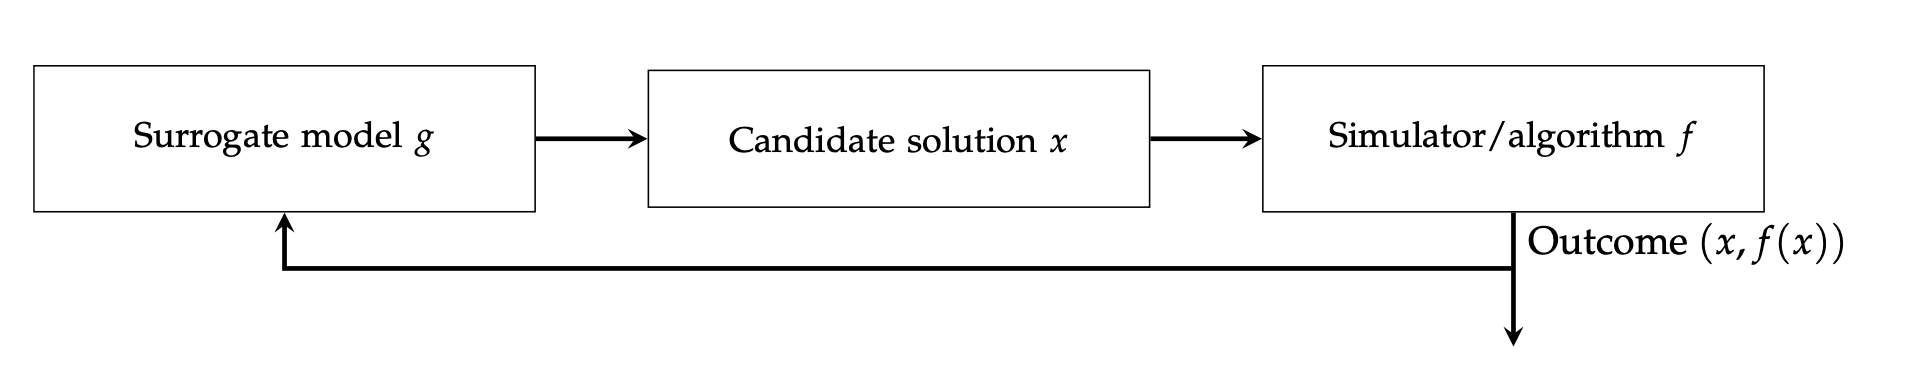
\includegraphics[width=0.95\textwidth]{./figuras/clasificacion_surrogates/smbo.png}
%     \caption{Framework simplificado de un algoritmo SMBO típico obtenido de \cite{bliek2022sustainableSBO}.}
%     \label{fig:smbo}
% \end{figure}

% La Figura~\ref{fig:smbo} muestra este ciclo de realimentación continua entre surrogate, optimización y evaluación real, donde cada nueva evaluación contribuye a mejorar la calidad del modelo.

% \paragraph{Predict-then-Optimise (PtO)}

% En el enfoque \textit{Predict-then-Optimise}, el surrogate se entrena previamente a partir de un conjunto de muestras evaluadas sobre la función real y, una vez construido, pasa a sustituir completamente a la función costosa durante la fase de optimización. En este caso, el algoritmo de búsqueda opera directamente sobre el modelo sustituto, como si éste fuese la verdadera función objetivo.

% La principal ventaja de este esquema radica en que, tras el entrenamiento inicial, la búsqueda puede desarrollarse sin recurrir continuamente a la función real, lo que reduce de forma drástica el coste computacional. Sin embargo, la calidad del resultado final depende en gran medida de la fidelidad global del surrogate, ya que cualquier sesgo o error acumulado en el modelo afectará directamente a la solución obtenida. Por este motivo, este enfoque suele asociarse a estrategias \textit{offline}.

% \begin{figure}[H]
%     \centering
%     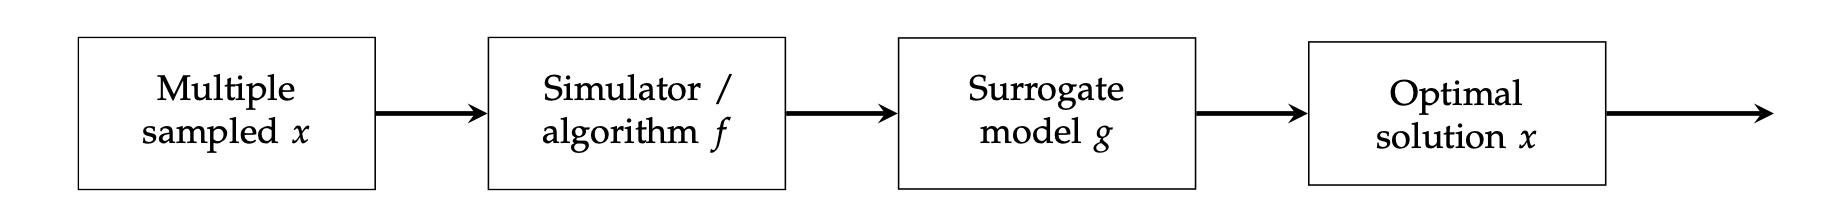
\includegraphics[width=1.00\textwidth]{./figuras/clasificacion_surrogates/pto.png}
%     \caption{Framework de Predict-then-Optimise (PtO) típico obtenido de \cite{bliek2022sustainableSBO}.}
%     \label{fig:pto}
% \end{figure}

% La Figura~\ref{fig:pto} ilustra esta separación entre la fase de construcción del surrogate y la fase posterior de optimización, sin actualización iterativa del modelo durante la búsqueda.

% \paragraph{Otras formas de integración}

% Además de los dos esquemas anteriores, la literatura recoge otras formas de integración del surrogate dentro del proceso de optimización \cite{bliek2022sustainableSBO}. El enfoque \textit{Optimise-then-Predict} (OtP) se orienta al aprovechamiento de información obtenida en optimizaciones previas para construir modelos reutilizables en problemas futuros similares. Por su parte, \textit{Predict-then-Interact} (PtI) emplea el surrogate como herramienta de apoyo a la intervención humana, de modo que el modelo no guía únicamente una optimización automática, sino también la toma de decisiones por parte del usuario.

% Asimismo, en problemas jerárquicos o anidados, los surrogates pueden utilizarse para aproximar subproblemas internos, como ocurre en ciertos esquemas de optimización bi-nivel. También existen enfoques en los que la propia construcción del surrogate se automatiza mediante procedimientos de \textit{Automated Machine Learning} o en los que se combinan varios modos de uso dentro de un mismo método, dando lugar a estrategias mixtas. Aunque estas variantes amplían el panorama de integración posible, en este trabajo resultan especialmente relevantes los esquemas SMBO y PtO, por su conexión directa con los enfoques \textit{online} y \textit{offline} considerados posteriormente.

% \paragraph{Optimise-then-Predict (OtP)}

% El enfoque \textit{Optimise-then-Predict} invierte parcialmente la lógica anterior. En este caso, primero se ejecutan procesos de optimización sobre la función costosa y, una vez obtenida información suficiente de esas ejecuciones, se construye un surrogate que permita reutilizar el conocimiento adquirido en problemas futuros similares. El modelo no se emplea necesariamente para guiar la búsqueda actual, sino como una forma de transferir experiencia de optimizaciones previas.

% Se trata, por tanto, de una categoría más amplia y menos homogénea que las anteriores, ya que incluye métodos orientados al ahorro de evaluaciones en escenarios repetitivos o familias de problemas emparentadas. Su interés reside en el aprovechamiento de información acumulada, de forma que el coste de optimización de instancias futuras pueda reducirse gracias a la experiencia acumulada.

% \begin{figure}[H]
%     \centering
%     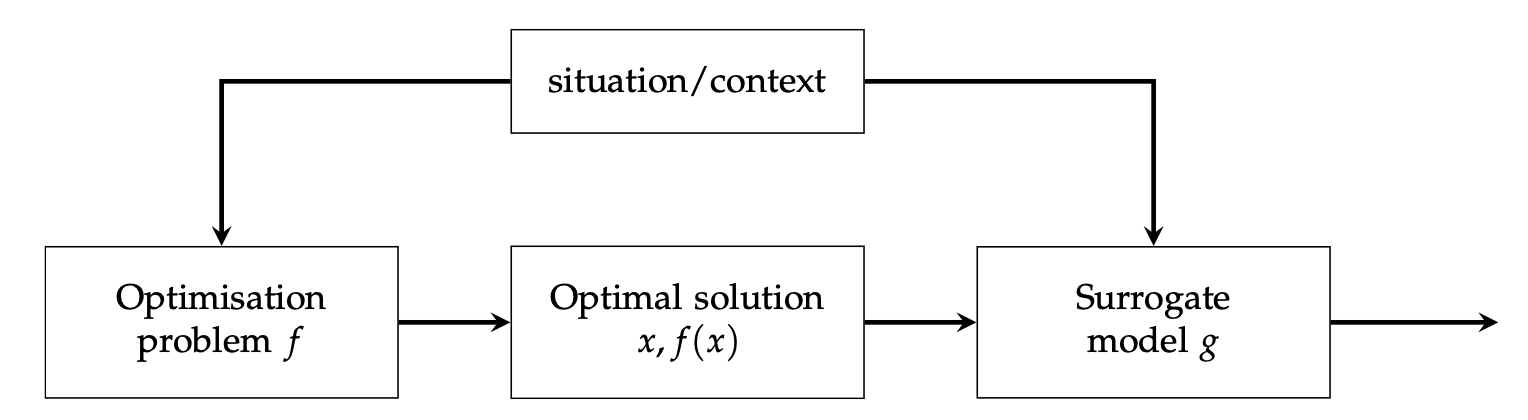
\includegraphics[width=0.95\textwidth]{./figuras/clasificacion_surrogates/otp.png}
%     \caption{Framework de Optimise-then-Predict (OtP) típico obtenido de \cite{bliek2022sustainableSBO}.}
%     \label{fig:otp}
% \end{figure}

% La Figura~\ref{fig:otp} refleja esta inversión del flujo habitual, en la que la optimización precede a la construcción del surrogate y el modelo se utiliza principalmente como mecanismo de reutilización de conocimiento.

% \paragraph{Predict-then-Interact (PtI)}

% El enfoque \textit{Predict-then-Interact} comparte con PtO la idea de construir un surrogate antes de la toma de decisiones, pero en este caso el modelo no es optimizado automáticamente por un algoritmo, sino utilizado como apoyo para la intervención humana. El usuario o experto del dominio inspecciona las predicciones del surrogate e interactúa con ellas para dirigir el proceso hacia soluciones consideradas prometedoras.

% Este esquema resulta especialmente relevante en contextos donde la experiencia humana, la interpretación del problema o la subjetividad del criterio de evaluación desempeñan un papel importante. A diferencia de los enfoques puramente automáticos, aquí el surrogate funciona como herramienta de asistencia a la decisión y no exclusivamente como sustituto computacional de la función objetivo.

% \begin{figure}[H]
%     \centering
%     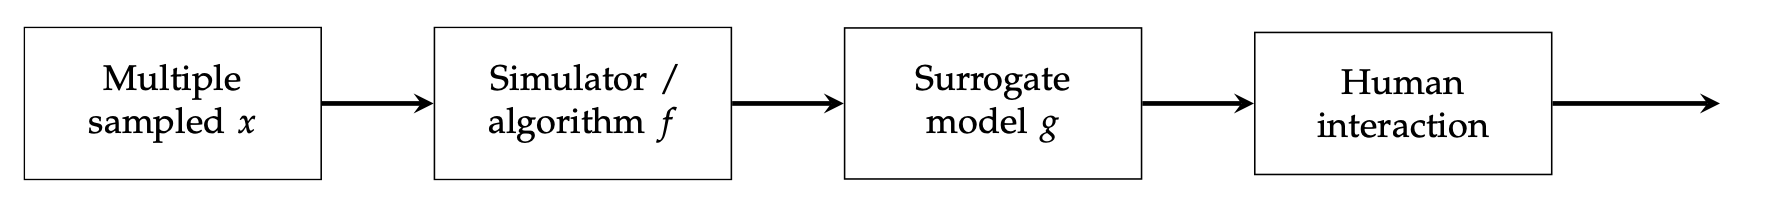
\includegraphics[width=0.95\textwidth]{./figuras/clasificacion_surrogates/pti.png}
%     \caption{Framework de Predict-then-Interact (PtI) típico obtenido de \cite{bliek2022sustainableSBO}.}
%     \label{fig:pti}
% \end{figure}

% La Figura~\ref{fig:pti} pone de manifiesto que el elemento diferencial de este enfoque no es la optimización automática del modelo, sino la interacción del usuario con las predicciones generadas para orientar el proceso de búsqueda.

% \paragraph{Bi-level Optimization (BlO)}

% La \textit{Bi-level Optimization} agrupa aquellos enfoques en los que el problema de optimización está estructurado en dos niveles jerárquicos, de modo que la solución del nivel inferior depende de las decisiones adoptadas en el nivel superior. En este contexto, el surrogate suele emplearse para aproximar el problema interno, reduciendo así el coste de resolver repetidamente dicho subproblema durante la búsqueda en el nivel externo.

% La utilidad del surrogate en este caso no proviene tanto de reemplazar la función objetivo completa, sino de simplificar una de las capas del problema.

% Esto hace que su papel sea especialmente relevante en escenarios donde la optimización anidada resulta prohibitiva desde el punto de vista computacional.

% \paragraph{Automated Machine Learning (AutoML)}

% La categoría \textit{Automated Machine Learning} incorpora los casos en los que el uso del surrogate se integra dentro de procedimientos automáticos de selección, ajuste o combinación de modelos y configuraciones. En este marco, el propio proceso de construir el surrogate puede ser objeto de optimización, de modo que la elección del modelo, sus hiperparámetros o incluso la estrategia de uso del surrogate se decidan de forma automática.

% Aunque esta categoría suele quedar parcialmente fuera del núcleo clásico de la optimización surrogate, resulta conceptualmente relevante porque enfatiza la automatización del diseño del modelo sustituto y de su integración con el algoritmo de búsqueda.

% \paragraph{Mixed Surrogate-Based}

% La categoría \textit{Mixed Surrogate-Based} engloba aquellas estrategias híbridas en las que se combinan varios de los enfoques anteriores o en las que el surrogate desempeña múltiples funciones dentro del mismo procedimiento. Por ejemplo, pueden coexistir fases \textit{online} y \textit{offline}, mecanismos de actualización adaptativa del surrogate, combinación de varios modelos o integración simultánea con distintas estrategias de decisión.

% Este tipo de enfoques mixtos refleja la tendencia reciente a diseñar procedimientos más flexibles y adaptativos, en los que el surrogate no se concibe como un componente fijo, sino como una herramienta que puede cambiar de papel según la fase de la optimización, la información disponible o el comportamiento observado durante la búsqueda. En esta línea, la combinación explícita de varios modelos surrogate ha sido propuesta en la literatura como una vía para mejorar la robustez de la aproximación frente a la dependencia de un único modelo \cite{goel2007ensemble}.

% \subsubsection{Tipo de predicción}

% Otra forma útil de clasificar los modelos surrogados se basa en la naturaleza de la información que proporcionan sobre las soluciones candidatas. Desde esta perspectiva, la diferencia fundamental no reside en el algoritmo de aprendizaje utilizado, sino en si el surrogate intenta aproximar directamente el valor numérico de la función objetivo o si, por el contrario, modela únicamente relaciones relativas entre soluciones, como su orden, preferencia o pertenencia a una determinada clase \cite{tong2021surrogate}.

% Esta distinción es crucial en optimización con surrogates, ya que condiciona tanto el diseño del modelo como su integración dentro del algoritmo evolutivo. En algunos problemas interesa aproximar con la mayor fidelidad posible la función objetivo, mientras que en otros basta con determinar qué soluciones son mejores que otras sin necesidad de conocer su fitness exacto. En este contexto, la literatura distingue entre modelos de \textit{absolute fitness} y modelos de \textit{relative fitness}, cada uno con subcategorías específicas \cite{tong2021surrogate}.

% \begin{figure}[H]
%     \centering
%     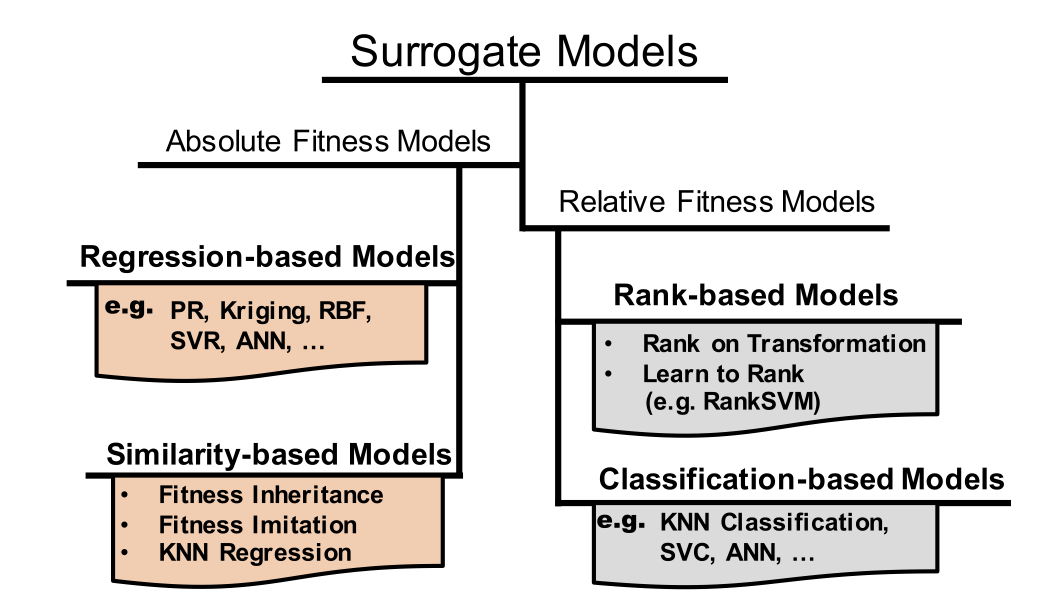
\includegraphics[width=0.7\textwidth]{./figuras/clasificacion_surrogates/clasificacion_sgs.png}
%     \caption{Clasificación de las técnicas surrogadas según el tipo de predicción, adaptada de \cite{tong2021surrogate}.}
%     \label{fig:clasificacion_sgs}
% \end{figure}

% \medskip
% \noindent\textbf{\large Modelos de fitness absoluto}\par
% \smallskip

% Los \textit{absolute fitness models} tratan de aproximar directamente el valor de la función objetivo de una solución candidata. Su propósito consiste en construir una función sustituta \(\hat{F}\) que reproduzca, con la mayor fidelidad posible, la relación entre el vector de decisión \(\mathbf{x}\) y su fitness real \(F(\mathbf{x})\). Se trata de la formulación más clásica en optimización basada en surrogates, ya que permite reemplazar evaluaciones costosas por predicciones numéricas explícitas del fitness.

% \smallskip
% \noindent\textbf{Modelos basados en regresión}\par
% \smallskip

% Dentro de los modelos de fitness absoluto, los \textit{regression-based models} constituyen la familia más común. Su objetivo es ajustar un modelo que aproxime el mapeo entre las variables de decisión y el valor escalar de fitness. Dado un conjunto de entrenamiento de la forma
% \[
%     D=\{(\mathbf{x}_1,y_1),(\mathbf{x}_2,y_2),\dots,(\mathbf{x}_n,y_n)\},
% \]
% donde \(y_i=F(\mathbf{x}_i)\), el surrogate se construye buscando minimizar la relación entre los valores reales y las predicciones del modelo.

% En esta categoría se incluyen, por ejemplo, la regresión polinómica, Kriging, las funciones de base radial, redes neuronales o métodos de ensamblado adaptados a regresión. Su ventaja principal es que proporcionan una estimación explícita del fitness, lo que permite utilizarlos directamente en operadores de selección, reemplazo o preevaluación dentro de algoritmos evolutivos.

% \smallskip
% \noindent\textbf{Modelos basados en similitud}\par
% \smallskip

% Los \textit{similarity-based models} también pertenecen a la categoría de fitness absoluto, pero estiman el fitness de nuevas soluciones a partir de su cercanía o relación con muestras previamente evaluadas. En lugar de aprender una función global explícita, estos enfoques basan la predicción en relaciones locales dentro del espacio de búsqueda. Su comportamiento depende, en gran medida, de la métrica de distancia empleada y de la distribución de las muestras disponibles.

% \medskip
% \noindent\textbf{\large Modelos de fitness relativo}\par
% \smallskip

% Los \textit{relative fitness models} no intentan predecir directamente el valor numérico de la función objetivo, sino estimar información relativa entre soluciones candidatas. En lugar de responder a la pregunta “¿cuál es el fitness de esta solución?”, estos modelos tratan de responder cuestiones como “¿qué solución es mejor?”, “¿cuál ocupa una posición más alta en el ranking?” o “¿a qué categoría de calidad pertenece esta muestra?”. Este enfoque resulta especialmente interesante en contextos donde el valor exacto del fitness es difícil de estimar o menos relevante que la capacidad de discriminar correctamente entre candidatos.

% \smallskip
% \noindent\textbf{Modelos basados en ranking}\par
% \smallskip

% Los \textit{rank-based models} constituyen una primera subcategoría dentro de los modelos de fitness relativo. Su objetivo es estimar el orden relativo de las soluciones, es decir, aprender qué candidatos deberían situarse por delante de otros en términos de calidad. En optimización evolutiva, esta aproximación puede resultar suficiente cuando el algoritmo necesita principalmente información de preferencia para seleccionar, reemplazar o priorizar individuos. Su interés radica en que, en muchos problemas, preservar correctamente el orden relativo entre soluciones puede ser más importante, y también menos costoso que ajustar con precisión sus valores absolutos \cite{yuxue2024effective}.

% \smallskip
% \noindent\textbf{Modelos basados en clasificación}\par
% \smallskip

% La segunda subcategoría de los modelos de fitness relativo es la formada por los \textit{classification-based models}. En este caso, el surrogate asigna las soluciones a distintas clases o categorías, por ejemplo distinguiendo entre individuos prometedores y no prometedores, o separando regiones de alta y baja calidad en el espacio de búsqueda. Este enfoque puede ser muy útil cuando el objetivo principal es filtrar candidatos \cite{jinglu2022classification,lin2023classification}, concentrar evaluaciones costosas en soluciones de interés o guiar el proceso de exploración.

% \section{Hibridación entre metaheurísticas y modelos surrogate}

% integración offline/online
% papel del surrogate en la busqueda de soluciones
% enfoques de hibridación offline
% ....
% enfoques de hibridación online
% surrogate como filtro de soluciones candidatas
% surrogate como guía para la generación de nuevas soluciones
% surrogate como mecanismo de selección entre operadores o estrategias de búsqueda

%%%%%

% probability-based-strategy:  probabilidad aleatoria de no usar el surrogate
% baseline strategy: se usa el surrogate en todas las evaluaciones - SIEMPRE
% candidate diversity strategy: 
% quality distance strategy: diferencia entre el fitness estimado del challenger y el fitness del challenged


% Una vez analizados los pilares conceptuales de la optimización y el modelado predictivo, se evidencia que la hibridación de algoritmos evolutivos junto con modelos de aprendizaje automático y técnicas subrogadas ofrece un marco robusto para mitigar el coste computacional. En los capítulos sucesivos se abordará cómo la literatura científica reciente ha combinado ambas disciplinas (Capítulo 4) y se detallarán las arquitecturas algorítmicas específicas, el banco de problemas CEC2017 y los modelos de regresión seleccionados como referencia para la fase experimental de este trabajo (Capítulo 5).

\chapter{Revisión de la literatura: estado del arte}
\label{chap:estado_arte}

Dentro de los algoritmos evolutivos, el uso de modelos subrogados surge como
respuesta a una limitación habitual en problemas de optimización costosa: la
evaluación repetida de la función objetivo. En este contexto, los algoritmos
evolutivos asistidos por subrogados (\textit{surrogate-assisted evolutionary
    algorithms}, SAEA) tratan de reducir el número de evaluaciones reales
necesarias mediante modelos aproximados que orientan la búsqueda hacia regiones
prometedoras.

La actividad reciente del área también se refleja en la evolución del número
de publicaciones indexadas en Scopus. La
Figura~\ref{fig:publicaciones_saea_scopus} muestra un crecimiento claro de los
trabajos relacionados con algoritmos evolutivos asistidos por subrogados
durante la última década, especialmente a partir de 2019.


\begin{figure}[H]
    \centering
    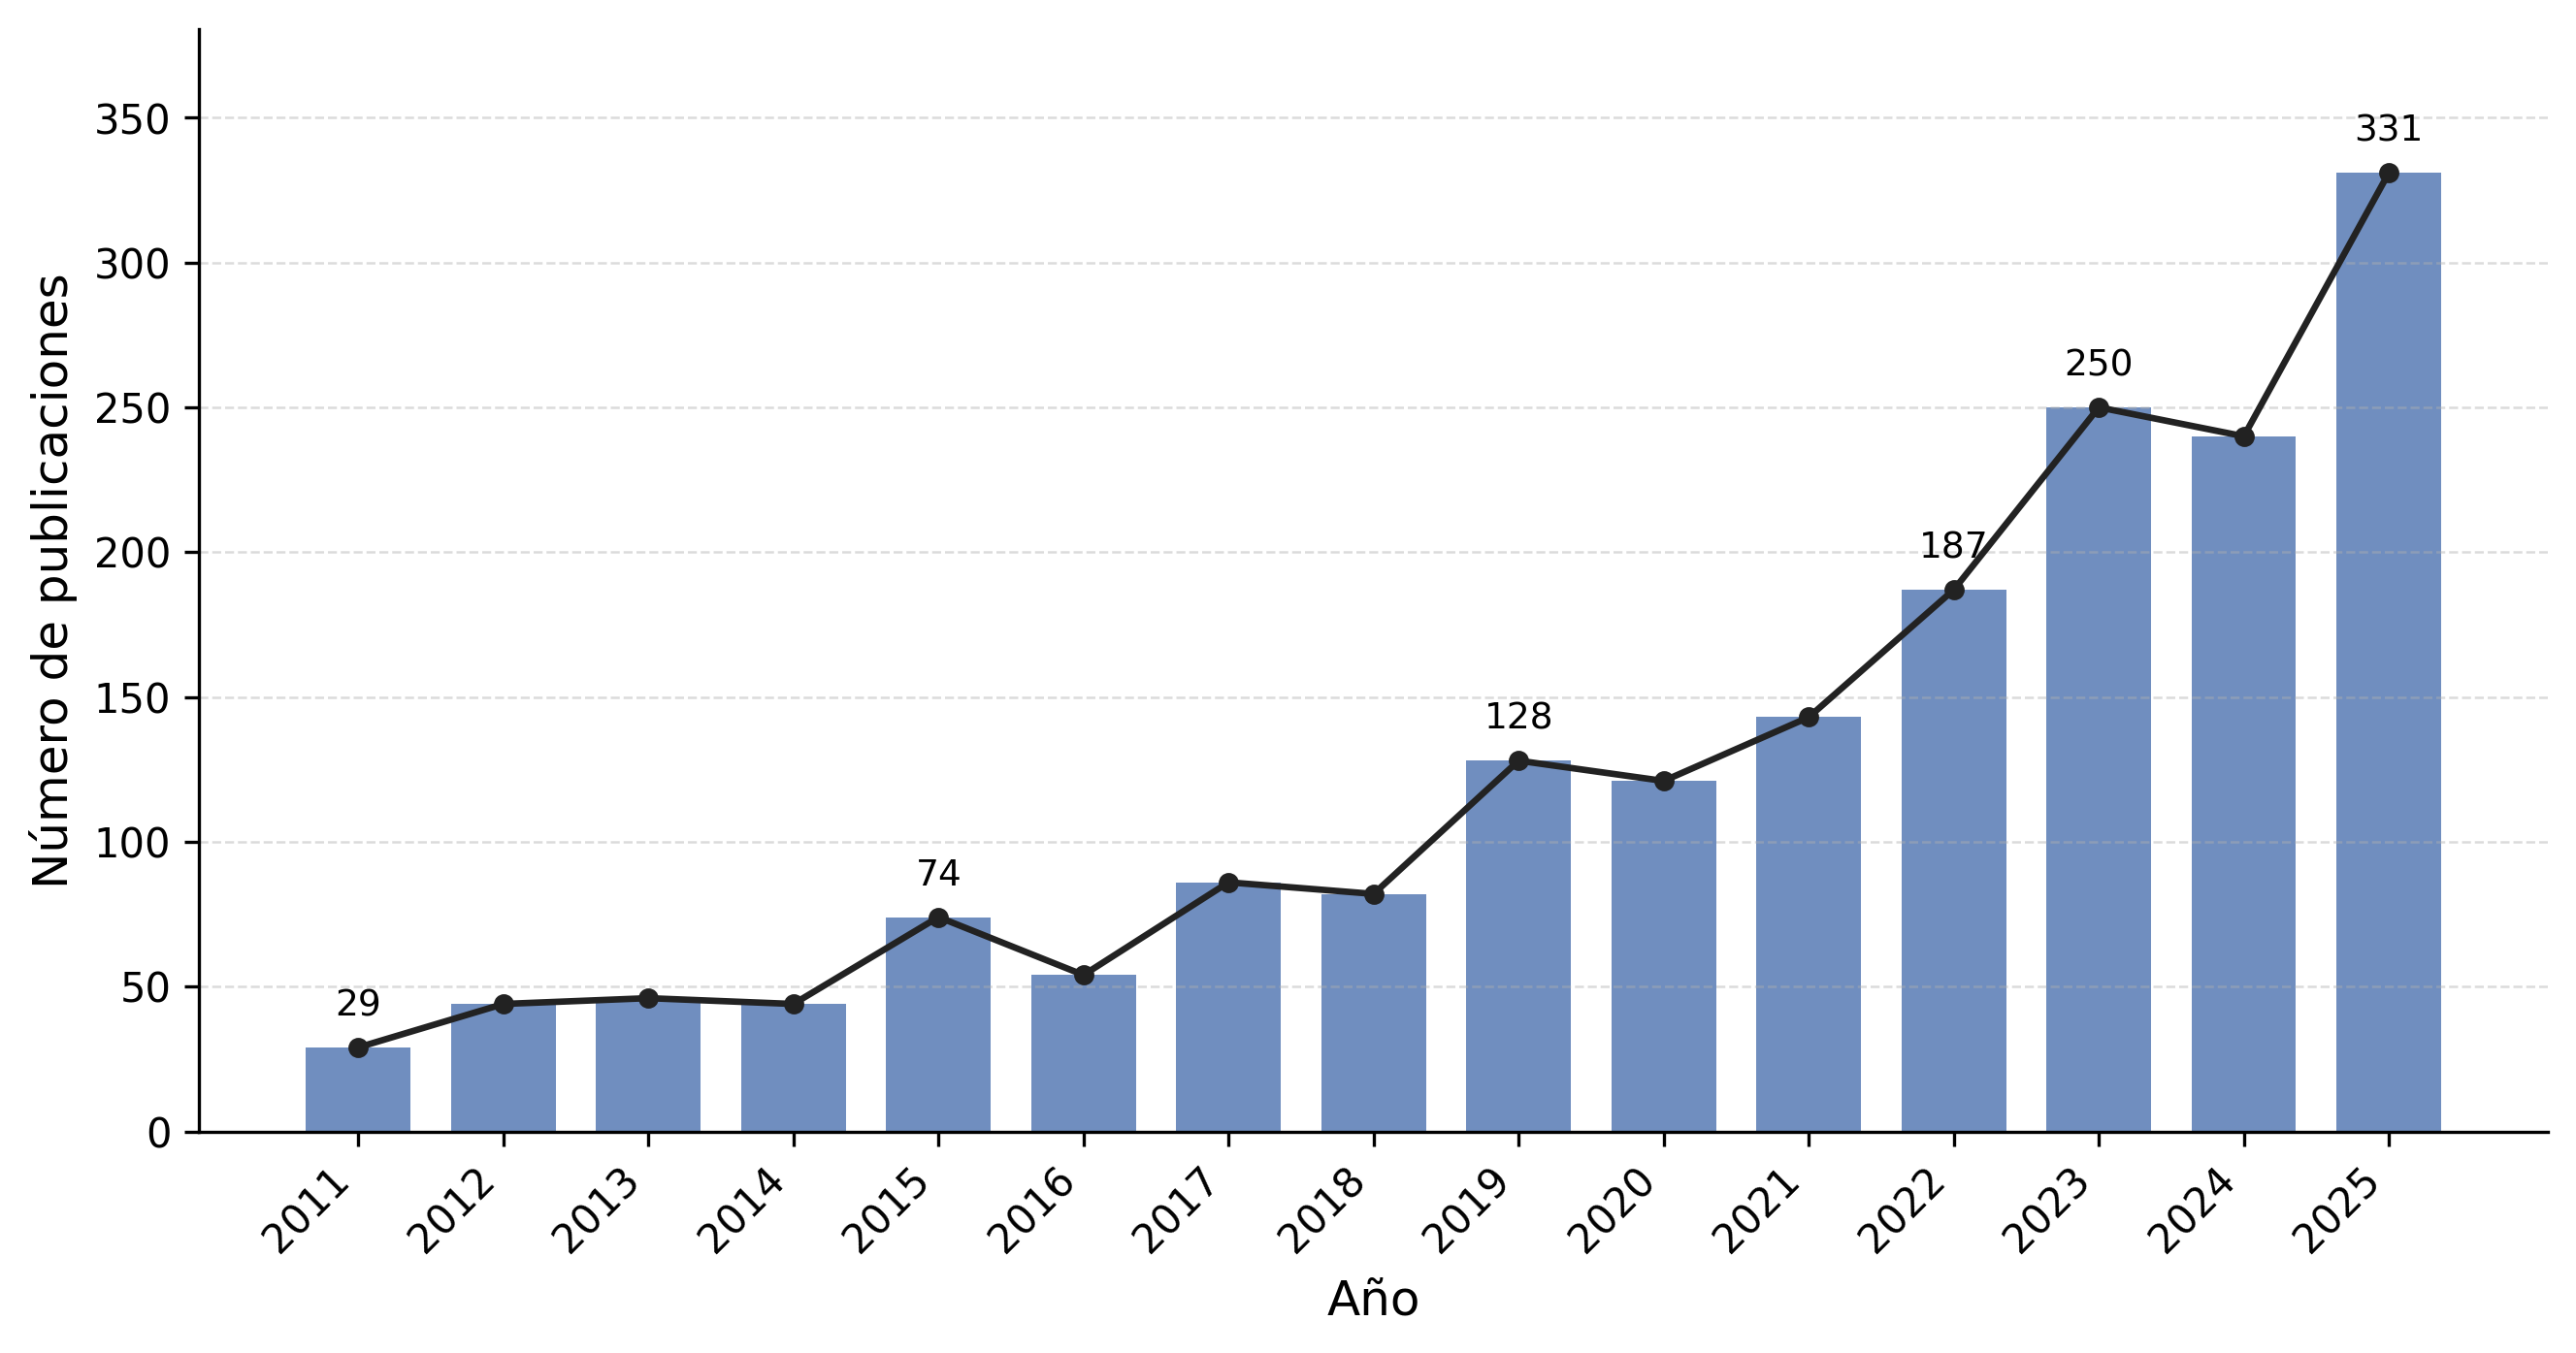
\includegraphics[width=0.85\textwidth]{figuras/estado_del_arte/publicaciones_saea_scopus.png}
    \caption{Evolución anual del número de publicaciones recuperadas en Scopus sobre algoritmos evolutivos asistidos por subrogados.}
    \label{fig:publicaciones_saea_scopus}
\end{figure}

Este capítulo sitúa la propuesta del presente trabajo dentro de esta línea de
investigación. A diferencia del capítulo anterior, centrado en los fundamentos
teóricos necesarios para comprender las técnicas empleadas, aquí el interés
recae en cómo la literatura ha abordado la integración de modelos subrogados
en algoritmos evolutivos y qué cuestiones permanecen relevantes para el diseño
experimental de este Trabajo de Fin de Grado. En particular, se presta atención
a la gestión del modelo durante la búsqueda, al tipo de información que debe
aportar el subrogado y a su integración dentro de metaheurísticas
poblacionales.  Dentro de este marco, también se considera el uso de modelos de aprendizaje automático supervisado como subrogados.

Aunque la optimización multiobjetivo asistida por subrogados constituye una
línea de investigación extensa y en auge, este trabajo se acota a la optimización
continua mono-objetivo. Esta delimitación permite centrar la revisión en los
trabajos más próximos al objetivo de esta memoria: caracterizar distintos modelos
subrogados sobre trayectorias evolutivas y estudiar posteriormente su
integración \textit{online} como mecanismo de filtrado dentro de las
metaheurísticas consideradas.

\section{Optimización evolutiva asistida por subrogados}
\label{sec:estado_saea}

El uso de modelos aproximados en optimización no es exclusivo de los
algoritmos evolutivos. Métodos como \textit{Efficient Global
    Optimization} (EGO) se apoyaron en Kriging, una técnica estadística clásica de
interpolación y modelado espacial, para guiar la búsqueda de óptimos en
funciones de caja negra costosas~\cite{jones1998}. Estas ideas sentaron una
base importante para el desarrollo posterior de la optimización basada en
subrogados dentro del cálculo computacional.

Dentro de la computación evolutiva, la incorporación de modelos subrogados se
planteó inicialmente como una forma de aproximar el \textit{fitness} de los
individuos sin evaluar siempre la función objetivo real. La revisión de
Jin~\cite{jin2005} agrupó diferentes modelos de aproximación, incluyendo
polinomios, Kriging y redes neuronales. Esta variedad refleja que los
subrogados pueden construirse tanto mediante técnicas estadísticas clásicas
como mediante modelos de aprendizaje automático supervisado. Además, este trabajo
destacó que el problema no se limita a la elección de un modelo predictivo, sino
también a decidir cómo combinar sus predicciones con evaluaciones reales para evitar que un comportamiento inadecuado del subrogado dirija la búsqueda hacia regiones incorrectas del espacio de soluciones.

A partir de estos fundamentos, años después Jin~\cite{jin2011surrogate} revisó los avances recientes de la disciplina y acotó los retos pendientes del área, entre ellos la necesidad de estrategias de gestión del modelo, el uso de varios subrogados y la falta de estudios comparativos suficientemente sistemáticos. Estos trabajos consolidan una una idea que sigue siendo crucial en la literatura actual: el subrogado no debe entenderse como un sustituto directo y permanente de la función objetivo, sino como un componente dinámico que debe ser controlado y gestionado durante el proceso evolutivo.

Las revisiones más recientes confirman la consolidación de esta línea de
investigación. He et al.~\cite{he2023review} revisan los SAEA para problemas
de optimización costosa y los organizan atendiendo tanto a los algoritmos
empleados como a sus escenarios de aplicación. Por su parte, trabajos recientes como el de Liang et al.~\cite{liang2025survey}, proponen taxonomías y esquemas generales actualiazados para describir la construcción del subrogado, su actualización y su uso dentro del algoritmo evolutivo. En conjunto, estas revisiones muestran que la integración de subrogados ha pasado de ser una técnica auxiliar a constituir una línea de investigación propia y robusta dentro de la optimización evolutiva.

\section{Gestión del modelo subrogado durante la búsqueda}
\label{sec:estado_gestion_modelo}

Uno de los aspectos más importantes en los SAEA es la forma en que se
controla la intervención del modelo subrogado durante la búsqueda. Si el
modelo se utiliza sin una política de control adecuada, sus errores pueden acumularse y
desviar al algoritmo hacia regiones que parecen prometedoras según la
aproximación, pero que no lo son al evaluarse mediante la función objetivo
real. Por este motivo, buena parte de la literatura no se centra únicamente en
mejorar la precisión del modelo, sino en diseñar mecanismos que regulen cuándo
debe intervenir y cuándo es necesario recurrir de nuevo a evaluaciones reales.

Esta idea aparece ya en el marco propuesto por Jin et al.~\cite{jin2002framework},
donde se introducen estrategias de \textit{evolution control} para combinar
evaluaciones aproximadas y reales dentro del algoritmo evolutivo. En términos
generales, estas estrategias pueden actuar a nivel de individuo, decidiendo qué
soluciones concretas se evalúan con el modelo o con la función real, o a nivel
de generación, alternando fases en las que la población se evalúa de forma
aproximada con fases de corrección mediante evaluaciones reales. Esta distinción resulta relevante porque desplaza el problema desde la elección
del modelo hacia la definición de una política de control que determine cuándo
usar la aproximación, cuándo recurrir a evaluaciones reales y a qué nivel de la
población aplicar cada decisión.

Esta gestión también afecta al tiempo durante el cual un modelo permanece
activo antes de ser actualizado. Loshchilov et
al.~\cite{loshchilov2012selfAdaptiveCMAES} propusieron una variante de CMA-ES
asistida por subrogados que ajusta \textit{online} la vida útil del modelo y
sus hiperparámetros. Aunque se trata de una metaheurística distinta a las
consideradas en esta memoria, el trabajo ilustra que la frecuencia de
actualización del subrogado forma parte del propio diseño de la integración, y
no solo de la elección del modelo predictivo.

La necesidad de controlar el modelo se ha mantenido en propuestas posteriores.
Por ejemplo, Yu et al.~\cite{yu2019restart} propusieron una estrategia de
reinicio por generaciones para un algoritmo de enjambre de partículas asistido
por un modelo RBF global. Su propuesta integra el reinicio con mecanismos de
gestión del modelo a nivel de generación y de individuo, mostrando que la
coordinación entre la dinámica de la población y el uso del subrogado puede
mejorar la búsqueda en problemas computacionalmente costosos. Este tipo de
trabajos resulta relevante para el presente Trabajo de Fin de Grado, donde se
estudia en capítulos posteriores la conveniencia de incorporar mecanismos de
reinicio en las metaheurísticas consideradas. En ese escenario, puede esperarse
que un cambio brusco en la población afecte también a la representatividad de
las muestras utilizadas para entrenar el modelo, por lo que la intervención del
subrogado debe tratarse con cautela.

Otro aspecto relacionado con la gestión del modelo es su coste computacional.
Aunque los subrogados se introducen para reducir el uso de evaluaciones reales,
su entrenamiento y predicción también consumen recursos.
Bliek~\cite{bliek2022sustainableSBO} remarca esta cuestión: no basta con
reducir el número de evaluaciones costosas, sino que debe considerarse el coste
total del proceso, incluyendo el aprendizaje del modelo y la propia
optimización sobre la aproximación. Esta observación es especialmente
importante cuando se comparan modelos de distinta complejidad, ya que una
mejora predictiva puede no compensar si introduce un coste adicional elevado.

En conjunto, estos trabajos muestran que la integración de un subrogado dentro
de una metaheurística requiere decisiones adicionales al propio modelo
predictivo. Es necesario determinar con qué datos se entrena, cuándo se
actualiza, con qué frecuencia se consulta y cómo se evita que sus errores
condicionen de forma excesiva la búsqueda.

\section{Modelos subrogados y criterios de decisión}
\label{sec:estado_modelos_informacion}

La elección del modelo subrogado no depende únicamente de su familia
estadística o de aprendizaje, sino también del tipo de información que se
espera obtener de él. En algunos enfoques, el objetivo principal es aproximar
con la mayor precisión posible el valor numérico de la función objetivo. En
otros, basta con que el modelo permita comparar soluciones, identificar
candidatos prometedores o descartar aquellos que difícilmente mejorarán la
población. Esta diferencia es especialmente relevante en algoritmos
evolutivos, donde muchas decisiones se basan en relaciones de preferencia
entre individuos más que en el valor exacto del \textit{fitness}.

%% random forest, mlps, svr...

Esta cuestión ha sido estudiada de forma explícita por Tong et
al.~\cite{tong2021surrogate}, cuyo trabajo se tomó como referencia en el
Capítulo~\ref{chap:fundamentos_teoricos} para distinguir entre modelos
orientados al \textit{fitness} absoluto y modelos orientados al
\textit{fitness} relativo. Más allá de la taxonomía, su estudio experimental
resulta relevante porque compara modelos de distinta naturaleza, como RBF,
kNN-R, RankSVM y SVC, atendiendo no solo a la calidad predictiva, sino también
al coste de construcción y predicción y a su efecto dentro de un SAEA
mono-objetivo.

De forma complementaria, Díaz-Manríquez et
al.~\cite{diaz2017metamodeling} compararon distintas técnicas subrogadas
integradas en algoritmos evolutivos, incluyendo superficies de respuesta
polinómicas, Kriging, RBF y SVR. Su análisis resulta especialmente útil en este
contexto porque no se limita a medir la precisión de las predicciones, sino que
también considera la preservación del ranking como indicador para seleccionar
modelos adecuados dentro de un proceso evolutivo. Esta conclusión refuerza la
necesidad de valorar los subrogados no solo por su error numérico, sino también
por su capacidad para mantener relaciones de orden entre soluciones candidatas.

La incorporación de técnicas de aprendizaje automático amplía este marco más
allá de los modelos estadísticos clásicos. Naharro et
al.~\cite{naharro2022regressionPairwise} comparan formulaciones basadas en
regresión, orientadas a aproximar el \textit{fitness}, con modelos pareados
que tratan directamente la comparación entre soluciones. Su estudio considera
distintos algoritmos de aprendizaje automático, incluyendo regresión
regularizada, redes neuronales, árboles de decisión, métodos de \textit{boosting}
y bosques aleatorios. Este tipo de análisis resulta útil para este trabajo
porque muestra que la utilidad de un subrogado no depende únicamente del modelo
empleado, sino también de cómo se incorporan sus predicciones dentro del
proceso de optimización.

Algunos trabajos llevan esta idea hacia modelos de clasificación, donde el
subrogado separa soluciones prometedoras y no prometedoras. Sin embargo, el presente
Trabajo de Fin de Grado se mantiene en el ámbito de modelos regresivos, ya que
cada solución candidata tiene asociado un valor real de \textit{fitness}.

Esta distinción entre aproximar valores y apoyar decisiones justifica que la
evaluación de modelos subrogados no se limite a métricas de error absoluto.
Cuando el subrogado se utiliza dentro de una metaheurística para decidir qué
candidatos merecen una evaluación real, resulta esencial medir también si
mantiene correctamente las relaciones de orden entre soluciones. Por este
motivo, en el presente Trabajo de Fin de Grado se consideran métricas de error
junto con métricas ordinales, de forma que la selección del modelo tenga en
cuenta tanto la precisión numérica como su utilidad potencial dentro del
proceso de optimización.

\section{Integración de subrogados en metaheurísticas poblacionales}
\label{sec:estado_integracion_metaheuristicas}

La integración de un subrogado dentro de una metaheurística poblacional no se
limita a entrenar un modelo externo y consultar sus predicciones. En la mayoría
de propuestas recientes, el modelo se incorpora dentro de decisiones concretas
del algoritmo, como la selección de descendientes, la identificación de regiones
prometedoras o la elección de muestras que deben evaluarse mediante la función
objetivo real. Por ello, el rendimiento final depende tanto de la calidad del
modelo como del modo en que sus predicciones modifican la dinámica de la
población.

Dentro de los SAEA recientes, la evolución diferencial aparece con frecuencia
como base algorítmica para integrar subrogados en problemas continuos. Wang et
al.~\cite{wang2019evolutionarySampling} siguen esta idea en ESAO, donde un
modelo RBF global se utiliza para preseleccionar descendientes generados por
evolución diferencial, mientras que una búsqueda local asistida por subrogado
refuerza la explotación de regiones prometedoras.

Otros trabajos han extendido esta integración mediante estructuras más
elaboradas. Cai et al.~\cite{cai2020generalizedSAEA} propusieron un algoritmo evolutivo asistido por subrogados para problemas costosos de alta dimensión, basado en un marco de algoritmo genético que combina búsqueda local mediante subrogado, actualización guiada de la población y preselección de candidatos mediante un criterio de mejora esperada. Asimismo, Wang et al.~\cite{wang2023glsade} combinaron un modelo RBF global y un modelo Kriging local dentro de una evolución diferencial asistida por subrogados, utilizando el primero para capturar tendencias globales y el segundo para explotar regiones prometedoras teniendo en cuenta la incertidumbre del modelo. Estas propuestas muestran que el subrogado no se emplea únicamente para aproximar el \textit{fitness}, sino también para regular de forma adaptativa qué zonas del espacio de búsqueda reciben nuevas evaluaciones reales.

La frecuencia y el modo de actualización del modelo durante la búsqueda también constituyen un reto crítico en los enfoques \textit{online}, dado que el reentrenamiento continuo de un aproximador conforme se acumulan datos puede convertirse en un cuello de botella computacional. Para mitigar este impacto, trabajos como el de Zhan y Xing~\cite{zhan2021fastKriging} exploran el uso de esquemas de aprendizaje incremental orientados específicamente a reducir el coste de reconstrucción del subrogado a lo largo de las iteraciones. Esta preocupación por la eficiencia temporal es un factor clave en el presente Trabajo de Fin de Grado, donde la viabilidad de la integración \textit{online} de los modelos de aprendizaje automático considerados depende directamente de mantener un coste de computación contenido.

La presencia destacada de la evolución diferencial en esta línea de investigación ha dado lugar incluso a revisiones específicas, como la de Yu et al.~\cite{yu2025sade}, centrada exclusivamente en el análisis de algoritmos de evolución diferencial asistidos por subrogados. Esta tendencia justifica que parte de la comparación experimental del presente trabajo se realice sobre DE y SHADE, dos algoritmos directamente relacionados con esta familia. No obstante, el objetivo de esta memoria no es proponer una variante específica de evolución diferencial, sino evaluar si un modelo subrogado seleccionado mediante una fase \textit{offline} puede integrarse bajo un protocolo común como filtro \textit{online} en metaheurísticas poblacionales de distinta naturaleza, incluyendo también un algoritmo genético.

\section{Posicionamiento del presente trabajo}
\label{sec:estado_posicionamiento}

La literatura revisada muestra que la utilidad de un modelo subrogado en
optimización evolutiva no depende únicamente de su precisión predictiva. Su
efecto final está condicionado por el tipo de información que aporta, por el
coste de construirlo y actualizarlo, y por la forma concreta en que sus
predicciones intervienen dentro del algoritmo evolutivo. Esta perspectiva
motiva que el presente trabajo no plantee la selección del subrogado como una
comparación aislada entre modelos, sino como una evaluación progresiva:
caracterizar primero varios modelos subrogados sobre trayectorias evolutivas ya
generadas y, a partir de esa evidencia, estudiar posteriormente su integración
\textit{online} dentro de las metaheurísticas consideradas.

Aunque existen trabajos sobre optimización evolutiva basada en datos
históricos, revisados de forma general por Jin et
al.~\cite{jin2019datadriven}, el uso \textit{offline} realizado en esta memoria
tiene un propósito distinto. En este caso, el subrogado no se emplea para
ejecutar la búsqueda, sino para caracterizar modelos sobre trayectorias ya
generadas antes de integrarlos posteriormente en el bucle de optimización.

A partir de esa caracterización, la integración \textit{online} se aborda como
un mecanismo de filtrado controlado. El subrogado no sustituye de forma
definitiva a la función objetivo, sino que decide qué candidatos parecen lo
suficientemente prometedores como para consumir una evaluación real. De este
modo, el trabajo se sitúa en la línea de los SAEA que combinan predicción,
gestión del modelo y evaluación real, analizando hasta qué punto una misma
estrategia de integración puede aplicarse de forma robusta a distintas
metaheurísticas poblacionales consideradas en la memoria.

Los capítulos siguientes presentan las metaheurísticas, los modelos, las estrategias de evaluación y el marco experimental utilizados.


\chapter{Algoritmos y técnicas de referencia}
\label{chap:algo_tecnicas_ref}

%% que se compara

En este capítulo se presentan los algoritmos y técnicas que servirán como base para el desarrollo experimental del trabajo. En primer lugar, se describen las metaheurísticas consideradas como algoritmos de referencia, prestando atención a su funcionamiento general, sus operadores principales y el papel que desempeñan en la generación de trayectorias de búsqueda. A continuación, se introduce la estrategia de reinicio de población empleada para mitigar situaciones de estancamiento y favorecer la recuperación de diversidad durante la optimización.

Además de los algoritmos de búsqueda, el capítulo recoge los modelos utilizados como técnicas subrogadas, diferenciando entre los modelos de aprendizaje automático considerados en la comparativa principal y las técnicas subrogadas clásicas que podrán emplearse posteriormente como referencia. Los fundamentos generales de las metaheurísticas, el aprendizaje automático y los modelos subrogados ya fueron presentados en el Capítulo~\ref{chap:fundamentos_teoricos}. Por tanto, aquí se adopta una perspectiva más operativa, centrada en los componentes concretos utilizados en el estudio. Finalmente, se definen las estrategias \textit{offline} utilizadas para evaluar los modelos sobre trayectorias previamente generadas y se presenta el esquema \textit{online} mediante el que el subrogado se integrará posteriormente dentro del bucle de optimización. La finalidad de este capítulo no es analizar todavía el rendimiento de las técnicas, sino fijar con claridad qué componentes intervienen en el estudio y cómo se relacionan con la fase experimental presentada en los capítulos posteriores.


\section{Metaheurísticas consideradas}

Las metaheurísticas consideradas en este trabajo constituyen las herramientas de búsqueda empleadas para generar las trayectorias de optimización que posteriormente serán utilizadas para el análisis de técnicas subrogadas. Todas ellas trabajan sobre soluciones representadas mediante vectores reales dentro del dominio de búsqueda y siguen una dinámica poblacional, en la que un conjunto de individuos evoluciona mediante operadores de generación, evaluación y reemplazo.

La elección de \textbf{AGE}, \textbf{DE} y \textbf{SHADE} permite cubrir distintos niveles de complejidad y adaptación dentro de la optimización evolutiva:

\begin{itemize}
    \item \textbf{AGE} actúa como una referencia genética sencilla basada en reemplazo estacionario,
    \item \textbf{DE} proporciona una referencia robusta y ampliamente utilizada en optimización continua,
    \item \textbf{SHADE} extiende la evolución diferencial (DE) mediante un esquema adaptativo que ajusta dinámicamente sus parámetros de control.
\end{itemize}

De este modo, las trayectorias obtenidas permiten estudiar cómo varía la utilidad de los modelos subrogados en función de la dinámica de búsqueda que genera los datos. Al mismo tiempo, hacen posible comparar esquemas evolutivos con distintos mecanismos de generación y adaptación.

%% herramientas de busqueda

%% que es
%% por que se usa
%% como funciona a nivel operativo
%% papel despues en los experimentos

%% 1. motivacion y papel en el trabajo: por que se incluye
%     - algoritmo base
%     - referencia evolutiva
%     - comparacion entre familias, etc...
% 2. representación de la solución: individuos como vectores reales 
% 3. funcionamiento general: describir el ciclo:
%     - inicializacion
%     - evaluacion
%     - generacion de candidatos
%     - selecction/reemplazo y parada
% 4. operadores principales:
%     - AGE: 
%         - seleccion, cruce, mutacion, reemplazo estacionario
%     - DE: 
%         - mutacion diferencial, cruce binomial, seleccion greedy
%     - SHADE: 
%         - memoria histórica de parámetros, adaptacion de F y CR
% 5. pseudocodigo
% 6. relacion con el resto del tfg


% --------

% %% soporte visual:

% - pseudocodigo para cada metaheurística compacto
% - formulas principales de operadores: mutacion, cruce, selección
% - esquema del reinicio de población


\subsection{Algoritmo Genético Estacionario (AGE)}

Los algoritmos genéticos (\textbf{AG}) constituyen uno de los enfoques clásicos y más conocidos dentro de las metaheurísticas evolutivas descritas en la Sección~\ref{subsec:mh_evolutivas}. Sus fundamentos modernos fueron consolidados  en 1975 y posteriormente difundidos y sistematizados por Goldberg \cite{goldberg1989genetic}. Estos algoritmos se basan en mantener una población de soluciones candidatas y generar nuevos individuos mediante operadores inspirados en la evolución biológica, principalmente la selección de progenitores, el cruce y la mutación.

Dentro de esta familia, el \textbf{Algoritmo Genético Estacionario} o, según sus siglas, \textbf{AGE}, se caracteriza por actualizar la población de forma parcial y progresiva. Uno de los antecedentes clásicos de este enfoque es GENITOR, analizado por L. Darrell Whitley en 1989 \cite{whitley1989stationary}. A diferencia de un algoritmo genético generacional (AGG), donde la población se reemplaza de forma completa o casi completa en cada generación, en un esquema estacionario la descendencia generada compite con los individuos ya presentes en la población. Esta actualización parcial y gradual de la población permite conservar parte de la estructura poblacional previa e incorporar nuevas soluciones únicamente cuando mejoran la calidad del conjunto. A pesar de dichas diferencias, las fases de un \textbf{AG} se mantienen.

En este trabajo, AGE se incluye como una referencia evolutiva sencilla frente a métodos diferenciales más especializados como DE y SHADE. Su utilización permite generar trayectorias basadas en operadores genéticos clásicos y analizar posteriormente si la utilidad de los modelos subrogados depende de la dinámica poblacional que produce los datos.

Formalmente, cada individuo se representa mediante un vector real
\(\mathbf{x}_i \in \mathbb{R}^D\), donde cada componente corresponde a una
variable de decisión del problema de optimización continua. El
Algoritmo~\ref{alg:age} recoge el pseudocódigo de la variante concreta de AGE utilizada en este trabajo. Aunque el esquema sigue siendo el de un algoritmo genético estacionario, el pseudocódigo fija las decisiones concretas empleadas en este trabajo, como los operadores utilizados sobre vectores reales y el criterio de reemplazo de la población.


%% tenemos que revisar las memorias sueprvisads por daniel ya que en la mayoria se plantea algo de contexto previo al algoritmo, es deicr, antes de justificar por que lo utilizamos. 

\begin{algorithm}[H]
    \begin{algorithmic}[1]
        \State $P \gets \textsc{GenerarPoblacionInicial}()$
        \State $\textsc{Evaluar}(P)$
        \While{no se cumpla el criterio de parada}
        \State $p_1, p_2 \gets \textsc{SeleccionTorneo}(P)$
        \If{$\operatorname{rand}() < p_c$}
        \State $h_1, h_2 \gets \textsc{CruceBLX\_alpha}(p_1, p_2)$
        \Else
        \State $h_1 \gets p_1$
        \State $h_2 \gets p_2$
        \EndIf
        \State $h_1 \gets \textsc{MutacionGaussiana}(h_1, p_m, \sigma)$
        \State $h_2 \gets \textsc{MutacionGaussiana}(h_2, p_m, \sigma)$
        \State $\textsc{Evaluar}(h_1, h_2)$
        \State $h^\star \gets \textsc{SeleccionarMejorHijo}(h_1, h_2)$
        \State $P \gets \textsc{ReemplazoEstacionario}(P, h^\star)$
        \EndWhile
        \State \Return mejor solución encontrada
    \end{algorithmic}
    \caption{Algoritmo Genético Estacionario (AGE).}
    \label{alg:age}
\end{algorithm}

El flujo general descrito en el Algoritmo~\ref{alg:age} se representa esquemáticamente en la Figura~\ref{fig:flujo_age}. A partir de la población actual, AGE selecciona dos progenitores, genera descendencia mediante cruce y mutación, evalúa los nuevos individuos y actualiza parcialmente la población mediante un mecanismo de reemplazo estacionario.

En las siguientes subsecciones se detallan los operadores concretos empleados en este trabajo.

% \begin{figure}[H]
%     \centering
%     \includegraphics[width=0.95\textwidth]{figuras/algoritmos/flujo_age.png}
%     \caption{Esquema general del funcionamiento de un algoritmo genético estacionario.}
%     \label{fig:flujo_age}
% \end{figure}



\begin{figure}[H]
    \centering
    \begin{adjustbox}{max width=\textwidth}
        \begin{tikzpicture}[
            node distance=2.5cm and 6.5cm,
            box/.style={
                    draw=black,
                    fill=white,
                    rectangle,
                    line width=0.8pt,
                    minimum width=3.8cm,
                    minimum height=1.6cm,
                    align=center,
                    font=\small
                },
            title/.style={
                    font=\small\bfseries,
                    below=2pt
                },
            arrow/.style={
            -{Stealth[scale=1.2]},
            color=red!70!black,
            line width=1.3pt
            },
            labelMain/.style={
                    font=\scriptsize\bfseries,
                    color=black,
                    align=center
                },
            labelSub/.style={
                    font=\scriptsize\itshape,
                    color=black!80,
                    align=center
                }
            ]

            % 1. Población Actual P_actual(t) (Superior Izquierda)
            \node[box] (pActualT) {
                \textbf{$P_{\text{actual}}(t)$} \\ \vspace{2pt}
                $\mathbf{x}_1, \mathbf{x}_2, \dots, \mathbf{x}_M$
            };

            % 3. Padres P_padres (Superior Derecha)
            \node[box, right=of pActualT] (pPadres) {
                \textbf{$P_{\text{padres}}$} \\ \vspace{2pt}
                $\mathbf{p}_1, \mathbf{p}_2$
            };

            % 5. Descendencia Intermedia P_intermedia (Centro Derecha)
            \node[box, below=of pPadres] (pIntermedia) {
                \textbf{$P_{\text{intermedia}}$} \\ \vspace{2pt}
                $\mathbf{h}_1, \mathbf{h}_2$
            };

            % 7. Descendencia Mutada P_hijos (Inferior Derecha)
            \node[box, below=of pIntermedia] (pHijos) {
                \textbf{$P_{\text{hijos}}$} \\ \vspace{2pt}
                $\mathbf{h}'_1, \mathbf{h}'_2$
            };

            % 8. Bloque de Selección del Mejor Hijo (Inferior Derecha)
            \node[box, below=of pHijos, minimum width=5.2cm] (selMejor) {
                \textbf{SELECCIÓN DEL MEJOR HIJO} \\ \vspace{2pt}
                $\mathbf{h}^* = \arg\min_{\mathbf{h} \in \mathcal{H}} f(\mathbf{h})$ \\
                $\mathcal{H} = \{\mathbf{h}'_1, \mathbf{h}'_2\}$
            };

            % 10. Población Siguiente P_actual(t+1) (Inferior Izquierda)
            \node[box] (pActualT1) at (pActualT |- selMejor) {
                \textbf{$P_{\text{actual}}(t+1)$} \\ \vspace{2pt}
                $\mathbf{x}_1, \mathbf{x}_2, \dots, \mathbf{\color{blue!80!black}h^*}, \dots, \mathbf{x}_M$
            };

            % --- CONEXIONES Y ARROW LABELS ---

            % 2. Flecha Selección por Torneo
            \draw[arrow] (pActualT) -- (pPadres) node[midway, above=3pt, labelMain] {SELECCIÓN POR TORNEO}
            node[midway, below=3pt, labelSub] {dos progenitores};

            % 4. Flecha Cruce BLX-alpha
            \draw[arrow] (pPadres) -- (pIntermedia) node[midway, right=4pt, labelMain, align=left] {CRUCE BLX-$\alpha$}
            node[midway, right=4pt, yshift=-10pt, labelSub, align=left] {con probabilidad $p_c$};

            % 6. Flecha Mutación Gaussiana
            \draw[arrow] (pIntermedia) -- (pHijos) node[midway, right=4pt, yshift=5pt, labelMain, align=left] {MUTACIÓN GAUSSIANA}
            node[midway, right=4pt, yshift=-16pt, labelSub, align=left] {por componente\\con probabilidad $p_m$};

            % Conexión hacia el filtro del mejor hijo
            \draw[arrow] (pHijos) -- (selMejor);

            % 9. Flecha Reemplazo Estacionario
            \draw[arrow] (selMejor) -- (pActualT1) node[midway, above=3pt, labelMain] {REEMPLAZO ESTACIONARIO}
            node[midway, below=3pt, labelSub, text width=5.0cm] {$\mathbf{h}^*$ reemplaza al peor individuo únicamente si mejora su fitness};

            % 11. Flecha de Retroalimentación Temporal (Retorno al inicio)
            \draw[arrow] (pActualT1) -- (pActualT) node[midway, left=4pt, labelMain] {$t \leftarrow t + 1$};

        \end{tikzpicture}
    \end{adjustbox}
    \caption{Esquema del flujo de ejecución del Algoritmo Genético Estacionario implementado.}
    \label{fig:flujo_age}
\end{figure}



\subsubsection{Operador de selección}

La selección de progenitores se realiza mediante \textbf{selección por torneo}, un mecanismo habitual en algoritmos genéticos por su sencillez y por permitir controlar la presión selectiva sobre la población. En cada selección se extrae aleatoriamente un subconjunto \(\mathcal{T}\subset P\) de individuos de la población y se escoge como progenitor aquel con mejor valor de fitness. Dado que los problemas considerados se formulan como problemas de minimización, el individuo seleccionado se define como

\[
    \mathbf{p} = \arg\min_{\mathbf{x}\in \mathcal{T}} f(\mathbf{x}).
\]

Este operador favorece la reproducción de soluciones de mayor calidad, pero mantiene un componente aleatorio al no comparar necesariamente todos los individuos de la población. De este modo, AGE introduce presión selectiva sin eliminar por completo la diversidad poblacional.

\subsubsection{Operador de cruce}

Una vez seleccionados los progenitores, la generación de descendencia se realiza mediante el operador de cruce \textbf{BLX-\(\alpha\)}, especialmente utilizado en algoritmos genéticos con codificación real, como es el caso \cite{eshelman1993interval}. Sean \(\mathbf{p}^{(1)}\) y \(\mathbf{p}^{(2)}\) dos progenitores. Para cada componente \(j\), se definen los extremos del intervalo determinado por ambos padres como

\[
    c_{\min,j} = \min\{p^{(1)}_j,p^{(2)}_j\},
    \qquad
    c_{\max,j} = \max\{p^{(1)}_j,p^{(2)}_j\},
\]

y la amplitud del intervalo como

\[
    I_j = c_{\max,j} - c_{\min,j}.
\]

A partir de estos valores, la componente \(j\) del descendiente se genera muestreando de forma uniforme en un intervalo ampliado:

\[
    h_j \sim \mathcal{U}
    \left(
    c_{\min,j} - \alpha I_j,\,
    c_{\max,j} + \alpha I_j
    \right).
\]

El parámetro \(\alpha\) controla el grado de expansión del intervalo de búsqueda. Si \(\alpha=0\), el descendiente se genera dentro del intervalo delimitado por los progenitores. Para valores positivos, el intervalo se amplía y permite explorar regiones próximas a los padres, pero no necesariamente contenidas entre ellos.

\subsubsection{Operador de mutación}

Tras el cruce, los descendientes se someten a una \textbf{mutación gaussiana}, cuyo objetivo es introducir perturbaciones locales (ruido) que mantengan diversidad en la población y reduzcan el riesgo de convergencia prematura. Para cada componente \(j\) del individuo descendiente \(\mathbf{h}\), la mutación puede expresarse como

\[
    h'_j =
    \begin{cases}
        h_j + \sigma z_j & \text{con probabilidad } p_m,   \\
        h_j              & \text{con probabilidad } 1-p_m,
    \end{cases}
\]
\[
    z_j \sim \mathcal{N}(0,1)
\]

El parámetro \(\sigma\) determina la magnitud de la perturbación introducida. Al tratarse de una mutación aplicada sobre codificación real, el operador modifica diréctamente las variables de decisión del problema. Como en el cruce, los valores resultantes se acotan al dominio permitido para garantizar la factibilidad de las soluciones generadas.

\subsubsection{Operador de reemplazo}


Finalmente, los descendientes generados se evalúan mediante la función objetivo y se selecciona el mejor de ellos. Si \(\mathbf{h}'_1\) y \(\mathbf{h}'_2\) son los dos hijos obtenidos tras aplicar la mutación, el candidato a incorporarse a la población se define como

\[
    \mathbf{h}^{\star}
    =
    \arg\min_{\mathbf{h}\in\{\mathbf{h}'_1,\mathbf{h}'_2\}} f(\mathbf{h}).
\]

El esquema de actualización es \textbf{estacionario}. En lugar de reemplazar toda la población, únicamente se considera la sustitución del peor individuo actual. Sea

\[
    \mathbf{x}^{\text{peor}}
    =
    \arg\max_{\mathbf{x}\in P} f(\mathbf{x})
\]

el individuo de peor calidad de la población. La nueva población se obtiene como

\[
    P' =
    \begin{cases}
        \left(P \setminus \{\mathbf{x}^{\text{peor}}\}\right)\cup\{\mathbf{h}^{\star}\},
         & \text{si } f(\mathbf{h}^{\star}) < f(\mathbf{x}^{\text{peor}}), \\
        P,
         & \text{en otro caso}.
    \end{cases}
\]

Este mecanismo mantiene constante el tamaño de la población y produce una renovación gradual, característica de los algoritmos genéticos estacionarios. Como consecuencia, AGE conserva parte de la estructura poblacional previa mientras incorpora nuevas soluciones únicamente cuando estas mejoran al peor individuo disponible.

\subsection{Differential Evolution (DE)}

La segunda de las técnicas seleccionadas para estudiar en este trabajo es
\textit{Differential Evolution} (\textbf{DE}), introducida por Rainer Storn y
Kenneth Price como una metaheurística evolutiva orientada a problemas de
optimización continua \cite{storn1997de}.

Al igual que AGE, \textbf{DE} mantiene una población de soluciones candidatas que evoluciona a lo largo de la ejecución. Sin embargo, su rasgo distintivo reside en que la generación de nuevos individuos no se basa en operadores genéticos clásicos, sino en la combinación de vectores y diferencias entre soluciones de la propia población. Estas diferencias vectoriales proporcionan información sobre la distribución actual de los individuos en el espacio de búsqueda y permiten construir nuevas soluciones siguiendo direcciones inducidas por la propia dinámica poblacional.

Dentro del estudio, \textbf{DE} se incorpora como una referencia intermedia entre AGE y SHADE. Frente al esquema genético clásico empleado por AGE, permite estudiar trayectorias generadas mediante operadores diferenciales. Al mismo tiempo, sirve como punto de partida para analizar posteriormente SHADE, una variante más avanzada que introduce mecanismos adaptativos sobre la estructura básica de \textbf{DE}.

En la literatura, \textit{Differential Evolution} no se presenta como un único esquema fijo, sino como una familia de estrategias que combinan distintas formas de mutación y cruce. Una notación habitual para describir una variante concreta es \texttt{DE/x/y/z}, donde:

\begin{itemize}
    \item \texttt{x} indica el vector base utilizado en la mutación,
    \item \texttt{y} el número de diferencias empleadas,
    \item \texttt{z} el tipo de cruce aplicado.
\end{itemize}

Por ejemplo, variantes como \texttt{DE/best/1/bin} utilizan el mejor individuo de la población como vector base, mientras que \texttt{DE/rand/2/bin} incorporan dos diferencias vectoriales. La variante considerada para el desarrollo experimental es \texttt{DE/rand/1/bin}, donde el vector base se selecciona aleatoriamente, se emplea una única diferencia vectorial y se aplica cruce binomial.

Formalmente, cada individuo se representa mediante un vector real
\(\mathbf{x}_{i,g} \in \mathbb{R}^D\), donde \(i\) identifica al individuo y
\(g\) la generación actual. El Algoritmo~\ref{alg:de} recoge el pseudocódigo
general de la variante \texttt{DE/rand/1/bin} utilizada en este trabajo.

\begin{algorithm}[htbp]
    \begin{algorithmic}[1]
        \State $P_0 \gets \textsc{GenerarPoblacionInicial}()$
        \State $\textsc{Evaluar}(P_0)$
        \State $g \gets 0$
        \While{no se cumpla el criterio de parada}
        \For{cada individuo objetivo $\mathbf{x}_{i,g} \in P_g$}
        \State $\mathbf{v}_{i,g} \gets \textsc{MutacionDiferencial}(P_g, i, F)$
        \State $\mathbf{u}_{i,g} \gets \textsc{CruceBinomial}(\mathbf{x}_{i,g}, \mathbf{v}_{i,g}, CR)$
        \State $\textsc{Evaluar}(\mathbf{u}_{i,g})$
        \State $\mathbf{x}_{i,g+1} \gets \textsc{SeleccionGreedy}(\mathbf{x}_{i,g}, \mathbf{u}_{i,g})$
        \EndFor
        \State $P_{g+1} \gets \{\mathbf{x}_{i,g+1}\}_{i=1}^{N}$
        \State $g \gets g + 1$
        \EndWhile
        \State \Return mejor solución encontrada
    \end{algorithmic}
    \caption{\textit{Differential Evolution} (DE).}
    \label{alg:de}
\end{algorithm}

El pseudocódigo resume el funcionamiento de la variante
\texttt{DE/rand/1/bin}. En cada generación, cada individuo objetivo genera un vector mutante a partir de la población actual, se combina con él mediante cruce binomial para producir un vector de prueba y, finalmente, se aplica una selección \textit{greedy} entre ambos. A continuación, se describe cada uno de estos operadores con mayor detalle.

\subsubsection{Operador de mutación}

Para cada individuo objetivo \(\mathbf{x}_{i,g}\), la estrategia \texttt{DE/rand/1} selecciona aleatoriamente tres índices \(r_0\), \(r_1\) y \(r_2\), diferentes entre sí y distintos de \(i\). A partir de los vectores correspondientes se construye un vector mutante mediante

\[
    \mathbf{v}_{i,g}
    =
    \mathbf{x}_{r_0,g}
    +
    F\left(
    \mathbf{x}_{r_1,g}
    -
    \mathbf{x}_{r_2,g}
    \right),
\]

donde \(F\) es el factor de escala que controla la amplitud de la perturbación diferencial. El término
\(\mathbf{x}_{r_1,g}-\mathbf{x}_{r_2,g}\) define una dirección inducida por la distribución actual de la población, mientras que \(F\) regula la magnitud del desplazamiento aplicado sobre el vector base \(\mathbf{x}_{r_0,g}\).

A diferencia de los operadores de mutación tradicionales, esta perturbación no se genera a partir de una distribución de probabilidad independiente de la población. Su dirección y magnitud dependen de la distancia existente entre individuos, por lo que el operador adapta implícitamente su comportamiento al estado actual de la búsqueda.


\subsubsection{Operador de cruce}


El vector mutante \(\mathbf{v}_{i,g}\) se combina con el individuo objetivo \(\mathbf{x}_{i,g}\) mediante un \textbf{cruce binomial}. Para cada componente \(j\), el vector de prueba \(\mathbf{u}_{i,g}\) se define como

\[
    u_{i,j,g}
    =
    \begin{cases}
        v_{i,j,g}
         & \text{si } \operatorname{rand}_j \leq CR
        \text{ o } j=j_{\text{rand}},               \\
        x_{i,j,g}
         & \text{en otro caso},
    \end{cases}
\]

donde \(CR \in [0,1]\) es la probabilidad de cruce y \(\operatorname{rand}_j\) es una variable aleatoria uniforme en el intervalo \([0,1]\). La posición \(j_{\text{rand}}\) garantiza que el vector de prueba herede al menos una componente del vector mutante.

Este operador controla cuánta información procedente de la mutación diferencial se incorpora a la nueva solución. Valores elevados de \(CR\) favorecen una mayor presencia de componentes mutantes, mientras que valores reducidos conservan una proporción mayor de componentes del individuo objetivo.

\subsubsection{Operador de selección}

Finalmente, el vector de prueba compite directamente con el individuo objetivo mediante una \textbf{selección \textit{greedy}}. Dado que los problemas considerados son de minimización, el individuo incorporado a la siguiente generación se determina mediante

\[
    \mathbf{x}_{i,g+1}
    =
    \begin{cases}
        \mathbf{u}_{i,g}
         & \text{si } f(\mathbf{u}_{i,g})
        \leq f(\mathbf{x}_{i,g}),         \\
        \mathbf{x}_{i,g}
         & \text{en otro caso}.
    \end{cases}
\]

De este modo, cada vector de prueba reemplaza al individuo objetivo correspondiente únicamente cuando iguala o mejora su calidad. La selección favorece la conservación de las mejores soluciones encontradas, mientras que la mutación diferencial permite continuar explorando nuevas regiones a partir de las diferencias entre individuos. Este procedimiento se aplica a toda la población, manteniendo constante su tamaño y generando \(P_{g+1}\) a partir de \(P_g\).

\subsection{Success-History based Adaptive Differential Evolution (SHADE)}

La tercera y última metaheurística considerada en este trabajo es \textbf{SHADE}, una variante adaptativa de DE propuesta por Ryoji Tanabe y Alex Fukunaga en 2013 \cite{tanabe2013shade}. El algoritmo fue presentado en el \textit{IEEE Congress on Evolutionary Computation} (CEC 2013), donde se evaluó sobre las 28 funciones del benchmark correspondiente a dicha edición, además de otros conjuntos de referencia, mostrando un rendimiento competitivo frente a variantes previas de DE consideradas parte del \textit{estado del arte}, como \textbf{CoDE, EPSDE, JADE} y \textbf{dynNP-jDE}.

Dentro del estudio, \textbf{SHADE} se incluye como la metaheurística más avanzada de las tres consideradas. Frente a AGE, basado en operadores genéticos clásicos, y DE, basado en parámetros de control fijos, \textbf{SHADE} permite analizar trayectorias generadas por un algoritmo diferencial adaptativo.

Aunque conserva la estructura general de DE basada en mutación diferencial, cruce binomial y selección \textit{greedy}, SHADE incorpora una \textbf{memoria histórica} que almacena información sobre los valores exitosos del factor de escala \(F\) y de la probabilidad de cruce \(CR\). Esta información permite adaptar ambos parámetros durante la ejecución.

Además de la adaptación histórica de \(F\) y \(CR\), \textbf{SHADE} emplea la estrategia de mutación \texttt{current-to-pbest/1} y mantiene un archivo externo de soluciones reemplazadas. Como se resume en el Algoritmo~\ref{alg:shade}, para cada individuo objetivo se generan dinámicamente los parámetros \(F_i\) y \(CR_i\), se construye un vector de prueba y se aplica una selección \textit{greedy}. Los parámetros asociados a las mejoras obtenidas se utilizan después para actualizar la memoria histórica y orientar las generaciones posteriores.

\begin{algorithm}[htbp]
    \begin{algorithmic}[1]
        \State $P_0 \gets \textsc{GenerarPoblacionInicial}()$
        \State $\textsc{Evaluar}(P_0)$
        \State $M_F, M_{CR} \gets \textsc{InicializarMemoria}(H)$
        \State $A \gets \emptyset$
        \State $g \gets 0$
        \While{no se cumpla el criterio de parada}
        \State $S_F, S_{CR}, S_{\Delta f} \gets \emptyset$
        \For{cada individuo objetivo $\mathbf{x}_{i,g} \in P_g$}
        \State $r_i \gets \textsc{SeleccionarIndiceMemoria}(H)$
        \State $F_i, CR_i \gets
            \textsc{GenerarParametros}(M_F[r_i], M_{CR}[r_i])$
        \State $p_i \gets \textsc{GenerarProporcionPBest}(N)$
        \State $\mathbf{v}_{i,g} \gets
            \textsc{MutacionCurrentToPBest}(P_g, A, i, F_i, p_i)$
        \State $\mathbf{u}_{i,g} \gets
            \textsc{CruceBinomial}(\mathbf{x}_{i,g}, \mathbf{v}_{i,g}, CR_i)$
        \State $\textsc{Evaluar}(\mathbf{u}_{i,g})$
        \EndFor
        \For{cada individuo objetivo $\mathbf{x}_{i,g} \in P_g$}
        \State $\mathbf{x}_{i,g+1} \gets
            \textsc{SeleccionGreedy}(\mathbf{x}_{i,g}, \mathbf{u}_{i,g})$
        \If{$f(\mathbf{u}_{i,g}) < f(\mathbf{x}_{i,g})$}
        \State $\Delta f_i \gets
            \left|f(\mathbf{u}_{i,g}) - f(\mathbf{x}_{i,g})\right|$
        \State $A \gets A \cup \{\mathbf{x}_{i,g}\}$
        \State $\textsc{RegistrarExito}
            (S_F, S_{CR}, S_{\Delta f}, F_i, CR_i, \Delta f_i)$
        \EndIf
        \EndFor
        \State $A \gets \textsc{LimitarArchivo}(A)$
        \If{$S_F \neq \emptyset \land S_{CR} \neq \emptyset$}
        \State $M_F, M_{CR} \gets
            \textsc{ActualizarMemoria}(M_F, M_{CR}, S_F, S_{CR}, S_{\Delta f})$
        \EndIf
        \State $P_{g+1} \gets \{\mathbf{x}_{i,g+1}\}_{i=1}^{N}$
        \State $g \gets g + 1$
        \EndWhile
        \State \Return mejor solución encontrada
    \end{algorithmic}
    \caption{\textit{Success-History based Adaptive Differential Evolution} (SHADE).}
    \label{alg:shade}
\end{algorithm}

A continuación, se describen con mayor detalle los componentes distintivos incorporados por \textbf{SHADE}.


\subsubsection{Adaptación histórica de parámetros}

La memoria histórica está formada por los vectores \(M_F\) y \(M_{CR}\), cada uno de ellos con \(H\) posiciones. Inicialmente, todas las posiciones se establecen a \(0.5\). Durante cada generación, para cada individuo objetivo \(\mathbf{x}_{i,g}\) se selecciona aleatoriamente una posición \(r_i \in \{1,\dots,H\}\) y se generan los parámetros

\begin{align*}
    F_i  & \sim \mathrm{Cauchy}(M_{F,r_i},\,0.1), \\
    CR_i & \sim \mathcal{N}(M_{CR,r_i},\,0.1)
\end{align*}

aplicando posteriormente las restricciones necesarias para garantizar que \(F_i \in (0,1]\) y \(CR_i \in [0,1]\). De este modo, los parámetros de control dejan de ser constantes globales y pasan a depender de la experiencia acumulada durante la ejecución.

Cuando un vector de prueba mejora al individuo objetivo correspondiente, los valores de \(F_i\) y \(CR_i\) empleados se almacenan en los conjuntos \(S_F\) y \(S_{CR}\). Asimismo, se registra la magnitud de la mejora obtenida:

\[
    \Delta f_i
    =
    \left|
    f(\mathbf{u}_{i,g})
    -
    f(\mathbf{x}_{i,g})
    \right|.
\]

Al finalizar la generación, si se ha producido al menos una mejora, se actualiza una posición de cada memoria. Sea \(n_s\) el número de mejoras registradas. Los pesos asociados a los parámetros exitosos se calculan como

\[
    w_k
    =
    \frac{
        \Delta f_k
    }{
        \displaystyle\sum_{\ell=1}^{n_s} \Delta f_\ell
    }.
\]

La memoria \(M_{CR}\) se actualiza mediante la media aritmética ponderada de los valores exitosos:

\[
    \operatorname{mean}_{\mathrm{WA}}(S_{CR})
    =
    \sum_{k=1}^{n_s} w_k S_{CR,k}.
\]

En cambio, para actualizar \(M_F\) se emplea la media de Lehmer ponderada:

\[
    \operatorname{mean}_{\mathrm{WL}}(S_F)
    =
    \frac{
        \displaystyle\sum_{k=1}^{n_s} w_k S_{F,k}^2
    }{
        \displaystyle\sum_{k=1}^{n_s} w_k S_{F,k}
    }.
\]

La ponderación concede una mayor influencia a los parámetros asociados a mejoras más relevantes. Las posiciones de las memorias se actualizan de forma cíclica, permitiendo conservar información procedente de distintas etapas de la búsqueda.

\subsubsection{Operador de mutación}

La mutación utilizada en \textbf{SHADE} se basa en la estrategia \texttt{current-to-}\allowbreak\texttt{pbest/1}. Para cada individuo objetivo \(\mathbf{x}_{i,g}\), se genera aleatoriamente una proporción \(p_i \sim \mathcal{U}[p_{\min}, 0.2]\), donde \(p_{\min}\) se establece de modo que el conjunto de candidatos contenga al menos dos individuos. A continuación, se selecciona una solución \(\mathbf{x}_{pbest,g}\) entre el mejor \(100p_i\%\) de la población, junto con dos individuos adicionales. El vector mutante se construye como

\begin{equation}
    \mathbf{v}_{i,g}
    =
    \mathbf{x}_{i,g}
    +
    F_i \bigl(\mathbf{x}_{pbest,g} - \mathbf{x}_{i,g}\bigr)
    +
    F_i \bigl(\mathbf{x}_{r_1,g} - \mathbf{x}_{r_2,g}\bigr)
\end{equation}

donde \(\mathbf{x}_{r_1,g}\) se selecciona de la población actual y \(\mathbf{x}_{r_2,g}\) puede proceder tanto de dicha población como del archivo externo \(A\). Los índices utilizados deben ser distintos entre sí y diferentes del individuo objetivo.

El archivo externo almacena soluciones reemplazadas durante la selección y su tamaño máximo coincide con el de la población. Cuando se supera este límite, se eliminan elementos aleatoriamente. Su utilización amplía el conjunto disponible para construir diferencias vectoriales y favorece el mantenimiento de diversidad durante la búsqueda. Así, la mutación combina una componente dirigida hacia soluciones prometedoras con otra componente diferencial orientada a preservar la capacidad exploratoria.

\subsubsection{Operadores de cruce y selección}

Una vez generado el vector mutante, se aplica cruce binomial con la probabilidad \(CR_i\), obteniendo un vector de prueba \(\mathbf{u}_{i,g}\). Este vector compite con el individuo objetivo mediante selección \textit{greedy}, de forma análoga a DE. Cuando se produce una mejora estricta, la solución reemplazada se incorpora al archivo externo \(A\) y los parámetros empleados se registran para actualizar posteriormente la memoria histórica.

El criterio de selección coincide con el descrito para DE:

\[
    \mathbf{x}_{i,g+1}
    =
    \begin{cases}
        \mathbf{u}_{i,g}
         & \text{si } f(\mathbf{u}_{i,g})
        \leq f(\mathbf{x}_{i,g}),         \\
        \mathbf{x}_{i,g}
         & \text{en otro caso}.
    \end{cases}
\]

Por tanto, \textbf{SHADE} conserva el esquema generacional de DE y mantiene constante el tamaño de la población. Su diferencia principal reside en que la información obtenida durante la selección no solo determina la supervivencia de los individuos, sino que también modifica la memoria histórica y condiciona la generación de parámetros en iteraciones posteriores.


\section{Mecanismo de reinicio elitista}
\label{sec:mecanismo_reinicio_elitista}


% - problema que resuelve: estancamiento o perdida de diversidad
% - criterio de activacion
% - que parte se regenera
% - como se integra con age, de y shade
% - que objetivo tiene: recuperar exploracion sin descartar completamente el progreso acumulado


%% motivacion: reactivar la exploracion cuando la poblacion deja de progesar.
%% criterio de activacion: ausencia prolongada de mejora relevante en el segundo mejor fitness
%% motivo para observar el segundo mejor individuo: el mejor se preserva tras cada reinicio; observar tambn el progreso del resto de la poblacion permite detectar mejor el estancamiento colectivo
%% procedimiento: conservar el mejor individuo y regenerar aleatoriamente el resto dentro del dominio de busqueda
%% integracion comun: aplicar el mismo esquema general a age, de y shade
%% particularidad de shade: vaciar el archivo externo de soluciones reemplazads tras el reinicio, evitando reutiliazr informacion asociada a la estapa anterior
%% papel de la diversidad: utilizarla para interpretar el comportamiento del mecanismo pero no como condicion de activacion.
%% transicion experimental. indicar que el tamaño de la ventana se estudiara posteriormente, sin adelantar el valor seleccionado.


Como se expuso en las Secciones~\ref{subsec:dinamicas_criticas} y~\ref{subsec:mh_poblacion}, una intensificación excesiva de la búsqueda puede reducir progresivamente la diversidad poblacional y desembocar en una fase de \textbf{estancamiento}. En estas condiciones, la población deja de generar mejoras relevantes y puede producir muestras cada vez más homogéneas, lo que limita tanto la capacidad exploratoria de la metaheurística como la utilidad posterior de los modelos subrogados. Para mitigar este fenómeno y reactivar el proceso de búsqueda, la literatura propone la planificación de interrupciones estructurales o esquemas de reinicio~\cite{fukunaga1998restart}. Bajo esta premisa, en este trabajo se incorpora un mecanismo de \textbf{reinicio elitista} común a AGE, DE y SHADE.

A diferencia de un reinicio completo, que sustituiría todos los individuos
de la población por nuevas soluciones, el mecanismo elitista conserva la
mejor solución disponible y regenera aleatoriamente las restantes. De este
modo, se recupera capacidad exploratoria sin descartar por completo el
progreso alcanzado durante la búsqueda.

En este trabajo, la activación del reinicio no se determina a partir del mejor individuo de la población, sino de la evolución del \textbf{segundo mejor}. Por sí sola, la mejor solución no es un indicador lo suficientemente representativo de la capacidad de la población para continuar generando mejoras, ya que refleja únicamente el progreso del individuo más destacado, no la evolución del resto del conjunto. Por ello, se monitoriza el segundo mejor individuo, cuyo estancamiento permite identificar con mayor precisión cuándo la población ha dejado de progresar. La Figura~\ref{fig:reinicio_elitista} representa esquemáticamente este procedimiento.

\begin{figure}[H]
    \centering
    \begin{adjustbox}{max width=\textwidth}
        \begin{tikzpicture}[
            population/.style={
                    draw=black!70,
                    rectangle,
                    minimum width=3.9cm,
                    minimum height=4.5cm,
                    align=center
                },
            individual/.style={
                    draw=black!55,
                    rectangle,
                    minimum width=3.15cm,
                    minimum height=0.62cm,
                    align=center,
                    font=\small
                },
            elite/.style={individual, fill=blue!25},
            monitored/.style={individual, fill=orange!25},
            regenerated/.style={individual, fill=green!22},
            condition/.style={
                    draw=black!70,
                    rectangle,
                    rounded corners=2pt,
                    minimum width=4.4cm,
                    minimum height=2.1cm,
                    align=center,
                    font=\small
                },
            arrow/.style={
            -{Stealth[scale=1.15]},
            color=red!70!black,
            line width=1.2pt
            },
            label/.style={
                    font=\small\bfseries,
                    align=center
                }
            ]

            % Población antes del reinicio
            \node[population, minimum width=4.5cm] (before) at (0,0) {};
            \node[font=\small\bfseries] at (0,1.75)
            {Población estancada \(P\)};
            \node[elite, minimum width=3.65cm] (eliteBefore) at (0,0.9)
            {\(\mathbf{x}_{\text{best}}\) \quad mejor individuo};
            \node[monitored, minimum width=3.65cm] (secondBefore) at (0,0.05)
            {\(\mathbf{x}_{(2)}\) \quad segundo mejor};
            \node[individual, minimum width=3.65cm] at (0,-0.8)
            {\(\mathbf{x}_3, \dots, \mathbf{x}_N\)};
            \node[font=\scriptsize\itshape, text=orange!65!black]
            at (0,-1.65) {individuo monitorizado};

            % Condición de activación
            \node[condition] (trigger) at (6.1,0) {
                \textbf{Condición de activación} \\[5pt]
                \(e - e_{\text{mejora}}^{(2)}
                \geq \rho E_{\max}\)
            };
            \draw[arrow] (before.east) -- (trigger.west);

            % Población tras el reinicio
            \node[population] (after) at (12.4,0) {};
            \node[font=\small\bfseries] at (12.4,1.75)
            {Nueva población \(P'\)};
            \node[elite] (eliteAfter) at (12.4,0.9)
            {\(\mathbf{x}_{\text{best}}\) \quad preservado};
            \node[regenerated] at (12.4,0.05)
            {\(\mathbf{x}^{\text{new}}_2\)};
            \node[regenerated] at (12.4,-0.8)
            {\(\mathbf{x}^{\text{new}}_3, \dots,
            \mathbf{x}^{\text{new}}_N\)};
            \node[font=\scriptsize\itshape, text=green!50!black]
            at (12.4,-1.65) {individuos regenerados};

            \draw[arrow] (trigger.east) -- (after.west)
            node[midway, above=4pt, font=\scriptsize\bfseries]
            {reinicio};

            % Leyenda
            \matrix[
            matrix of nodes,
            draw=black,
            line width=0.7pt,
            inner xsep=8pt,
            inner ysep=7pt,
            column sep=5pt,
            nodes={anchor=west, font=\small}
            ] at (6.05,-3.2) {
            |[elite, minimum width=0.75cm, minimum height=0.5cm,
            anchor=center]| {} &
            Élite preservada &
            |[monitored, minimum width=0.75cm, minimum height=0.5cm,
            anchor=center]| {} &
            Segundo mejor monitorizado &
            |[regenerated, minimum width=0.75cm, minimum height=0.5cm,
            anchor=center]| {} &
            Nuevos individuos \\
            };

        \end{tikzpicture}
    \end{adjustbox}
    \caption{Representación esquemática del mecanismo de reinicio elitista.}
    \label{fig:reinicio_elitista}
\end{figure}


Sea \(f_{(2)}(e)\) el valor de \textit{fitness} del segundo mejor individuo tras \(e\) evaluaciones y sea \(e_{\text{mejora}}^{(2)}\) la última evaluación en la que dicho valor experimentó una mejora relevante. El mecanismo de reinicio se activa cuando se cumple

\begin{equation}
    e - e_{\text{mejora}}^{(2)}
    \geq
    \rho E_{\max},
    \label{eq:criterio_activacion_reinicio}
\end{equation}

donde \(E_{\max}\) representa el presupuesto total de evaluaciones y
\(\rho \in (0,1)\) determina la ventana de estancamiento. Para evitar que pequeñas variaciones numéricas reinicien el contador artificialmente, únicamente se consideran aquellas mejoras que superan una tolerancia mínima.

Cuando se satisface la condición expresada en la Ecuación~\ref{eq:criterio_activacion_reinicio}, se conserva el mejor individuo de la población y se regeneran aleatoriamente los restantes dentro del dominio de búsqueda \(\Omega\). Si \(N\) representa el tamaño de la población, la nueva población puede expresarse como

\begin{equation}
    P'
    =
    \left\{
    \mathbf{x}_{\text{best}}
    \right\}
    \cup
    \left\{
    \mathbf{x}^{\text{new}}_2,
    \dots,
    \mathbf{x}^{\text{new}}_N
    \right\},
    \label{eq:poblacion_tras_reinicio}
\end{equation}

donde

\begin{equation}
    \mathbf{x}^{\text{new}}_i
    \sim
    \mathcal{U}(\Omega),
    \qquad i = 2, \dots, N.
    \label{eq:muestreo_reinicio}
\end{equation}

La regeneración uniforme de los \(N-1\) individuos incrementa la diversidad
poblacional y favorece la exploración de nuevas regiones del espacio de
búsqueda. Una vez construida \(P'\), también se actualizan las referencias
utilizadas para detectar el estancamiento, evitando que el mecanismo vuelva
a activarse inmediatamente debido a información asociada a la etapa anterior.

Este procedimiento se integra de forma equivalente en las distintas
metaheurísticas consideradas, con una pequeña adaptación para \textbf{SHADE}.
Tras el reinicio, su archivo externo de soluciones reemplazadas \(A\) debe vaciarse para evitar que la nueva etapa de búsqueda reutilice información
asociada a la dinámica poblacional previa.

El Algoritmo~\ref{alg:reinicio_elitista} resume la secuencia de operaciones aplicada cuando se satisface el criterio de activación.

\begin{algorithm}[H]
    \begin{algorithmic}[1]
        \If{$e - e_{\text{mejora}}^{(2)} \geq \rho E_{\max}$ \textbf{and} $E_{\max}-e \geq N-1$}
        \State $\mathbf{x}_{\text{best}} \gets
            \textsc{SeleccionarMejorIndividuo}(P)$
        \State $P_{\text{new}} \gets
            \textsc{GenerarPoblacionAleatoria}(N-1, \Omega)$
        \State $\textsc{Evaluar}(P_{\text{new}})$
        \State $e \gets e + N - 1$
        \State $P \gets
            \{\mathbf{x}_{\text{best}}\} \cup P_{\text{new}}$
        \If{la metaheurística es SHADE}
        \State $A \gets \emptyset$
        \EndIf
        \State $\textsc{ActualizarReferenciasDeEstancamiento}(P, e)$
        \EndIf
    \end{algorithmic}
    \caption{Mecanismo de reinicio elitista.}
    \label{alg:reinicio_elitista}
\end{algorithm}

Las configuraciones concretas consideradas para la ventana de estancamiento se detallarán en el Capítulo~\ref{chap:metodologia_experimental}, mientras que su comparación y la selección final para cada metaheurística se presentarán posteriormente en el Capítulo~\ref{chap:experimentacion}.

\section{Modelos candidatos para la comparativa principal}
\label{sec:modelos_candidatos_comparativa}

Una vez descritas las metaheurísticas utilizadas para generar las trayectorias de búsqueda, es necesario presentar los modelos considerados para aproximar la relación entre las soluciones candidatas y sus valores de \textit{fitness}. Como se expuso en el Capítulo~\ref{chap:fundamentos_teoricos}, un modelo predictivo puede actuar como técnica subrogada cuando se emplea para proporcionar información útil sobre una función objetivo cuyo coste de evaluación se desea reducir. Por tanto, esta sección adopta una perspectiva operativa y se centra en los modelos concretos que serán utilizados posteriormente y participan en la comparativa principal.

La comparativa considera ocho modelos pertenecientes a distintas familias de aproximación: LASSO, \textit{Response Surface Methodology} (RSM), \textit{Radial Basis Function} (RBF), \textit{Support Vector Regression} (SVR), \textit{Multilayer Perceptron} (MLP), \textit{Random Forest}, \textit{Histogram-based Gradient Boosting} (HGB) y \textit{Extreme Gradient Boosting} (XGBoost). Todos ellos reciben como entrada una solución candidata \(\mathbf{x}\) y proporcionan una estimación numérica \(\hat{f}(\mathbf{x})\) de su valor de \textit{fitness}.

La selección reúne aproximadores lineales, polinómicos, locales, basados en funciones \textit{kernel}, neuronales y construidos mediante ensamblados de árboles. Esto permite comparar enfoques con diferentes niveles de flexibilidad, coste computacional y capacidad para representar relaciones no lineales. A continuación, se describen sus características principales y el papel que desempeñan dentro del estudio, mientras que las configuraciones concretas empleadas se detallarán posteriormente en el Capitulo \ref{chap:metodologia_experimental}.

\subsection{Least Absolute Shrinkage and Selection Operator (LASSO)}

El modelo \textit{Least Absolute Shrinkage and Selection Operator} (LASSO) fue propuesto por Tibshirani en 1996 como un \textbf{método de regresión lineal regularizada} \cite{tibshirani1996lasso}. Su objetivo consiste en aproximar una variable de salida mediante una combinación lineal de las características de entrada, penalizando al mismo tiempo la magnitud de los coeficientes estimados. En el contexto considerado, la predicción del valor de \textit{fitness} adopta la forma

\begin{equation}
    \hat{f}(\mathbf{x})
    =
    \beta_0
    +
    \sum_{j=1}^{D}
    \beta_j x_j,
\end{equation}

donde \(\beta_0\) representa el término independiente y cada coeficiente \(\beta_j\) pondera la contribución de la variable de decisión \(x_j\). Los parámetros del modelo se obtienen resolviendo el problema de optimización

\begin{equation}
    \min_{\beta_0,\boldsymbol{\beta}}
    \left\{
    \frac{1}{n}
    \sum_{i=1}^{n}
    \left(
    y_i - \beta_0 - \mathbf{x}_i^\top \boldsymbol{\beta}
    \right)^2
    +
    \lambda
    \lVert \boldsymbol{\beta} \rVert_1
    \right\},
\end{equation}

donde \(n\) es el número de muestras disponibles y \(\lambda\) controla la intensidad de la regularización. La penalización basada en la norma \(L_1\) favorece que algunos coeficientes adopten un valor exactamente nulo, reduciendo la complejidad del modelo y actuando como un mecanismo implícito de selección de variables.

LASSO se utiliza como una referencia lineal regularizada de \textbf{bajo coste computacional} y elevada interpretabilidad. Su sencillez permite comprobar hasta qué punto las trayectorias de búsqueda pueden ser aprovechables antes de recurrir a aproximadores más flexibles y complejos. Precisamente por su formulación, su alcance queda limitado cuando el paisaje de \textit{fitness} presenta interacciones entre variables, curvaturas pronunciadas o una estructura altamente multimodal.


\subsection{Response Surface Methodology (RSM)}

La metodología de superficies de respuesta (\textit{Response Surface Methodology}, RSM) fue introducida por Box y Wilson como un enfoque estadístico para analizar y optimizar procesos cuya respuesta depende de múltiples variables~\cite{box1951experimental}. En el ámbito del modelado subrogado, su idea fundamental consiste en aproximar la función objetivo mediante una superficie polinómica ajustada a partir de las muestras disponibles.

De forma general, una superficie polinómica de grado máximo \(p\) puede expresarse como

\begin{equation}
    \hat{f}(\mathbf{x})
    =
    \sum_{|\boldsymbol{\alpha}| \leq p}
    \beta_{\boldsymbol{\alpha}}
    \mathbf{x}^{\boldsymbol{\alpha}},
\end{equation}

donde \(\boldsymbol{\alpha}\) es un multiíndice que determina las potencias aplicadas a las variables de decisión y \(\beta_{\boldsymbol{\alpha}}\) representa el coeficiente asociado a cada término. Dependiendo del grado considerado, el modelo puede incorporar términos lineales, potencias de las variables e interacciones entre ellas.

RSM amplía la capacidad expresiva de LASSO mediante la incorporación de términos polinómicos e interacciones entre variables, manteniendo una formulación interpretable y un \textbf{coste reducido}. Esta aproximación resulta adecuada para representar superficies suaves de bajo orden pero, a medida que aumenta la irregularidad del paisaje, su dimensión o el grado del polinomio, el ajuste pierde eficacia y el número de términos necesarios crece rápidamente.

\subsection{Radial Basis Function (RBF)}

Los modelos basados en funciones de base radial (\textit{Radial Basis Function}, RBF) constituyen una técnica clásica de aproximación empleada para interpolar o suavizar datos distribuidos en espacios multidimensionales. Una de sus primeras formulaciones fue introducida por Hardy en 1971 mediante el uso de funciones multicuadráticas para representar superficies irregulares~\cite{hardy1971multiquadric}. Su idea fundamental consiste en construir la predicción como una combinación ponderada de funciones cuyo valor depende de la distancia entre la solución evaluada y un conjunto de centros.

De forma general, un aproximador RBF puede expresarse como

\begin{equation}
    \hat{f}(\mathbf{x})
    =
    \sum_{i=1}^{m}
    w_i
    \phi\left(
    \left\lVert
    \mathbf{x} - \mathbf{c}_i
    \right\rVert
    \right),
\end{equation}

donde \(\mathbf{c}_i\) representa el centro asociado a la función radial \(i\), \(w_i\) es su coeficiente y \(\phi(\cdot)\) determina la influencia de la distancia sobre la predicción. Entre las funciones radiales más habituales se encuentran las \textbf{gaussianas, multicuadráticas, lineales} y \textbf{cúbicas}.

Dentro de la comparativa, este modelo aporta una aproximación no lineal basada en la estructura geométrica de las muestras disponibles. Frente al carácter global de RSM, su formulación permite capturar variaciones locales de la función objetivo, lo que resulta especialmente relevante cuando los datos proceden de regiones sucesivas de una trayectoria de búsqueda. Su comportamiento está condicionado por la distribución de las muestras y por la función radial empleada. Asimismo, el \textbf{coste computacional puede aumentar con el tamaño del conjunto de entrenamiento} si se utilizan todos los centros disponibles.

\subsection{Support Vector Regression (SVR)}

Dentro de los métodos basados en funciones \textit{kernel}, la regresión por vectores de soporte (\textit{Support Vector Regression}, SVR) extiende al ámbito de la regresión los principios de las máquinas de vectores soporte (SVM), desarrolladas en el marco de la teoría del aprendizaje estadístico \cite{smola2004tutorial}. Su objetivo consiste en construir una función aproximadora que mantenga un equilibrio entre la complejidad del modelo y el error cometido sobre las muestras de entrenamiento.

Una de sus características distintivas es la utilización de una función de pérdida \(\varepsilon\)-insensible, definida como

\begin{equation}
    L_{\varepsilon}
    \left(
    y,
    \hat{f}(\mathbf{x})
    \right)
    =
    \max
    \left\{
    0,
    \left|
    y - \hat{f}(\mathbf{x})
    \right|
    -
    \varepsilon
    \right\}.
\end{equation}

Esta formulación establece un margen de tolerancia alrededor de la predicción, de modo que los errores inferiores a \(\varepsilon\) no se penalizan. Las muestras que determinan finalmente la forma del modelo reciben el nombre de vectores de soporte.

Mediante el uso de funciones \textit{kernel}, SVR puede representar relaciones no lineales sin construir explícitamente una transformación del espacio de entrada. Esta idea se refleja directamente en su función predictiva, que se expresa como una combinación ponderada de similitudes entre la muestra a predecir y las muestras de entrenamiento:

\begin{equation}
    \hat{f}(\mathbf{x})
    =
    \sum_{i=1}^{n}
    \left(
    \alpha_i - \alpha_i^{*}
    \right)
    K
    \left(
    \mathbf{x}_i,
    \mathbf{x}
    \right)
    +
    b,
\end{equation}

donde \(K(\mathbf{x}_i,\mathbf{x})\) mide la similitud inducida por el
\textit{kernel} entre la muestra de entrenamiento \(\mathbf{x}_i\) y la nueva muestra \(\mathbf{x}\), \(\alpha_i\) y \(\alpha_i^{*}\) son los coeficientes obtenidos durante el ajuste y \(b\) representa el término independiente.

La inclusión de SVR permite valorar un aproximador no lineal con capacidad de generalización y control explícito sobre la complejidad del modelo. Sin embargo, el coste de ajuste constituye una \textbf{limitación práctica relevante}. A medida que aumenta el tamaño del conjunto de entrenamiento, el tiempo necesario para construir el modelo puede crecer de forma considerable. De hecho, la literatura ha descrito costes de entrenamiento \textbf{cúbicos respecto al número de muestras} para formulaciones convencionales de SVR~\cite{wang2007reducing}. Esta limitación resulta especialmente importante en escenarios donde el subrogado debe ajustarse repetidamente durante la optimización, por lo que su \textbf{viabilidad computacional} se analizará posteriormente junto con su calidad predictiva.


\subsection{Multilayer Perceptron (MLP)}

Como representante de los modelos basados en redes neuronales, se considera el perceptrón multicapa (\textit{Multilayer Perceptron}, MLP), una de las arquitecturas más extendidas dentro de las redes neuronales artificiales (ANNs). Este modelo organiza un conjunto de neuronas artificiales en una capa de entrada, una o varias capas ocultas y una capa de salida. Las conexiones entre capas permiten transformar progresivamente las variables originales y construir una aproximación no lineal de la función objetivo.

En términos generales, para un MLP con \(L\) capas ocultas, la salida de cada capa puede expresarse como

\begin{equation}
    \mathbf{h}^{(1)}
    =
    \sigma^{(1)}
    \left(
    W^{(1)}\mathbf{x}
    +
    \mathbf{b}^{(1)}
    \right),
\end{equation}

\begin{equation}
    \mathbf{h}^{(\ell)}
    =
    \sigma^{(\ell)}
    \left(
    W^{(\ell)}\mathbf{h}^{(\ell-1)}
    +
    \mathbf{b}^{(\ell)}
    \right),
    \qquad
    \ell = 2,\dots,L,
\end{equation}

mientras que la predicción final para un problema de regresión viene dada por

\begin{equation}
    \hat{f}(\mathbf{x})
    =
    W^{(L+1)}
    \mathbf{h}^{(L)}
    +
    \mathbf{b}^{(L+1)}.
\end{equation}

En estas expresiones, \(W^{(\ell)}\) y \(\mathbf{b}^{(\ell)}\) representan los pesos y sesgos de la capa \(\ell\), mientras que \(\sigma^{(\ell)}\) determina su función de activación. La composición sucesiva de estas transformaciones permite aproximar relaciones no lineales complejas entre las variables de entrada y la salida.

MLP introduce un aproximador neuronal flexible que no impone una forma funcional fija sobre el paisaje de \textit{fitness}. La composición de sus capas permite representar patrones más complejos que los capturables mediante LASSO o RSM.  Como contrapartida, su entrenamiento es \textbf{más sensible a la escala de los datos}, a la \textbf{cantidad de muestras} disponibles y a la \textbf{configuración de la arquitectura}. Además, su interpretación resulta menos directa que la de los modelos lineales o polinómicos.

\subsection{Random Forest (RF)}

\textit{Random Forest} es un modelo de ensamblado introducido por Breiman en 2001 \cite{breiman2001random}. Su funcionamiento se basa en combinar múltiples árboles construidos a partir de muestras y subconjuntos de variables seleccionados aleatoriamente, lo que reduce la correlación entre los estimadores individuales y permite obtener una predicción agregada más robusta que la proporcionada por un único árbol.

En problemas de regresión, la salida del modelo se calcula como el promedio de las predicciones generadas por los \(T\) árboles que componen el ensamblado:

\begin{equation}
    \hat{f}(\mathbf{x})
    =
    \frac{1}{T}
    \sum_{t=1}^{T}
    h_t(\mathbf{x}),
\end{equation}

donde \(h_t(\mathbf{x})\) representa la predicción obtenida por el árbol \(t\) para la solución candidata \(\mathbf{x}\).

Random Forest proporciona una referencia capaz de capturar relaciones no lineales e interacciones entre variables sin imponer una forma funcional explícita sobre la función objetivo.

La combinación de numerosos árboles favorece la robustez de las predicciones, aunque reduce su interpretabilidad frente a modelos lineales o polinómicos. Además, su capacidad de extrapolación es limitada fuera de las regiones cubiertas por las muestras de entrenamiento, debido a que las predicciones se construyen a partir de las particiones aprendidas sobre los datos disponibles.

\subsection{Métodos de boosting basados en árboles}

A diferencia de Random Forest, donde los árboles se construyen de forma independiente y sus predicciones se promedian, los métodos de \textit{gradient boosting} generan los estimadores de manera secuencial. Cada nuevo árbol intenta corregir los errores residuales cometidos por el conjunto anterior, construyendo progresivamente un modelo aditivo.

De forma general, la predicción obtenida tras incorporar \(T\) árboles puede expresarse como

\begin{equation}
    \hat{f}_T(\mathbf{x})
    =
    \hat{f}_0(\mathbf{x})
    +
    \sum_{t=1}^{T}
    \eta
    h_t(\mathbf{x}),
\end{equation}

donde \(\hat{f}_0(\mathbf{x})\) representa la estimación inicial, \(h_t(\mathbf{x})\) es el árbol incorporado en la iteración \(t\) y \(\eta\) controla la contribución de cada nuevo estimador. Esta construcción permite \textbf{capturar relaciones no lineales complejas} mediante la combinación sucesiva de modelos sencillos.

\subsubsection{Histogram-based Gradient Boosting (HGB)}

\textit{Histogram-based Gradient Boosting} (HGB) introduce una estrategia orientada a \textbf{reducir el coste de construcción de los árboles}. En lugar de evaluar directamente todos los valores continuos de las variables como posibles puntos de división, agrupa previamente las muestras en un número limitado de intervalos o \textbf{histogramas}. Esto reduce el número de candidatos que deben analizarse durante el entrenamiento y permite utilizar estructuras de datos más eficientes.

A diferencia de otros modelos considerados, HGB permite valorar un aproximador no lineal diseñado para mantener un \textbf{coste de entrenamiento contenido cuando aumenta el número de muestras}. La discretización también implica una pérdida controlada de precisión en la representación de las variables, especialmente cuando el conjunto de entrenamiento es reducido o la estructura local de la función requiere divisiones muy específicas.

\subsubsection{Extreme Gradient Boosting (XGBoost)}

\textit{Extreme Gradient Boosting} (XGBoost) es un sistema escalable de \textit{tree boosting} propuesto por Chen y Guestrin~\cite{chen2016xgboost}. Su formulación incorpora regularización explícita para controlar la complejidad del ensamblado y \textbf{reducir el riesgo de sobreajuste}, además de distintas optimizaciones dedicadas a acelerar la construcción de los árboles.

La construcción del ensamblado se realiza minimizando una función objetivo regularizada. En la iteración \(t\), esta puede expresarse como

\begin{equation}
    \mathcal{L}^{(t)}
    =
    \sum_{i=1}^{n}
    l
    \left(
    y_i,
    \hat{f}^{(t-1)}(\mathbf{x}_i)
    +
    h_t(\mathbf{x}_i)
    \right)
    +
    \Omega(h_t),
\end{equation}

donde \(l(\cdot,\cdot)\) representa la función de pérdida y \(\Omega(h_t)\) penaliza la complejidad del nuevo árbol. En particular, el término de regularización se define como

\begin{equation}
    \Omega(h_t)
    =
    \gamma T_t
    +
    \frac{1}{2}
    \lambda
    \lVert
    \mathbf{w}_t
    \rVert^2,
\end{equation}

donde \(T_t\) es el número de hojas del árbol, \(\mathbf{w}_t\) contiene sus pesos y los parámetros \(\gamma\) y \(\lambda\) controlan la complejidad del modelo.

\textbf{XGBoost} añade a la comparativa un modelo flexible capaz de representar interacciones no lineales complejas con mecanismos específicos de regularización. Sus mecanismos adicionales permiten controlar la complejidad de los árboles y reducir el riesgo de sobreajuste pero, a cambio de esta capacidad expresiva, introduce una \textbf{mayor complejidad de configuración} que modelos más sencillos y mantiene las \textbf{limitaciones} habituales de los ensamblados basados en árboles \textbf{para extrapolar} fuera de las regiones cubiertas por los datos de entrenamiento.

\section{Técnicas Subrogadas clásicas de referencia}
\label{sec:tecnicas_subrogadas_clasicas}

Además de los modelos incluidos en la comparativa principal, resulta conveniente introducir algunas técnicas subrogadas clásicas empleadas históricamente para aproximar funciones objetivo costosas. En particular, se consideran \textit{Kriging} y las expansiones de caos polinómico (\textit{Polynomial Chaos Expansion}, PCE).

Estas técnicas no forman parte del cribado inicial de candidatos, en el que sí se incluyen RSM y RBF junto con distintos modelos de aprendizaje automático. Su finalidad es proporcionar referencias clásicas frente a las que contrastar posteriormente el comportamiento del modelo seleccionado una vez integrado en el proceso de optimización.

\subsection{Kriging}

\textit{Kriging} es una técnica clásica de modelado subrogado utilizada para aproximar la función objetivo a partir de un conjunto limitado de muestras evaluadas. A diferencia de otros regresores, no solo proporciona una predicción
media del \textit{fitness}, sino también una estimación de la incertidumbre
asociada a dicha predicción~\cite{jones1998}.

Este método suele formularse mediante \textbf{procesos gaussianos}. La función objetivo se modela como la suma de una tendencia global y un proceso estocástico correlacionado:

\begin{equation}
    f(\mathbf{x}) = \mu(\mathbf{x}) + Z(\mathbf{x}),
\end{equation}

donde \(\mu(\mathbf{x})\) representa la tendencia media y \(Z(\mathbf{x})\) es un proceso gaussiano cuya estructura de covarianza determina el grado de similitud entre distintas soluciones del espacio de búsqueda.

Dado un conjunto de muestras evaluadas
\(\mathcal{D} = \{(\mathbf{x}_i, y_i)\}_{i=1}^{n}\),
la predicción en una nueva solución \(\mathbf{x}\) puede expresarse, de forma simplificada, como

\begin{equation}
    \hat{f}(\mathbf{x})
    =
    \mu(\mathbf{x})
    +
    \mathbf{k}(\mathbf{x})^{T}
    \mathbf{K}^{-1}
    \left(
    \mathbf{y} - \boldsymbol{\mu}
    \right),
\end{equation}

donde \(\mathbf{K}\) es la matriz de covarianza entre las muestras de entrenamiento y \(\mathbf{k}(\mathbf{x})\) contiene las covarianzas entre la nueva solución y dichas muestras. Además, el modelo proporciona una estimación de la incertidumbre asociada a la predicción:

\begin{equation}
    s^{2}(\mathbf{x})
    =
    k(\mathbf{x}, \mathbf{x})
    -
    \mathbf{k}(\mathbf{x})^{T}
    \mathbf{K}^{-1}
    \mathbf{k}(\mathbf{x}).
\end{equation}

Esta estimación de incertidumbre distingue a \textit{Kriging} de otros aproximadores considerados anteriormente. En estrategias de optimización secuencial, puede utilizarse para equilibrar la explotación de regiones prometedoras y la exploración de zonas todavía poco conocidas. Por este motivo, constituye un modelo especialmente relevante en métodos \textbf{SMBO}.

Su principal limitación se encuentra en el coste computacional del ajuste. El tratamiento de una matriz de covarianza densa presenta un coste aproximado de \(\mathcal{O}(n^{3})\) respecto al número de muestras y requiere un almacenamiento de orden \(\mathcal{O}(n^{2})\). Además, la calidad de la aproximación depende de la función de covarianza seleccionada y de sus parámetros. Estas características pueden dificultar su actualización reiterada cuando el conjunto de entrenamiento aumenta progresivamente durante la optimización.

\subsection{Polynomial Chaos Expansion (PCE)}

Las expansiones de caos polinómico (\textit{Polynomial Chaos Expansion}, PCE) constituyen una técnica de aproximación basada en la representación de una respuesta mediante una combinación de polinomios ortogonales. Aunque su origen se encuentra en el ámbito de la cuantificación de incertidumbre, también pueden emplearse como subrogados construidos a partir de un conjunto limitado de muestras evaluadas~\cite{xiu2002wiener}.

Sea \(\boldsymbol{\xi}\) el vector de variables de entrada, caracterizadas mediante unas distribuciones de probabilidad determinadas. La aproximación de la función objetivo se expresa como

\begin{equation}
    \hat{f}(\boldsymbol{\xi})
    =
    \sum_{\boldsymbol{\alpha} \in \mathcal{A}}
    c_{\boldsymbol{\alpha}}
    \Psi_{\boldsymbol{\alpha}}(\boldsymbol{\xi}),
\end{equation}

donde \(\mathcal{A}\) es el conjunto de índices considerado, \(c_{\boldsymbol{\alpha}}\) representa los coeficientes de la expansión y \(\Psi_{\boldsymbol{\alpha}}\) son polinomios multivariantes ortogonales respecto a la distribución asumida para las variables de entrada. En una implementación no intrusiva, los coeficientes se estiman a partir de un conjunto de soluciones previamente evaluadas, sin necesidad de modificar la función objetivo original.

PCE proporciona una aproximación global especialmente adecuada cuando la respuesta presenta una estructura suave que puede representarse mediante una base polinómica de orden moderado. Frente a RSM, su formulación se apoya explícitamente en una base ortogonal adaptada a la distribución de las entradas. Una vez calculados los coeficientes, el coste de evaluar la aproximación es reducido.

La principal \textbf{limitación} de esta técnica aparece al \textbf{aumentar la dimensión del problema o el grado máximo de la expansión}. Para una truncación de grado total \(p\) en un espacio de dimensión \(D\), el número de términos viene dado por

\begin{equation}
    \left| \mathcal{A} \right|
    =
    \binom{D+p}{p}.
\end{equation}

Por tanto, el tamaño de la base puede crecer rápidamente, lo que penaliza la viabilidad del ajuste. Además, una expansión polinómica global puede perder eficacia ante funciones altamente irregulares o con variaciones locales pronunciadas, lo que habitualmente requiere el recurso a formulaciones dispersas para seleccionar únicamente los términos más relevantes.

\section{Estrategias \textit{offline} para la evaluación \textit{subrogada}}
\label{sec:metodologia_estrategias_offline}

%% IMPORTANTE:
% -------

% en cuanto al dataset, evaluar en offline necesita las mismas trayectorias exactas y generadas para ver si el modelo es capaz de replicar lo que la metaheuristica ya hizo.

% en online, si usasemos las mismas, estariamos haciendo trampas (habria data leakage) y no sabriamos si el modelo realmente sabe guiar la busqueda en escenarios nuevos


%% que datos se usan: trayectorias generadas por la metaheurística
%% que significa estra acumulativa y no acumulativa
%% papel que tienen los bloques temporales
%% por que se valida siempre sobre datos futuros
%% que se pretende medir: capacidad de anticipar el comportamiento posterior de la búsqueda.

% Acumulativa/no acumulativa, partición temporal, porcentajes.

Para evaluar el comportamiento de las técnicas subrogadas consideradas, se adopta inicialmente una perspectiva \textit{offline}. Para ello, las metaheurísticas se ejecutan de forma independiente y las soluciones evaluadas durante cada ejecución se almacenan junto con sus valores reales de \textit{fitness}. A partir de estas trayectorias previamente generadas se construyen los conjuntos utilizados para entrenar y validar los distintos modelos subrogados.

El conjunto de entrenamiento está formado por las muestras empleadas para ajustar el modelo, mientras que el conjunto de validación se reserva para medir su capacidad de generalización sobre datos no utilizados durante el ajuste, siguiendo el esquema habitual de separación entre entrenamiento y validación en modelado predictivo.

Esta evaluación se realiza sobre trayectorias ya generadas. Las predicciones del subrogado no intervienen todavía en la evolución de la población, sino que se comparan con evaluaciones reales ya conocidas para estudiar su comportamiento bajo condiciones controladas. Esta separación permite analizar la calidad de los modelos antes de integrarlos en un esquema \textit{online}, donde sus estimaciones sí condicionarán las decisiones tomadas por el algoritmo de optimización.

Las muestras de una trayectoria no se consideran intercambiables, ya que corresponden a distintas etapas del proceso evolutivo. Por este motivo, se organizan cronológicamente en \textbf{bloques temporales} y la validación se realiza siempre sobre soluciones posteriores a las empleadas durante el entrenamiento. De este modo, el análisis no se limita a comprobar si un modelo reproduce información ya observada, sino que permite valorar hasta qué punto puede \textbf{anticipar el comportamiento de la búsqueda} en etapas posteriores.

Bajo este marco común, se consideran dos estrategias \textit{offline}. La \textbf{estrategia no acumulativa} utiliza exclusivamente las muestras correspondientes a un único bloque temporal, mientras que la \textbf{estrategia acumulativa} incorpora progresivamente toda la información disponible hasta el instante considerado. Ambas permiten estudiar desde perspectivas complementarias cómo influye la evolución temporal de la metaheurística sobre la utilidad de los modelos subrogados.

\subsection{Estrategia offline no acumulativa}

% - entrenamiento con un único bloque temporal
% - objetivo: evaluar la utilidad local de cada etapa
% - figura

En la estrategia \textit{offline} no acumulativa, el modelo subrogado se entrena utilizando exclusivamente las muestras contenidas en un único bloque temporal de la trayectoria, sin incorporar información procedente de etapas anteriores. Por tanto, cada bloque se analiza de forma independiente y da lugar a un nuevo ajuste del modelo.

Si \(B_t\) representa el bloque correspondiente al instante temporal \(t\), el conjunto de entrenamiento puede expresarse como

\begin{equation}
    \mathcal{D}_{\text{train}}^{(t)} = B_t.
\end{equation}

Este enfoque permite estudiar hasta qué punto la información generada en cada etapa de la búsqueda resulta suficiente para anticipar el comportamiento posterior de la metaheurística. Al no disponer de una base histórica acumulada, el rendimiento del modelo depende directamente de la representatividad y la calidad informativa del bloque empleado para el entrenamiento.

La Figura~\ref{fig:offline_no_acumulativa} representa esquemáticamente este
procedimiento. En cada ajuste se utiliza un único bloque temporal como conjunto
de entrenamiento, mientras que el bloque inmediatamente posterior se reserva
para la validación.

\input{figuras/estrategias/no_acumulativa.tex}

\subsection{Estrategia offline acumulativa}

En la estrategia \textit{offline} acumulativa, el modelo subrogado se entrena utilizando todas las muestras disponibles hasta el bloque temporal considerado. A diferencia del enfoque anterior, la información procedente de etapas previas no se descarta, sino que se incorpora progresivamente al conjunto de entrenamiento. Por tanto, cada nuevo ajuste dispone de un historial de muestras cada vez más amplio.

Si \(B_1, B_2, \dots, B_t\) representan los bloques temporales disponibles hasta el instante \(t\), el conjunto de entrenamiento puede expresarse como

\begin{equation}
    \mathcal{D}_{\text{train}}^{(t)}
    =
    \bigcup_{k=1}^{t} B_k.
\end{equation}

Este esquema permite analizar el comportamiento del subrogado cuando dispone de una base de conocimiento cada vez más amplia sobre la dinámica de la metaheurística. De este modo, se puede estudiar si la incorporación de muestras pasadas mejora su capacidad para anticipar el comportamiento posterior de la búsqueda o si introduce patrones menos representativos de las regiones exploradas en etapas más avanzadas.

La acumulación progresiva de muestras también incrementa el tamaño del conjunto de entrenamiento, lo que puede \textbf{elevar el coste computacional} de los sucesivos ajustes. Este aspecto resulta especialmente relevante en aquellos modelos cuyo entrenamiento es más sensible al número de muestras disponibles.

La Figura~\ref{fig:offline_acumulativa} representa esquemáticamente este procedimiento. En cada ajuste se incorporan todos los bloques temporales disponibles hasta el instante considerado, mientras que el bloque inmediatamente posterior se reserva para la validación.

\begin{figure}[H]
    \centering
    \begin{adjustbox}{max width=\textwidth}
        \begin{tikzpicture}[
                cell/.style={
                        draw=black!65,
                        minimum width=1.8cm,
                        minimum height=0.72cm,
                        align=center
                    },
                header/.style={cell, font=\bfseries},
                train/.style={cell, fill=blue!25, font=\bfseries},
                future/.style={cell, fill=green!22, font=\bfseries},
                unused/.style={cell, fill=black!5},
                rowlabel/.style={anchor=east, font=\small}
            ]

            % Cabecera
            \node[header] at (0,0) {$B_1$};
            \node[header] at (2,0) {$B_2$};
            \node[header] at (4,0) {$B_3$};
            \node[header] at (6,0) {$\cdots$};
            \node[header] at (8,0) {$B_t$};
            \node[header] at (10,0) {$B_{t+1}$};
            \node[header] at (12,0) {$\cdots$};
            \node[header] at (14,0) {$B_T$};

            % Ajuste inicial
            \node[rowlabel] at (-1.1,-1) {Ajuste hasta $B_1$};
            \node[train]  at (0,-1) {E};
            \node[future] at (2,-1) {V};
            \node[unused] at (4,-1) {};
            \node[unused] at (6,-1) {};
            \node[unused] at (8,-1) {};
            \node[unused] at (10,-1) {};
            \node[unused] at (12,-1) {};
            \node[unused] at (14,-1) {};

            % Ajuste intermedio
            \node[rowlabel] at (-1.1,-2) {Ajuste hasta $B_2$};
            \node[train]  at (0,-2) {E};
            \node[train]  at (2,-2) {E};
            \node[future] at (4,-2) {V};
            \node[unused] at (6,-2) {};
            \node[unused] at (8,-2) {};
            \node[unused] at (10,-2) {};
            \node[unused] at (12,-2) {};
            \node[unused] at (14,-2) {};

            % Ajuste genérico
            \node[rowlabel] at (-1.1,-3) {Ajuste hasta $B_t$};
            \node[train]  at (0,-3) {E};
            \node[train]  at (2,-3) {E};
            \node[train]  at (4,-3) {E};
            \node[train]  at (6,-3) {$\cdots$};
            \node[train]  at (8,-3) {E};
            \node[future] at (10,-3) {V};
            \node[unused] at (12,-3) {};
            \node[unused] at (14,-3) {};

            % Leyenda centrada respecto a la figura
            \matrix[
            matrix of nodes,
            draw=black,
            line width=0.7pt,
            inner xsep=8pt,
            inner ysep=7pt,
            column sep=5pt,
            nodes={anchor=west, font=\small}
            ] at (7,-4.25) {
            |[train, minimum width=0.8cm, anchor=center]| E &
            Entrenamiento &
            |[future, minimum width=0.8cm, anchor=center]| V &
            Validación futura &
            |[unused, minimum width=0.8cm, anchor=center]| {} &
            No usado \\
            };

        \end{tikzpicture}
    \end{adjustbox}
    \caption{Representación esquemática de la estrategia
        \textit{offline} acumulativa.}
    \label{fig:offline_acumulativa}
\end{figure}


% En la estrategia \textit{offline} acumulativa, el modelo \textit{surrogate} se entrena con todas las muestras disponibles hasta el instante evolutivo considerado. Así, el bloque 1--40\% utiliza conjuntamente las muestras de los tramos 1--20\% y 21--40\%, el bloque 1--60\% incorpora además las correspondientes al intervalo 41--60\%, y el bloque 1--80\% reúne todas las muestras generadas hasta el 80\% del presupuesto total de evaluaciones. De este modo, el conjunto de entrenamiento crece progresivamente a medida que avanza la búsqueda.

% Al igual que en la estrategia no acumulativa, la validación se realiza sobre un subconjunto aleatorio extraído de los bloques temporales posteriores al último utilizado en el ajuste. El tamaño de este subconjunto se mantiene fijo en \(5000\) muestras para todos los casos, con el fin de evitar que el tamaño del conjunto de validación varíe al crecer el conjunto de entrenamiento.

\subsection{Validación sobre muestras futuras}

En ambas estrategias, la validación debe respetar el orden temporal de la
trayectoria. Por ello, el modelo no se evalúa sobre muestras ya utilizadas
durante el ajuste, sino sobre soluciones generadas en una etapa posterior de la búsqueda. Si \(B_t\) representa el último bloque incorporado al conjunto de entrenamiento, el conjunto de validación se toma de un bloque futuro \(B_{t+1}\), de forma que

\begin{equation}
    \mathcal{D}_{\text{val}}^{(t)}
    \subseteq
    B_{t+1}.
\end{equation}

Este esquema permite analizar hasta qué punto el subrogado es capaz de
anticipar el comportamiento de la búsqueda a corto plazo. Además, se aproxima al escenario de integración \textit{online}, donde las predicciones del modelo deben resultar útiles para orientar las decisiones tomadas durante las siguientes etapas del proceso de optimización.

La forma concreta de construir estos bloques y de
seleccionar las muestras de validación se especifica posteriormente en el
Capítulo~\ref{chap:metodologia_experimental}.


\section{Estrategia \textit{online} para la integración del modelo subrogado}
\label{sec:estrategia_online_integracion_surrogate}

%% estrategia online

La evaluación \textit{offline} permite estudiar la calidad del subrogado sobre
trayectorias ya generadas, pero no refleja todavía su efecto cuando sus
predicciones condicionan la evolución de la búsqueda. En ese segundo escenario,
el modelo deja de ser una herramienta de análisis posterior y pasa a intervenir
dentro del bucle de optimización. Por ello, la integración \textit{online}
constituye el objetivo final de este estudio.

Este planteamiento supone incorporar el subrogado dentro del propio proceso
evolutivo de la metaheurística, de modo que sus predicciones intervengan en la
selección de nuevas soluciones. Dicho enfoque se relaciona estrechamente con el
esquema \textit{Sequential Model-Based Optimization} (SMBO) descrito en la
Subsección~\ref{subsec:smbo}, en el cual el modelo se ajusta a partir de
evaluaciones reales y se actualiza dinámicamente conforme se dispone de nueva
información.

Dado que la evaluación de la función objetivo representa el componente más
costoso del proceso de optimización, la idea general es \textbf{evitar el consumo de evaluaciones reales} en candidatos que, según la predicción del modelo, no parecen capaces de mejorar la población. Bajo este planteamiento, el subrogado no sustituye de forma definitiva a la función objetivo, sino que actúa como un \textbf{filtro previo}: las soluciones que modifican la población o alteran los mecanismos internos de la metaheurística siguen estando estrictamente respaldadas por evaluaciones reales.

Sea \(\mathbf{x}\) un candidato generado por la metaheurística y sea \(f_{\text{ref}}\) el valor real frente al que dicho candidato competiría en el mecanismo de reemplazo original. En un problema de minimización, el candidato se considera prometedor cuando

\begin{equation}
    \hat{f}(\mathbf{x}) < f_{\text{ref}}.
    \label{eq:filtro_subrogado_online}
\end{equation}

Si se cumple esta condición, el candidato se evalúa mediante la función objetivo
real para validar su utilidad. En caso contrario, se descarta sin consumir una
evaluación real. De este modo, el subrogado permite concentrar las evaluaciones
reales en candidatos previamente considerados prometedores, mientras que la
función real mantiene en exclusiva el papel de criterio definitivo de
aceptación. Esta forma de uso justifica que, en la evaluación analítica de los modelos subrogados, no solo se mida la magnitud absoluta del error, sino también su capacidad para preservar relaciones de orden entre soluciones.

El valor de referencia \(f_{\text{ref}}\) descrito en la Ecuación~\ref{eq:filtro_subrogado_online} depende de la metaheurística sobre la
que se integra el modelo. En AGE, los descendientes generados mediante cruce y mutación compiten contra el peor individuo de la población, por lo que \(f_{\text{ref}}\) corresponde al \textit{fitness} real de dicho individuo. En DE y SHADE, cada vector de prueba compite contra su individuo padre, de modo que la predicción del subrogado se compara con el \textit{fitness} real del padre correspondiente.

Para modelar la hibridación entre el subrogado y la metaheurística, se requiere tomar decisiones respecto a la proporción de candidatos sobre los que se consulta el filtro, cuándo el modelo se encuentra disponible y cómo se actualiza a partir de evaluaciones reales generadas durante la búsqueda. Estos aspectos forman parte del protocolo experimental seguido para estudiar su efecto. Por ello, se especifican en el
Capítulo~\ref{chap:metodologia_experimental} y se analizan posteriormente en el Capítulo~\ref{chap:experimentacion}.




% El objetivo experimental no es reducir artificialmente el número de evaluaciones reales por debajo del presupuesto, sino aprovechar mejor ese presupuesto evitando evaluaciones sobre candidatos que el modelo considera poco competitivos.

% ""
% La función objetivo real es costosa. Por tanto, el subrogado se usa como filtro para evitar gastar evaluaciones reales en candidatos que probablemente no van a mejorar la población. Las evaluaciones reales ahorradas pueden emplearse en seguir generando nuevos candidatos hasta consumir el mismo presupuesto máximo, pero con una selección previa más informada.
% ""

% ""
% Dado que la función objetivo real representa el componente computacionalmente costoso del proceso de optimización, la integración \textit{online} del subrogado se plantea como un mecanismo de filtrado destinado a reducir evaluaciones reales poco prometedoras y, con ello, aprovechar de forma más eficiente el presupuesto disponible.
% ""

% ""
% El subrogado no reemplaza definitivamente a la función objetivo, sino que decide qué candidatos merecen ser evaluados realmente. Por tanto, toda solución aceptada por la metaheurística sigue estando validada mediante la función real.
% ""

% ""
% Tras un reinicio no se repite el calentamiento inicial del 20 %, ya que esto podría impedir el uso efectivo del subrogado en ejecuciones con varios reinicios. En su lugar, el modelo vigente se invalida y se reentrena en el siguiente uso del subrogado empleando la ventana reciente de evaluaciones reales. De este modo, se reconoce el cambio de región de búsqueda sin desactivar prolongadamente la integración online.
% ""

% ""
% Tras cada reinicio se desactiva temporalmente el subrogado durante un número de evaluaciones equivalente al tamaño de la población. Esta decisión permite recopilar una muestra real mínima de la nueva región de búsqueda antes de volver a entrenar el modelo, evitando reutilizar inmediatamente un subrogado ajustado sobre una distribución anterior. No se repite el calentamiento inicial completo del 20 %, ya que en ejecuciones con varios reinicios ello podría impedir el uso efectivo del subrogado durante gran parte del presupuesto.
% ""

% ""
% Tras cada reinicio, se desactiva temporalmente el uso del subrogado durante un número de evaluaciones reales igual al tamaño de la población. En los experimentos realizados, dado que se emplea \(N=50\), este enfriamiento corresponde a 50 evaluaciones reales.
% ""


% ""
% Se adopta retrain_ratio=0.50 porque reduce aproximadamente a la mitad el número de reentrenamientos respecto a 0.25, sin degradar el comportamiento medio del filtro en el piloto realizado. La opción 0.75, aunque más barata, presenta una degradación más clara en algunas metaheurísticas, especialmente en DE.
% ""

% ""
% El reentrenamiento periódico y el enfriamiento tras reinicio cumplen funciones distintas. El primero controla la frecuencia con la que el modelo se actualiza con nuevas evaluaciones reales, mientras que el segundo evita aplicar el subrogado inmediatamente después de un reinicio, momento en el que la distribución de soluciones puede cambiar de forma abrupta. Por este motivo, ambos mecanismos se mantienen de forma simultánea.
% ""

% ""
% Antes de estudiar la probabilidad de uso del subrogado, se evalúa la frecuencia de actualización del modelo, ya que un reentrenamiento excesivamente frecuente puede aumentar el coste computacional sin mejorar la calidad de las decisiones, mientras que una actualización demasiado espaciada puede dejar obsoleto el modelo.
% ""

% ""
% Con la frecuencia de actualización fijada, se analiza la probabilidad de uso del subrogado. Este parámetro controla la agresividad de la hibridación: valores bajos apenas modifican la dinámica original, mientras que valores altos delegan más decisiones en el modelo aproximado.
% ""

% ""
% Finalmente, se estudia el tratamiento del subrogado tras un reinicio. Dado que el reinicio modifica bruscamente la región explorada, se compara el uso inmediato del modelo frente a un periodo de enfriamiento de una o dos poblaciones completas.
% ""

% ""
% el cooldown se introduce para evitar que el subrogado tome decisiones inmediatamente después de un reinicio, momento en el que la distribución de soluciones cambia de forma abrupta y el modelo entrenado antes del reinicio puede no representar adecuadamente la nueva región explorada.
% ""

\chapter{Diseño experimental}
\label{chap:metodologia_experimental}

%% como se mide y bajo que entorno

%% bencharmk cec2017
%% dimension, presupeusto, semillas, rango
%% mirar tfgs previos 
%% métricas
%% detalles de implemetacion experimental
%% protocolo de ajuste fino, 

%% configuracion para las estrategias offline con los porcentajes tenidos en cuenta

%% configuraciones evaluadas para el criterio de reinicio: sin reinico y ventanas candidatas.

%% hay que adaptarlo cuando vayamos incrementando el contenido experimental: ahora mismo solo referencia a las dos estrategias offline que vamos a evaluar.

En este capítulo se recoge el protocolo experimental seguido para evaluar las técnicas subrogadas consideradas en este trabajo y su integración en el bucle de optimización.

Para ello, se presenta en primer lugar el benchmark utilizado y se detallan las condiciones bajo las que se ejecutan las metaheurísticas. A continuación, se describen las técnicas subrogadas consideradas y las transformaciones aplicadas a los datos antes de su entrenamiento.
Posteriormente, se definen las estrategias de evaluación, las métricas empleadas y el criterio seguido para comparar los modelos. Finalmente, se documentan de forma separada los detalles de implementación y el entorno necesario para reproducir las ejecuciones.

%%%%%%%%%%%%%%%%%%%%%%
\section{Benchmark utilizado}
\label{sec:benchmark}

La evaluación experimental de una metaheurística requiere disponer de un
conjunto de problemas que permita comparar su comportamiento bajo condiciones
homogéneas. En este trabajo se utiliza la suite \textbf{CEC2017}, propuesta para la
\textit{Special Session and Competition on Single Objective Bound Constrained
    Real-Parameter Numerical Optimization} del IEEE Congress on Evolutionary
Computation de 2017~\cite{awad2017cec2017}.

\subsection{Suite CEC2017}
\label{subsec:suite_cec2017}

% Describe brevemente las familias de funciones, el dominio de búsqueda y el carácter continuo y monoobjetivo del benchmark.


%% se pueden mostrar dos imágenes que representen el paisaje de dos funciones muy distintas en CEC para decir algo como: se puede ver que muestran un paisaje muy distinto y que cada problema de optimizacion es distinto

%% pero no vamos a utilizar una tabla que muestre TODAS las funciones (30 funcinoes) que componen a cec2017.

\textbf{CEC2017} está formada por problemas de optimización continua,
monoobjetivo y con variables acotadas. Cada solución candidata se representa
mediante un vector \(\mathbf{x} \in [-100,100]^D\), donde \(D\) indica la
dimensión del problema.

Las funciones que la componen plantean escenarios de optimización con distintos niveles de dificultad y se agrupan en cuatro familias según las características de su paisaje de búsqueda:

\begin{itemize}
    \item \textbf{Funciones unimodales}: permiten analizar la capacidad de
          convergencia de los algoritmos en problemas con una única región óptima
          principal.
    \item \textbf{Funciones multimodales}: incorporan múltiples óptimos
          locales, útiles para analizar la capacidad exploratoria y la robustez de las metaheurísticas frente a la convergencia prematura.
    \item \textbf{Funciones híbridas}: combinan diferentes componentes dentro
          de un mismo problema, dando lugar a paisajes más heterogéneos.
    \item \textbf{Funciones compuestas}: integran varias funciones y presentan
          una estructura de búsqueda más compleja.
\end{itemize}

La Figura~\ref{fig:paisajes_cec2017}
ilustra esta diferencia mediante la representación de dos
funciones con características distintas.

\begin{figure}[htbp]
    \centering
    \begin{subfigure}[t]{0.45\textwidth}
        \centering
        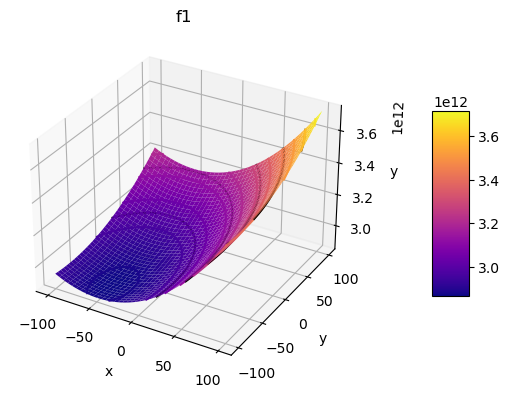
\includegraphics[width=\linewidth]{figuras/funciones_cec2017/shifted_rotated_f1.png}
        \caption{\(f_1\): función unimodal \textit{Bent Cigar}.}
    \end{subfigure}
    \hfill
    \begin{subfigure}[t]{0.45\textwidth}
        \centering
        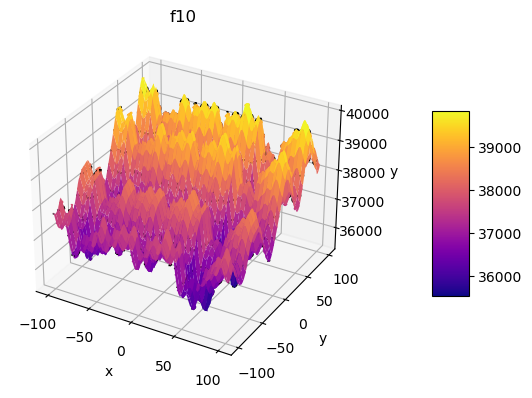
\includegraphics[width=\linewidth]{figuras/funciones_cec2017/f10.png}
        \caption{\(f_{10}\): función multimodal \textit{Schwefel}.}
    \end{subfigure}
    \caption{Representación ilustrativa de dos paisajes de
        búsqueda pertenecientes a la suite CEC2017.}
    \label{fig:paisajes_cec2017}
\end{figure}

La suite fue definida inicialmente con \textbf{30 funciones}, aunque revisiones posteriores eliminaron \(f_2\) debido a su inestabilidad numérica. En este trabajo, consideramos la suite completa ya que es la expuesta por la implementación empleada.

\begin{table}[H]
    \centering
    \begin{tabular}{lc}
        \toprule
        \textbf{Familia}     & \textbf{Funciones}     \\
        \midrule
        Unimodales           & \(f_1\)--\(f_3\)       \\
        Multimodales simples & \(f_4\)--\(f_{10}\)    \\
        Híbridas             & \(f_{11}\)--\(f_{20}\) \\
        Compuestas           & \(f_{21}\)--\(f_{30}\) \\
        \bottomrule
    \end{tabular}
    \caption{Familias de funciones de CEC2017 según la numeración empleada en este trabajo.}
    \label{tab:familias_cec2017}
\end{table}

Los detalles concretos de la integración software del benchmark y de la
interfaz de evaluación empleada se recogen en la
Sección~\ref{sec:detalles_implementacion}.

% \subsection{Funciones consideradas en cada fase experimental}

% % Distingue entre la suite completa y el subconjunto representativo utilizado para el cribado y el ajuste fino.

% El uso de CEC2017 se adapta a los objetivos y al coste computacional de cada
% fase experimental. Para analizar el comportamiento de las metaheurísticas y
% evaluar las distintas configuraciones del mecanismo de reinicio elitista se
% utilizan las \textbf{30 funciones} expuestas por la implementación empleada. Esta evaluación permite comprobar la robustez de cada configuración sobre paisajes de búsqueda diversos antes de generar las trayectorias destinadas al estudio de los modelos subrogados.

% Dado el elevado coste computacional que supondría ejecutar múltiples combinaciones de modelos, estrategias de entrenamiento y semillas sobre el benchmark completo, esta fase se realiza sobre un subconjunto fijo de \textbf{siete funciones} seleccionadas para cubrir las cuatro familias descritas anteriormente:

% 
\begin{table}[H]
    \centering
    \begin{adjustbox}{max width=0.55\textwidth}
        \begin{tabular}{lc}
            \toprule
            \textbf{Familia} & \textbf{Funciones} \\
            \midrule
            Unimodales       & \(f_1\)            \\
            Multimodales     & \(f_4, f_{10}\)    \\
            Híbridas         & \(f_{12}, f_{18}\) \\
            Compuestas       & \(f_{22}, f_{29}\) \\
            \bottomrule
        \end{tabular}
    \end{adjustbox}
    \caption{Funciones seleccionadas para la evaluación inicial de las técnicas subrogadas.}
    \label{tab:funciones_cribado_surrogate}
\end{table}

% Este subconjunto permite identificar los modelos y las estrategias de
% entrenamiento más prometedores antes de abordar las fases posteriores del
% estudio, reservando la validación sobre el benchmark
% completo para las configuraciones finales que superen con éxito esta fase de
% cribado.

%%%%%%%%%%%%%%%%%%%%%%
\section{Estrategias de resolución: Metaheurísticas}
\label{sec:metaheuristicas}

% Expone las condiciones bajo las que AGE, DE y SHADE generan las trayectorias.


% Indica dimensión, dominio, presupuesto de evaluaciones, tamaño de población y semillas.

% Recoge en tablas los parámetros específicos de cada algoritmo.

Las metaheurísticas AGE, DE y SHADE, descritas en el
Capítulo~\ref{chap:algo_tecnicas_ref}, se ejecutan bajo las mismas condiciones
con el objetivo de obtener historiales de evaluaciones comparables. Todas las pruebas
se realizan en dimensión \(D=10\), sobre el dominio de búsqueda
\([-100,100]^{10}\), y utilizan un tamaño de población fijo de \textbf{50 individuos.}

El criterio de parada se establece mediante el número de evaluaciones de la
función objetivo. Siguiendo la definición propia de CEC2017, cada ejecución
dispone de un presupuesto máximo de \(10000 \cdot D\) evaluaciones. Por tanto,
al considerar \(D=10\), el límite se fija en \(100000\) evaluaciones por
ejecución.

Dado que las metaheurísticas consideradas incorporan \textbf{componentes aleatorias}, una única ejecución no resulta suficiente para valorar su comportamiento. Por este motivo, cada combinación de función y metaheurística se ejecuta un total de \textbf{\(51\) veces}.

\begin{table}[H]
    \centering
    \begin{adjustbox}{max width=\textwidth}
        \begin{tabular}{lc}
        \toprule
        \textbf{Parámetro}                   & \textbf{Valor}            \\
        \midrule
        Dimensión del problema               & \(D=10\)                  \\
        Dominio de búsqueda                  & \([-100,100]^{10}\)       \\
        Presupuesto máximo de evaluaciones   & \(100000\)                \\
        Tamaño de la población               & \(50\)                    \\
        Número de ejecuciones independientes & \(51\)                    \\
        \bottomrule
        \end{tabular}
    \end{adjustbox}
    \caption{Parámetros comunes utilizados en la ejecución de las
        metaheurísticas.}
    \label{tab:parametros_comunes_metaheuristicas}
\end{table}


A partir del entorno de evaluación definido, cada metaheurística mantiene la
configuración propia de su esquema de búsqueda. Los operadores y particularidades de los
algoritmos se desarrollaron en el Capítulo~\ref{chap:algo_tecnicas_ref}, por lo
que a continuación se recogen únicamente los valores utilizados durante la
generación del histórico de evaluaciones.

\begin{enumerate}
    \item \textbf{AGE:} para la implementación propia se utilizan los parámetros recogidos en la Tabla~\ref{tab:parametros_age}.

          \begin{table}[htbp]
              \centering
              \begin{adjustbox}{max width=\textwidth}
                  \begin{tabular}{lc|lc}
                      \toprule
                      \textbf{Parámetro}                              & \textbf{Valor} &
                      \textbf{Parámetro}                              & \textbf{Valor}   \\
                      \midrule
                      \textbf{Tamaño del torneo}                      & \(2\)          &
                      \textbf{Probabilidad de cruce}                  & \(0.7\)          \\
                      \textbf{Probabilidad de mutación}               & \(0.1\)        &
                      \textbf{Parámetro \(\alpha\) de BLX-\(\alpha\)} & \(0.45\)         \\
                      \textbf{Desviación típica de la mutación}       & \(0.3\)        &
                                                                      &                  \\
                      \bottomrule
                  \end{tabular}
              \end{adjustbox}
              \caption{Parámetros utilizados para AGE.}
              \label{tab:parametros_age}
          \end{table}

    \item \textbf{DE:} se emplea la variante DE/rand/1/bin por defecto de la implementación empleada (véase en la
          Tabla~\ref{tab:parametros_de}).

          \begin{table}[htbp]
              \centering
              \begin{adjustbox}{max width=\textwidth}
                  \begin{tabular}{lc|lc}
                      \toprule
                      \textbf{Parámetro}                    & \textbf{Valor} &
                      \textbf{Parámetro}                    & \textbf{Valor}   \\
                      \midrule
                      \textbf{Estrategia de mutación}       & DE/rand/1      &
                      \textbf{Operador de cruce}            & Binomial         \\
                      \textbf{Factor de escala \(F\)}       & \(0.5\)        &
                      \textbf{Probabilidad de cruce \(CR\)} & \(0.9\)          \\
                      \bottomrule
                  \end{tabular}
              \end{adjustbox}
              \caption{Parámetros utilizados para DE.}
              \label{tab:parametros_de}
          \end{table}

    \item \textbf{SHADE:} se mantiene la configuración por defecto de la implementación empleada (véase en
          la Tabla~\ref{tab:parametros_shade}).

          \begin{table}[htbp]
              \centering
              \begin{adjustbox}{max width=\textwidth}
                  \begin{tabular}{lc|lc}
                      \toprule
                      \textbf{Parámetro}                    & \textbf{Valor}     &
                      \textbf{Parámetro}                    & \textbf{Valor}       \\
                      \midrule
                      \textbf{Estrategia de mutación}       & current-to-pbest/1 &
                      \textbf{Operador de cruce}            & Binomial             \\
                      \textbf{Factor de escala \(F\)}       & Adaptativo         &
                      \textbf{Probabilidad de cruce \(CR\)} & Adaptativa           \\
                      \textbf{Tam. de la mem. histórica}    & \(100\)            &
                                                            &                      \\
                      \bottomrule
                  \end{tabular}
              \end{adjustbox}
              \caption{Parámetros utilizados para SHADE.}
              \label{tab:parametros_shade}
          \end{table}

\end{enumerate}


\subsection{Criterio de reinicio elitista}
\label{subsec:criterio_reinicio}

Para identificar situaciones de \textbf{estancamiento}, se utilizan gráficas de convergencia y diversidad. Si se detecta este comportamiento, se incorpora el mecanimos de reinicio descrito en el Capítulo~\ref{chap:algo_tecnicas_ref}, parametrizado medienta una ventana de estancamiento $\rho$ que expresa, como \textbf{proporción del presupuesto total de evaluaciones}, el tiempo sin mejoras a partir del cual se considera que el algoritmo ha convergido prematuramente.

Tal y como está definido, es necesario definir el criterio de activación, y por tanto, determinar cuándo una variación del segundo mejor individuo se corresponde con una mejora efectiva. Dado que CEC2017 considera nulos los valores por debajo de $10^{-8}$, cualquier variación de \textit{fitness} de menor orden corresponde a ruido numérico. Para descartarlas sin filtrar progresos reales, se contabilizan como mejora únicamente aquellas variaciones cuya magnitud supere una \textbf{tolerancia} de $10^{-6}$.

El impacto de este mecanismo sobre la búsqueda se evalúa con un conjunto de configuraciones del criterio frente a la versión \textit{base} sin reinicio, correspondiente a valores de $\rho$ del $1\%$, $3\%$, $5\%$, $7\%$ y $10\%$.

El análisis se realiza de forma \textbf{independiente} por cada algoritmo ya que el objetivo no es comparar AGE, DE y SHADE entre sí, sino determinar qué configuración de cada uno resulta más adecuada para generar un históral de evaluaciones útil en la fase subrogada. Para ello, se utiliza el \textbf{ranking medio}, agregando los resultados sobre todas las funciones sin que las de mayor magnitud de error distorsionen la agregación.

%%%%%%%%%%%%%%%%%%%%%%
\section{Registro temporal de evaluaciones}
\label{sec:generacion_trayectorias}

Durante la ejecución de las metaheurísticas se registran cronológicamente las
evaluaciones reales realizadas sobre la función objetivo.

En lugar de analizar únicamente el resultado final de cada ejecución, este trabajo utiliza la secuencia temporal de soluciones evaluadas para estudiar cómo evoluciona la información disponible a lo largo de la búsqueda y cómo puede aprovecharse posteriormente en la fase de evaluación subrogada sobre el histórico de datos.

Para cada evaluación se registra el vector de decisión
\(\mathbf{x} \in \mathbb{R}^{D}\), el valor real de \textit{fitness} obtenido al
evaluar la función objetivo y un \textbf{identificador temporal} que indica el orden en el que se generó la muestra. La Tabla~\ref{tab:estructura_trayectorias}
resume la información registrada y su utilidad posterior.

\begin{table}[H]
    \centering
    \begin{tabular}{l p{9.4cm}}
        \toprule
        \textbf{Campo} & \textbf{Descripción}                                                                                            \\
        \midrule
        \texttt{eval\_id}
                       & Identificador que refleja el orden cronológico de evaluación para la posterior partición en bloques temporales. \\
        \midrule
        \(\mathbf{x}\)
                       & Vector de decisión asociado a la solución candidata.                                                            \\
        \midrule
        \textit{fitness}
                       & Valor real obtenido al evaluar la función objetivo.                                                             \\
        \bottomrule
    \end{tabular}
    \caption{Información registrada para cada evaluación.}
    \label{tab:estructura_trayectorias}
\end{table}

A partir de este histórico de evaluaciones, cada ejecución se organiza posteriormente en bloques temporales que permiten construir los conjuntos de entrenamiento y validación empleados en la evaluación posterior de los modelos subrogados.

%%%%%%%%%%%%%%%%%%%%%%
\section{Técnicas subrogadas: modelos candidatos y de referencia}

Los modelos empleados en este trabajo se presentaron conceptualmente en el Capítulo~\ref{chap:algo_tecnicas_ref}. Esta sección se centra en cómo se preparan los datos antes de entrenar cada modelo y qué configuración concreta se utiliza en la Sección~\ref{subsec:comparacion_modelos}.

\subsection{Configuración experimental de los modelos}

Como se comentó en la Sección \ref{sec:tecnicas_subrogadas}, Kriging y
PCE se incorporan como técnicas clásicas de referencia, por lo que no forman
parte del mismo protocolo experimental aplicado inicialmente al resto de
regresores.

Para garantizar una comparación no sobreajustada a los problemas de optimización de CEC2017, metaheurística o semilla, se mantienen algunos parámetros en sus valores por defecto y se modifican los que sí merecen ser ajustados para evitar comportamientos sesgados. La configuración no predeterminada empleada en cada modelo se recoge en la Tabla~\ref{tab:surrogate_models_config}.

%% hay que cambiar la implementacion de pce

\begin{table}[htbp]
    \centering
    \begin{tabular}{l p{7cm}}
        \toprule
        \textbf{Modelo} & \textbf{Configuración no predeterminada}                                                \\
        \midrule
        LASSO           & \makecell[l]{\texttt{alpha=0.01}                                                        \\ \texttt{max\_iter=5000} \\ \texttt{random\_state=42}} \\
        \midrule
        RSM             & \texttt{PolynomialFeatures} sobre regresión lineal ordinaria. Configuración por defecto \\
        \midrule
        RBF             & \makecell[l]{\texttt{neighbors=50}                                                      \\ \texttt{smoothing=1} \\ \texttt{kernel=gaussian} \\ \texttt{degree=-1} \\ \texttt{epsilon=1.0}} \\
        \midrule
        SVR             & Configuración por defecto                                                               \\
        \midrule
        MLP             & \makecell[l]{\texttt{hidden\_layer\_sizes=(128,\,64)}                                   \\ \texttt{alpha=1e-3} \\ \texttt{max\_iter=2000} \\ \texttt{random\_state=42} \\ \texttt{early\_stopping=True}} \\
        \midrule
        Random Forest   & \makecell[l]{\texttt{n\_estimators=200}                                                 \\ \texttt{max\_depth=16} \\ \texttt{min\_samples\_leaf=5} \\ \texttt{max\_features=0.5} \\ \texttt{random\_state=42} \\ \texttt{n\_jobs=-1}} \\
        \midrule
        HGB             & \makecell[l]{\texttt{max\_iter=200}                                                     \\ \texttt{learning\_rate=0.05} \\ \texttt{max\_depth=4} \\ \texttt{l2\_regularization=1e-3} \\ \texttt{random\_state=42}} \\
        \midrule
        XGBoost         & \makecell[l]{\texttt{n\_estimators=400}                                                 \\ \texttt{max\_depth=4} \\ \texttt{learning\_rate=0.05} \\ \texttt{subsample=0.8} \\ \texttt{colsample\_bytree=0.8} \\ \texttt{random\_state=42} \\ \texttt{n\_jobs=-1} \\ \texttt{tree\_method=hist}} \\
        \midrule
        Kriging         & \texttt{corr=matern52}                                                                  \\
        \midrule
        PCE             & \texttt{order=3}                                                                        \\
        \bottomrule
    \end{tabular}
    \caption{Configuración inicial empleada para la evaluación de los modelos subrogados.}
    \label{tab:surrogate_models_config}
\end{table}

\subsection{Preprocesamiento de los datos}
\label{subsec:preprocesamiento}

Antes de entrenar cada modelo, los datos generados por las distintas metaheurísticas requieren dos \textbf{transformaciones independientes} que afectan, respectivamente, a las variables de entrada y a la variable objetivo.

\textbf{Escalado de las variables de entrada.} Para mantener un protocolo homogéneo y robusto entre modelos, \textbf{todas las técnicas} se entrenan con las variables de entrada escaladas. Esta transformación es especialmente importante en técnicas sensibles a la magnitud de las variables, como LASSO, MLP, SVR, RBF y RSM. Aunque no es estrictamente necesario para el resto, se mantiene también en estos casos para mantener la consistencia del procedimiento experimental. Dado que en \textbf{CEC2017} las variables de decisión se definen sobre el dominio \([-100,100]^{D}\), todas las muestras se reescalan al intervalo \([-1,1]^{D}\) mediante la transformación \[
    x_{j}^{\ast} = \frac{x_{j}}{100}.
\]
De este modo, se evitan diferencias de escala innecesarias entre variables y se aplica el mismo preprocesamiento a todos los modelos considerados.

\textbf{Escalado de la variable objetivo.} En algunos modelos, la escala de la variable objetivo puede influir directamente en el ajuste. Por este motivo, se estandiraza el valor de \textit{fitness} únicamente en aquellos modelos donde resulta necesario: LASSO, RSM, RBF, SVR y MLP. En estos casos, y a partir de las formulaciones matemáticas de cada modelo definidas en el Capítulo~\ref{chap:algo_tecnicas_ref}, la magnitud de \(y\) puede afectar a la regularización, al condicionamiento numérico o al proceso de optimización interno del modelo.

Para los modelos en los que sí se estandariza la variable objetivo, se utiliza la transformación
\[
    y^{\ast} = \frac{y - \mu_{y}}{\sigma_{y}}, \qquad
    \mu_{y} = \frac{1}{n}\sum_{i=1}^{n} y_{i}, \qquad
    \sigma_{y} = \sqrt{\frac{1}{n}\sum_{i=1}^{n} (y_{i} - \mu_{y})^{2}}.
\]
Los valores $\mu_{y}$ y $\sigma_{y}$ se calculan \textbf{exclusivamente sobre el conjunto de entrenamiento}, evitando así filtraciones de información (\textit{data leakage}) desde el conjunto de validación. Tras la predicción, el resultado se devuelve a la escala original del problema mediante la \textbf{transformación inversa}, de forma que todos los modelos se comparan sobre los valores reales de  \textit{fitness}.

\section{Métricas empleadas}

Para evaluar el rendimiento de los modelos subrogados se utilizan distintas métricas que podemos agrupar en tres familias complementarias: el \textbf{error de predicción}, la \textbf{capacidad de ordenación} y el \textbf{coste computacional}.

\subsection{Error de predicción}

La capacidad de predicción de un modelo determina su calidad como regresor.
Para cuantificarla se emplean el \textbf{error absoluto medio} (MAE) y la
\textbf{raíz del error cuadrático medio} (RMSE), junto con sus correspondientes
versiones normalizadas.

Dado un conjunto de validación formado por \(n\) pares
\(\{(\mathbf{x}_i, y_i)\}_{i=1}^{n}\), donde \(y_i\) es el valor real del
\textit{fitness} y \(\hat{f}(\mathbf{x}_i)\) la predicción del modelo, ambas
métricas se definen como


\begin{equation}
    \text{MAE} = \frac{1}{n}\sum_{i=1}^{n} \bigl|y_i - \hat{f}(\mathbf{x}_i)\bigr|,
    \label{eq:mae}
\end{equation}

\begin{equation}
    \text{RMSE} = \sqrt{\frac{1}{n}\sum_{i=1}^{n} \bigl(y_i - \hat{f}(\mathbf{x}_i)\bigr)^2}.
    \label{eq:rmse}
\end{equation}

La diferencia entre ambas es la \textbf{sensibilidad al penalizar errores de mayor magnitud}. A diferencia del MAE, el RMSE penaliza con mayor intensidad \textbf{casos atípicos}, por lo que resulta muy útil para detectar fallos puntuales relevantes.

Dado que las funciones de CEC2017 presentan rangos de \textit{fitness} muy distintos, los valores absolutos de MAE y RMSE no resultan comparables entre funciones ni entre bloques temporales de una mismo histórico de evaluaciones. Para facilitar su interpretación, ambas se normalizan dividiéndolas por la media de los valores absolutos del \textit{fitness} real en el conjunto de validación, denotada como \(\bar{|y|} = \frac{1}{n}\sum_{i=1}^{n}|y_i|\):

\begin{equation}
    \text{NMAE} = \frac{\text{MAE}}{\bar{|y|}},
    \label{eq:nmae}
\end{equation}

\begin{equation}
    \text{NRMSE} = \frac{\text{RMSE}}{\bar{|y|}}.
    \label{eq:nrmse}
\end{equation}

En este caso, los valores próximos a cero indican que las predicciones se
mantienen cercanas a los valores reales de \textit{fitness}.

\subsection{Capacidad de ordenación}

Como se expuso en la
Sección~\ref{subsec:clasificacion_surrogates_prediccion}, la utilidad de un
modelo subrogado dentro de una metaheurística no depende únicamente de su
precisión numérica. Un modelo subrogado puede realizar predicciones que no son precisas pero puede ser capaz de ordenar correctamente las soluciones candidatas.

Para evaluar esta propiedad se
emplea el \textbf{coeficiente de correlación de Spearman}, que cuantifica el grado de concordancia ordinal
entre los valores reales y los predichos.

El coeficiente se calcula como la correlación de Pearson aplicada a los rangos de ambas distribuciones. Sea \(R_i\) el rango del valor real del \textit{fitness} de la muestra \(i\) dentro del conjunto de validación, y \(Q_i\) el rango de la predicción correspondiente. Entonces:

\begin{equation}
    \rho_s
    =
    \frac{
        \displaystyle\sum_{i=1}^{n}
        (R_i - \bar{R})(Q_i - \bar{Q})
    }{
        \sqrt{
            \displaystyle\sum_{i=1}^{n}(R_i - \bar{R})^2
            \cdot
            \displaystyle\sum_{i=1}^{n}(Q_i - \bar{Q})^2
        }
    },
    \label{eq:spearman}
\end{equation}
donde \(\bar{R}\) y \(\bar{Q}\) son los rangos medios.

El coeficiente toma valores en \([-1, 1]\). Un valor \(1\) indica concordancia perfecta de orden, \(-1\) refleja un orden completamente invertido, y \(0\) señala ausencia de relación ordinal.

Cuando dos o más valores coinciden, se les asignan rangos consecutivos según
su orden de aparición en el vector correspondiente. De este modo, incluso si
un subrogado genera predicciones constantes, se mantiene una ordenación total
determinista y el coeficiente puede calcularse de forma consistente entre
ejecuciones.

% En la implementación, los rangos se obtienen mediante
% \texttt{scipy.stats.rankdata(\ldots, method="ordinal")} y posteriormente se
% calcula la correlación entre dichos rangos mediante \texttt{scipy.stats.pearsonr}.

\subsection{Coste computacional}

La viabilidad de un modelo subrogado para la hibridación también depende de su coste computacional:

\begin{itemize}
    \item \textbf{Tiempo de entrenamiento:} tiempo necesario, en segundos, para ajustar el modelo sobre el conjunto de entrenamiento.
    \item \textbf{Tiempo de predicción:} tiempo requerido, en segundos, para evaluar el modelo sobre las muestras del conjunto de validación.
\end{itemize}

Un modelo con un tiempo de entrenamiento elevado puede no ser adecuado si debe reajustarse varias veces durante la ejecución. Del mismo modo, un tiempo de predicción alto reduce la ventaja de usar el subrogado para filtrar candidatos antes de realizar evaluaciones reales. Por tanto, ambos deben analizarse conjuntamente para identificar configuraciones cuyo coste pueda comprometer su posterior integración.

\subsection{Criterio de comparación de los modelos}
\label{subsec:criterio_comparacion_modelos}

A lo largo de este trabajo, la comparación entre modelos se realiza analizando conjuntamente las métricas anteriores. Estas se presentan a continuación en orden de importancia:

\begin{enumerate}
    \item \textbf{Coeficiente de Spearman:} permite valorar si el subrogado preserva el orden relativo de calidad entre las soluciones candidatas.
    \item \textbf{Coste computacional:} analiza la viabilidad para la posterior hibridación.
          \begin{enumerate}
              \item \textbf{Tiempo de predicción}
              \item \textbf{Tiempo de entrenamiento}
          \end{enumerate}
    \item \textbf{NMAE y NRMSE:} se emplean como métricas complementarias para evaluar la calidad predictiva ya que no es el objetivo de este trabajo.
\end{enumerate}

%%%%%%%%%%%%%%%%%%%%%%
\section{Evaluación de modelos subrogados sobre históricos de evaluaciones}

Los datos de búsqueda generados por las metaheurísticas se organizan en \textbf{cinco bloques temporales consecutivos}, cada uno de ellos correspondiente al \textbf{20\,\% del presupuesto total de evaluaciones}. Dado que cada ejecución comprende \(100\,000\) evaluaciones, cada bloque agrupa \(20\,000\) muestras, ordenadas cronológicamente según el instante en que fueron generadas durante la búsqueda. Los bloques se identifican por el intervalo porcentual que ocupan dentro de las evaluaciones realizadas: \textbf{1--20\,\%}, \textbf{21--40\,\%}, \textbf{41--60\,\%}, \textbf{61--80\,\%} y \textbf{81--100\,\%}.

A partir de esta partición, las dos estrategias definidas en la
Sección~\ref{sec:metodologia_estrategias_offline} se instancian en este trabajo mediante los
conjuntos de entrenamiento recogidos en la
Tabla~\ref{tab:pares_entrenamiento_validacion}. La \textbf{estrategia no acumulativa} utiliza un único bloque en cada ajuste, mientras que la \textbf{acumulativa} incorpora progresivamente todos los bloques disponibles hasta el instante considerado.

\begin{table}[H]
    \centering
    \renewcommand{\arraystretch}{1.15}
    \begin{adjustbox}{max width=\textwidth}
        \begin{tabular}{c|c c|c c|c}
            \toprule
            \multirow{2}{*}{\textbf{Bloque}} & \multicolumn{2}{c|}{\textbf{No acumulativa}} & \multicolumn{2}{c|}{\textbf{Acumulativa}}                                                & \multirow{2}{*}{\makecell{\textbf{Bloque}                                  \\\textbf{de validación}}} \\
            \cmidrule(lr){2-3} \cmidrule(lr){4-5}
                                             & Intervalo                                    & \makecell{\textbf{Tamaño}                                                                                                                                             \\ \textbf{entrenamiento}} & Intervalo & \makecell{\textbf{Tamaño} \\ \textbf{entrenamiento}} & \\
            \midrule
            $B_1$                            & 1--20\,\%                                    & 20\,000                                                                                  & 1--20\,\%                                 & 20\,000 & $B_2$\ (21--40\,\%)  \\
            $B_2$                            & 21--40\,\%                                   & 20\,000                                                                                  & 1--40\,\%                                 & 40\,000 & $B_3$\ (41--60\,\%)  \\
            $B_3$                            & 41--60\,\%                                   & 20\,000                                                                                  & 1--60\,\%                                 & 60\,000 & $B_4$\ (61--80\,\%)  \\
            $B_4$                            & 61--80\,\%                                   & 20\,000                                                                                  & 1--80\,\%                                 & 80\,000 & $B_5$\ (81--100\,\%) \\
            $B_5$                            & 81--100\,\%                                  & \multicolumn{4}{c}{\cellcolor{gray!10}\textbf{Reservado exclusivamente para validación}}                                                                              \\
            \bottomrule
        \end{tabular}
    \end{adjustbox}
    \caption{Resumen de las particiones utilizadas para construir los conjuntos de entrenamiento y validación en ambas estrategias.}
    \label{tab:pares_entrenamiento_validacion}
\end{table}

Como se observa en la tabla, el bloque~5 queda reservado exclusivamente para validación al no haber más muestras sobre las que validar el modelo si utilizase dicho bloque como entrenamiento.

Para que los resultados sean comparables y no dependan del tamaño del conjunto de entrenamiento empleado, el conjunto de validación se toma siempre del bloque temporal inmediatamente posterior al último bloque utilizado para entrenar el mdoelo. Como cada bloque contiene \(20000\)
evaluaciones, se selecciona el \textbf{25\% de sus muestras}, es decir, \textbf{5000 soluciones} evaluadas por ejecución. Este criterio se aplica tanto en la estrategia acumulativa como en la no acumulativa, de forma que el tamaño del conjunto de validación no depende del número de bloques empleadas en el entrenamiento.

La selección de las muestras se realiza de forma determinista a partir de la semilla de la ejecución y del bloque temporal utilizado para validación. De esta forma, para una misma ejecución y un mismo bloque, el conjunto de validación queda fijado y es común a todos los modelos y estrategias evaluados.

Dado el coste computacional de evaluar todas las combinaciones de modelos, estrategias de entrenamiento y semillas sobre la suite completa, la primera comparación se realiza sobre un subconjunto de funciones de CEC2017. En esta fase se mantienen las \(51\) semillas empleadas en las ejecuciones de las metaheurísticas, pero se reduce el número de funciones para hacer viable la comparación inicial entre modelos.

El subconjunto se elige para cubrir las principales familias de funciones del benchmark:

\begin{itemize}
    \item \textbf{Unimodal:} \(f_1\).
    \item \textbf{Multimodal:} \(f_4\), \(f_{10}\).
    \item \textbf{Híbrida:} \(f_{12}\), \(f_{18}\).
    \item \textbf{Compuesta:} \(f_{22}\), \(f_{29}\).
\end{itemize}

Con esta selección se comparan los modelos en funciones con características distintas, sin elevar innecesariamente el coste experimental. Las configuraciones seleccionadas en esta fase se evalúan posteriormente sobre la suite completa.

%%%%%%%%%%%%%%%%%%%%%%
\section{Ajuste fino de hiperparámetros}
\label{sec:protocolo_ajuste_hiperparametros}

%% objetivo del ajuste fino: Explicar que no se busca rediseñar todos los modelos, sino refinar los hiperparámetros de los modelos candidatos tras el cribado offline

% idea clave: El ajuste fino no constituye una nueva fase de comparación global entre todos los regresores, sino una optimización acotada de los modelos que hayan mostrado mejor comportamiento en la fase offline.

El ajuste fino de hiperparámetros se plantea como una fase posterior a la decisión de la mejor estrategia y la comparación inicial de modelos. Su objetivo no es repetir la comparación completa entre todos los regresores, sino refinar la configuración de aquellos que hayan obtenido mejores resultados antes de evaluarlos sobre la suite completa. De esta forma, el coste experimental se concentra en el modelo o modelos con mayor probabilidad de resultar útiles en una posterior integración.

Dado que el coste de entrenamiento y predicción no es el mismo para todos los modelos, el número de semillas usado en esta fase puede variar según la técnica considerada. Cuando dicho coste sea elevado, el ajuste se realizará sobre un subconjunto fijo de semillas para que la búsqueda de hiperparámetros sea asumible.
Esta reducción afecta únicamente a la fase de ajuste, ya que la configuración o configuraciones finalmente seleccionadas se comparan posteriormente sobre las \(30\) funciones de CEC2017
y las \(51\) semillas empleadas para el histórico de evaluaciones.

El procedimiento mantiene el orden temporal de los datos generados por cada metaheurística. Para evitar que la elección de hiperparámetros utilice información posterior al bloque de entrenamiento (\textit{data leakage}), se aplica una partición interna dentro de dicho bloque:

\begin{itemize}
    \item El \textbf{80\% inicial} de las muestras del bloque se utiliza para el entrenamiento de las distintas configuraciones candidatas que componen el espacio de búsqueda.
    \item El \textbf{20\% final} de dicho bloque se reserva como conjunto de validación interna para evaluar el rendimiento de cada configuración y estimar su capacidad de generalización dentro de la misma etapa temporal.
\end{itemize}

Una vez elegida la configuración, el modelo se reentrena con todas las muestras del bloque de entrenamiento y se evalúa sobre un subconjunto del bloque temporal inmediatamente posterior (conjunto de validación). Así, las muestras futuras no intervienen en la selección de hiperparámetros, sino solo en la evaluación del modelo ya ajustado.

La Figura~\ref{fig:ajuste_hiperparametros_validacion_interna} representa este
procedimiento para una transición concreta. En el ejemplo, el ajuste interno
se realiza sobre el bloque correspondiente al intervalo 20--40\% de la
búsqueda y la evaluación posterior utiliza muestras pertenecientes al
intervalo 40--60\%.


\begin{figure}[H]
    \centering
    \begin{tikzpicture}[
            scale=0.9,
            every node/.style={transform shape},
            bloque/.style={draw, minimum height=0.9cm, font=\footnotesize, align=center, inner sep=3pt},
            flecha/.style={->, thick}
        ]

        % Nodo de entrenamiento (superior)
        \node[bloque, minimum width=2.2cm, fill=blue!10] (train) at (0,0)
        {80\%\\Ajuste};
        % Nodo de validación interna, justo debajo
        \node[bloque, minimum width=1.3cm, fill=orange!15, below=1.0cm of train] (valint)
        {20\%\\Val.};

        % Etiqueta de etapa temporal arriba, centrada respecto ambos nodos
        \node[font=\footnotesize, above=0.42cm of train]
        {\textbf{Entrenamiento 20--40\%}};

        % Selección de hiperparámetros a la derecha, alineada verticalmente con train
        \node[bloque, minimum width=1.7cm, fill=gray!10, right=2.0cm of train] (select)
        {Selec.\\Hiperparam.};
        % Futuro a la derecha del anterior
        \node[bloque, minimum width=1.7cm, fill=green!12, right=1.7cm of select] (future)
        {Futuro\\40--60\%};

        % Flechas de proceso
        \draw[flecha] (train.east) -- (select.west);
        \draw[flecha] (valint.east) -- ([yshift=0.0cm]select.south west);

        % Unión de validación interna hacia la selección de hiperparámetros (desde la derecha de valint hacia abajo del bloque de selección)
        % Flecha de proceso hacia el futuro
        \draw[flecha] (select.east) -- (future.west);

    \end{tikzpicture}
    \caption[Esquema de validación interna para el ajuste de hiperparámetros]{Esquema de validación interna para el ajuste de hiperparámetros con los conjuntos de ajuste y validación dispuestos en paralelo.}
    \label{fig:ajuste_hiperparametros_validacion_interna}
\end{figure}

% Ajustes recomendados: scale ~0.80, fuente \footnotesize, minimum width y height menores, distancias proporcionadas.

La búsqueda de hiperparámetros se realiza de forma exhaustiva sobre un espacio acotado de valores definido y la selección final sigue el criterio definido en la Subsección~\ref{subsec:criterio_comparacion_modelos}.

Las configuraciones consideradas para los modelos finalistas se presentan junto con
sus resultados en el capítulo siguiente.

\section{Integración del modelo subrogado durante la búsqueda}
\label{sec:integracion_subrogado_busqueda}

La integración del modelo subrogado durante la búsqueda se evalúa mediante el mecanismo de filtrado definido en la Sección~\ref{sec:estrategia_online_integracion_surrogate}. En esta fase, a diferencia de la evaluación sobre históricos de evaluaciones, las predicciones del subrogado pueden modificar las decisiones de la metaheurística. Por tanto, la comparación ya no se limita a medir la calidad de ordenación del modelo, sino que trata la hibridación como una variante del algoritmo original.

Para mantener acotado el coste experimental, la integración no se aplica a todos los modelos candidatos. Solo se considera el modelo y la estrategia de entrenamiento seleccionados tras la evaluación previa y el ajuste de hiperparámetros. El objetivo es comprobar si el subrogado elegido mejora el comportamiento de la metaheurística cuando interviene directamente en el proceso de búsqueda, tomando como referencia la versión original sin subrogado.

A partir de este esquema, el protocolo de integración queda definido por las siguientes decisiones experimentales:

\begin{enumerate}
    \item \textbf{Periodo inicial de calentamiento.} El filtro subrogado no se activa desde el inicio, ya que primero es necesario disponer de evaluaciones reales para entrenar el primer modelo y que pueda generar predicciones útiles. Si \(E_{\max}\) es el presupuesto total y \(\alpha_{\text{warm}}\) la proporción reservada a esta fase, el número de evaluaciones iniciales es
          \[
              E_{\text{warm}} = \alpha_{\text{warm}} E_{\max}.
          \]
          En coherencia con la división temporal utilizada en la evaluación previa, este periodo inicial se fija en el \(20\%\) del presupuesto total de evaluaciones (\(\alpha_{\text{warm}}=0.20\)).

    \item \textbf{Conjunto de entrenamiento.} El modelo se entrena únicamente con evaluaciones reales ya
          observadas. La construcción de este conjunto mantiene el orden temporal
          de la búsqueda y queda determinada por la estrategia de entrenamiento
          seleccionada previamente.

    \item \textbf{Frecuencia de actualización.} Para evitar reentrenamientos
          excesivamente frecuentes que supongan un coste computacional excesivo o modelos desfasados, se estudian distintas
          frecuencias de actualización expresadas como proporción del conjunto
          temporal de entrenamiento. Los valores considerados son \(0.25\),
          \(0.50\) y \(0.75\).

    \item \textbf{Probabilidad de uso del filtro.} El subrogado no se consulta necesariamente para todos los candidatos generados. Para cada candidato se extrae \(u \sim \mathcal{U}(0,1)\), y el filtro se aplica solo si
          \[
              u < p_{\text{sub}},
          \]
          donde \(p_{\text{sub}}\) controla la proporción esperada de candidatos sometidos a preevaluación subrogada. Cuando esta condición no se cumple, el candidato sigue el flujo de evaluación real de la metaheurística original.

          Se consideran los valores \(p_{\text{sub}} \in \{0.25, 0.50,
          0.75\}\).

    \item \textbf{Tratamiento tras reinicio.} Después de un reinicio, la
          distribución de soluciones puede cambiar de forma brusca, reduciendo
          temporalmente la representatividad del modelo. Por ello, se evalúa un periodo de enfriamiento durante el cual el filtro permanece desactivado y solo se incorporan evaluaciones reales. Se
          consideran \(50\), \(100\) y \(500\) evaluaciones reales,
          equivalentes a \(1\), \(2\) y \(10\) poblaciones generadas para
          \(N=50\). No se escoge un mayor número de evaluaciones ya que podría ocurrir que el modelo se apagase durante gran parte del proceso de optimización.
\end{enumerate}

Al tratarse como variantes de las metaheurísticas originales, las ejecuciones híbridas mantienen las condiciones generales definidas en la Tabla~\ref{tab:parametros_comunes_metaheuristicas}.

No obstante, para la calibración de los parámetros de integración se emplea un subconjunto reducido de funciones y semillas, distinto al utilizado en las fases previas. Esta fase no busca una optimización exhaustiva, sino tratar de seleccionar una
configuración homogénea para las distintas
metaheurísticas. Por ello, las decisiones experimentales se evalúan sobre las funciones \(f_3\), \(f_5\), \(f_9\), \(f_{15}\), \(f_{19}\), \(f_{24}\) y \(f_{27}\), junto con \(10\) semillas independientes no utilizadas en la selección del modelo.

La comparación entre variantes sigue el criterio agregado definido en la
Sección~\ref{sec:metaheuristicas}, basado en rankings medios sobre CEC2017. Además, se consideran contadores propios de la integración, como el número de reentrenamientos, el tiempo dedicado al modelo y el porcentaje de candidatos rechazados por el filtro.

Una vez seleccionada la configuración, la evaluación final se realiza sobre las \(30\) funciones de CEC2017 y \(51\) semillas nuevas, distintas tanto de las usadas en la calibración como de las empleadas en la evaluación previa. En esta fase, la variante híbrida se compara con la metaheurística original sin intervención subrogada. También se incluyen como referencia las hibridaciones basadas en Kriging y PCE, descritas en la Sección~\ref{sec:tecnicas_subrogadas_clasicas}.

Los resultados de las distintas decisiones experimentales y las comparaciones descritas se presentan en el Capítulo~\ref{chap:experimentacion}.

% Si el subrogado se usa inmediatamente, puede estar entrenado sobre una distribución que ya no representa la nueva población.

% Por ello se introduce un periodo de enfriamiento o cooldown, durante el cual se priorizan evaluaciones reales antes de volver a confiar en el modelo.


% - indicar que la estrategia se evaluara con el modelo seleccionado en el capitulo 7 tras la fase offline y su correspondiente ajuste de hiperparametros


% La selección de la configuración online no se realiza únicamente a partir del menor error medio, sino atendiendo al compromiso entre rendimiento final, robustez entre metaheurísticas y funciones, y coste computacional añadido por el uso del subrogado. Dado que el objetivo es definir una estrategia homogénea de hibridación, se priorizan aquellas configuraciones que presentan buen comportamiento agregado y rankings estables, evitando decisiones condicionadas por una única función o metaheurística.


% Se selecciona una configuración homogénea priorizando el compromiso entre rendimiento final, robustez entre metaheurísticas y coste añadido. Aunque algunas configuraciones obtienen mejores resultados en casos concretos, la combinación cooldown=100, retrain_ratio=0.50 y p=0.50 ofrece el comportamiento agregado más equilibrado para AGE, DE y SHADE. Esta elección evita ajustar la hibridación de forma específica para cada algoritmo y permite evaluar la utilidad general del mecanismo online propuesto.


% La probabilidad de uso del filtro subrogado se ajusta mediante un piloto previo sobre un subconjunto representativo de funciones y semillas, manteniendo fijos el resto de parámetros de la integración. Este piloto no pretende realizar una optimización exhaustiva del hiperparámetro, sino seleccionar un valor robusto y homogéneo para las tres metaheurísticas antes de ejecutar la evaluación completa. Bajo este criterio, se prioriza el comportamiento agregado y el ranking medio frente a mejoras aisladas en una función o algoritmo concreto.

% Los parámetros de la integración online se fijan mediante pilotos previos sobre un subconjunto de funciones y semillas. Esta fase no busca una optimización exhaustiva de hiperparámetros, sino seleccionar una configuración homogénea y computacionalmente viable para las tres metaheurísticas. La evaluación definitiva de dicha configuración se realiza posteriormente sobre la suite completa, utilizando semillas distintas a las empleadas en los pilotos.

% Las semillas empleadas en los pilotos de calibración online se mantienen separadas tanto de las utilizadas en la generación de trayectorias y evaluación offline como de las utilizadas en la evaluación final de la configuración online seleccionada.

% No se incluyó el caso retrain_ratio=1.00, ya que el valor 0.75 ya representa una actualización poco frecuente del modelo y permitió evaluar el efecto de espaciar considerablemente los reentrenamientos. Dado que esta configuración mostró una degradación respecto a 0.50, se descartó ampliar el piloto hacia frecuencias aún menores de actualización, que previsiblemente incrementarían el riesgo de utilizar un modelo desfasado respecto a la región explorada.


% Para la calibración de la estrategia online se consideran tres parámetros específicos: el periodo de enfriamiento tras reinicio, la frecuencia de actualización del modelo y la probabilidad de uso del filtro. Los valores candidatos se recogen en la Tabla~X. Esta fase no pretende realizar una optimización exhaustiva de hiperparámetros, sino seleccionar una configuración homogénea y computacionalmente viable para AGE, DE y SHADE.

%%%%%%%%%%%%%%%%%%%%%%
\section{Detalles de la implementación}
\label{sec:detalles_implementacion}


A diferencia de las secciones anteriores, centradas en definir el protocolo experimental, esta sección recoge las principales decisiones técnicas tomadas para implementar y reproducir los experimentos.


\subsection{Bibliotecas y herramientas empleadas}

La implementación de este trabajo se ha desarrollado en \texttt{Python}, al tratarse de un lenguaje de programación ampliamente utilizado en computación científica, optimización numérica y aprendizaje automático. Gracias a la gran variedad de bibliotecas consolidadas en este ámbito, se homogeniza la integración de las metaheurísticas, modelos subrogados y herramientas de análisis, reduciendo la necesidad de implementar estas componentes desde cero y minimizando posibles errores en el desarrollo.


La integración del benchmark se realiza a partir del repositorio mantenido por Daniel Molina%
\footnote{\url{https://github.com/dmolina/cec2017real}}, basado en el código de referencia de la competición CEC2017 y escrito en \textit{C++}. Sobre este código se ha construido un adaptador común en \textit{Python}, de modo que AGE, DE y SHADE evalúen candidatos mediante una misma interfaz.

Las implementaciones de las metaheurísticas no proceden de una única biblioteca. AGE se ha desarrollado directamente en \textit{Python} a partir del pseudocódigo descrito en el Capítulo~\ref{chap:algo_tecnicas_ref}. En cambio, DE y SHADE parten de las implementaciones de \texttt{PyADE}%
\footnote{\url{https://github.com/xKuZz/pyade}}, que se han adaptado para utilizar la misma infraestructura común que AGE: interfaz de evaluación, registro de históricos e integración del mecanismo de reinicio. De esta forma se aprovechan implementaciones existentes de algoritmos, reduciendo el esfuerzo de desarrollo y manteniendo al mismo tiempo un protocolo homogéneo para las tres metaheurísticas consideradas.

En el caso de los modelos subrogados, la mayoría de los regresores se implementan mediante \textit{scikit-learn}, biblioteca de aprendizaje automático que proporciona una interfaz común para entrenamiento, predicción y ajuste de hiperparámetros. Además, el escalado de la variable objetivo descrito en la Sección~\ref{subsec:preprocesamiento} se realiza mediante \texttt{StandardScaler}, propio de esa misma librería. El modelo RBF se construye con \texttt{RBFInterpolator} de \textit{SciPy}, al ajustarse directamente a la formulación empleada en este trabajo. XGBoost utiliza su biblioteca oficial, ya que las consideradas no cuentan con implementación propia. Por último, Kriging y PCE se implementan mediante \textit{Surrogate Modeling Toolbox} (SMT), una biblioteca especializada en modelado subrogado que permite incorporar estas técnicas clásicas de referencia.

Para describir el comportamiento de estos modelos, las métricas de evaluación se calculan combinando funciones de \textit{scikit-learn}, \textit{SciPy} y \textit{NumPy}. En particular, \textit{scikit-learn} se utiliza para las métricas de error, mientras que \textit{SciPy} y \textit{NumPy} se emplean para las operaciones necesarias en las métricas normalizadas y en el cálculo de la correlación de Spearman.

El procesamiento posterior de los resultados obtenidos por los distintos experimentos combina varias herramientas:

\begin{itemize}
    \item Los ficheros \textbf{HDF5} se gestionan mediante \texttt{PyTables}.
    \item \texttt{pandas} se utiliza
          para agrupar ejecuciones, calcular medias y preparar las tablas del Capítulo~\ref{chap:experimentacion}.
    \item \texttt{Matplotlib} se emplea para generar el soporte visual de los resultados como las curvas de convergencia o de diversidad.
    \item \texttt{DEAP} se usa para el registro de estadísticas
          generacionales, mediante sus utilidades \texttt{Statistics} y \texttt{Logbook}.
    \item La comparación agregada de medias y rankings medios sobre el benchmark se obtiene mediante \textbf{TACOLAB}\footnote{\url{https://tacolab.org/}}, una herramienta web
          orientada al análisis comparativo de algoritmos de optimización.
\end{itemize}

Las versiones concretas de las principales liberías empleadas en el entorno experimental para poder reproducir los experimentos son:

\begin{itemize}
    \item \texttt{Python} 3.14.5
    \item \texttt{NumPy} 2.4.3
    \item \texttt{Matplotlib} 3.10.8
    \item \texttt{SciPy} 1.17.1
    \item \texttt{scikit-learn} 1.8.0
    \item \texttt{SMT} 2.14.0
    \item \texttt{XGBoost} 3.2.0
    \item \texttt{pandas} 3.0.1
    \item \texttt{PyADE} 0.0.2
    \item \texttt{DEAP} 1.4.3
    \item \texttt{PyTables} 3.11.1
\end{itemize}

Adicionalmente, la integración del benchmark CEC2017 requiere compilar el código de referencia escrito en C++. Para ello se han utilizado \texttt{CMake}~4.0.1 y \texttt{Apple Clang}~17.0.0.

\subsection{Registro y almacenamiento de resultados}

Los resultados generados por las metaheurísticas se almacenan de forma independiente para cada combinación de función, algoritmo y semilla en formato \textbf{HDF5 comprimido}, ya que permite manejar eficientemente grandes volúmenes de datos, con un tamaño reducido por la compresión sin perdida y manteniendo separados los distintos experimentos. Además, al conservar los datos en formato numérico, se preserva la precisión asociada al tipo de dato utilizado. El contenido de este fichero se corresponde con el especificado en la Tabla~\ref{tab:estructura_trayectorias}.

Además del fichero principal, durante la ejecución se generan ficheros
\textbf{JSON} y \textbf{CSV} auxiliares con estadísticas descriptivas de la
población, medidas de diversidad y metadatos asociados al mecanismo de
reinicio. Estos archivos no se emplean como variables de entrada para los modelos subrogados, pero sí son útiles para analizar la dinámica de búsqueda y construir gráficas informativas.

El resto de experimentos también genera archivos auxiliares que recogen, para cada función, metaheurística, semilla, bloque y
modelo, las métricas principales, los hiperparámetros empleados y
los tiempos de entrenamiento y predicción. En la integración del modelo subrogado durante la búsqueda, se registra además información específica sobre su uso, como el número de reentrenamientos, el tiempo dedicado al modelo o la proporción de candidatos filtrados.

De este modo, los datos principales de cada ejecución se almacenan en formatos compactos y eficientes y se reservan formatos más ligeros y fáciles de interpretar para el análisis de resultados.

\subsection{Reproducibilidad de los experimentos}

El equipo utilizado para las ejecuciones se corresponde con un MacBook Air, equipado con el procesador Apple M4, que dispone de 10 núcleos distribuidos en 4 de rendimiento y 6 de eficiencia, junto con 16~GB de memoria RAM unificada y el sistema operativo macOS 26.3. Los experimentos se han lanzado de forma \textbf{secuencial}, sin paralelización entre ejecuciones, aunque algunos modelos como Random Forest y XGBoost hacen uso de paralelización interna mediante \texttt{n\_jobs=-1}. Los tiempos de entrenamiento y predicción presentados son directamente comparables dentro del entorno descrito, al haberse obtenido bajo las mismas condiciones de ejecución.

Los experimentos descritos en este capítulo se organizan mediante distintos
programas de ejecución. Cada uno de ellos corresponde a una fase concreta del
estudio y permite modificar los parámetros necesarios sin alterar la
implementación de los algoritmos.

\begin{enumerate}
    \item \textbf{\texttt{ejecutar\_metaheuristicas.py}}: implementa el diseño propuesto en las
          Secciones~\ref{sec:benchmark} y~\ref{sec:metaheuristicas}. Ejecuta las metaheurísticas
          sobre CEC2017 y registra los históricos de evaluaciones descritos en la
          Sección~\ref{sec:generacion_trayectorias}.
    \item \textbf{\texttt{ejecutar\_no\_acumulativo.py}} y \textbf{\texttt{ejecutar\_acumulativo.py}}:
          realizan la evaluación temporal de los modelos subrogados. Ambos comparten los mismos
          parámetros; la diferencia se encuentra en la forma de construir el conjunto de
          entrenamiento, tal y como se describió anteriormente.
    \item \textbf{\texttt{ajustar\_hiperparametros.py}}: lleva a cabo el ajuste fino de
          hiperparámetros conservando la estructura temporal
          e introduciendo una partición interna dentro de cada bloque de entrenamiento.
    \item \textbf{\texttt{ejecutar\_metaheuristicas\_online.py}}: ejecuta las metaheurísticas consideradas sobre CEC2017, incorporando el filtro subrogado y registrando tanto el rendimiento final como los contadores asociados a la hibridación.
\end{enumerate}

Los parámetros de cada programa se recogen en el Apéndice~\ref{ap:parametros_experimentos}.

\chapter{Experimentación y resultados}
\label{chap:experimentacion}

%% que resultados se obtienen

En este capítulo se presentan los resultados obtenidos a partir del procedimiento experimental descrito en el Capítulo~\ref{chap:metodologia_experimental}. El análisis se organiza de forma progresiva, comenzando por el comportamiento de las metaheurísticas consideradas y avanzando posteriormente hacia la evaluación de los modelos subrogados y su integración en el proceso de optimización.

En primer lugar, se analiza el comportamiento de AGE, DE y SHADE con el fin de identificar posibles fases de estancamiento y valorar el efecto del reinicio elitista sobre las trayectorias generadas. A continuación, se comparan las estrategias \textit{offline} de evaluación de modelos subrogados, se seleccionan las técnicas más prometedoras y se realiza su ajuste de hiperparámetros. Finalmente, se estudia la integración \textit{online} del modelo seleccionado dentro del bucle de optimización.


% ============================================================
\section{Estancamiento de las metaheurísticas y evaluación del reinicio elitista}
\label{sec:resultados_reinicio}
% ============================================================

En esta primera parte del análisis se estudia el comportamiento de AGE, DE y SHADE en ausencia de reinicio, con el objetivo de comprobar si sus trayectorias mantienen una dinámica suficientemente informativa durante todo el presupuesto de evaluaciones. Una vez identificado el problema de estancamiento, se evalúa el criterio de reinicio definido en el Capítulo~\ref{chap:algo_tecnicas_ref}.

Este análisis tiene un papel auxiliar dentro del trabajo: el objetivo principal no es optimizar el criterio de reinicio en sí mismo, sino evitar que las trayectorias utilizadas posteriormente para la evaluación de subrogados queden dominadas por fases largas de convergencia prematura. Por tanto, la finalidad no es comparar las metaheurísticas entre sí, sino determinar si cada una de ellas necesita un mecanismo de reactivación y qué ventana de estancamiento resulta aceptable para generar datos más útiles sin deteriorar de forma relevante la calidad final.


% ------------------------------------------------------------
\subsection{Motivación del reinicio}
\label{subsec:motivacion_reinicio}
% ------------------------------------------------------------


En ausencia de reinicio, la dinámica de cada metaheurística determina por completo la distribución de las muestras generadas. Cuando la búsqueda deja de producir mejoras relevantes antes de agotar dicho presupuesto, las evaluaciones posteriores tienden a concentrarse en torno a valores de \textit{fitness} muy similares, lo que reduce la variabilidad disponible para entrenar y validar modelos subrogados.

La Figura~\ref{fig:convergencia_sin_reinicio} muestra las curvas de convergencia promedio para tres funciones con características de paisaje diferentes. En \(f_1\), los algoritmos alcanzan rápidamente una zona estable; en \(f_{10}\), el comportamiento es más gradual, pero también aparecen tramos prolongados con poca mejora; finalmente, en \(f_{29}\), las curvas presentan una caída inicial casi instantánea seguida de una evolución prácticamente plana. Con estos ejemplos se verifica como gran parte relevante de la trayectoria generada por una metaheurística puede quedar dominada por fases de mejora muy reducida o incluso inexistentes.

La consecuencia directa de este estancamiento sobre la calidad de los datos generados se aprecia al analizar la distribución del error por bloques temporales. La Figura~\ref{fig:bloques_sin_reinicio} divide el presupuesto en cinco bloques del 20\% y muestra la distribución del error logarítmico en cada uno de ellos para una función representativa.

Como se observa en la figura, los primeros bloques presentan una distribución amplia que cubre distintas regiones del espacio de búsqueda. Sin embargo, a medida que aumenta el número de evaluaciones, las muestras se concentran progresivamente en un rango estrecho de valores. Desde la perspectiva del aprendizaje subrogado, estas muestras tardías son menos discriminativas, ya que el modelo recibe evaluaciones muy similares entre sí y dispone de menos información para distinguir soluciones de distinta calidad.

\begin{figure}[H]
    \centering
    \begin{subfigure}[t]{0.8\textwidth}
        \centering
        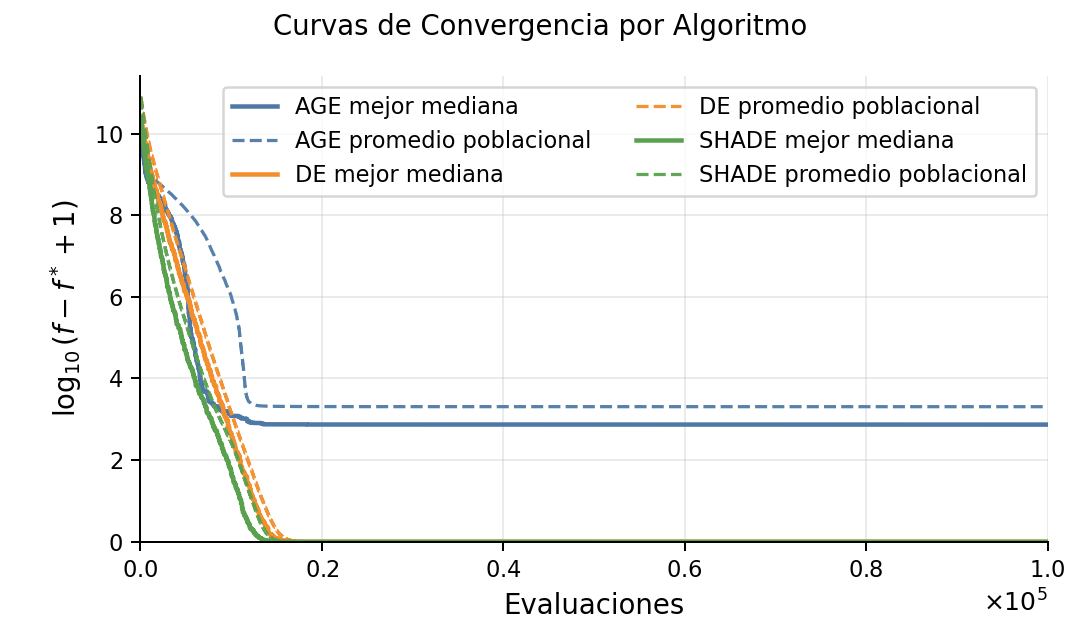
\includegraphics[width=\textwidth]{figuras/plots_sin_reinicio/curva_convergencia_cec2017_f1.png}
        \caption{\(f_1\)}
        \label{fig:convergencia_sin_reinicio_f1}
    \end{subfigure}
    \hfill
    \begin{subfigure}[t]{0.8\textwidth}
        \centering
        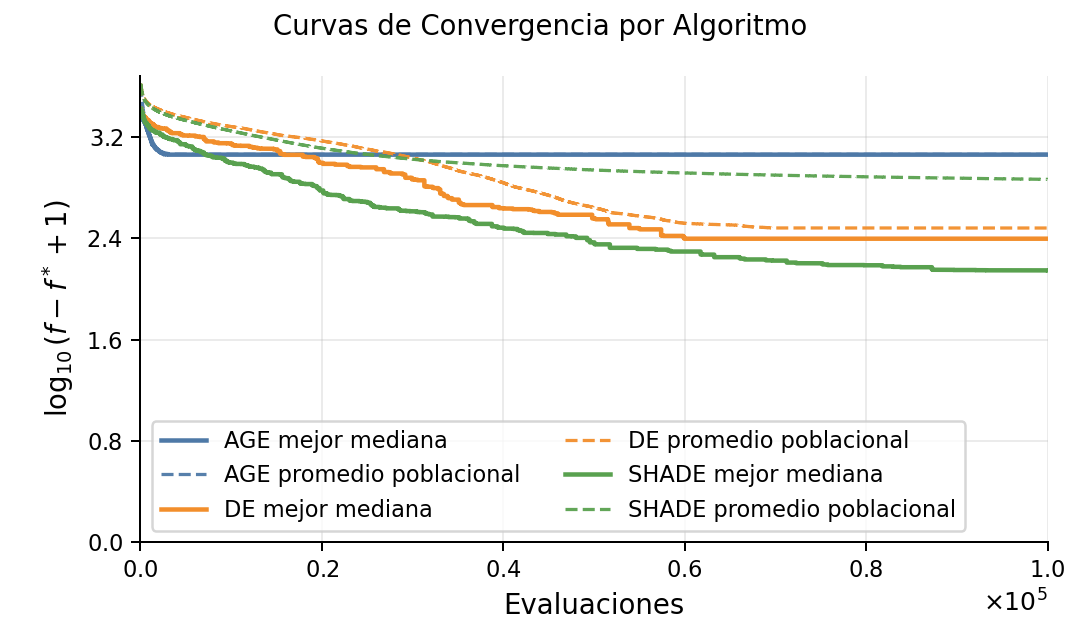
\includegraphics[width=\textwidth]{figuras/plots_sin_reinicio/curva_convergencia_cec2017_f10.png}
        \caption{\(f_{10}\)}
        \label{fig:convergencia_sin_reinicio_f10}
    \end{subfigure}

    \vspace{0.4cm}

    \begin{subfigure}[t]{0.8\textwidth}
        \centering
        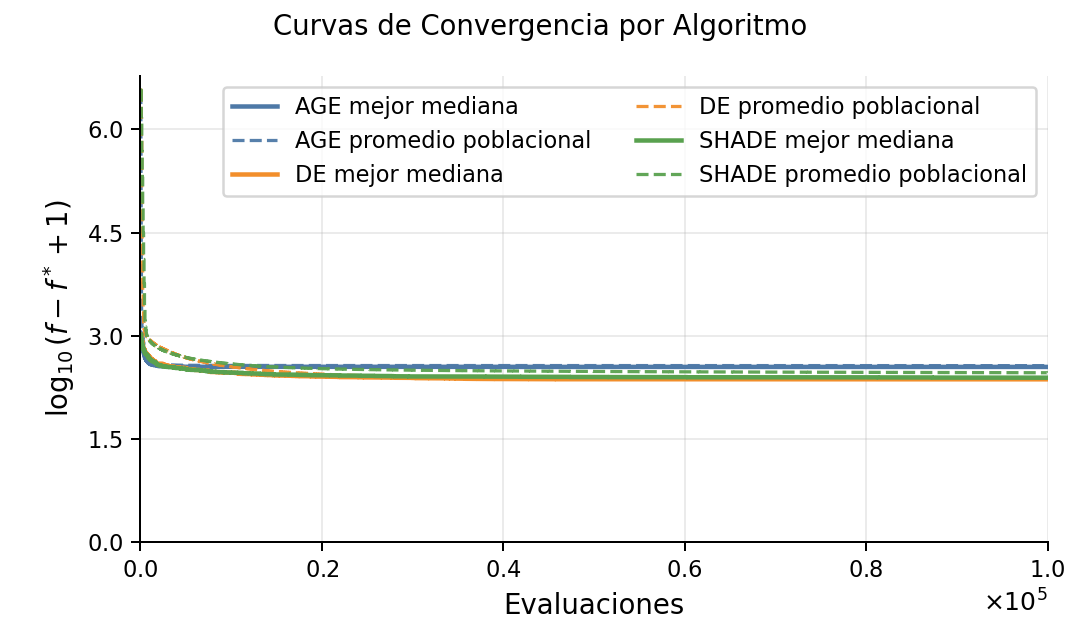
\includegraphics[width=\textwidth]{figuras/plots_sin_reinicio/curva_convergencia_cec2017_f29.png}
        \caption{\(f_{29}\)}
        \label{fig:convergencia_sin_reinicio_f29}
    \end{subfigure}
    \caption{Curvas de convergencia promedio sin reinicio en tres funciones representativas de CEC2017.}
    \label{fig:convergencia_sin_reinicio}
\end{figure}

\begin{figure}[H]
    \centering
    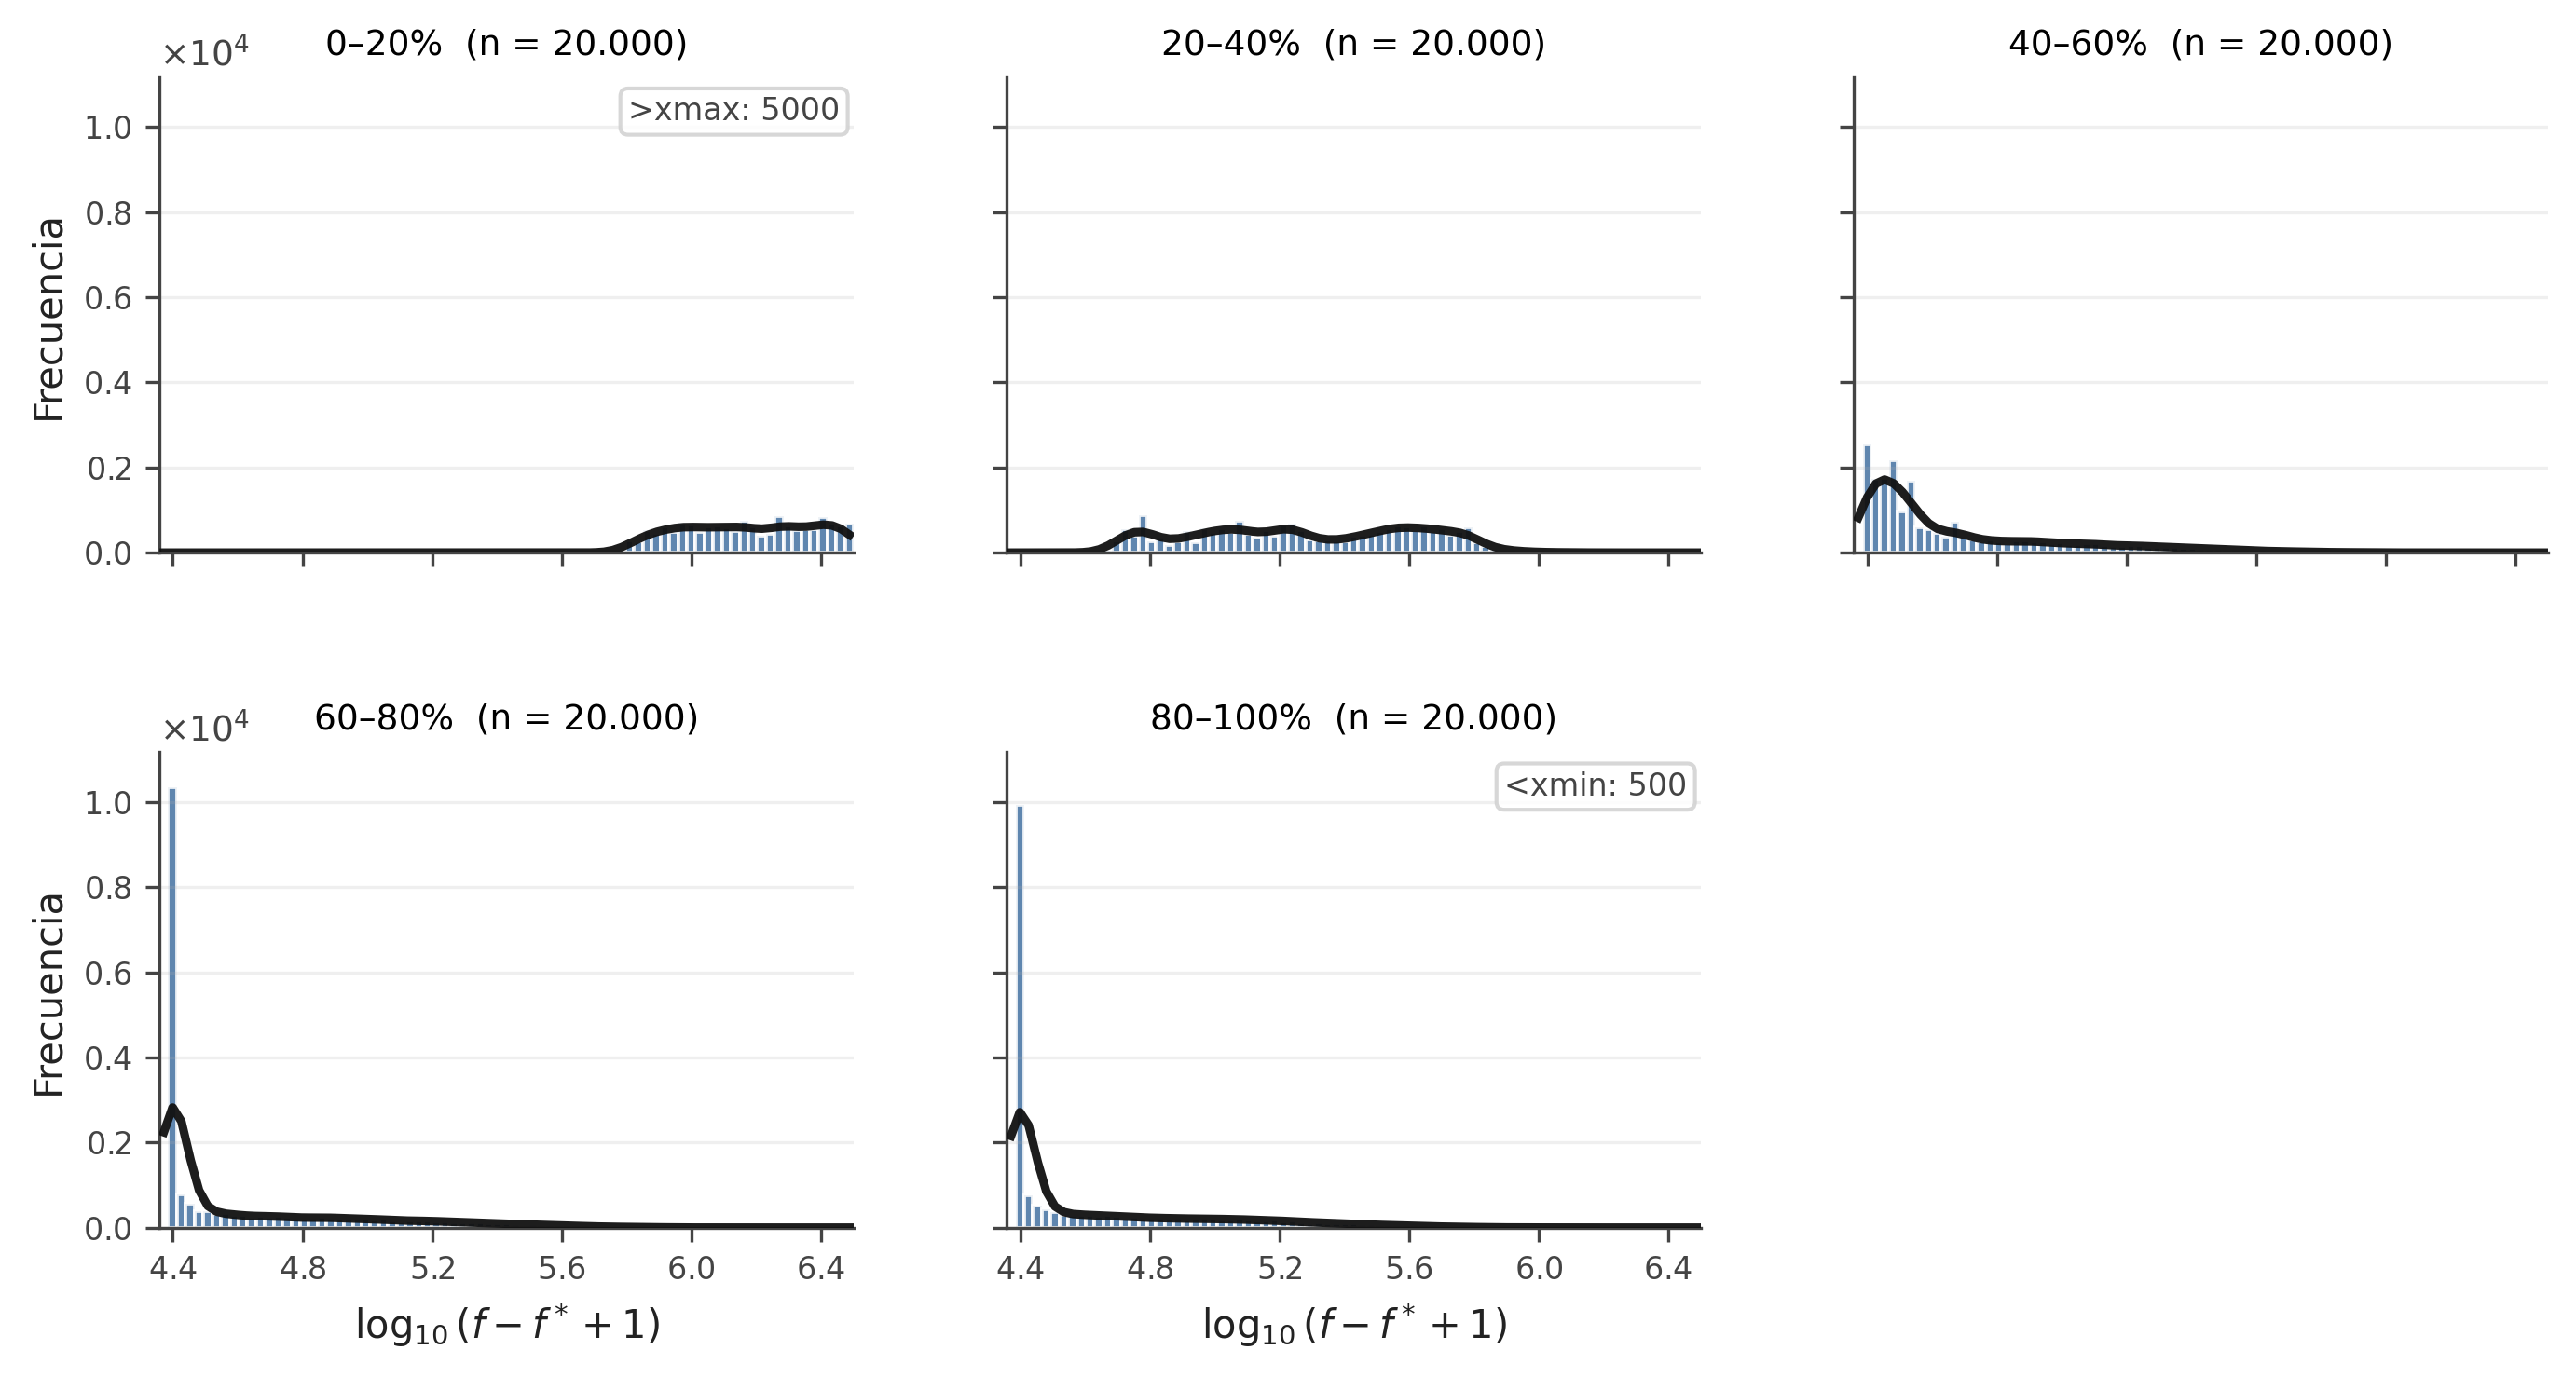
\includegraphics[width=1.0\textwidth]{figuras/plots_sin_reinicio/por_run/f12/age/sin_reinicio/histograma_fitness_fases_cec2017_f12_s41_sin_reinicio_age.png}
    \caption{Convergencia progresiva del error evaluada por bloques de la trayectoria: AGE sobre \(f_{12}\) (semilla 41).}
    \label{fig:bloques_sin_reinicio}
\end{figure}


Para evitar que las trayectorias queden dominadas por estas fases de estancamiento, se incorpora el criterio de reinicio elitista descrito en el Capítulo~\ref{chap:algo_tecnicas_ref}. A continuación, se evalúan las distintas configuraciones propuestas en el Capítulo~\ref{chap:metodologia_experimental} de dicho criterio con el objetivo de identificar, para cada metaheurística, aquella que mejor equilibre la reactivación de la búsqueda con la preservación de la calidad final de las soluciones.


% ------------------------------------------------------------
\subsection{Evaluación de las configuraciones de reinicio}
\label{subsec:evaluacion_reinicio}
% ------------------------------------------------------------

Una vez visualizado el problema del estancamiento, el objetivo no es establecer una clasificación global entre AGE, DE y SHADE, sino determinar si alguna configuración con reinicio resulta adecuada para generar las trayectorias que utilizarán posteriormente los modelos subrogados en las estrategias \textit{offline} y \textit{online}. En particular, se busca una configuración que reduzca el estancamiento sin introducir deterioros importantes en la calidad final.

Como punto de partida, se analiza si es posible seleccionar una única ventana de estancamiento común para las tres metaheurísticas. Adoptar una configuración global reduciría el riesgo de ajustar el criterio de reinicio de forma específica a un algoritmo concreto o al propio banco de problemas CEC2017. Para ello, se comparan las configuraciones definidas en el
Capítulo~\ref{chap:metodologia_experimental}: ventanas del \(1\%\), \(3\%\),
\(5\%\), \(7\%\) y \(10\%\) del presupuesto total de evaluaciones, junto con la versión sin reinicio.

Para cada metaheurística se consideran cuatro configuraciones:

\begin{table}[H]
    \centering
    \begin{tabular}{llc}
        \toprule
        \textbf{Configuración} & \textbf{Descripción}       & \textbf{Ventana de estancamiento} \\
        \midrule
        ALG                    & Sin reinicio               & --                                \\
        ALG-1                  & Reinicio con \(\rho=0.01\) & 1.000 evaluaciones                \\
        ALG-3                  & Reinicio con \(\rho=0.03\) & 3.000 evaluaciones                \\
        ALG-5                  & Reinicio con \(\rho=0.05\) & 5.000 evaluaciones                \\
        ALG-7                  & Reinicio con \(\rho=0.07\) & 7.000 evaluaciones                \\
        ALG-10                 & Reinicio con \(\rho=0.10\) & 10.000 evaluaciones               \\
        \bottomrule
    \end{tabular}
    \caption[Configuraciones genéricas de reinicio consideradas para cada metaheurística.]{Configuraciones genéricas de reinicio consideradas para cada metaheurística, donde \textbf{ALG} representa AGE, DE o SHADE.}
    \label{tab:configuraciones_reinicio_genericas}
\end{table}

Antes de analizar el impacto del reinicio, conviene evaluar empíricamente la agresividad del mecanismo. La Figura~\ref{fig:barplot_reinicios} muestra el número medio de reinicios activados por ejecución para cada configuración y metaheurística. Como era esperable, las ventanas de estancamiento menores provocan una activación más frecuente del mecanismo, por lo que esta información ayuda a interpretar los resultados posteriores sin sustituir a las comparaciones de calidad final.

\begin{figure}[htbp]
    \centering
    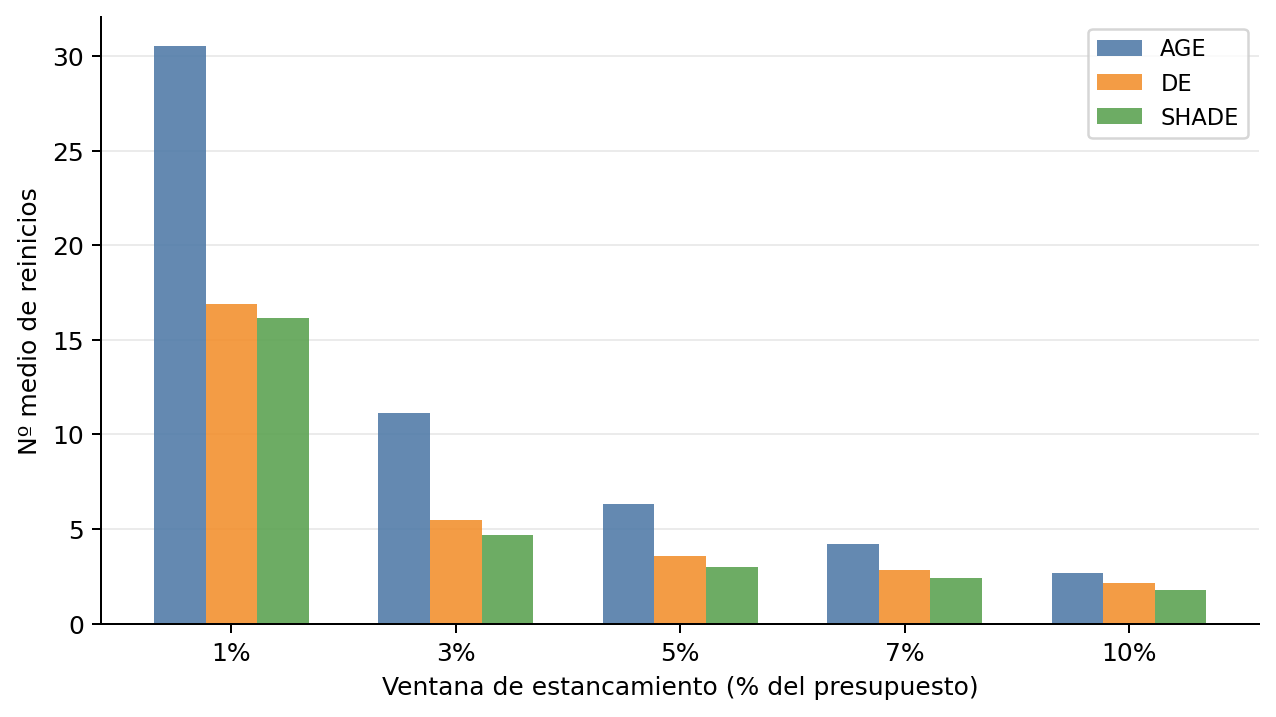
\includegraphics[width=0.9\textwidth]{figuras/barplot_reinicios_por_ventana_estancamiento.png}
    \caption{Número medio de reinicios elitistas por ejecución según la ventana de estancamiento \(\rho\).}
    \label{fig:barplot_reinicios}
\end{figure}

La selección final se apoya en las comparaciones de rendimiento generadas con
\textbf{TACOLAB}. Siguiendo el criterio metodológico definido en la
Sección~\ref{subsec:criterio_comparacion_modelos}, se prioriza el ranking medio calculado por TACOLAB, que permite resumir la posición relativa de cada
configuración sobre funciones con escalas de error heterogéneas. Las medias
del error final, recogidas en el Apéndice~\ref{ap:tablas_tacolab_reinicio}, se utilizan como apoyo complementario para comprobar que la configuración
seleccionada no introduce deterioros relevantes frente a la versión sin
reinicio.

Para estudiar esta evolución a lo largo de la ejecución, las Tablas~\ref{tab:ranking_reinicio_age}, \ref{tab:ranking_reinicio_de} y \ref{tab:ranking_reinicio_shade} muestran los rankings medios en distintos hitos del presupuesto de evaluaciones, siendo el 100\% el de mayor interés.

\begin{table}[H]
    \centering
    \footnotesize
    \setlength{\tabcolsep}{6pt}
    \renewcommand{\arraystretch}{0.95}
    \begin{tabular}{lccccc}
\toprule
\textbf{Configuración} & \multicolumn{5}{c}{\textbf{\% de evaluaciones}} \\
\cmidrule(lr){2-6}
{} & \textbf{20} & \textbf{40} & \textbf{60} & \textbf{80} & \textbf{100} \\
\midrule
AGE & 4.350 & 5.283 & 5.283 & 5.550 & 4.667 \\
AGE-1 & \textbf{1.783} & \textbf{1.350} & \textbf{1.600} & \textbf{1.333} & \textbf{1.600} \\
AGE-3 & 3.100 & 2.267 & 2.583 & 2.083 & 2.650 \\
AGE-5 & 3.517 & 3.667 & 3.400 & 3.350 & 3.367 \\
AGE-7 & 3.817 & 3.833 & 3.517 & 3.867 & 3.817 \\
AGE-10 & 4.433 & 4.600 & 4.617 & 4.817 & 4.900 \\
\bottomrule
\end{tabular}

    \caption{Ranking medio de TACOLAB para AGE en distintos hitos del presupuesto de evaluaciones.}
    \label{tab:ranking_reinicio_age}
\end{table}

\begin{table}[H]
    \centering
    \footnotesize
    \setlength{\tabcolsep}{6pt}
    \renewcommand{\arraystretch}{0.95}
    \begin{tabular}{lc}
\toprule
\textbf{Configuración} & \textbf{Rank medio (100\%)} \\
\midrule
DE-10 & \textbf{2.517} \\
DE-7 & 3.050 \\
DE-5 & 3.283 \\
DE-3 & 3.583 \\
DE & 4.017 \\
DE-1 & 4.550 \\
\bottomrule
\end{tabular}

    \caption{Ranking medio de TACOLAB para DE en distintos hitos del presupuesto de evaluaciones.}
    \label{tab:ranking_reinicio_de}
\end{table}

\begin{table}[H]
    \centering
    \footnotesize
    \setlength{\tabcolsep}{6pt}
    \renewcommand{\arraystretch}{0.95}
    \begin{tabular}{lccccc}
\toprule
\textbf{Configuración} & \multicolumn{5}{c}{\textbf{\% de evaluaciones}} \\
\cmidrule(lr){2-6}
{} & \textbf{20} & \textbf{40} & \textbf{60} & \textbf{80} & \textbf{100} \\
\midrule
SHADE & 3.200 & 3.083 & 3.033 & 3.267 & 3.550 \\
SHADE-1 & 4.600 & 4.450 & 4.517 & 4.583 & 4.583 \\
SHADE-3 & 4.000 & 3.917 & 3.883 & 3.750 & 3.717 \\
SHADE-5 & 3.183 & 3.633 & 3.583 & 3.450 & 3.283 \\
SHADE-7 & \textbf{2.883} & 3.167 & 3.250 & 3.117 & 2.950 \\
SHADE-10 & 3.133 & \textbf{2.750} & \textbf{2.733} & \textbf{2.833} & \textbf{2.917} \\
\bottomrule
\end{tabular}

    \caption{Ranking medio de TACOLAB para SHADE en distintos hitos del presupuesto de evaluaciones.}
    \label{tab:ranking_reinicio_shade}
\end{table}

El análisis de estos datos revela que el impacto del reinicio y la ventana evaluada no es uniforme entre los distintos algoritmos. Para aquellas ventanas muy pequeñas, correspondientes al 1\% y 3\% del presupuesto, se produce un escenario de reactivación muy frecuente donde, para un algoritmo como AGE, esta regeneración constante resulta adecuada, siendo AGE-1 la clara ganadora en la comparación por media final, con el mejor resultado en 25 de las 30 funciones y obteniendo el mejor ranking en todos los hitos. En cambio, este mismo patrón no se reproduce en DE ni en SHADE (véase en la Figura~\ref{fig:reinicio_shade_f10}). Las configuraciones con ventanas del 1\% se colocan en los peores puestos desde el inicio al ser ser metaheurísticas que requieren un mayor margen de evaluaciones para explotar la información acumulada en la población antes de que resulte conveniente reactivar la búsqueda (véase en la Figura~\ref{fig:convergencia_sin_reinicio}).

A medida que aumenta la ventana de estancamiento, el comportamiento cambia y las mejoras y empeoramientos vistos en las ventanas anteriores se pronuncian aún más. En DE y SHADE, las ventanas largas permiten preservar durante más tiempo la dinámica de búsqueda y conducen a los mejores rankings finales, especialmente con la configuración del 10\%. Por el contrario, en AGE una ventana tan amplia ralentiza su capacidad de respuesta, donde AGE-10 obtiene incluso un peor ranking final que la variante sin reinicio. Por tanto, no existe una ventana óptima común para las tres metaheurísticas ya que la configuración adecuada depende de la dinámica de búsqueda propia de cada algoritmo.

Esta clara diferencia de necesidades se refleja visualmente en la Figura~\ref{fig:rendimiento_agregado_malla}, que confirma el análisis extraído de las tablas comparativas: la curva de AGE se deteriora a medida que la ventana se hace más grande, mientras que las trayectorias de DE y SHADE mejoran progresivamente hasta alcanzar su punto óptimo en los valores más altos.

\begin{figure}[htbp]
    \centering
    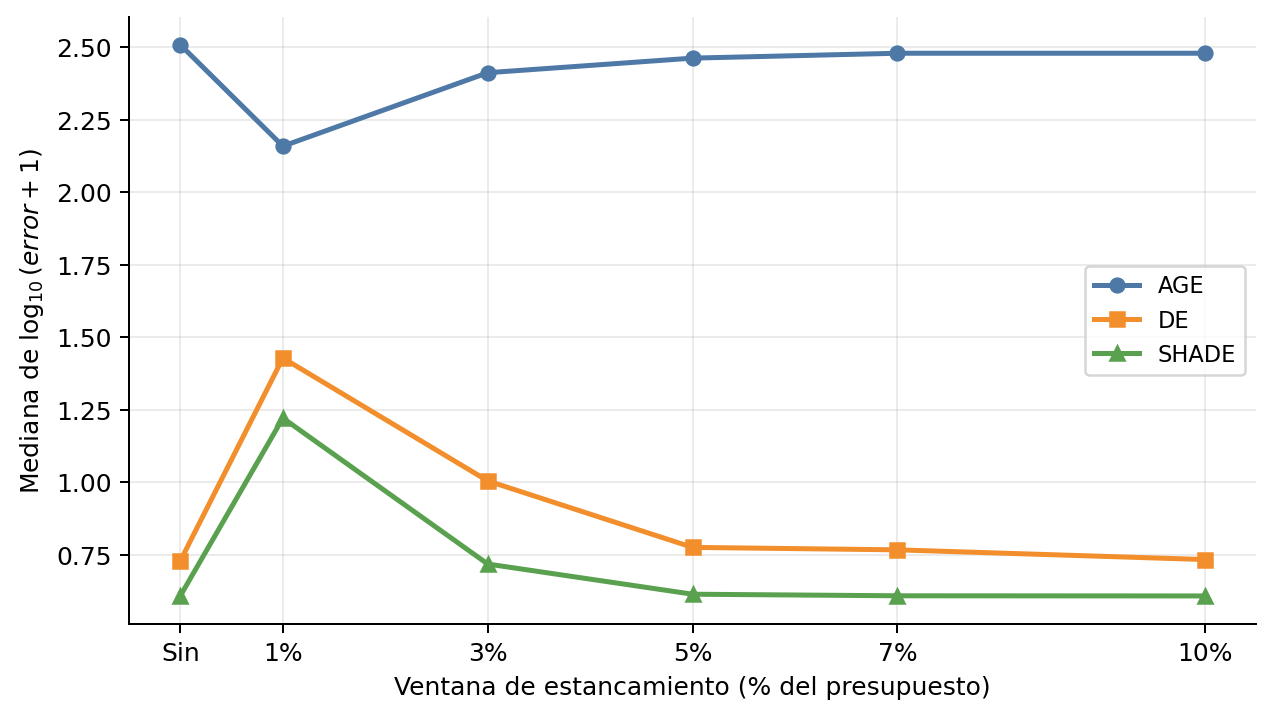
\includegraphics[width=0.95\textwidth]{figuras/rendimiento_por_ventana_estancamiento.png}
    \caption{Evolución del rendimiento agregado en función del tamaño de la ventana de estancamiento \(\rho\).}
    \label{fig:rendimiento_agregado_malla}
\end{figure}

\begin{figure}[htbp]
    \centering
    \begin{subfigure}{0.95\textwidth}
        \centering
        
\includegraphics[width=\textwidth]{figuras/reinicio/curva_convergencia_reinicio_cec2017_f10_shade.png}
        \caption{Convergencia}
    \end{subfigure}
    \hfill
    \begin{subfigure}{0.95\textwidth}
        \centering
        
\includegraphics[width=\textwidth]{figuras/reinicio/curva_diversidad_reinicio_cec2017_f10_shade.png}
        \caption{Diversidad}
    \end{subfigure}
    \caption{Ejemplo de reinicio en SHADE sobre \(f_{10}\) con \(\rho=0.01\).}
    \label{fig:reinicio_shade_f10}
\end{figure}



% ============================================================
\subsection{Conclusiones sobre la reactivación de la búsqueda}
\label{subsec:conclusiones_reinicio_parcial}
% ============================================================

%% deberiamos decidir en esta si se usa ventana común o específica, justificandolo con los resultados.

%% si finalmente elegimos ventanas distintas, tenemos que explicarlo como una excepcion motivada por los datos, no como punto de partida.

A partir del análisis anterior, los resultados dejan claro que es inviable utilizar una única ventana de estancamiento común para todas las metaheurísticas.

Por tanto, las configuraciones más adecuadas para cada algoritmo son:

\begin{table}[H]
    \centering
    \small
    \begin{tabular}{lc}
        \toprule
        \textbf{Algoritmo} & \textbf{Configuración} \\
        \midrule
        AGE                & AGE-1                  \\
        DE                 & DE-10                  \\
        SHADE              & SHADE-10               \\
        \bottomrule
    \end{tabular}
    \caption{Configuraciones seleccionadas para la generación de trayectorias en la fase de subrogados.}
    \label{tab:configuraciones_reinicio_seleccionadas}
\end{table}

Con las configuraciones fijadas, la siguiente fase evalúa las estrategias de entrenamiento \textit{offline} de los modelos subrogados sobre trayectorias menos dominadas por estancamiento y, por tanto, más adecuadas para analizar la capacidad predictiva de los modelos.

\section{Estudio offline: técnicas \textit{subrogadas} y configuración de entrenamiento}
\label{sec:estudio_offline}

% Siguiendo el protocolo descrito en la
% Sección~\ref{subsec:funciones_cribado_offline}, la comparativa inicial se
% realiza sobre el subconjunto representativo de funciones seleccionado para
% la fase de cribado.

Esta sección tiene como objetivo determinar empíricamente qué combinación de modelo subrogado y estrategia de entrenamiento ofrece el mejor compromiso entre fidelidad ordinal, precisión métrica y eficiencia computacional. Para ello, se comparan de forma \textit{offline} las técnicas consideradas y las estructuras de aprendizaje definidas en el Capítulo \ref{chap:algo_tecnicas_ref}, utilizando para el entrenamiento las trayectorias históricas generadas por las configuraciones finales de las metaheurísticas seleccionadas.

Siguiendo el protocolo definido en la
Subsección~\ref{subsec:funciones_cribado_offline}, la comparación inicial de modelos se realiza sobre el subconjunto representativo de funciones seleccionado para el cribado \textit{offline}, manteniendo las \(51\) semillas empleadas en la generación de trayectorias.

\subsection{Viabilidad Computacional y Estrategia Global}
\label{subsec:viabilidad_estrategia_global}

De cara a la futura integración \textit{online}, el coste computacional es muy relevante, especialmente el \textbf{tiempo de entrenamiento y predicción}. En este sentido, al llevar a cabo la ejecución de los distintos modelos de Aprendizaje Automático aplicados como técnicas de subrogado, el modelo \textit{Support Vector Regression} (SVR) evidenció limitaciones significativas dependiendo de la estrategia de entrenamiento empleada.

Mientras que el volumen de datos se mantiene constante en bloques fijos del 20 \% del presupuesto para la estrategia no acumulativa, mantener un historial de muestras cuyo tamaño incrementa en cada paso cronológico como conjunto de entrenamiento descarta a SVR de la estrategia acumulativa. Al escalar su complejidad de forma no lineal ($\mathcal{O}(N^3)$) respecto al número de muestras, el tiempo de ejecución se volvió desconsiderado para cualquier función (vease en la Figura \ref{fig:viabilidad_svr_f4}).

\begin{figure}[htbp]
    \centering
    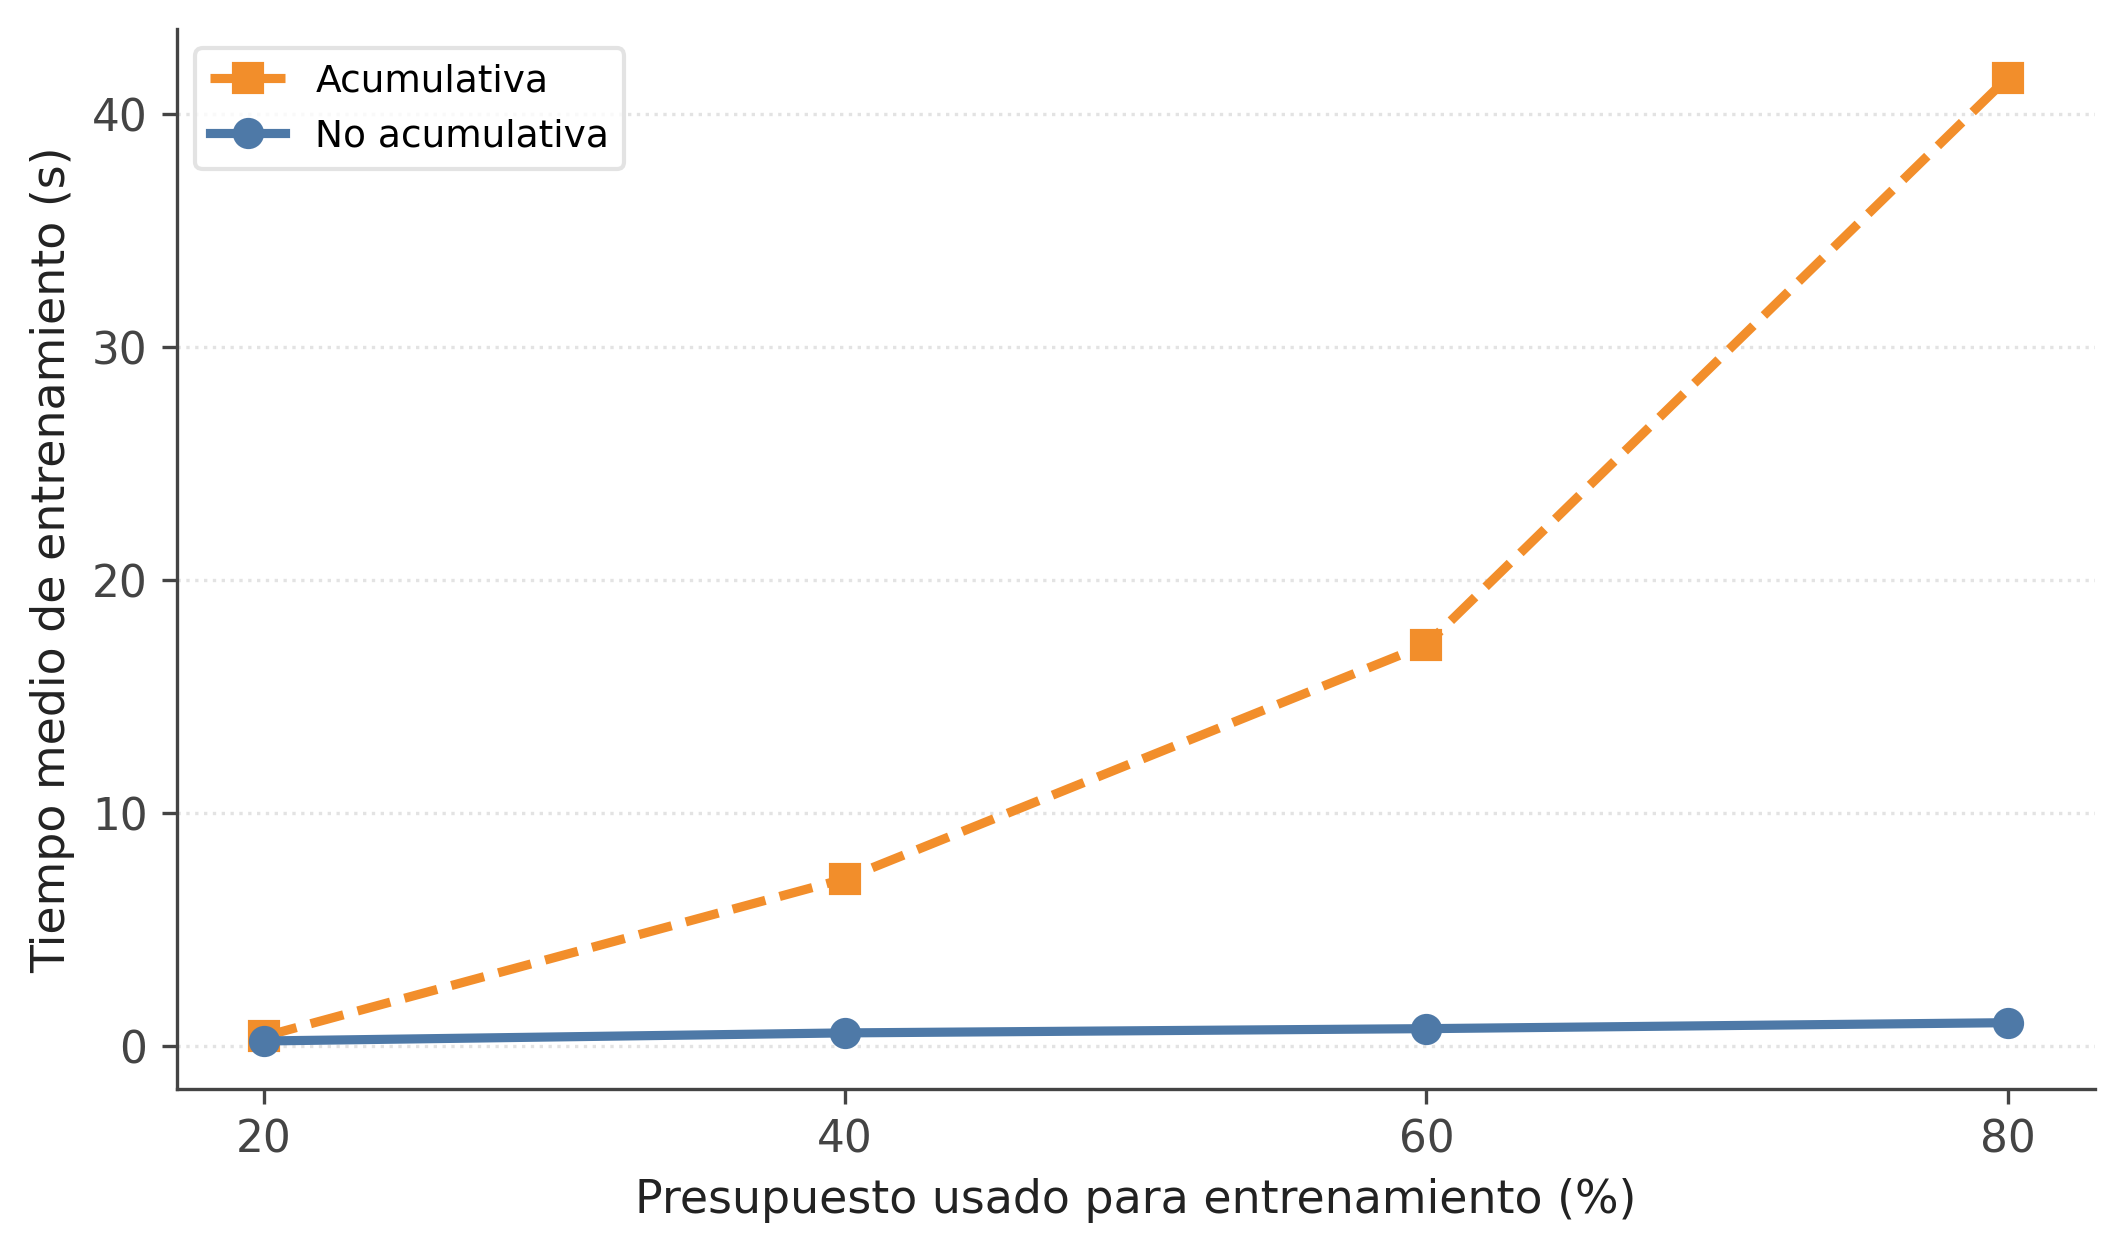
\includegraphics[width=0.9\textwidth]{figuras/surrogates_offline/viabilidad_svr_tiempo_entrenamiento_f4.png}
    \caption{Evolución del tiempo medio de entrenamiento de SVR sobre \(f_4\) para las estrategias acumulativa y no acumulativa.}
    \label{fig:viabilidad_svr_f4}
\end{figure}

Para garantizar una comparación justa, los resultados globales de ambas estrategias presentados en esta sección se han computado agregando de forma exclusiva los modelos que finalizaron exitosamente ambas configuraciones.

% \begin{table}[H]
    \centering
    \begin{tabular}{lrrrrr}
        \toprule
        \textbf{Estrategia} & \textbf{Spearman} & \textbf{nMAE} & \textbf{nRMSE} & \textbf{Entren. (s)} \\
        \midrule
        Acumulativo         & 0.1911            & 506.7963      & 546.1524       & 1.444                \\
        No acumulativo      & 0.2517            & 273.8175      & 309.3682       & 0.687                \\
        \bottomrule
    \end{tabular}
    \caption[Comparativa global de rendimiento entre estrategias \textit{offline}.]{Comparativa global de rendimiento entre estrategias \textit{offline} promediando todas las funciones, semillas y metaheurísticas (basada en los 6 modelos comunes).}
    \label{tab:comparativa_estrategias_offline}
\end{table}
\begin{table}[H]
    \centering
    \small
    \begin{adjustbox}{max width=\textwidth}
\begin{tabular}{l r r r r r}
\toprule
\textbf{Algoritmo} & \textbf{Vict. no\_acum (\%)} & \textbf{Spearman no\_acum} & \textbf{Spearman acum} & \textbf{Entren. no\_acum (s)} & \textbf{Entren. acum (s)} \\
\midrule
AGE & 65.1\% & \textbf{0.5145} & 0.2119 & 0.2798 & 1.1537 \\
DE & 66.7\% & \textbf{0.2063} & 0.0624 & 0.4834 & 1.6325 \\
SHADE & 59.5\% & \textbf{0.3946} & 0.3065 & 0.4581 & 1.6465 \\
\bottomrule
\end{tabular}
    \end{adjustbox}
    \caption{Comparativa de estrategias \textit{offline} por algoritmo. Victorias: porcentaje de combinaciones (función~$\times$~bloque~$\times$~modelo) en las que la estrategia no acumulativa supera a la acumulativa en Spearman.}
    \label{tab:comparativa_estrategias_offline_v2}
\end{table}

Los resultados agregados de la Tabla~\ref{tab:comparativa_estrategias_offline} muestran una ventaja clara de la estrategia no acumulativa frente a la acumulativa. En concreto, la estrategia no acumulativa obtiene un valor medio de Spearman superior y logra reducir casi a la mitad tanto los errores normalizados como los tiempos de cómputo.

Este comportamiento confirma los riesgos de mezclar muestras procedentes de fases anteriores, ya que aumenta el tamaño del conjunto de entrenamiento sin garantizar que aporten información útil para predecir el bloque futuro inmediato.

Para comprobar que esta conclusión no se debe únicamente al comportamiento
agregado de la tabla, la Figura~\ref{fig:evolucion_spearman_bloques_offline}
muestra la evolución del coeficiente de Spearman a lo largo de los bloques
temporales evaluados.

% \begin{figure}[htbp]
%     \centering
%     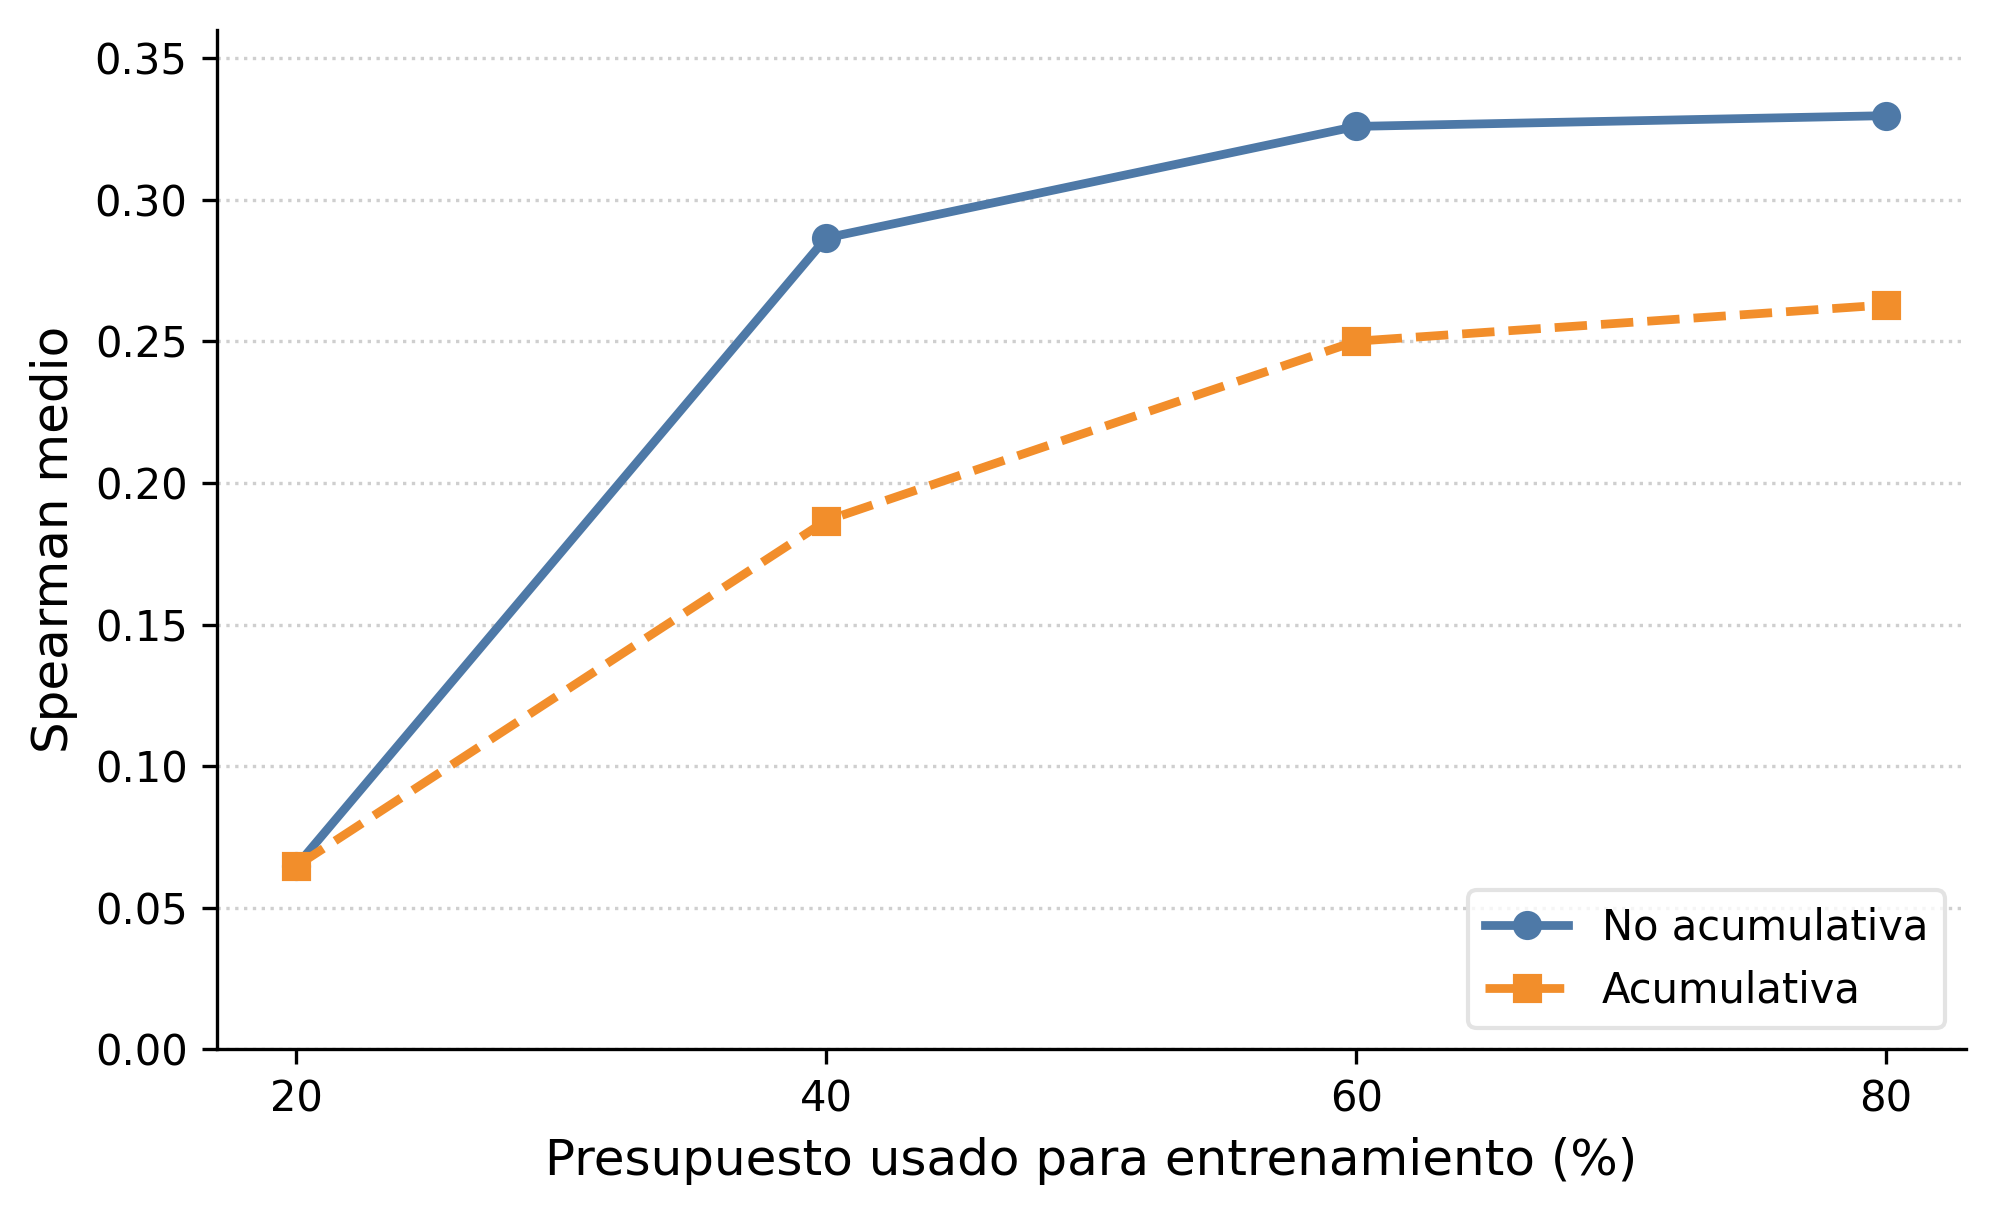
\includegraphics[width=0.8\textwidth]{figuras/surrogates_offline/evolucion_spearman_por_bloque_sin_svr.png}
%     \caption[Evolución de la correlación de Spearman media por bloque temporal para las estrategias acumulativa y no acumulativa.]{Evolución de la correlación de Spearman media por bloque temporal para las estrategias acumulativa y no acumulativa, excluyendo SVR por no completar la evaluación acumulativa.}
%     \label{fig:evolucion_spearman_bloques_offline}
% \end{figure}
\begin{figure}[H]
    \centering
    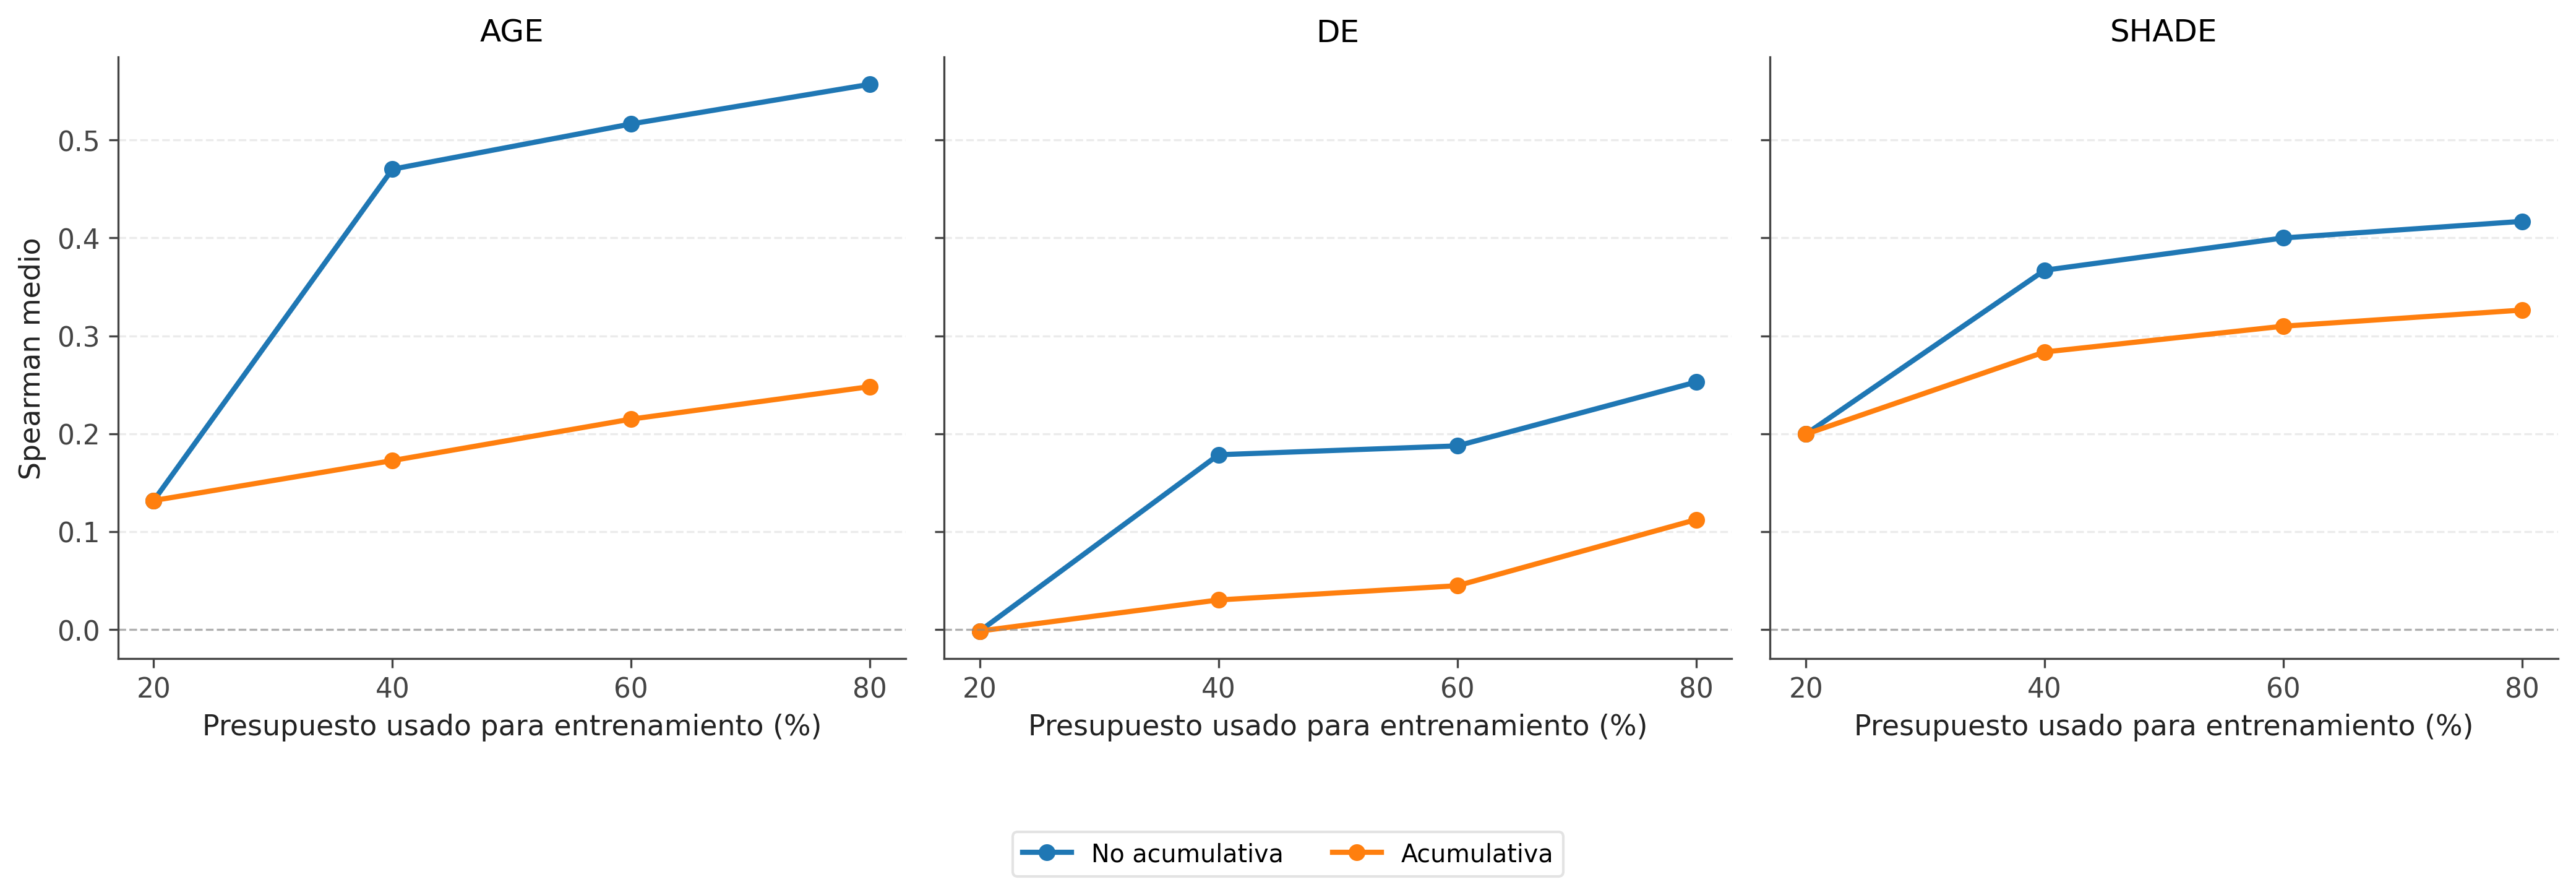
\includegraphics[width=\textwidth]{figuras/surrogates_offline/evolucion_spearman_por_bloque_por_algoritmo.png}
    \caption[Evolución de la correlación de Spearman media por bloque temporal para las estrategias acumulativa y no acumulativa.]{Evolución de la correlación de Spearman media por bloque temporal para las estrategias acumulativa y no acumulativa, desglosada por algoritmo (AGE, DE, SHADE).}
    \label{fig:evolucion_spearman_bloques_offline}
\end{figure}

La Figura~\ref{fig:evolucion_spearman_bloques_offline} confirma que la ventaja de la estrategia no acumulativa no procede de un único bloque temporal. En el primer bloque ambas estrategias parten de valores prácticamente idénticos, ya que el conjunto de entrenamiento disponible es equivalente. Sin embargo, a partir del segundo bloque la estrategia no acumulativa obtiene de forma consistente valores superiores de Spearman. Esta diferencia se mantiene hasta los bloques finales,
lo que indica que la ventaja observada en la tabla agregada no responde a un
comportamiento puntual, sino a una tendencia sostenida durante la evaluación.

Por tanto, el \textbf{enfoque no acumulativo} es la mejor opción al aislar al modelo de la influencia negativa del histórico y permitir que se concentre exclusivamente en la región temporal más reciente de la búsqueda. En consecuencia, los análisis posteriores se centran en la estrategia no acumulativa como protocolo de entrenamiento \textit{offline} de referencia.

\subsection{Competición de Modelos y Evolución por Bloques}
\label{subsec:comparacion_modelos}

Tras justificar la estrategia no acumulativa como protocolo de evaluación ideal, este apartado profundiza en el comportamiento individual de cada modelo a lo largo de la optimización, reincorporando al modelo SVR en la comparativa.

% La Figura~\ref{fig:evolucion_spearman_modelos_no_acumulativo} desglosa la evolución del coeficiente de Spearman para cada modelo bajo el esquema no acumulativo. Cada punto representa una evaluación temporal adelantada: el modelo se entrena con el último bloque disponible y se valida sobre el bloque inmediatamente posterior. Así, el punto situado en la cota del 60\% de presupuesto usado para entrenamiento corresponde al modelo ajustado con el tramo 40--60\% y validado sobre el bloque futuro 60--80\%.

La Figura~\ref{fig:evolucion_spearman_modelos_no_acumulativo} muestra cómo cambia la capacidad de ordenación de cada modelo conforme avanza la trayectoria. El primer punto corresponde al entrenamiento con el bloque inicial 0--20\% y la validación sobre el bloque 20--40\%, por lo que representa la primera situación en la que podría utilizarse un subrogado tras una fase inicial de muestreo. Los puntos posteriores permiten observar si esa capacidad de ordenación se mantiene, mejora o se degrada conforme la búsqueda avanza hacia regiones más concretas del espacio.


% \begin{figure}[H]
%     \centering
%     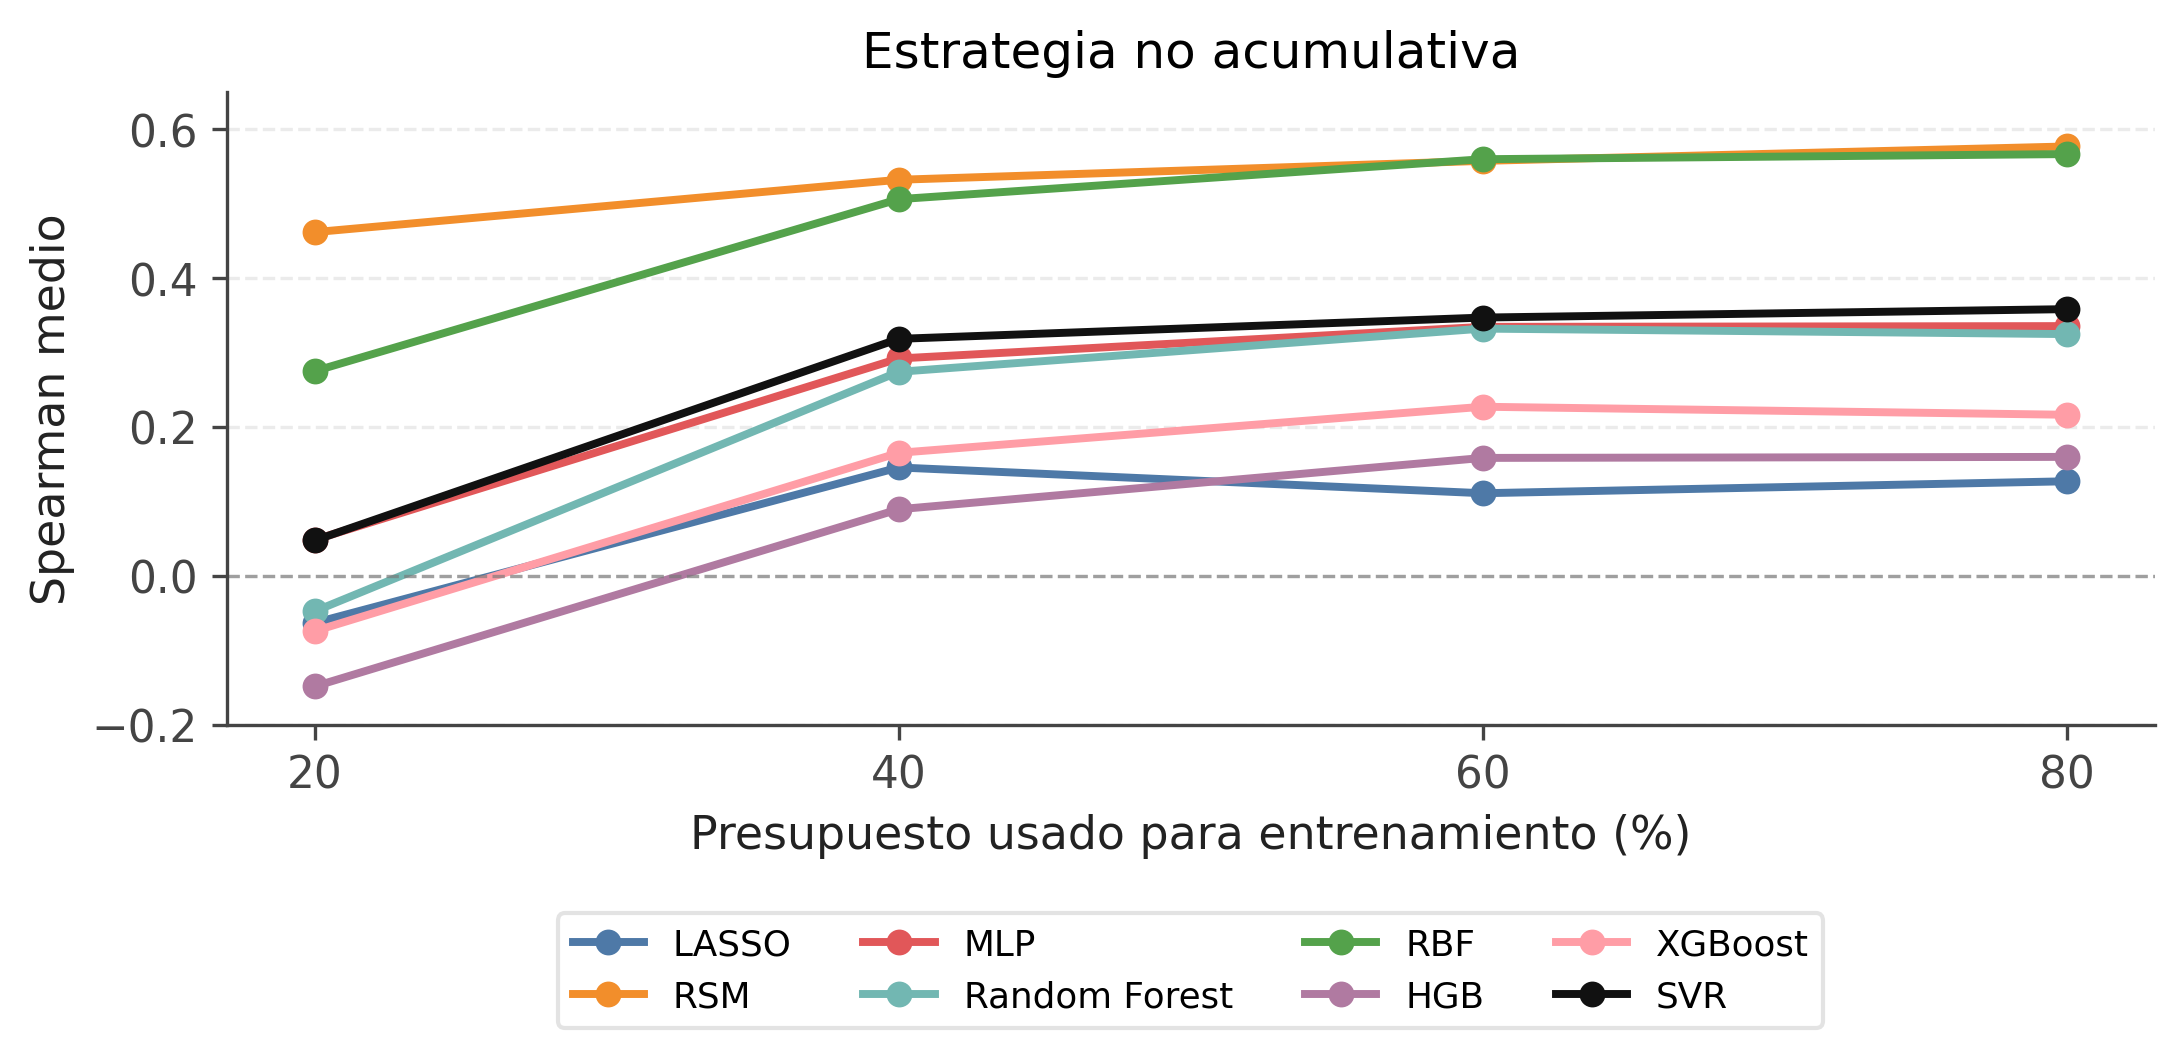
\includegraphics[width=1.0\textwidth]{figuras/surrogates_offline/evolucion_spearman_modelos_no_acumulativo.png}
%     \caption[Evolución de la correlación de Spearman media por bloques temporales bajo la estrategia no acumulativa.]{Evolución de la correlación de Spearman media por bloques temporales bajo la estrategia no acumulativa. Cada punto se obtiene entrenando con el bloque inmediatamente anterior al bloque evaluado.}
%     \label{fig:evolucion_spearman_modelos_no_acumulativo}
% \end{figure}
\begin{figure}[H]
    \centering
    \begin{subfigure}[b]{0.32\textwidth}
        \centering
        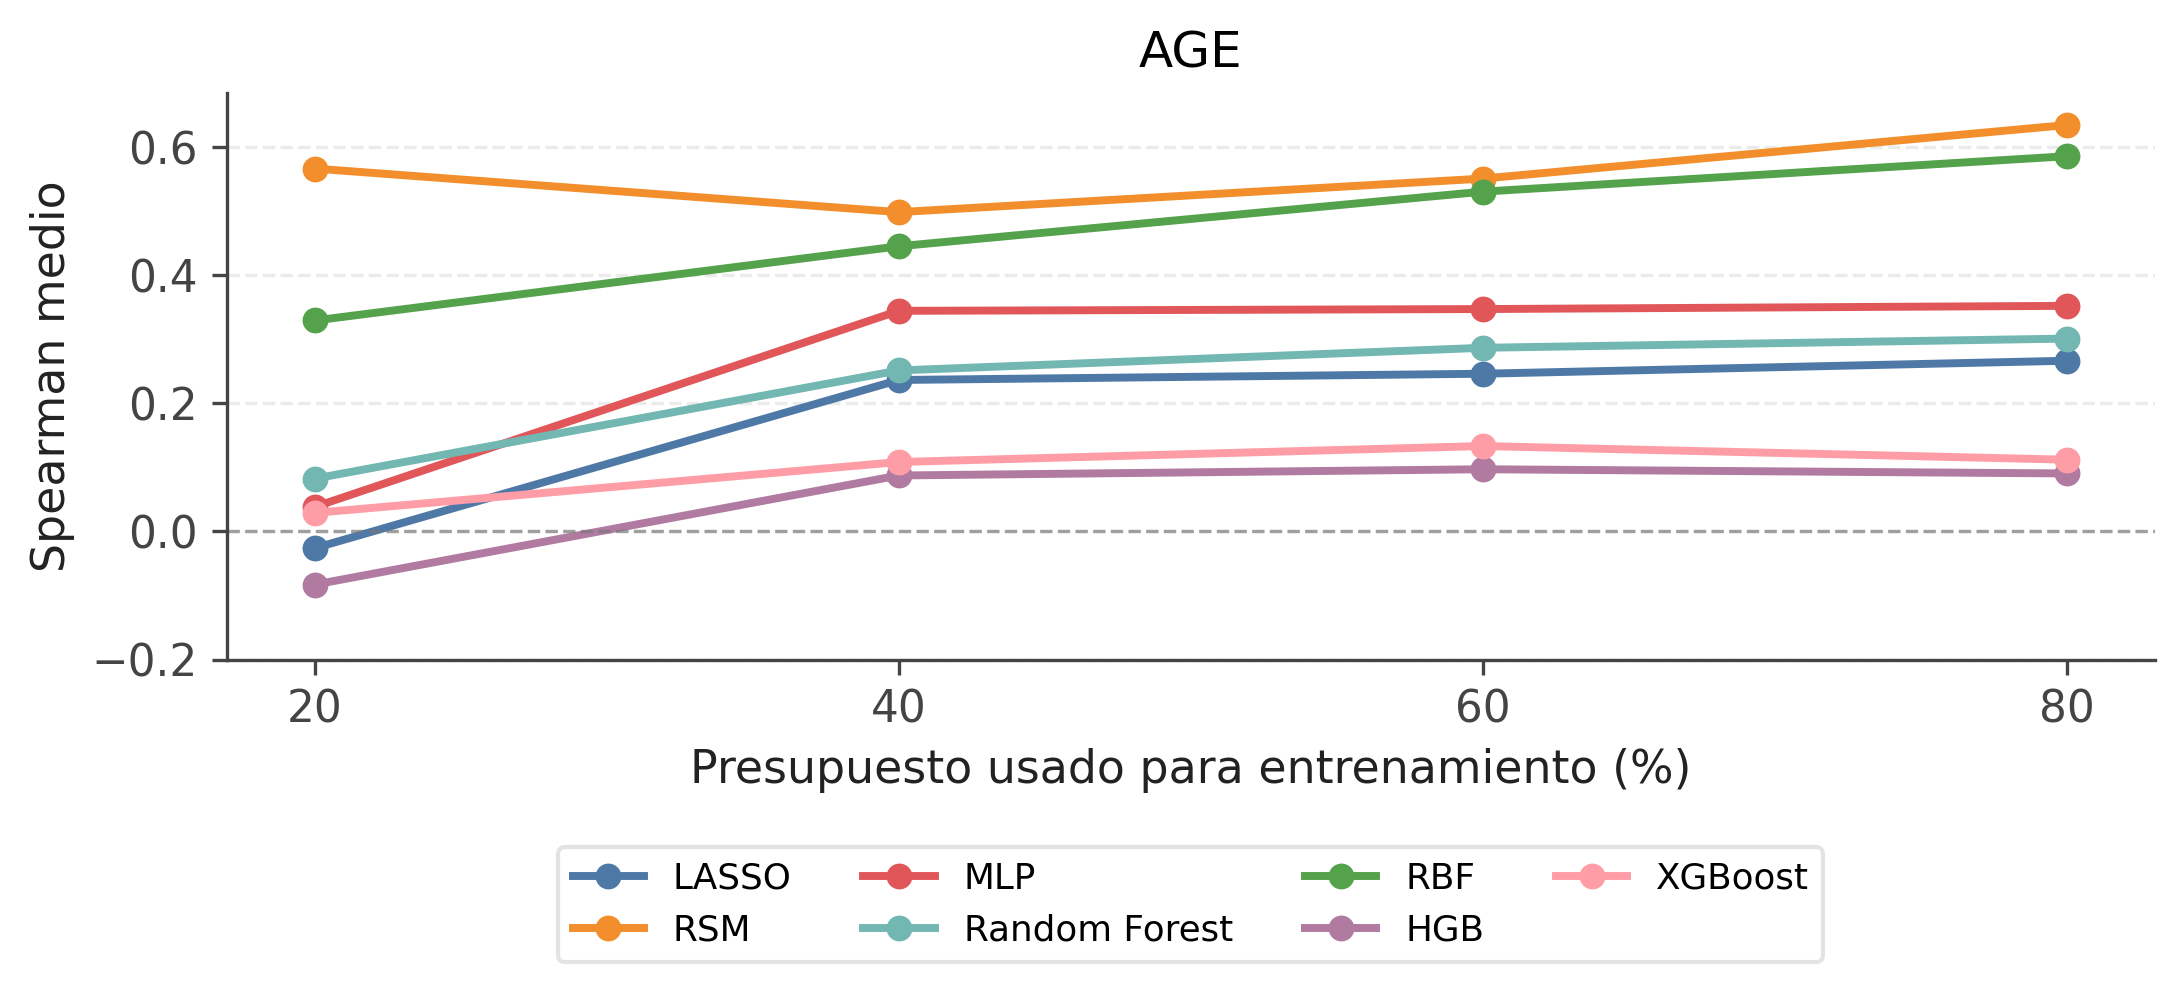
\includegraphics[width=\textwidth]{figuras/surrogates_offline/evolucion_spearman_modelos_no_acumulativo_age.png}
        \caption{AGE}
    \end{subfigure}
    \hfill
    \begin{subfigure}[b]{0.32\textwidth}
        \centering
        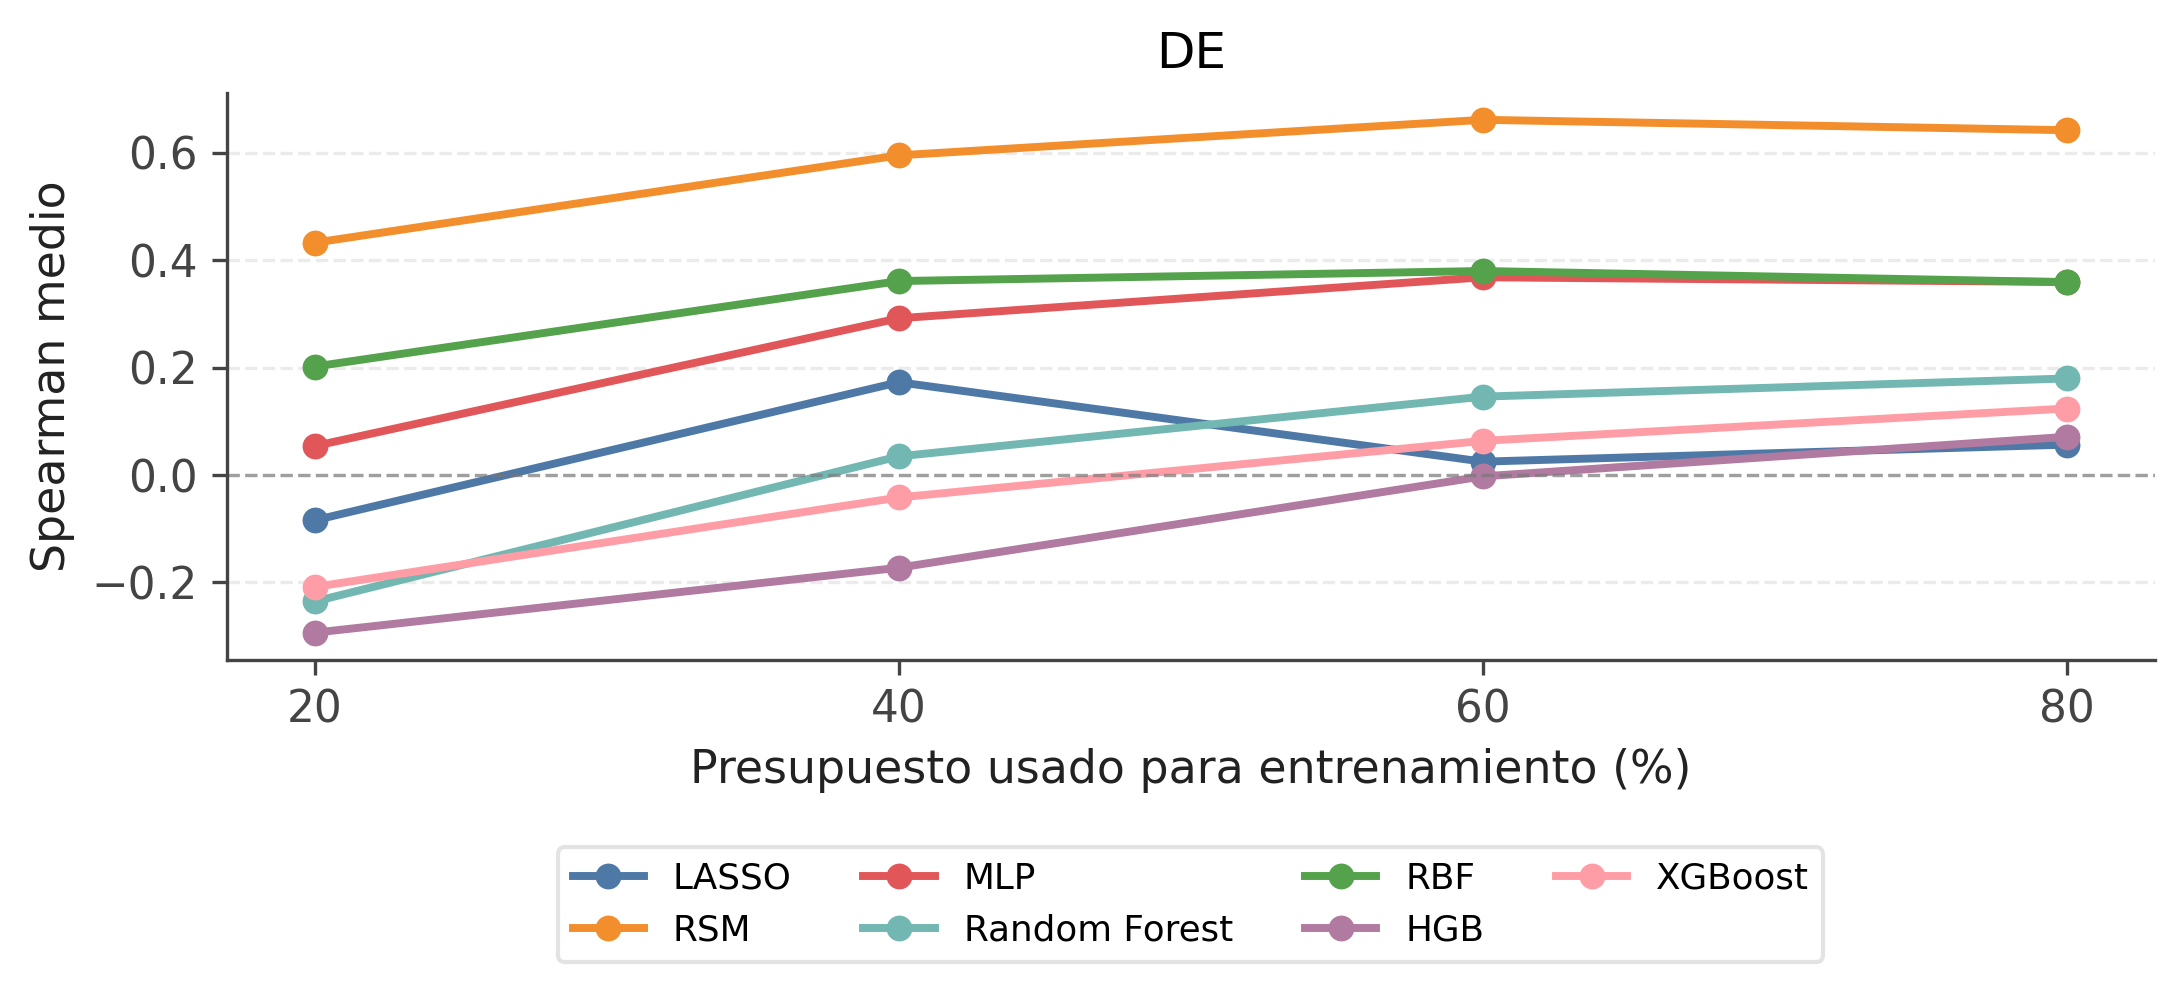
\includegraphics[width=\textwidth]{figuras/surrogates_offline/evolucion_spearman_modelos_no_acumulativo_de.png}
        \caption{DE}
    \end{subfigure}
    \hfill
    \begin{subfigure}[b]{0.32\textwidth}
        \centering
        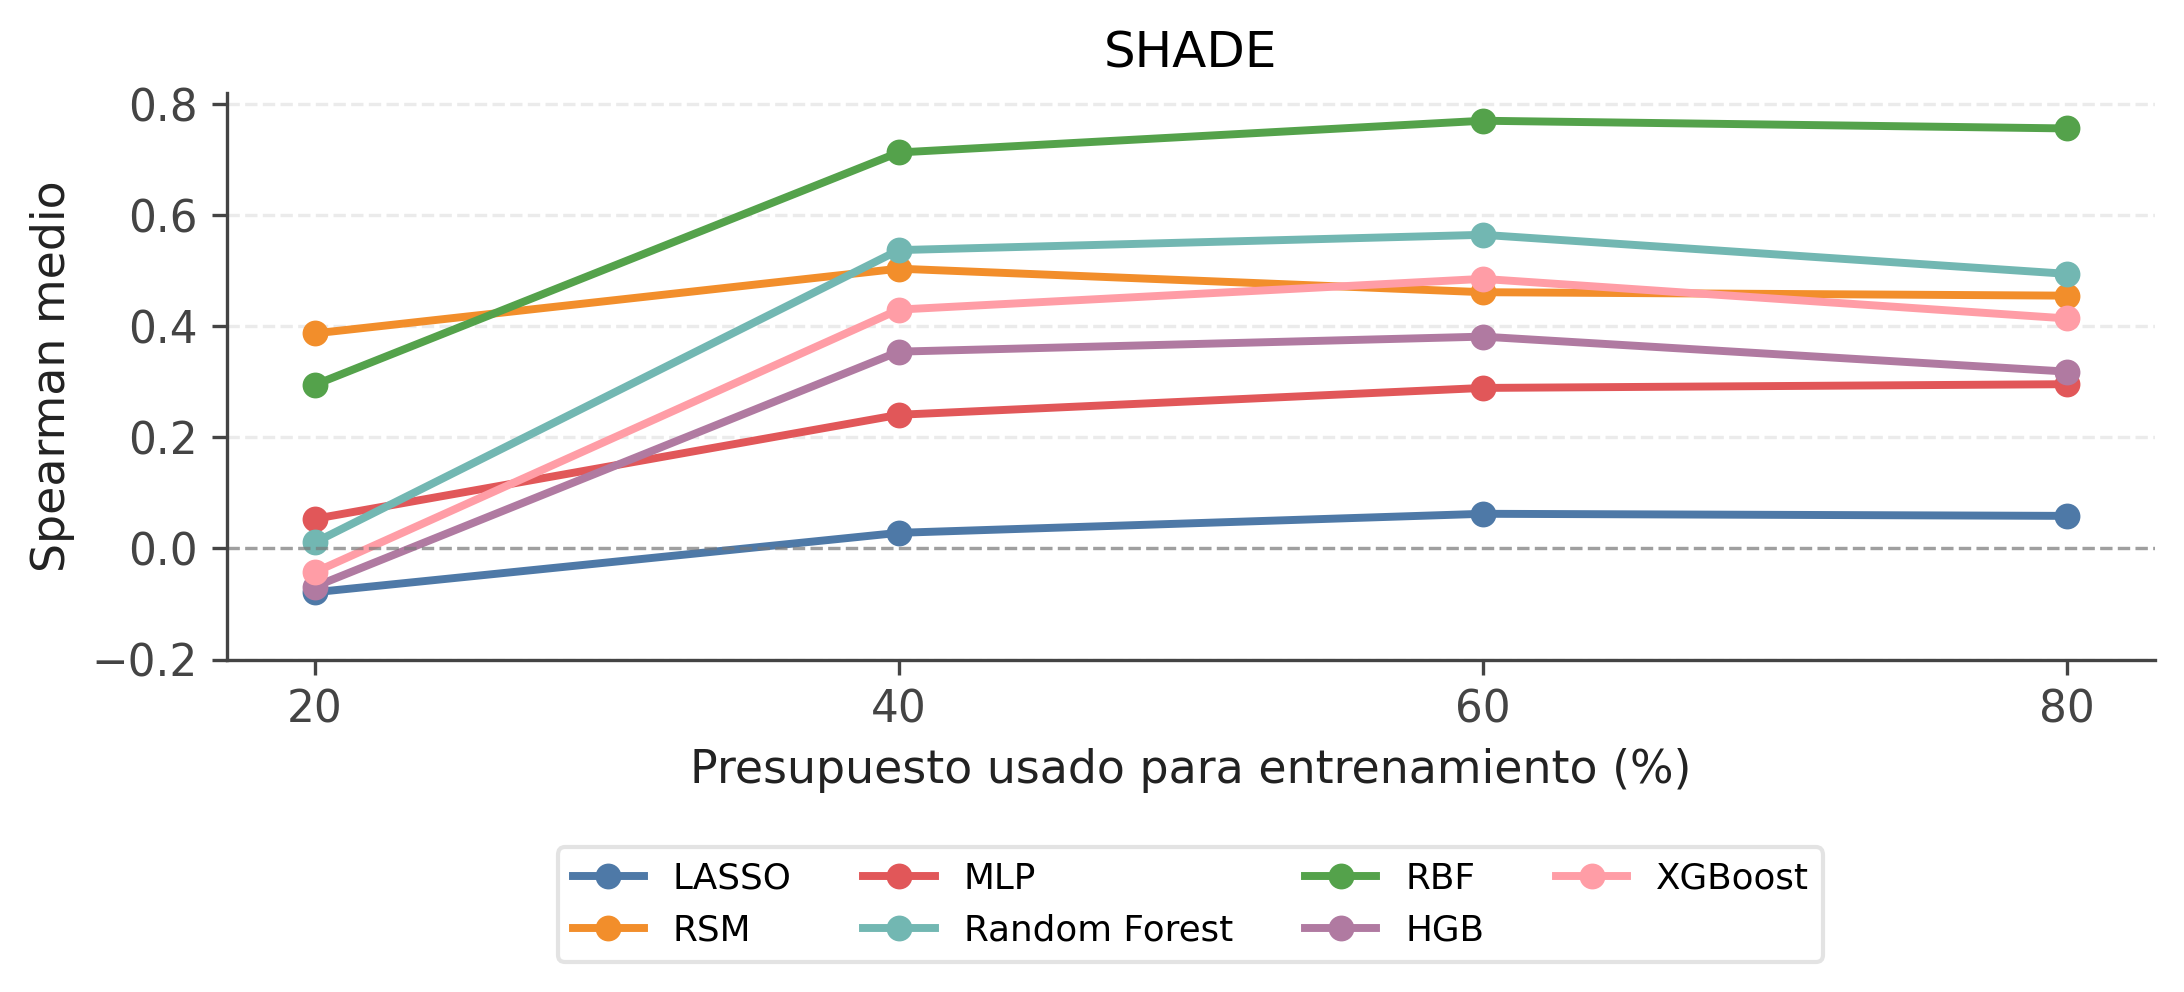
\includegraphics[width=\textwidth]{figuras/surrogates_offline/evolucion_spearman_modelos_no_acumulativo_shade.png}
        \caption{SHADE}
    \end{subfigure}
    \caption[Evolución de la correlación de Spearman media por bloques temporales bajo la estrategia no acumulativa.]{Evolución de la correlación de Spearman media por bloques temporales bajo la estrategia no acumulativa, desglosada por algoritmo. Cada punto se obtiene entrenando con el bloque inmediatamente anterior al bloque evaluado.}
    \label{fig:evolucion_spearman_modelos_no_acumulativo}
\end{figure}

Desde esta perspectiva temporal se observa una separación clara entre modelos. RSM parte con el mejor comportamiento desde el primer bloque y mantiene valores elevados durante toda la evaluación. RBF, en cambio, comienza con una correlación menor, pero mejora de forma marcada al pasar al bloque 40--60\% y, desde ese momento, se mantiene muy próximo a RSM. Esta evolución sugiere que RBF necesita trayectorias algo más estructuradas para explotar mejor la información local, mientras que RSM resulta más competitivo desde fases tempranas.

El resto de modelos también mejora respecto al primer bloque, pero su evolución se estabiliza en niveles claramente inferiores, destacando SVR, MLP o Random Forest. Por tanto, la figura no solo permite identificar qué modelos alcanzan mejores valores finales, sino también en qué momento de la trayectoria empiezan a ser útiles como aproximadores subrogados.

Las Tablas~\ref{tab:comparativa_modelos_bloques_age}, \ref{tab:comparativa_modelos_bloques_de} y \ref{tab:comparativa_modelos_bloques_shade} trasladan esa evolución a rangos concretos por bloque y algoritmo.

% \begin{table}[H]
    \centering
    \small
    \setlength{\tabcolsep}{5pt}
    \renewcommand{\arraystretch}{1.12}
    \begin{adjustbox}{max width=\textwidth}
        \begin{tabular}{l cccc ccc}
            \toprule
            \multirow{2}{*}{\textbf{Modelo}}
                             & \multicolumn{4}{c}{\textbf{Spearman por bloque de validación}}
                             & \multicolumn{3}{c}{\textbf{Media agregada}}                                                                                                                                 \\
            \cmidrule(lr){2-5} \cmidrule(lr){6-8}
                             & \textbf{20--40\%}
                             & \textbf{40--60\%}
                             & \textbf{60--80\%}
                             & \textbf{80--100\%}
                             & \textbf{nRMSE $\downarrow$}
                             & \textbf{Entren. $\downarrow$}
                             & \textbf{Pred. $\downarrow$}                                                                                                                                                 \\
            \midrule
            \rowcolor{gray!10}
            \textbf{RSM}     & \textbf{0.4620}                                                & \textbf{0.5323} & 0.5577          & \textbf{0.5771} & 266.3905         & 0.0219          & 0.0013          \\
            \rowcolor{gray!10}
            \textbf{RBF}     & 0.2752                                                         & 0.5063          & \textbf{0.5600} & 0.5668          & \textbf{12.0877} & 0.0045          & 0.4570          \\
            \addlinespace[2pt]
            \textbf{SVR}     & 0.0477                                                         & 0.3186          & 0.3472          & 0.3585          & 668.8085         & 1.3806          & 0.4042          \\
            \textbf{MLP}     & 0.0485                                                         & 0.2922          & 0.3347          & 0.3357          & 91.2443          & 1.5634          & 0.0018          \\
            \textbf{RF}      & -0.0475                                                        & 0.2743          & 0.3323          & 0.3250          & 17.0255          & 1.8417          & 0.0414          \\
            \textbf{XGBoost} & -0.0742                                                        & 0.1654          & 0.2273          & 0.2165          & 19.2891          & 0.5254          & 0.0032          \\
            \textbf{HGB}     & -0.1485                                                        & 0.0896          & 0.1585          & 0.1599          & 47.2223          & 0.6218          & 0.0150          \\
            \textbf{LASSO}   & -0.0631                                                        & 0.1457          & 0.1111          & 0.1272          & 388.9506         & \textbf{0.0009} & \textbf{0.0001} \\
            \bottomrule
        \end{tabular}
    \end{adjustbox}
    \caption{Comparativa de modelos bajo la estrategia no acumulativa.}
    \label{tab:comparativa_modelos_bloques_informativos}
\end{table}
% \begin{table}[H]
    \centering
    \small
    \begin{adjustbox}{max width=\textwidth}
\begin{tabular}{l r r r r r r}
\toprule
\textbf{Modelo} & \textbf{Rank AGE} & \textbf{Rank DE} & \textbf{Rank SHADE} & \textbf{Rank medio} & \textbf{Entren. (s)} & \textbf{Pred. (s)} \\
\midrule
RBF & \textbf{1.71} & \textbf{1.58} & \textbf{1.29} & \textbf{1.53} & 0.0040 & 0.3041 \\
XGBoost & 3.25 & 3.67 & 3.50 & 3.47 & 0.3902 & 0.0022 \\
RF & 4.21 & 3.88 & 2.54 & 3.54 & 1.1527 & 0.0347 \\
RSM & 2.33 & 4.50 & 5.67 & 4.17 & 0.0150 & 0.0009 \\
HGB & 4.71 & 3.96 & 4.25 & 4.31 & 0.3207 & 0.0083 \\
MLP & 5.33 & 4.50 & 4.50 & 4.78 & 1.2387 & 0.0011 \\
LASSO & 6.46 & 4.54 & 5.12 & 5.38 & \textbf{0.0006} & \textbf{0.0000} \\
\bottomrule
\end{tabular}
    \end{adjustbox}
    \caption{Competición de modelos bajo la estrategia no acumulativa. Rank~AGE/DE/SHADE: posición media (1\,=\,mejor Spearman) sobre funciones~$\times$~bloques de validación para cada algoritmo. Tiempos agregados sobre algoritmos, funciones y bloques.}
    \label{tab:comparativa_modelos_offline_v2}
\end{table}
\begin{table}[H]
    \centering
    \small
    \setlength{\tabcolsep}{4pt}
    \begin{adjustbox}{max width=\textwidth}
        \begin{tabular}{lrrrr|rr}
            \toprule
            \multicolumn{1}{l}{} & \multicolumn{4}{c}{\textbf{Rank medio por bloque}} & \multicolumn{2}{c}{\textbf{Tiempos medios}}                                                                               \\
            \cmidrule(lr){2-5} \cmidrule(lr){6-7}
            \textbf{Modelo}      & \textbf{20\%}                                      & \textbf{40\%}                               & \textbf{60\%} & \textbf{80\%} & \textbf{Entren.\ (s)} & \textbf{Pred.\ (s)} \\
            \midrule
            RBF                  & \textbf{1.67}                                      & 2.17                                        & \textbf{1.67} & \textbf{1.33} & 0.0041                & 0.4302              \\
            RSM                  & 3.17                                               & \textbf{1.83}                               & 1.83          & 2.50          & 0.0151                & 0.0009              \\
            XGBoost              & 4.50                                               & 3.17                                        & 2.83          & 2.50          & 0.4229                & 0.0024              \\
            RF                   & 3.00                                               & 4.67                                        & 4.50          & 4.67          & 0.8222                & 0.0377              \\
            HGB                  & 6.17                                               & 4.50                                        & 4.17          & 4.00          & 0.3957                & 0.0103              \\
            MLP                  & 4.00                                               & 5.33                                        & 6.00          & 6.00          & 0.5730                & 0.0011              \\
            LASSO                & 5.50                                               & 6.33                                        & 7.00          & 7.00          & \textbf{0.0006}       & \textbf{0.0000}     \\
            \bottomrule
        \end{tabular}
    \end{adjustbox}
    \caption{Competición de modelos para AGE bajo la estrategia no acumulativa, desglosada por bloque temporal. Rank medio calculado sobre las funciones de prueba para cada bloque de validación (1\,=\,mejor Spearman). Tiempos agregados sobre funciones y bloques.}
    \label{tab:comparativa_modelos_bloques_age}
\end{table}

\begin{table}[H]
    \centering
    \small
    \setlength{\tabcolsep}{4pt}
    \begin{adjustbox}{max width=\textwidth}
        \begin{tabular}{lrrrr|rr}
            \toprule
            \multicolumn{1}{l}{} & \multicolumn{4}{c}{\textbf{Rank medio por bloque}} & \multicolumn{2}{c}{\textbf{Tiempos medios}} \\
            \cmidrule(lr){2-5} \cmidrule(lr){6-7}
            \textbf{Modelo} & \textbf{20\%} & \textbf{40\%} & \textbf{60\%} & \textbf{80\%} & \textbf{Entren.\ (s)} & \textbf{Pred.\ (s)} \\
            \midrule
            RBF & \textbf{2.00} & \textbf{1.67} & \textbf{1.33} & \textbf{1.33} & 0.0039 & 0.2304 \\
            XGBoost & 5.17 & 3.67 & 4.00 & 3.50 & 0.3616 & 0.0020 \\
            HGB & 5.83 & 4.33 & 3.83 & 2.83 & 0.3117 & 0.0079 \\
            RF & 5.33 & 4.17 & 3.67 & 4.00 & 1.3868 & 0.0317 \\
            MLP & 2.67 & 4.50 & 5.00 & 5.83 & 1.5273 & 0.0011 \\
            RSM & 3.00 & 4.83 & 5.00 & 5.17 & 0.0150 & 0.0009 \\
            LASSO & 4.00 & 4.83 & 5.17 & 5.33 & \textbf{0.0006} & \textbf{0.0000} \\
            \bottomrule
        \end{tabular}
    \end{adjustbox}
    \caption{Competición de modelos para DE bajo la estrategia no acumulativa, desglosada por bloque temporal. Rank medio calculado sobre las funciones de prueba para cada bloque de validación (1\,=\,mejor Spearman). Tiempos agregados sobre funciones y bloques.}
    \label{tab:comparativa_modelos_bloques_de}
\end{table}

\begin{table}[H]
    \centering
    \small
    \setlength{\tabcolsep}{4pt}
    \begin{adjustbox}{max width=\textwidth}
        \begin{tabular}{lrrrr|rr}
            \toprule
            \multicolumn{1}{l}{} & \multicolumn{4}{c}{\textbf{Rank medio por bloque}} & \multicolumn{2}{c}{\textbf{Tiempos medios}} \\
            \cmidrule(lr){2-5} \cmidrule(lr){6-7}
            \textbf{Modelo} & \textbf{20\%} & \textbf{40\%} & \textbf{60\%} & \textbf{80\%} & \textbf{Entren.\ (s)} & \textbf{Pred.\ (s)} \\
            \midrule
            RBF & \textbf{1.83} & \textbf{1.17} & \textbf{1.17} & \textbf{1.00} & 0.0040 & 0.2518 \\
            RF & 2.83 & 2.75 & 2.83 & 3.17 & 1.2491 & 0.0346 \\
            XGBoost & 4.00 & 3.75 & 3.83 & 3.83 & 0.3860 & 0.0022 \\
            HGB & 5.00 & 4.42 & 4.17 & 4.00 & 0.2548 & 0.0068 \\
            MLP & 4.50 & 4.67 & 4.50 & 4.33 & 1.6158 & 0.0011 \\
            LASSO & 4.83 & 5.42 & 5.67 & 5.67 & \textbf{0.0006} & \textbf{0.0000} \\
            RSM & 5.00 & 5.83 & 5.83 & 6.00 & 0.0150 & 0.0009 \\
            \bottomrule
        \end{tabular}
    \end{adjustbox}
    \caption{Competición de modelos para SHADE bajo la estrategia no acumulativa, desglosada por bloque temporal. Rank medio calculado sobre las funciones de prueba para cada bloque de validación (1\,=\,mejor Spearman). Tiempos agregados sobre funciones y bloques.}
    \label{tab:comparativa_modelos_bloques_shade}
\end{table}


% Al considerar estas métricas adicionales, la comparación entre RSM y RBF queda más equilibrada, aunque siguen siendo las alternativas más competitivas del conjunto de modelos evaluados. RSM mantiene una mayor capacidad de ordenación en la mayoría de bloques y presenta un tiempo de predicción muy reducido, pero su error normalizado es considerablemente más elevado. RBF, por su parte, obtiene un error menor y un tiempo de entrenamiento bajo, aunque su coste de predicción es superior. Por tanto, ninguno de los dos modelos domina al otro en todas las métricas, lo que justifica mantener ambos como candidatos para las siguientes fases experimentales.

% La viabilidad del resto de regresores se ve limitada por no satisfacer simultáneamente los criterios descritos en el capítulo anterior. Modelos como SVR ($1.38$~s), MLP ($1.56$~s) y Random Forest ($1.84$~s) mejoran conforme avanza la búsqueda, pero no alcanzan los valores de Spearman de RSM y RBF y requieren tiempos de entrenamiento muy altos. En cambio, LASSO y los modelos de \textit{boosting} presentan costes más contenidos, pero su capacidad para preservar el orden relativo entre soluciones resulta insuficiente.

En los tres algoritmos, RBF encabeza la clasificación de forma consistente y consolida su ventaja en los bloques finales, confirmando la tendencia que la figura ya anticipaba visualmente. El resto de modelos queda descartado por no cumplir simultáneamente los criterios de fidelidad ordinal y coste computacional: Random Forest, MLP y SVR mejoran conforme avanza la búsqueda pero presentan tiempos de entrenamiento demasiado elevados para la integración \textit{online}, mientras que LASSO y los modelos de \textit{boosting} resultan más eficientes pero no alcanzan una capacidad de ordenación suficiente. RSM muestra un comportamiento dependiente del algoritmo: es competitivo para AGE durante toda la evaluación, pero su rango empeora progresivamente en DE y SHADE, lo que evidencia que su ventaja en fases tempranas no se sostiene a largo plazo y que el análisis agregado habría ocultado esta diferencia.

En consecuencia, tras validar empíricamente la ventaja de la estrategia no
acumulativa, la integración \textit{online} se planteará siguiendo una lógica de \textbf{ventana deslizante}, utilizando la información más reciente de la trayectoria para entrenar el subrogado. Los valores obtenidos en el bloque 20--40\% muestran que el tramo inicial de calentamiento \(0\)--\(20\%\) ya permite construir un primer modelo con cierta capacidad de ordenación, especialmente en el caso de \textbf{RSM}. Sin embargo, la comparación conjunta de Spearman, error normalizado y coste computacional no permite descartar aún a \textbf{RBF}, que muestra un comportamiento más equilibrado en varias de las métricas agregadas.

Por tanto, la fase de cribado reduce la comparativa a dos candidatos
principales, \textbf{RSM} y \textbf{RBF}. El siguiente paso consiste en ajustar sus hiperparámetros para comprobar si alguno de ellos ofrece una ventaja más clara antes de abordar la integración \textit{online}.

\subsection{Ajuste Fino de Hiperparámetros}

El ajuste fino se plantea como una comparación controlada entre las
configuraciones candidatas de \textbf{RBF} y \textbf{RSM}.

Siguiendo el protocolo descrito en la Sección~\ref{sec:protocolo_ajuste_hiperparametros}, las configuraciones candidatas se comparan mediante \textbf{validación interna} dentro del propio bloque de entrenamiento y se evalúan posteriormente sobre el bloque temporal inmediatamente posterior.

Dado que el coste de ambos modelos no es equivalente, el número de semillas
empleado en el ajuste no se fija de forma uniforme. Como muestra la
Tabla~\ref{tab:comparativa_modelos_bloques_informativos}, \textbf{RSM} presenta un tiempo medio de predicción muy reducido, por lo que su espacio de búsqueda se evalúa utilizando las \(51\) semillas disponibles. En cambio, \textbf{RBF} mantiene un tiempo de entrenamiento bajo, pero su tiempo medio de predicción es bastante superior. Por este motivo, su ajuste se realiza sobre un subconjunto fijo de \(10\) semillas, evitando que la exploración de hiperparámetros quede dominada por el coste de predicción.

Los valores concretos del espacio de búsqueda para ambos modelos se recogen en la Tabla~\ref{tab:grid_hiperparametros_rbf_rsm}, evaluando 36 configuraciones para RBF y 3 para RSM en cada validación interna.

\begin{table}[htbp]
    \centering
    \small
    \setlength{\tabcolsep}{4pt}
    \begin{tabular}{lll}
        \toprule
        \textbf{Modelo} & \textbf{Hiperparámetro} & \textbf{Valores}       \\
        \midrule
        RBF             & kernel                  & multiquadric, gaussian \\
        RBF             & epsilon                 & 0.1, 1.0, 10.0         \\
        RBF             & smoothing               & $10^{-3}$, $10^{-2}$   \\
        RBF             & vecinos                 & 25, 50, 100            \\
        RBF             & degree                  & -1                     \\
        RSM             & degree                  & 1, 2, 3                \\
        \bottomrule
    \end{tabular}
    \caption{Espacio de búsqueda utilizado en el ajuste fino de hiperparámetros.}
    \label{tab:grid_hiperparametros_rbf_rsm}
\end{table}


La Tabla~\ref{tab:ajuste_interno_rsm} y la Tabla~\ref{tab:ajuste_interno_rbf} resumen las configuraciones más relevantes. En el caso de \textbf{RSM} se muestran las \textbf{tres configuraciones} evaluadas mientras que, para \textbf{RBF}, debido a un espacio de búsqueda mayor, se recogen las \textbf{cinco mejores configuraciones} según Spearman. Esta selección permite observar si la configuración con mayor correlación ordinal resulta también adecuada al considerar el error normalizado y el coste computacional.

\begin{table}[H]
    \centering
    \small
    \begin{tabular}{l|ccccc}
        \toprule
        \textbf{Grado} & \textbf{Spearman} & \textbf{nRMSE}   & \textbf{nMAE}    & \textbf{Entren. (s)} & \textbf{Pred. (s)} \\
        \midrule
        1              & 0.1010            & 102437.7634      & 102411.6769      & \textbf{0.0041}      & \textbf{0.0003}    \\
        2              & 0.5171            & \textbf{37.6751} & \textbf{15.8988} & 0.0210               & 0.0013             \\
        3              & \textbf{0.5397}   & 12806.1889       & 3726.0165        & 0.1217               & 0.0036             \\
        \bottomrule
    \end{tabular}
    \caption{Resultados de validación interna para las configuraciones evaluadas de RSM.}
    \label{tab:ajuste_interno_rsm}
\end{table}

\begin{table}[H]
    \centering
    \small
    \setlength{\tabcolsep}{4pt}
    \begin{adjustbox}{max width=\textwidth}
        \begin{tabular}{ll|rrrrr}
            \toprule
            \textbf{Smoothing} & \textbf{Vecinos} & \textbf{Spearman} & \textbf{nRMSE}   & \textbf{nMAE}   & \textbf{Entren. (s)} & \textbf{Pred. (s)} \\
            \midrule
            \(10^{-3}\)        & 100              & \textbf{0.5060}   & \textbf{31.0542} & \textbf{5.6335} & 0.0030               & 0.4034             \\
            \(10^{-2}\)        & 25               & 0.5032            & 189.0826         & 165.9680        & 0.0030               & \textbf{0.1654}    \\
            \(10^{-3}\)        & 50               & 0.5024            & 33.3857          & 9.6081          & 0.0030               & 0.2395             \\
            \(10^{-3}\)        & 25               & 0.5002            & 39.9942          & 17.7802         & 0.0030               & 0.1660             \\
            \(10^{-2}\)        & 50               & 0.4971            & 108.0347         & 83.7609         & 0.0030               & 0.2390             \\
            \bottomrule
        \end{tabular}
    \end{adjustbox}
    \caption[Cinco mejores configuraciones de RBF según Spearman interno.]{Cinco mejores configuraciones de RBF según Spearman interno. En todas ellas se utiliza \(\text{kernel}=\textit{multiquadric}\), \(\epsilon=1.0\) y \(\text{degree}=-1\).}
    \label{tab:ajuste_interno_rbf}
\end{table}

Los resultados muestran que la configuración con mayor Spearman obtenido en la validación interna no siempre representa la opción más equilibrada para una integración \textit{online}. En \textbf{RBF}, la configuración con \(100\) vecinos obtiene el \textbf{mejor Spearman} y también los \textbf{mejores valores de error} entre las configuraciones mostradas. Sin embargo, la variante con \(50\) vecinos y el mismo núcleo \textit{multiquadric} mantiene un comportamiento prácticamente equivalente y un \textbf{tiempo de predicción claramente inferior}.

En \textbf{RSM}, la configuración con grado \(3\) obtiene el \textbf{mayor Spearman}, pero presenta errores normalizados demasiado elevados, al igual que con grado \(1\), y un mayor tiempo de entrenamiento. Por ello, aunque reduce levemente la capacidad de ordenación, el grado \(2\) muestra un compromiso más sólido entre error, Spearman y coste computacional.


Por tanto, aplicando el criterio definido en la Subsección~\ref{subsec:criterio_comparacion_modelos}, no se selecciona la configuración con mayor Spearman, sino aquella que ofrece un compromiso más adecuado entre capacidad de ordenación y coste computacional, utilizando el error normalizado como métricas secundarias:

\begin{table}[H]
    \centering
    \small
    \begin{adjustbox}{max width=\textwidth}
        \begin{tabular}{ll}
            \toprule
            \textbf{Modelo} & \textbf{Configuración seleccionada}                                                                             \\
            \midrule
            RSM             & degree \(=2\)                                                                                                   \\
            RBF             & kernel \textit{multiquadric}, \(\epsilon=1.0\), \textit{smoothing} \(=10^{-3}\), \(50\) vecinos, degree \(=-1\) \\
            \bottomrule
        \end{tabular}
    \end{adjustbox}
    \caption{Configuraciones seleccionadas tras el ajuste fino de hiperparámetros.}
    \label{tab:configuraciones_finales_ajuste_fino}
\end{table}

Para cerrar el ajuste de hiperparámetros, la Tabla~\ref{tab:comparativa_defecto_ajustado} compara las configuraciones seleccionadas frente a las iniciales empleadas en el cribado de modelos bajo las mismas condiciones.

Como la configuración final para RSM se corresponde con la misma definida en la Tabla \ref{tab:grid_hiperparametros_rbf_rsm}, se muestra únicamente RBF:

\begin{table}[H]
    \centering
    \small
    \setlength{\tabcolsep}{4pt}
    \begin{adjustbox}{max width=\textwidth}
        \begin{tabular}{llrrrrr}
            \toprule
            \textbf{Modelo} & \textbf{Configuración} & \textbf{Spearman} & \textbf{nRMSE}   & \textbf{nMAE}   & \textbf{Entren. (s)} & \textbf{Pred. (s)} \\
            \midrule
            RBF             & Inicial                & 0.4771            & \textbf{22.1669} & \textbf{2.9463} & 0.0045               & 0.4570             \\
            \midrule
            RBF             & Ajustada               & \textbf{0.5288}   & 29.8760          & 6.0312          & \textbf{0.0035}      & \textbf{0.3415}    \\
            \bottomrule
        \end{tabular}
    \end{adjustbox}
    \caption[Comparación agregada entre la configuración inicial y la seleccionada de RBF tras el ajuste de hiperparámetros] {Comparación agregada entre la configuración inicial y la seleccionada de RBF tras el ajuste de hiperparámetros sobre las funciones utilizadas en el cribado \textit{offline}.}
    \label{tab:comparativa_defecto_ajustado}
\end{table}

La versión ajustada confirma la mejora de las propiedades relevantes para la integración \textit{online}, a pesar de un incremento de los errores normalizados. El siguiente paso consiste en comprobar si este comportamiento es generalizado o sesgado al subconjunto de funciones evaluadoz.

\section{Resultados de los modelos ajustados}

Con las configuraciones fijadas, se comprueba si el comportamiento observado se mantiene al ampliar el conjunto de evaluación.

La Tabla~\ref{tab:comparativa_configuraciones_ajustadas} recoge los resultados agregados obtenidos por RSM y RBF tras aplicar las configuraciones seleccionadas sobre la suite completa CEC2017 y las \(51\) semillas empleadas en la generación de trayectorias.

\begin{table}[H]
    \centering
    \small
    \setlength{\tabcolsep}{4pt}
    \begin{adjustbox}{max width=\textwidth}
        \begin{tabular}{lccccc}
            \toprule
            \textbf{Modelo} & \textbf{Spearman} & \textbf{nRMSE}                  & \textbf{nMAE}                   & \textbf{Entren. (s)} & \textbf{Pred. (s)} \\
            \midrule
            RSM             & 0.3588            & \(5.9898 \times 10^{11}\)       & \(5.0876 \times 10^{11}\)       & 0.0242               & \textbf{0.0014}    \\
            RBF             & \textbf{0.5074}   & \(\mathbf{1.2389 \times 10^9}\) & \(\mathbf{9.5968 \times 10^8}\) & \textbf{0.0057}      & 0.7076             \\
            \bottomrule
        \end{tabular}
    \end{adjustbox}
    \caption{Comparación agregada de las configuraciones seleccionadas para RSM y RBF sobre todas las funciones de CEC2017 y las 51 semillas.}
    \label{tab:comparativa_configuraciones_ajustadas}
\end{table}

Los resultados confirman que \textbf{RBF supera a RSM} en correlación de Spearman, que constituye el criterio principal de comparación definido en el Capítulo~\ref{chap:metodologia_experimental}. Para comprobar si esta diferencia agregada se mantiene de forma homogénea o depende de familias concretas del benchmark, la Figura~\ref{fig:heatmap_spearman_final_cec2017} desagrega el coeficiente de Spearman por función y modelo.

\begin{figure}[htbp]
    \centering
    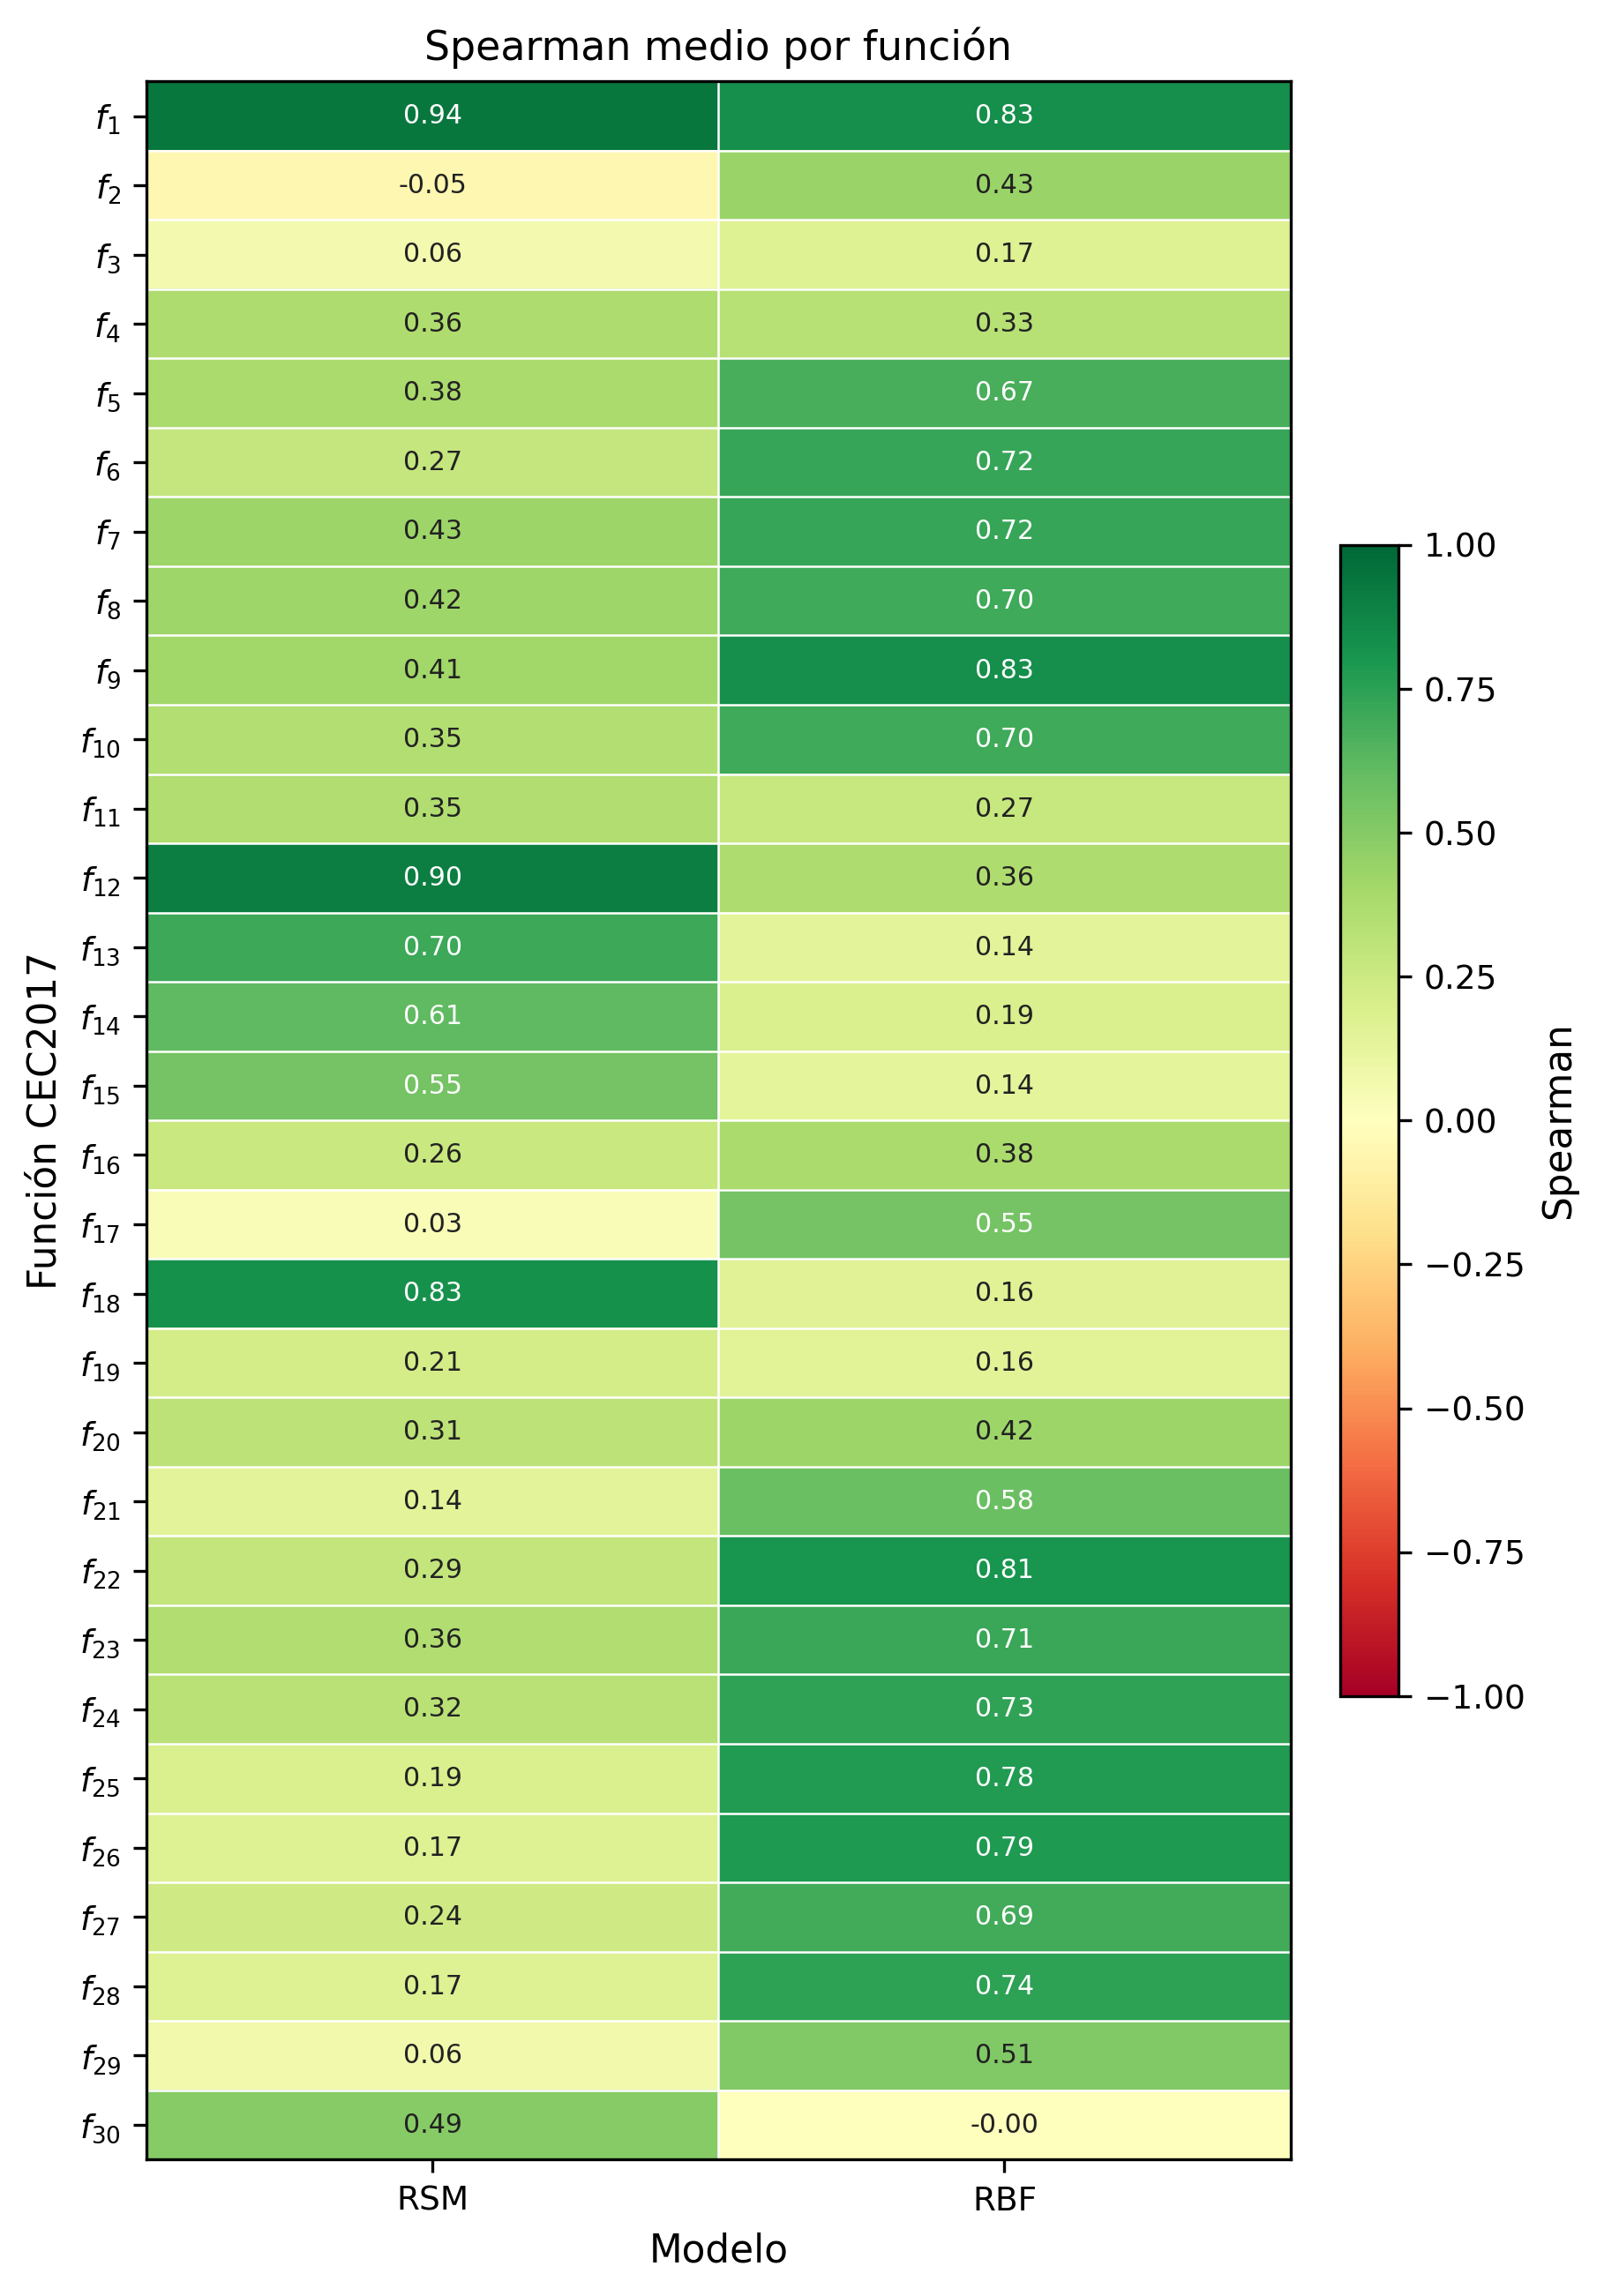
\includegraphics[width=1\textwidth]{figuras/surrogates_offline/heatmap_spearman_final_cec2017.png}
    \caption[Mapa de calor del coeficiente de correlación de Spearman medio por función y modelo]{Mapa de calor del coeficiente de correlación de Spearman medio por función y modelo. El valor anotado en cada celda corresponde al Spearman medio agregado sobre las semillas, los bloques de validación y las metaheurísticas consideradas.}
    \label{fig:heatmap_spearman_final_cec2017}
\end{figure}

A partir de esta figura se observa que ninguno de los dos modelos presenta un comportamiento uniforme en todo el benchmark. Sin embargo, RBF mantiene valores de correlación más estables en un mayor número de funciones, incluidas varias funciones híbridas y compuestas. RSM, por el contrario, concentra su rendimiento en funciones de baja complejidad y muestra una degradación más acusada en problemas de mayor complejidad estructural.

No obstante, los valores medios de nRMSE y nMAE de la
Tabla~\ref{tab:comparativa_configuraciones_ajustadas} resultan elevados en comparación con los observados durante el cribado. Para determinar si este comportamiento es general o está provocado por valores extremos (\textit{outliers}), la Figura~\ref{fig:boxplot_nrmse_final_cec2017} muestra la distribución de los errores en escala logarítmica y la Figura~\ref{fig:heatmap_nrmse_final_cec2017} localiza las funciones que concentran los valores más extremos (\textit{outliers}).

\begin{figure}[htbp]
    \centering
    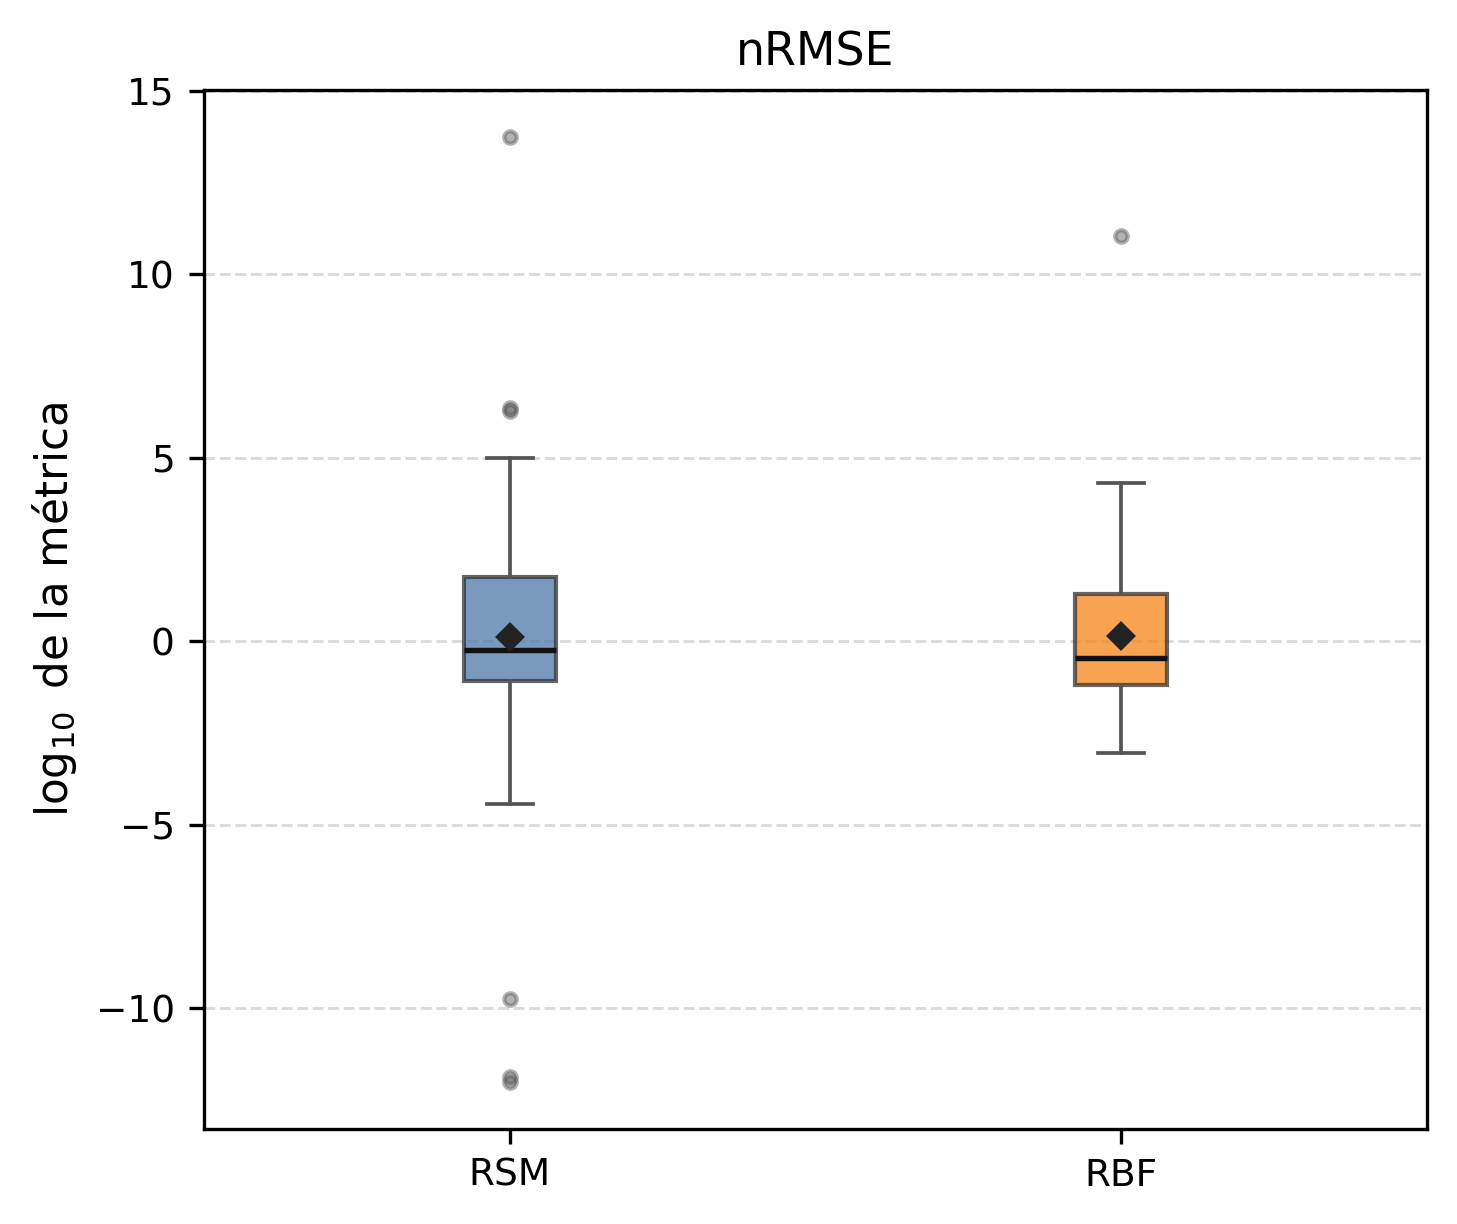
\includegraphics[width=0.9\textwidth]{figuras/surrogates_offline/boxplot_nrmse_final_cec2017.png}
    \caption{Distribución de nRMSE en escala logarítmica para las configuraciones finales de RSM y RBF sobre CEC2017 completa.}
    \label{fig:boxplot_nrmse_final_cec2017}
\end{figure}

\begin{figure}[htbp]
    \centering
    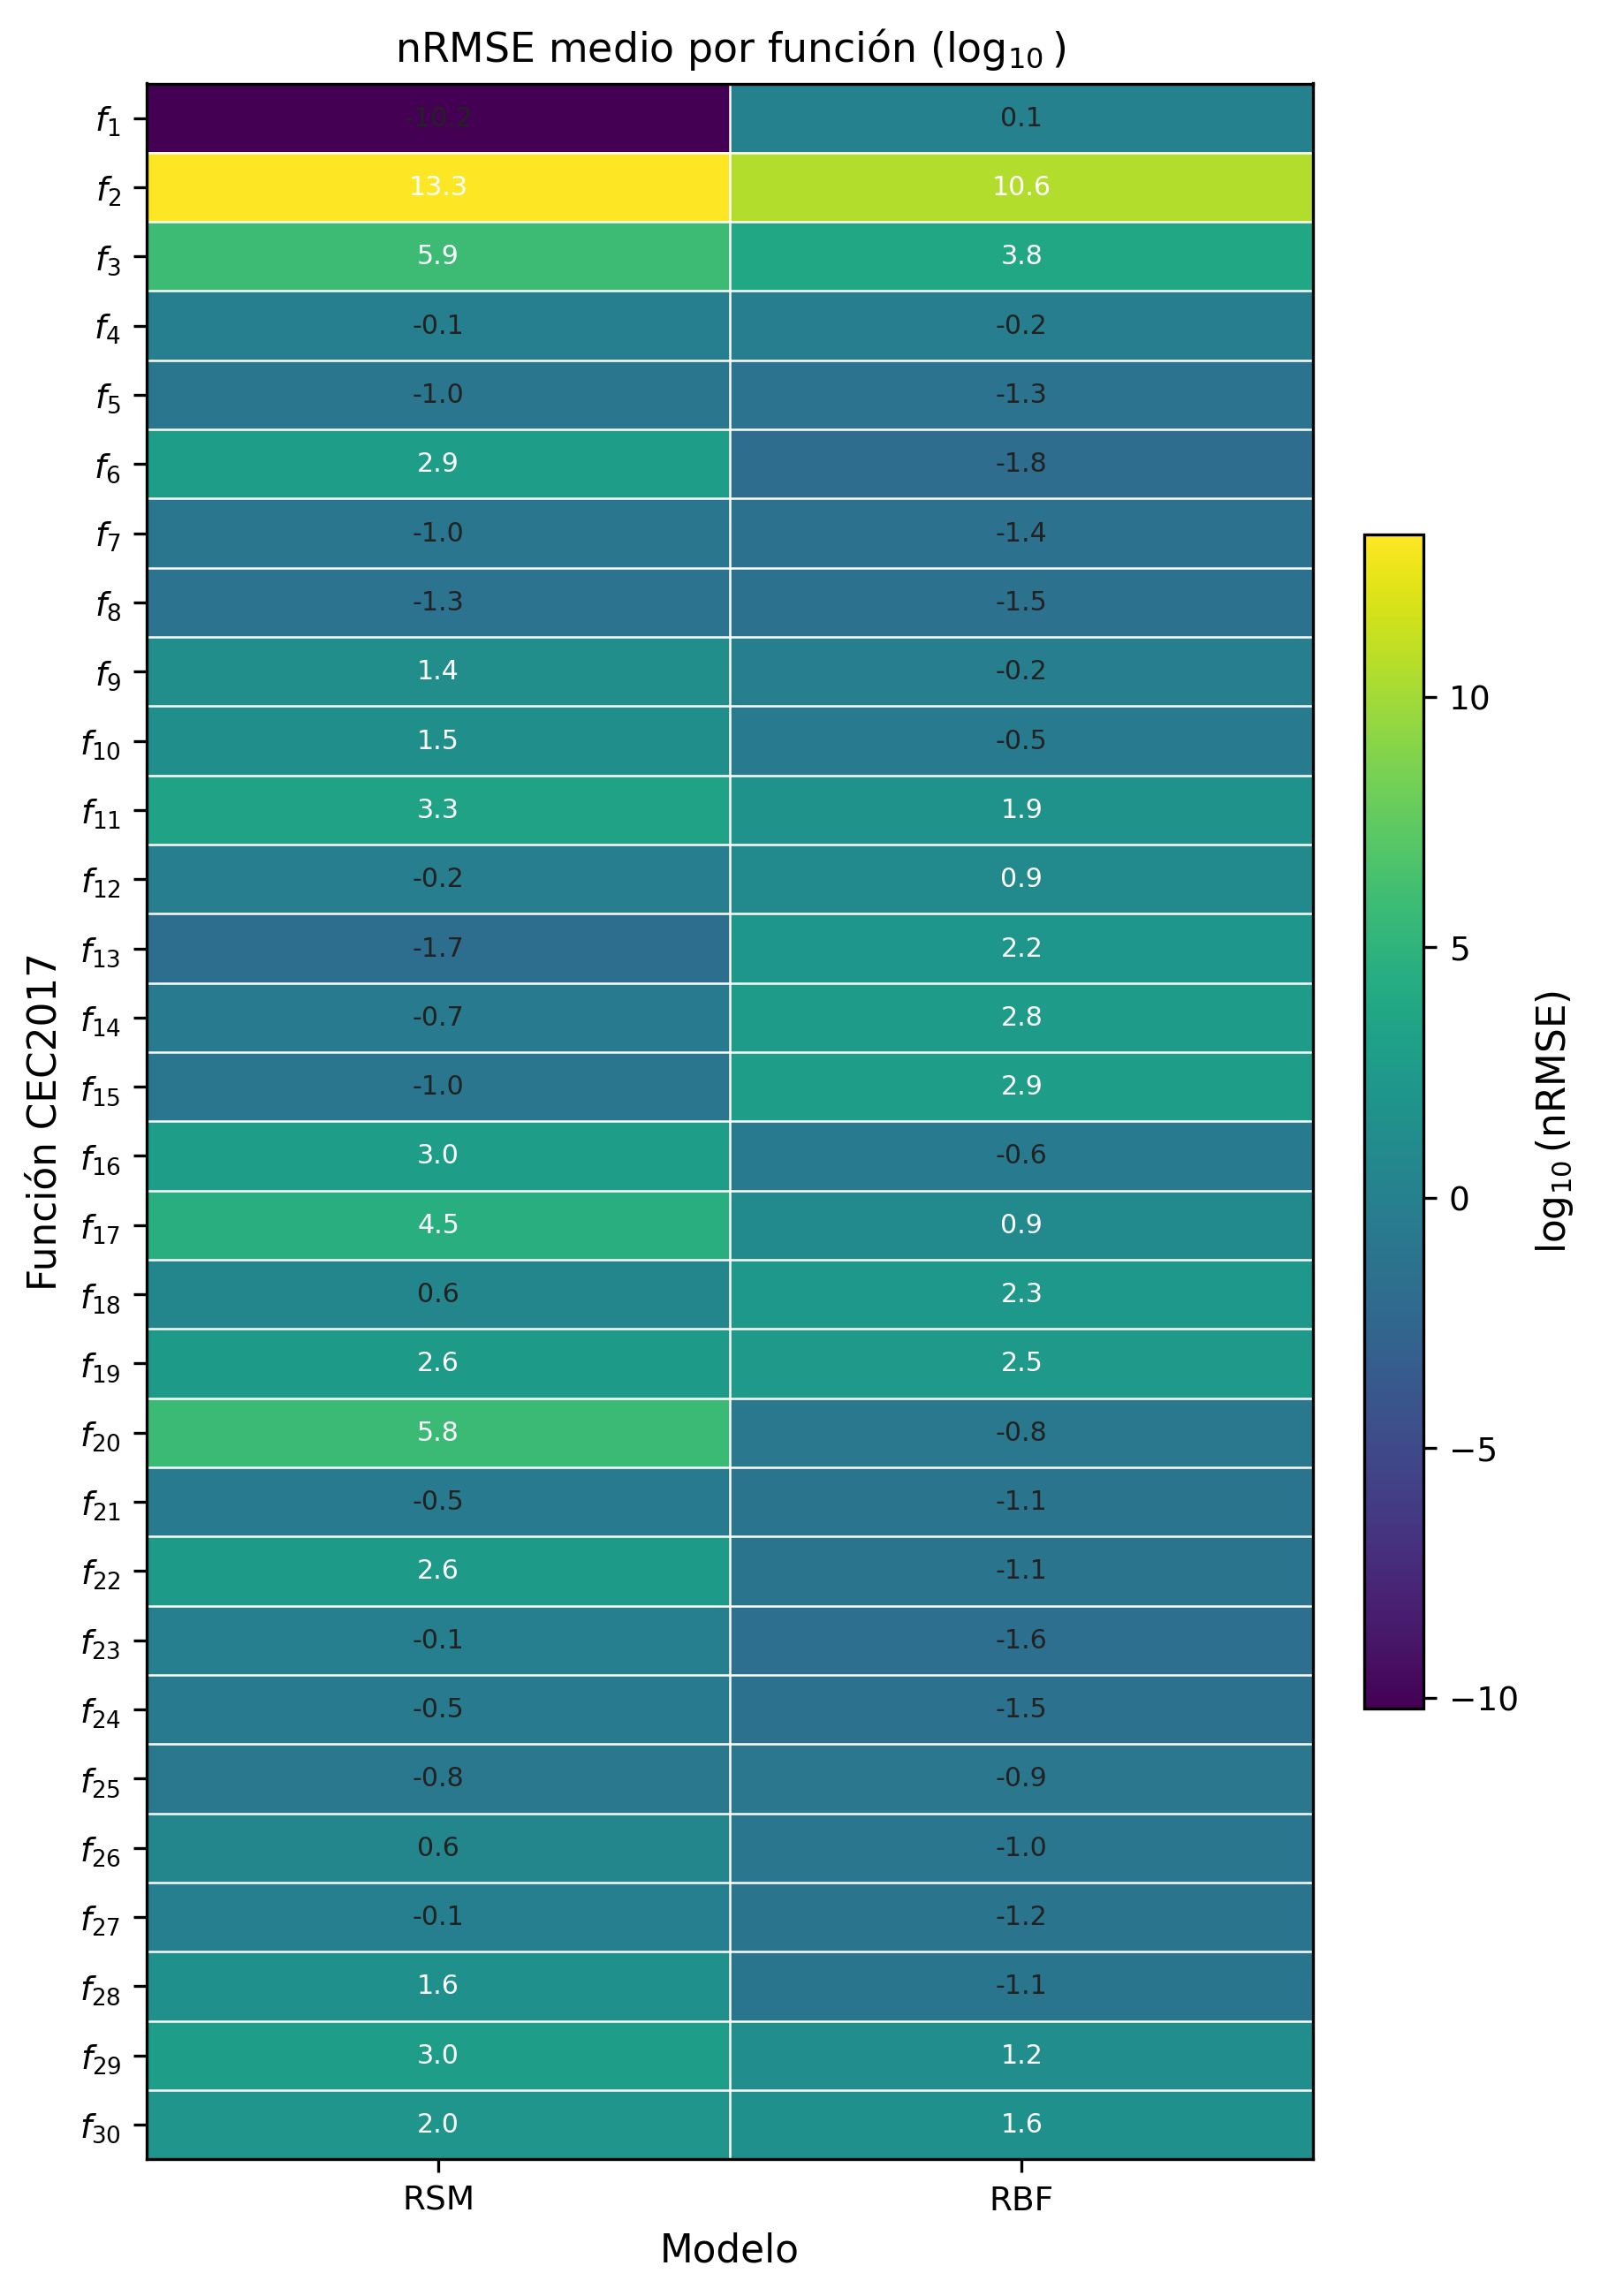
\includegraphics[width=1\textwidth]{figuras/surrogates_offline/heatmap_nrmse_final_cec2017.png}
    \caption{Mapa de calor del nRMSE medio por función y modelo en escala logarítmica.}
    \label{fig:heatmap_nrmse_final_cec2017}
\end{figure}

El \textit{boxplot} demuestra que la media está dominada por \textit{outliers}. La distribución para ambos modelos presenta colas pronunciadas mientras que la mediana se sitúa en rangos más moderados.

Por otro lado, el \textit{heatmap} identifica \(f_2\) como la principal responsable, cuyos valores de nRMSE superan en varios órdenes de magnitud al resto del benchmark en ambos modelos, especialemente para RSM, lo que justifica medias de error superiores. Este comportamiento es coherente con lo indicado en la Sección~\ref{subsec:suite_cec2017}, donde \(f_2\) fue excluida en revisiones posteriores de CEC2017 debido a sus inestabilidades numéricas. En este trabajo se mantiene para respetar la definición experimental del Capítulo~\ref{chap:metodologia_experimental}.

Teniendo en cuenta el análisis realizado, RBF muestra el comportamiento más
adecuado para continuar con la integración \textit{online}. Aunque sus errores
medios se ven afectados por valores extremos, especialmente en \(f_2\), el
modelo mantiene una mayor capacidad de ordenación que RSM sobre la suite
completa. Esta diferencia es especialmente relevante en el contexto de este
trabajo, ya que el objetivo del subrogado no es sustituir de forma exacta a la
función objetivo, sino apoyar la búsqueda preservando el orden relativo entre
soluciones candidatas. Además, su tiempo de entrenamiento es reducido, por lo
que el coste de reajustar el modelo durante la búsqueda no resulta
especialmente limitante. Su principal desventaja se encuentra en el tiempo de
predicción, superior al de RSM, aunque este incremento se considera asumible frente a la
mejora obtenida en la capacidad ordinal.

Este análisis permite extraer una conclusión más general sobre las técnicas
evaluadas, siempre dentro del escenario experimental considerado. Para las
trayectorias generadas sobre CEC2017 con dimensión \(D=10\) y tamaño de
población \(50\), una mayor complejidad del modelo no se traduce
necesariamente en una mejor utilidad como subrogado. En particular, los modelos
clásicos como RBF o RSM parecen adaptarse mejor al criterio principal de
evaluación con un coste computacional controlado, mientras que los modelos de
aprendizaje automático considerados, como los modelos basados en árboles o
redes neuronales, no alcanzan una mejora suficiente en Spearman como para
compensar su complejidad o su coste.

Por tanto, se selecciona \textbf{RBF} como el modelo subrogado para la
fase \textit{online}. RSM queda descartado como alternativa final pese a su bajo
tiempo de predicción, ya que su capacidad de ordenación es menor y su
comportamiento resulta menos estable al ampliar la evaluación al benchmark
completo.

\subsection{Validación del escenario de evaluación}

Tras seleccionar la mejor técnica subrogada sobre trayectorias con reinicio, se comprueba si la elección de un escenario sin reinicio conduciría a conclusiones diferentes o si, por el contrario, dichas trayectorias producen una evaluación menos informativa.

La Tabla~\ref{tab:comparativa_reinicio_surrogate} contrasta los resultados de RBF cuando las metaheurísticas operan con y sin reinicio.

\begin{table}[H]
    \centering
    \small
    \begin{adjustbox}{max width=\textwidth}
        \begin{tabular}{lccccc}
            \toprule
            \textbf{Escenario} & \textbf{Spearman} & \textbf{nRMSE}                  & \textbf{nMAE}                   & \textbf{Entren. (s)} & \textbf{Pred. (s)} \\
            \midrule
            Con reinicio       & \textbf{0.5074}   & \(\mathbf{1.2389 \times 10^9}\) & \(\mathbf{9.5968 \times 10^8}\) & 0.0057               & 0.7076             \\
            Sin reinicio       & 0.5023            & \(7.0201 \times 10^{10}\)       & \(5.1973 \times 10^{10}\)       & \textbf{0.0047}      & \textbf{0.3944}    \\
            \bottomrule
        \end{tabular}
    \end{adjustbox}
    \caption[Comparación de métricas de RBF con y sin reinicio de las metaheurísticas]{Comparación de métricas de RBF con y sin reinicio de las metaheurísticas. Medias calculadas sobre todas las funciones, semillas y bloques de validación.}
    \label{tab:comparativa_reinicio_surrogate}
\end{table}

Los resultados agregados muestran que el escenario con reinicio consigue una capacidad de ordenación ligeramente superior y reduce notablemente los errores medios normalizados respecto a las trayectorias sin reinicio. Aunque este último presenta menores tiempos de entrenamiento y predicción, esta reducción de coste no implica necesariamente una evaluación más adecuada del subrogado para la integración \textit{online}.

Como se demostró en la Sección \ref{sec:resultados_reinicio}, las trayectorias pueden quedar dominadas por fases prolongadas de estancamiento, en las que las muestras de validación presentan valores de \textit{fitness} muy similares entre sí. En esas condiciones, los errores normalizados pueden disminuir artificialmente sin que ello implique que el modelo haya aprendido una aproximación más útil para guiar la búsqueda.

Este efecto se aprecia con claridad en \(f_4\). La Tabla~\ref{tab:ejemplo_f4_sin_reinicio} muestra la evolución del
nMAE medio por bloque temporal para RBF sobre \(f_4\), comparando ambos
escenarios.

\begin{table}[H]
    \centering
    \small
    \begin{tabular}{lcc}
        \toprule
        \textbf{Bloque de entrenamiento} & \textbf{Con reinicio} & \textbf{Sin reinicio} \\
        \midrule
        1--20\%                          & 0.1295                & 0.1267                \\
        21--40\%                         & 0.1140                & 0.0012                \\
        41--60\%                         & 0.0414                & 0.0006                \\
        61--80\%                         & 0.0363                & 0.0004                \\
        \bottomrule
    \end{tabular}
    \caption{nMAE medio de RBF sobre \(f_4\) con y sin reinicio por bloque temporal.}
    \label{tab:ejemplo_f4_sin_reinicio}
\end{table}

En el primer bloque temporal, ambos escenarios presentan errores muy similares. Sin embargo, a partir del segundo bloque el error sin reinicio cae hasta valores prácticamente nulos, mientras que el escenario con reinicio mantiene errores mayores al conservar una trayectoria más variable.

No obstante, este comportamiento no indica que el subrogado haya aprendido una aproximación más útil de la función objetivo, sino que la trayectoria ha alcanzado una región de estancamiento total. En este contexto, las muestras del bloque futuro presentan valores de \textit{fitness} muy próximos, por lo que la tarea de predicción pierde el sentido.

Por tanto, las trayectorias con reinicio constituyen un escenario de evaluación
más exigente y más representativo para el objetivo de este trabajo. Al reactivar
la búsqueda, el reinicio mantiene una mayor variabilidad en las muestras
generadas y evita que la evaluación del subrogado quede condicionada por tramos estancados. En consecuencia, la selección de RBF sobre el
escenario con reinicio se considera metodológicamente más fiable para estudiar
su posterior integración \textit{online}.


\section{Evaluación de la estrategia \textit{online}}
\label{sec:online}

La última fase experimental estudia la integración \textit{online} del modelo \textbf{RBF} seleccionado en las secciones anteriores. Siguiendo el protocolo definido en la Sección~\ref{sec:diseno_online}, primero se calibran los parámetros específicos de la hibridación y, posteriormente, se evalúa su efecto sobre las metaheurísticas consideradas en el escenario con reinicio fijado previamente. El objetivo es comprobar si el filtro subrogado aporta una mejora real frente a la misma metaheurística sin intervención subrogada y si el coste añadido por su
uso resulta asumible.

\subsection{Calibración de los parámetros de integración}

%% no repetimos la definicion de los parámetros. 

En coherencia con los resultados obtenidos en la evaluación \textit{offline}, el subrogado se actualiza utilizando la
información más reciente disponible durante la ejecución.

A partir del protocolo descrito en la Sección~\ref{sec:diseno_online}, se evalúan los valores candidatos de cada parámetro sobre el subconjunto de funciones y semillas definido.

% - piloto de cooldown ya que depende del reinicio
% - piloto de retrain_ratio, porque controla actualizacion/coste del modelo
% - piloto de p, porque regula la agresivididad real del filtro y es el mas importante


% Los resultados muestran que cooldown=x, retrain_ratio=x y p=x ofrecen el mejor compromiso entre error final, ranking medio y coste computacional, por lo que se adoptan como configuración final para la evaluación online completa.

\subsection{Resultados frente a la metaheurística sin filtro}

%%%%%%%%%%%%%%%%%%%%%%%%%%%%%%%%%%%%%%%%%%%%%%%%%%%%%%%%%%%%
%%%%%%%%%%%%%%%%%%%%%%%%%%%%%%%%%%%%%%%%%%%%%%%%%%%%%%%%%%%%
%% resultado importante del trabajo

% - configuración online final seleccionada
% - evaluacion final sobre 30 funciones y 51 semillasnuevas
% - comparacion p=0.00 vs p=0.50

%% el analisis debe responder "la intengracion online mejora realmente el prceso de optimización??"" y por ende, "comprobar si la version mh + subrogado mejora a la version original de cada mh".

%% en ningun momento estamos comparando los evolutivos con el estacionario -> NO NOS IMPORTA PARA NADA. solo nos importa que mejore la hibridacion -> si uno mejora, pues este MEJORA MUCHO y este NO MEJORA TANTO pero YA ESTA.

%% a lo mejor NO MEJORA pero lo que si vamos a ver al 100%, como poco, es que en la curva de convergencia la velocidad si incrementa.
% - esta no mejoria puede deberse a que reinicia demasiadas veces pero podemos justificarlo como: "se han aplicado tecnicas de reinicio pero realmente, si no tuvieramos ese reinicio y nos estabilizasemos cuando ya el algoritmo no mejora mas, estariamos parando MUCHO ANTES que DESPUES --> asi podemos venderlo

% esta claro que si la MH SE ESTANCA, no tiene sentido el papel e integración de los subrogados -> o paramos o aplicamos reinicio


% - Evaluación del ahorro de evaluaciones reales.
% - convergencia
% - Discusión de cuándo ayuda y cuándo perjudica.
%%%%%%%%%%%%%%%%%%%%%%%%%%%%%%%%%%%%%%%%%%%%%%%%%%%%%%%%%%%%
%%%%%%%%%%%%%%%%%%%%%%%%%%%%%%%%%%%%%%%%%%%%%%%%%%%%%%%%%%%%
% - tabla principal
% - analisis
% - parrafo de diagnostico: porcentaje de rechazo, numero de entrenamieto, tiempo online, si el filtro esta siendo demsaido agresivo o razonable...

% ejemplo: Además del error final, los contadores de la integración permiten interpretar el efecto del filtro. En las ejecuciones con \(p=0.50\), el subrogado no reduce el presupuesto total de evaluaciones reales, que se mantiene fijo, sino quedescarta candidatos antes de su evaluación y desplaza el presupuesto hacia otros candidatos generados posteriormente. Por tanto, el porcentaje de rechazo y el tiempo dedicado al modelo permiten valorar si la mejora obtenida compensa la intervención del filtro.

% - Si mejora el error final y rechaza muchos candidatos: el filtro está funcionando bien.
% - Si empeora y rechaza muchos candidatos: probablemente está descartando candidatos útiles.
% - Si apenas rechaza candidatos: el subrogado interviene poco y su impacto será limitado.
% - Si el tiempo online sube mucho: aunque mejore algo, puede no compensar.
%%%%%%%%%%%%%%%%%%%%%%%%%%%%%%%%%%%%%%%%%%%%%%%%%%%%%%%%%%%%
%%%%%%%%%%%%%%%%%%%%%%%%%%%%%%%%%%%%%%%%%%%%%%%%%%%%%%%%%%%%



%% criterio de reinicio - cooldown

% por la definicion de criterio de reactivacion que se ha definido y por los resultados obtenidos en este mismo capitulo cuando hablamos de la motivacion del reinciio y analizamos graficas tras aplicarlo posteriromente, se podia ver que la poblacion cambiaba bruscamente, por ese motivo, se considera evaluar..

% Si el subrogado se usa inmediatamente, puede estar entrenado sobre una distribución que ya no representa la nueva población.

% Por ello se introduce un periodo de enfriamiento o cooldown, durante el cual se priorizan evaluaciones reales antes de volver a confiar en el modelo.

% La inclusión de un periodo de enfriamiento tras el reinicio se justifica tanto
% por la definición del propio mecanismo como por el comportamiento observado en
% los experimentos anteriores. El reinicio elitista conserva únicamente la mejor
% solución encontrada y regenera el resto de la población, por lo que introduce un
% cambio abrupto en la distribución de candidatos disponibles. Este efecto ya se
% aprecia en el análisis del reinicio realizado al comienzo de este capítulo,
% donde la reactivación de la población modifica la dinámica de convergencia y de
% diversidad. En consecuencia, utilizar inmediatamente un subrogado entrenado con
% muestras anteriores al reinicio podría conducir a predicciones poco
% representativas. Por este motivo, se incorpora como parámetro experimental un
% periodo de enfriamiento durante el cual se retrasa el uso del subrogado y se
% prioriza la generación de nuevas evaluaciones reales.

% La conclusión clara es que la hibridación con p=0.50 no mejora de forma homogénea a las tres metaheurísticas. Funciona mejor en DE, no compensa en AGE y queda muy cerca de neutra en SHADE.

% Para AGE, el filtro rechaza bastantes candidatos, alrededor del 64.7%, pero el rendimiento final empeora. Eso apunta a que el subrogado está interviniendo de forma efectiva, pero no de forma beneficiosa: probablemente descarta candidatos que sí podían ser útiles para la dinámica estacionaria de AGE.

% Para DE, el resultado es el más favorable. p=0.50 gana muchas más veces de las que pierde y mejora el ranking medio. Aun así, hay que matizar que la media empeora por funciones con outliers, especialmente en funciones compuestas como f30. Por eso, para DE la lectura correcta es: mejora robusta en términos pareados/ranking/mediana, pero con coste computacional alto y sensibilidad en algunos casos.

% Para SHADE, no hay una mejora suficientemente clara. El ranking medio queda casi empatado y las pérdidas superan ligeramente a las mejoras. Aquí el filtro interviene mucho, con rechazo cercano al 74%, pero no se traduce en una mejora final estable.

% De cara a la memoria, yo lo redactaría así: la configuración p=0.50 seleccionada en pilotos muestra que la integración online puede aportar valor, pero su efecto depende de la metaheurística. La evidencia más favorable aparece en DE; en AGE resulta perjudicial y en SHADE no ofrece una ventaja clara. Esto es una conclusión fuerte y honesta para la sección final online.


% El piloto de enfriamiento tras reinicio muestra que introducir una pausa después del reinicio resulta beneficioso frente a activar el filtro inmediatamente. Entre los valores evaluados, \(100\) evaluaciones ofrece el mejor compromiso agregado: obtiene el mejor ranking medio en AGE, DE y SHADE y concentra el mayor número de funciones ganadas. Valores menores parecen insuficientes para estabilizar la nueva región explorada, mientras que valores mayores retrasan en exceso la intervención del subrogado


% La calibración se realiza de forma secuencial, no como una búsqueda exhaustiva sobre todas las combinaciones posibles. Por tanto, los valores seleccionados no deben interpretarse como óptimos globales, sino como una configuración homogénea y computacionalmente viable para evaluar la integración online en las tres metaheurísticas.

% El valor de enfriamiento se estudia manteniendo fijos el resto de parámetros de integración. Bajo esta configuración de referencia, \(100\) evaluaciones proporciona el mejor comportamiento agregado, por lo que se adopta como valor base para los pilotos posteriores.

\subsection{Comparación con técnicas subrogadas de referencia}

% - comparacion con técnicas de referencia como kriging y pce

%%%%%%%%%%%%%%%%%%%%%%%%%%%%%%%%%%%%%%%%%%%%%%%%%%%%%%%%%%%%
%%%%%%%%%%%%%%%%%%%%%%%%%%%%%%%%%%%%%%%%%%%%%%%%%%%%%%%%%%%%
%% comparación breve

%% rbf online, kriging online, pce online y p=0 como referencia.
%% no haremos una discusion larga modelo a modelo. el objetivo es comprobar si RBF, elegido mediante la fase offline y ya demostrado su mejor rendimiento frente a modelos de aprendizaje automatico mas complejos tratados como subrogados, tambn es competitivo frente a técnicas clasicas en integracion real --> tenemos un algoritmo que es mas complejo y no es necesario ya que tenemos una tecnica matematica que va mejor, por ejemplo.
%%%%%%%%%%%%%%%%%%%%%%%%%%%%%%%%%%%%%%%%%%%%%%%%%%%%%%%%%%%%
%%%%%%%%%%%%%%%%%%%%%%%%%%%%%%%%%%%%%%%%%%%%%%%%%%%%%%%%%%%%
\subsection{Conclusiones de la integración \textit{online}}


%% cerrar brevemente con varias ideas:

%% si la hibridacion mejora o no mejora frente a la metaheuristica base
%% si el coste añadido es razonable
%% si el filtro es lo suficientemente robusto para las metaheuristicas consideradas o si su utilidad depende del algoritmo.










% Por qué el Spearman alto sin reinicio es engañoso:

% Cuando la metaheurística se estanca, la población converge a una región pequeña del espacio. Los valores de fitness de soluciones vecinas son muy similares y localmente suaves. Predecir el orden relativo de
% puntos casi idénticos es un problema trivial para cualquier modelo — el Spearman sube porque la tarea es más fácil, no porque el subrogado sea más útil.

% La evidencia más clara la tienes en las medianas de nRMSE: 0.0004 sin reinicio frente a 0.8389 con reinicio en las mismas funciones. Esa diferencia de tres órdenes de magnitud en el error típico es
% precisamente la huella de ese efecto: sin reinicio, los valores de fitness son tan parecidos entre sí que los errores absolutos son mínimos.


% El punto clave para tu TFG:

% El escenario relevante para la integración online es el de trayectorias dinámicas — con reinicios, cambios de región y alta diversidad de muestras. Evaluar el subrogado sobre trayectorias estancadas produce
% una estimación optimista que no se corresponde con el contexto real de uso. Por tanto, comparar ambos escenarios para elegir el modelo sería metodológicamente incorrecto.

% Una matiz que conviene tener presente:

% La diferencia en Spearman entre escenarios no es dramática (0.80 vs 0.74 en mediana), lo que refuerza el argumento: el subrogado no "pierde" capacidad porque hay reinicio, sino que se enfrenta a un problema
% más exigente y realista. Eso es lo que hay que transmitir en el texto si decides incluir esta comparación.
%% conclusion:
% - resumen de contribuciones
% - conclusiones principales
% - trabajo futuro

\chapter{Conclusiones y trabajo futuro}
\label{chap:conclusion}

% TODO: sección de conclusiones (pendiente de resultados experimentales)

\section{Trabajo futuro}
\label{sec:trabajo_futuro}

A partir del trabajo desarrollado en este Trabajo de Fin de Grado, se identifican varias líneas de extensión
que podrían abordarse en investigaciones posteriores.

\begin{itemize}

    \item \textbf{Extensión a problemas de optimización multiobjetivo.} En los últimos
          años se observa un crecimiento notable en la literatura relacionada con la aplicación
          de técnicas subrogadas a problemas con múltiples objetivos en conflicto. El
          enfoque desarrollado en este trabajo se ha centrado en optimización de objetivo único,
          lo que deja abierta una posible extensión hacia el ámbito multiobjetivo.

    \item \textbf{Criterios de activación adaptativos para la hibridación \textit{online}.}
          En la hibridación \textit{online} propuesta, la decisión de evaluar una solución
          candidata con el subrogado o con la función real se rige mediante una
          probabilidad fija. Una posible mejora consistiría en sustituir este mecanismo por
          un criterio adaptativo que tome en consideración el estado actual de la búsqueda o
          la fiabilidad estimada del modelo, recurriendo a la evaluación real únicamente cuando
          la predicción del subrogado no ofrezca suficientes garantías. Este tipo de
          enfoque permitiría reducir aún más el número de evaluaciones reales sin comprometer
          la calidad de las soluciones obtenidas.

    \item \textbf{Análisis de la estabilidad temporal de los modelos subrogados.}
          La evaluación \textit{offline} desarrollada permite estudiar la capacidad de los
          modelos para anticipar la etapa inmediatamente posterior de la búsqueda. Como
          ampliación, resultaría de interés evaluar por separado su rendimiento sobre
          horizontes temporales progresivamente más alejados del conjunto de entrenamiento.
          Este análisis permitiría estimar durante cuánto tiempo siguen siendo útiles las
          relaciones aprendidas por el subrogado y determinar con mayor precisión la
          frecuencia de reentrenamiento más adecuada para su integración \textit{online},
          especialmente ante los cambios introducidos por los mecanismos de reinicio.

    \item \textbf{Muestreo inicial mediante \textit{Latin Hypercube Sampling}.} La
          estrategia \textit{online} desarrollada construye el conjunto de entrenamiento del
          subrogado a partir de las soluciones generadas por la propia metaheurística
          durante su ejecución, lo que implica un periodo inicial en el que el modelo no está
          disponible. Una alternativa que permitiría integrarlo desde la primera evaluación
          consistiría en generar un conjunto inicial de puntos mediante \textit{Latin Hypercube
              Sampling} (LHS), una técnica de muestreo que distribuye los puntos de forma más
          representativa que el muestreo aleatorio puro. Estos puntos se evaluarían con la
          función real antes de iniciar la metaheurística, proporcionando al subrogado
          una visión más amplia del espacio de búsqueda desde el comienzo.

\end{itemize}


% bibliografía
% ------------------

\bibliography{bibliografia/bibliografia}
\addcontentsline{toc}{chapter}{Bibliografía}
\bibliographystyle{unsrturl}

% apendice
% ------------------
\appendix
% \input{apendices/A_detalles_experimentales}
% \input{apendices/B_tablas_completas}
% apendice
% ------------------

\input{apendices/B_tablas_tacolab_reinicio}

% \input{apendices/C_boxplots_seed}
% \input{apendices/D_manual_reproduccion}

% \input{capitulos/04_diseno_metodologico}
% \input{capitulos/05_implementacion}
% \input{capitulos/06_analisis_metaheuristicas}
% \input{capitulos/07_resultados_no_acumulativo}
% \input{capitulos/08_resultados_acumulativo}
% \input{capitulos/09_discusion}
% \input{capitulos/10_conclusiones}

%\input{capitulos/01_Introduccion}
%
%\input{capitulos/02_EspecificacionRequisitos}
%
%\input{capitulos/03_Planificacion}
%
%\input{capitulos/04_Analisis}
%
%\input{capitulos/05_Diseno}
%
%\input{capitulos/06_Implementacion}
%
%\input{capitulos/07_Pruebas}
%
%\input{capitulos/08_Conclusiones}
%
%%\chapter{Conclusiones y Trabajos Futuros}
%
%
%%\nocite{*}
% \bibliography{bibliografia/bibliografia}\addcontentsline{toc}{chapter}{Bibliografía}
% \bibliographystyle{miunsrturl}
%
%\appendix
%\input{apendices/manual_usuario/manual_usuario}
%%\input{apendices/paper/paper}
%\input{glosario/entradas_glosario}
% \addcontentsline{toc}{chapter}{Glosario}
% \printglossary
\chapter*{}
\thispagestyle{empty}

\end{document}
